%%% Presentation slides
\newcommand{\slidesfinal}{
  \documentclass[handout,style=authortitle]{beamer}
}

%%% Ignore images --- slightly faster compilation
\newcommand{\slidestest}{
  \documentclass[demo,handout,style=authortitle]{beamer}
}

%%% Printable slides with side notes thing
\newcommand{\makehandouts}{
  \usepackage{handoutWithNotes}
  \usepackage{pgfpages}
  \pgfpagesuselayout{3 on 1 with notes big}[a4paper,border shrink=7mm]
  \pgfpageslogicalpageoptions{1}{border code=\pgfusepath{stroke}}
  \pgfpageslogicalpageoptions{2}{border code=\pgfusepath{stroke}}
  \pgfpageslogicalpageoptions{3}{border code=\pgfusepath{stroke}}
}
\slidesfinal
% \slidestest
% \makehandouts

%%% Styles and settings
% -------------------------------------------------------------------------
% Author, title, etc.
% -------------------------------------------------------------------------

% author
\makeatletter
\newcommand\myshortauthor[1]{\renewcommand\@myshortauthor{#1}}
\newcommand\@myshortauthor{}
\makeatother

\makeatletter
\newcommand\myauthor[1]{\renewcommand\@myauthor{#1}}
\newcommand\@myauthor{}
\makeatother

\makeatletter
\author[\theauthorgoeshere]{\@myauthor}
\makeatother

% url
\makeatletter
\newcommand\myurl[1]{\renewcommand\@myurl{#1}}
\newcommand\@myurl{}
\makeatother

% title
\makeatletter
\newcommand\myfulltitle[1]{\renewcommand\@myfulltitle{#1}}
\newcommand\@myfulltitle{}
\makeatother

\makeatletter
\newcommand\myabbrvtitle[1]{\renewcommand\@myabbrvtitle{#1}}
\newcommand\@myabbrvtitle{}
\makeatother

% \makeatletter
% \newcommand\mytitle[1]{\renewcommand\@mytitle{#1}}
% \newcommand\@mytitle{}
% \makeatother

% date
\makeatletter
\newcommand\mydate[1]{\renewcommand\@mydate{#1}}
\newcommand\@mydate{}
\makeatother


% maketitle
\makeatletter
\newcommand{\mytitlea}{\makebox[.45\paperwidth]%
{\@myabbrvtitle\hfill\insertframenumber/\inserttotalframenumber}}
\newcommand{\mytitleb}{\@myabbrvtitle}
\makeatother


\makeatletter
\title[\mytitleb]{\@myfulltitle}
\makeatother


\makeatletter
\date{\@mydate \\[.5cm] \titlelogos}
\makeatother

\makeatletter
\newcommand{\theauthorgoeshere}{\makebox[.45\paperwidth]{%
        \@myurl \hfill \@myshortauthor}}
\makeatother

%\documentclass{beamer}
\documentclass[handout]{beamer}

\usepackage{amsmath}
\usepackage{beamerthemesplit}
\usepackage{fancybox}
\usepackage{hyperref}
\usepackage{color}
\usepackage{listings}


\makeatletter
\newcommand\code{\bgroup\@makeother\_\@makeother\~\@makeother\$\@codex}
\def\@codex#1{{\normalfont\ttfamily\hyphenchar\font=-1 #1}\egroup}
\makeatother

\newcommand{\bX}{\boldsymbol{X}}
\newcommand{\bx}{\boldsymbol{x}}
\newcommand{\by}{\boldsymbol{y}}
\newcommand{\bbeta}{\boldsymbol{\beta}}
\newcommand{\bepsilon}{\boldsymbol{\epsilon}}
\newcommand{\bs}[1]{\boldsymbol{#1}}


\definecolor{gray}{rgb}{.6,.6,.6}
\definecolor{orange}{rgb}{1,0.5,0}
\definecolor{grayish}{rgb}{.775, .775, .775}
\definecolor{dkgray}{rgb}{.375, .375, .375}
\definecolor{dkgreen}{rgb}{0,0.6,0}
\definecolor{mauve}{rgb}{0.58,0,0.82}
\definecolor{dkblue}{rgb}{0, 0, .5}
\definecolor{purple}{rgb}{0.7, 0, 0.5}

\definecolor{g11}{rgb}{0, 0, 1}
\definecolor{g12}{rgb}{0, .4, 1}
\definecolor{g13}{rgb}{0, .8, 1}

\definecolor{g21}{rgb}{0, .5, .3}
\definecolor{g22}{rgb}{.4, .5, .3}
\definecolor{g23}{rgb}{.8, .5, .3}

\lstset{ %
  language=R,     
  numbers=left,
  stepnumber=1,       
  numbersep=6pt,      
  showspaces=false,      
  showstringspaces=false,  
  showtabs=false,    
  frame=single,      
  rulecolor=\color{black},   
  tabsize=4,     
  captionpos=t,     
  breaklines=true,     
  breakatwhitespace=true,   
  title=\lstname,              
  basicstyle=\ttfamily\color{black}\scriptsize, 
  backgroundcolor=\color{grayish},  
  numberstyle=\tiny\color{black},  
  keywordstyle=\color{blue}, 
  commentstyle=\color{dkgreen}, 
  stringstyle=\color{mauve}, 
  xleftmargin=.1in,
  xrightmargin=.1in,
  aboveskip=0cm,
  belowskip=.2cm
  %   escapeinside={\%*}{*)},    
%   morekeywords={*,...}    
}

\setbeamertemplate{navigation symbols}{} 

\hypersetup{
    linkcolor=,
    colorlinks=true,
    urlcolor=blue
}

\usetheme{Frankfurt}
% \usecolortheme{whale}
% \usetheme{Antibes}
% \setbeamertemplate{mini frames}{}


\newcommand{\fctn}[1]{\textcolor{green!50!blue}{#1}}
\newcommand{\rfor}[1]{\textcolor{yellow!50!red}{#1}}
\newcommand{\rcom}[1]{\textcolor{blue}{#1}}

\newcommand{\pkg}[1]{\textbf{#1}}

\newcommand{\startr}{\begin{minipage}{.04\textwidth}\ \ \end{minipage} \begin{minipage}{.91\textwidth}}

%
\newcommand{\shownum}{\title[\mytitlea]}{}
\newcommand{\hidenum}{\title[\mytitleb]{}}
% \expandafter\def\expandafter\insertshorttitle\expandafter{\insertshorttitle\hfill\insertframenumber\,/\,\inserttotalframenumber}
 

\newcounter{excount}
\setcounter{excount}{0}
\newcommand{\countex}{\addtocounter{excount}{1}\arabic{excount}}
\newcommand{\showex}{\arabic{excount}}






\useoutertheme{miniframes}
\makeatletter
  \beamer@compressfalse
\makeatother

\title{From 1 core to Thousands: R to pbdR}
\author[http://r-pbd.org \hspace{2.5cm}  pbdR Core]{%
  George Ostrouchov$^{1,2}$ and Drew Schmidt$^2$
%  and Wei-Chen Chen$^1$,
%  and Pragneshkumar Patel$^2$
\\[1em]
{$^1$Oak Ridge National Laboratory, Oak Ridge, TN} \\
{$^2$University of Tennessee, Knoxville, TN} \\[5em]
OLCF Workshop \\ on  Processing and Analysis of Very Large Data Sets \\
August 8, 2013}
\date{}
\logo{
  \begin{tabular}{r}
    
\includegraphics[height=.34cm]{../common/pics/ornl.jpg} \\
    
\includegraphics[height=.34cm]{../common/pics/utk_logo.png}
  \end{tabular}
}

\newcommand{\mytitlea}{Programming with Big Data in R \hspace{5em} \insertframenumber\,/\,\inserttotalframenumber}
\newcommand{\mytitleb}{Programming with Big Data in R}

%%%%%%%%%%%%%%%%%%%%%%%%%%%%%%%%%%%%%%%%%%%%%%%%%%%%%%%%%%%%%%%%%%%%%%%%%%%%%%%%%
%%%%%%%%%%%%%%%%%%%%%%%%%%%%%%%%%%%%%%%%%%%%%%%%%%%%%%%%%%%%%%%%%%%%%%%%%%%%%%%%%
%%%%%%%%%%%%%%%%%%%%%%%%%%%%%%%%%%%%%%%%%%%%%%%%%%%%%%%%%%%%%%%%%%%%%%%%%%%%%%%%%
\begin{document}

%%%%%%%%%%%%%%%%%%%%%%%%%%%%%%%%%%%%%%%%
%%     Title and ToC
%%%%%%%%%%%%%%%%%%%%%%%%%%%%%%%%%%%%%%%%
% titlepage
\frame{\maketitle}

\setcounter{footnote}{0}

\begin{frame}[noframenumbering]
\frametitle{The \pbdR\ Core Team}
\begin{minipage}{1\textwidth}
  \vspace{-.6cm}
\begin{minipage}{3.6cm}
\ \\[.8cm]
Wei-Chen Chen$^1$ \\
George Ostrouchov$^{2,3}$ \\
Pragneshkumar Patel$^3$ \\
Drew Schmidt$^3$\\[2ex]
\end{minipage}
\begin{minipage}{7cm}
  \ \hfill 
\includegraphics[width=5.5cm]{../common/pics/logos/newpbdr}
\end{minipage}
\end{minipage}
  \begin{minipage}{2.2cm}\tiny
    $^1$FDA\\
    Washington, DC, USA
  \end{minipage}
  \hspace{1ex}
  \begin{minipage}{5cm}\tiny
    $^2$Computer Science and Mathematics Division\\
    Oak Ridge National Laboratory, Oak Ridge TN, USA
  \end{minipage}
  \hspace{1ex}
  \begin{minipage}{4cm}\tiny
    $^3$Joint Institute for Computational Sciences\\
    University of Tennessee, Knoxville TN, USA
  \end{minipage}

\begin{block}{Support}\tiny
  This material is based upon work supported by the National Science
  Foundation Division of Mathematical Sciences under Grant No. 1418195.
  This work used resources of the \textcolor{blue}{National Institute for
  Computational Sciences} at the University of Tennessee, Knoxville,
  which is supported by the Office of Cyberinfrastructure of the
  U.S. National Science Foundation under Award  No. ARRA-NSF-OCI-0906324
  for NICS-RDAV center.
  This work also used resources of the \textcolor{blue}{Oak Ridge
  Leadership Computing Facility} at the Oak Ridge National
  Laboratory, which is supported by the Office of Science of the
  U.S. Department of Energy under Contract No. DE-AC05-00OR22725.\\[.2cm]
\end{block}
\end{frame}

\begin{frame}
  \frametitle{About This Presentation}
  \begin{block}{Downloads}\scriptsize
    You can update the \pbdR presentations and scripts in your virtual
    machine with: \\ \tt
    \$ cd \\
    \$ scp USERNAME@anselm.it4i.cz:/home/adios/slides/pbdr\_overview.pdf slides \\
    \$ scp
    USERNAME@anselm.it4i.cz:/home/adios/slides/pbdr\_tutorial.pdf
    slides \\
    rm -r scripts \\
    \$ scp -r USERNAME@anselm.it4i.cz:/home/adios/pbdR/scripts .
 \end{block}
\end{frame}

% \begin{frame}
% \frametitle{About This Presentation}
%   \begin{block}{Tutorial Evaluations}
%     \begin{center}
%       \url{http://bit.ly/sc13-tut-mf08}
%     \end{center}
%   \end{block}
% \end{frame}


\begin{frame}
\frametitle{About This Presentation}
 \begin{block}{Installation Instructions}
  Installation instructions for setting up a \pbdR environment are available:
  \begin{center}
  \url{http://r-pbd.org/install.html}
  \end{center}
  This includes instructions for installing R, MPI, and \pbdR.
 \end{block}
\end{frame}

% \begin{frame}%[allowframebreaks=0.8]
% \frametitle{About This Presentation}
%  \begin{block}{Conventions}
%   \begin{itemize}
%     \item We use ``{\Huge$ .$}'' as a decimal mark, not ``{\Huge$,$}''.  E.g.,
% 	``one thousand and one half'' is written ``$1,000.5$'', not ``$1.000,5$''.
%     \item We will use special suffixes to denote distributed objects (ones not
% 	stored entirely on a single processor).\\
%     \code{.spmd} denotes a distributed object, while\\
%     \code{.dmat} denotes a distributed object which is of class
% 	\code{ddmatrix}\\
%     No suffix means the object is global (common to all processors)\\[.2cm]
%     Neither of these suffices carries semantic meaning.
%     \end{itemize}
%  \end{block}
% \end{frame}



% \begin{frame}[fragile]
% \frametitle{About This Presentation}
%  \begin{block}{Conventions For Code Presentation}
% We will use two different forms of syntax highlighting.  One for displaying
% results from an interactive R session:
% \begin{lstlisting}[backgroundcolor=\color{white},basicstyle=\ttfamily\color{
% dkgray}\scriptsize,keywordstyle=\color{black},
%   commentstyle=\color{orange},stringstyle=\color{mauve}]
% R> "interactive"
% [1] "interactive"
% \end{lstlisting}
% and one for presenting R scripts
% \begin{lstlisting}
% "not interactive"
% \end{lstlisting}
%  \end{block}
% \end{frame}



\begin{frame}[noframenumbering,shrink]
\frametitle{Contents}
\small
\tableofcontents[hideallsubsections]
\end{frame}

\setcounter{framenumber}{0}
\section{Introduction}
\makesubcontentsslides


%%% Hardware slides
% \input{misc/hardware}


%%% Intro to parallelism
% \input{misc/parallelism}



\subsection{R and Parallelism}


\begin{frame}
%  \addtocounter{framenumber}{-1}
  \begin{block}{R and Parallelism}\pause
  What about R?
  \end{block}
\end{frame}

\begin{frame}
%  \addtocounter{framenumber}{-1}
  \begin{block}{Problems with Serial R}\pause
  \begin{enumerate}[<+-|alert@+>]
    \item Slow.
    \item If you don't know what you're doing, it's \emph{really} slow.
    \item Performance improvements usually for small machines.
    \item Very ram intensive.
  \end{enumerate}
  \end{block}
\end{frame}


\begin{frame}
  \begin{block}{Why We Need Parallelism}\pause
    \begin{enumerate}[<+-|alert@+>]
      \item Saves compute time.
      \item Data size is skyrocketing.
      \item Necessary for many problems.
      \item Its necessity is coming.
      \item \emph{It's really cool.}
  \end{enumerate}
  \end{block}
\end{frame}

\begin{frame}
  \begin{block}{Recall: Parallel R Packages}
   \begin{center}
    \begin{minipage}{.45\textwidth}
    \begin{block}{Shared Memory}
      \begin{enumerate}[<+-|alert@+>]
        \item \pkg{foreach}
        \item \pkg{parallel}
        \item \pkg{snow}
        \item \pkg{multicore}
      \end{enumerate}
    \end{block}
    \end{minipage}
    \hspace{.2cm}
    \begin{minipage}{.45\textwidth}
    \begin{block}{Distributed}
      \begin{enumerate}[<+-|alert@+>]
        \item \pkg{Rmpi}
        \item R+Hadoop
        \item \pkg{pbdR}
      \end{enumerate}
    \end{block}
    \end{minipage}
    \end{center}
    (and others\dots)
    \end{block}
\end{frame}



\begin{frame}[shrink]
  \begin{block}{R and Parallelism}
    The solution to many of R's problems is parallelism.  However \dots\vspace{-.4cm}
   \begin{center}
    \begin{minipage}[t]{.95\textwidth}
    \begin{block}{\centering What we have}
      \begin{enumerate}[<+-|alert@+>]
        \item Mostly serial.
        \item Mostly not distributed
        \item Data parallelism mostly explicit
      \end{enumerate}
    \end{block}
    \end{minipage}
    \\\pause
    \begin{minipage}[t]{.95\textwidth}
    \begin{block}{\centering What we want}
      \begin{enumerate}[<+-|alert@+>]
        \item Mostly parallel.
        \item Mostly distributed.
        \item Mostly implicit.
      \end{enumerate}
    \end{block}
    \end{minipage}
    \end{center}
    \end{block}
\end{frame}



\begin{frame}
  \begin{block}{R and Parallelism}
    Likewise, the HPC community is looking for high-level languages for data\dots
    \end{block}
\end{frame}


\section{pbdR}
\makesubcontentsslides

\subsection{The pbdR Project}
\makesubcontentsslidessec

\begin{frame}{\pbdR Interfaces to Libraries: Sustainable Path}
  \vspace{-1ex}
  \centering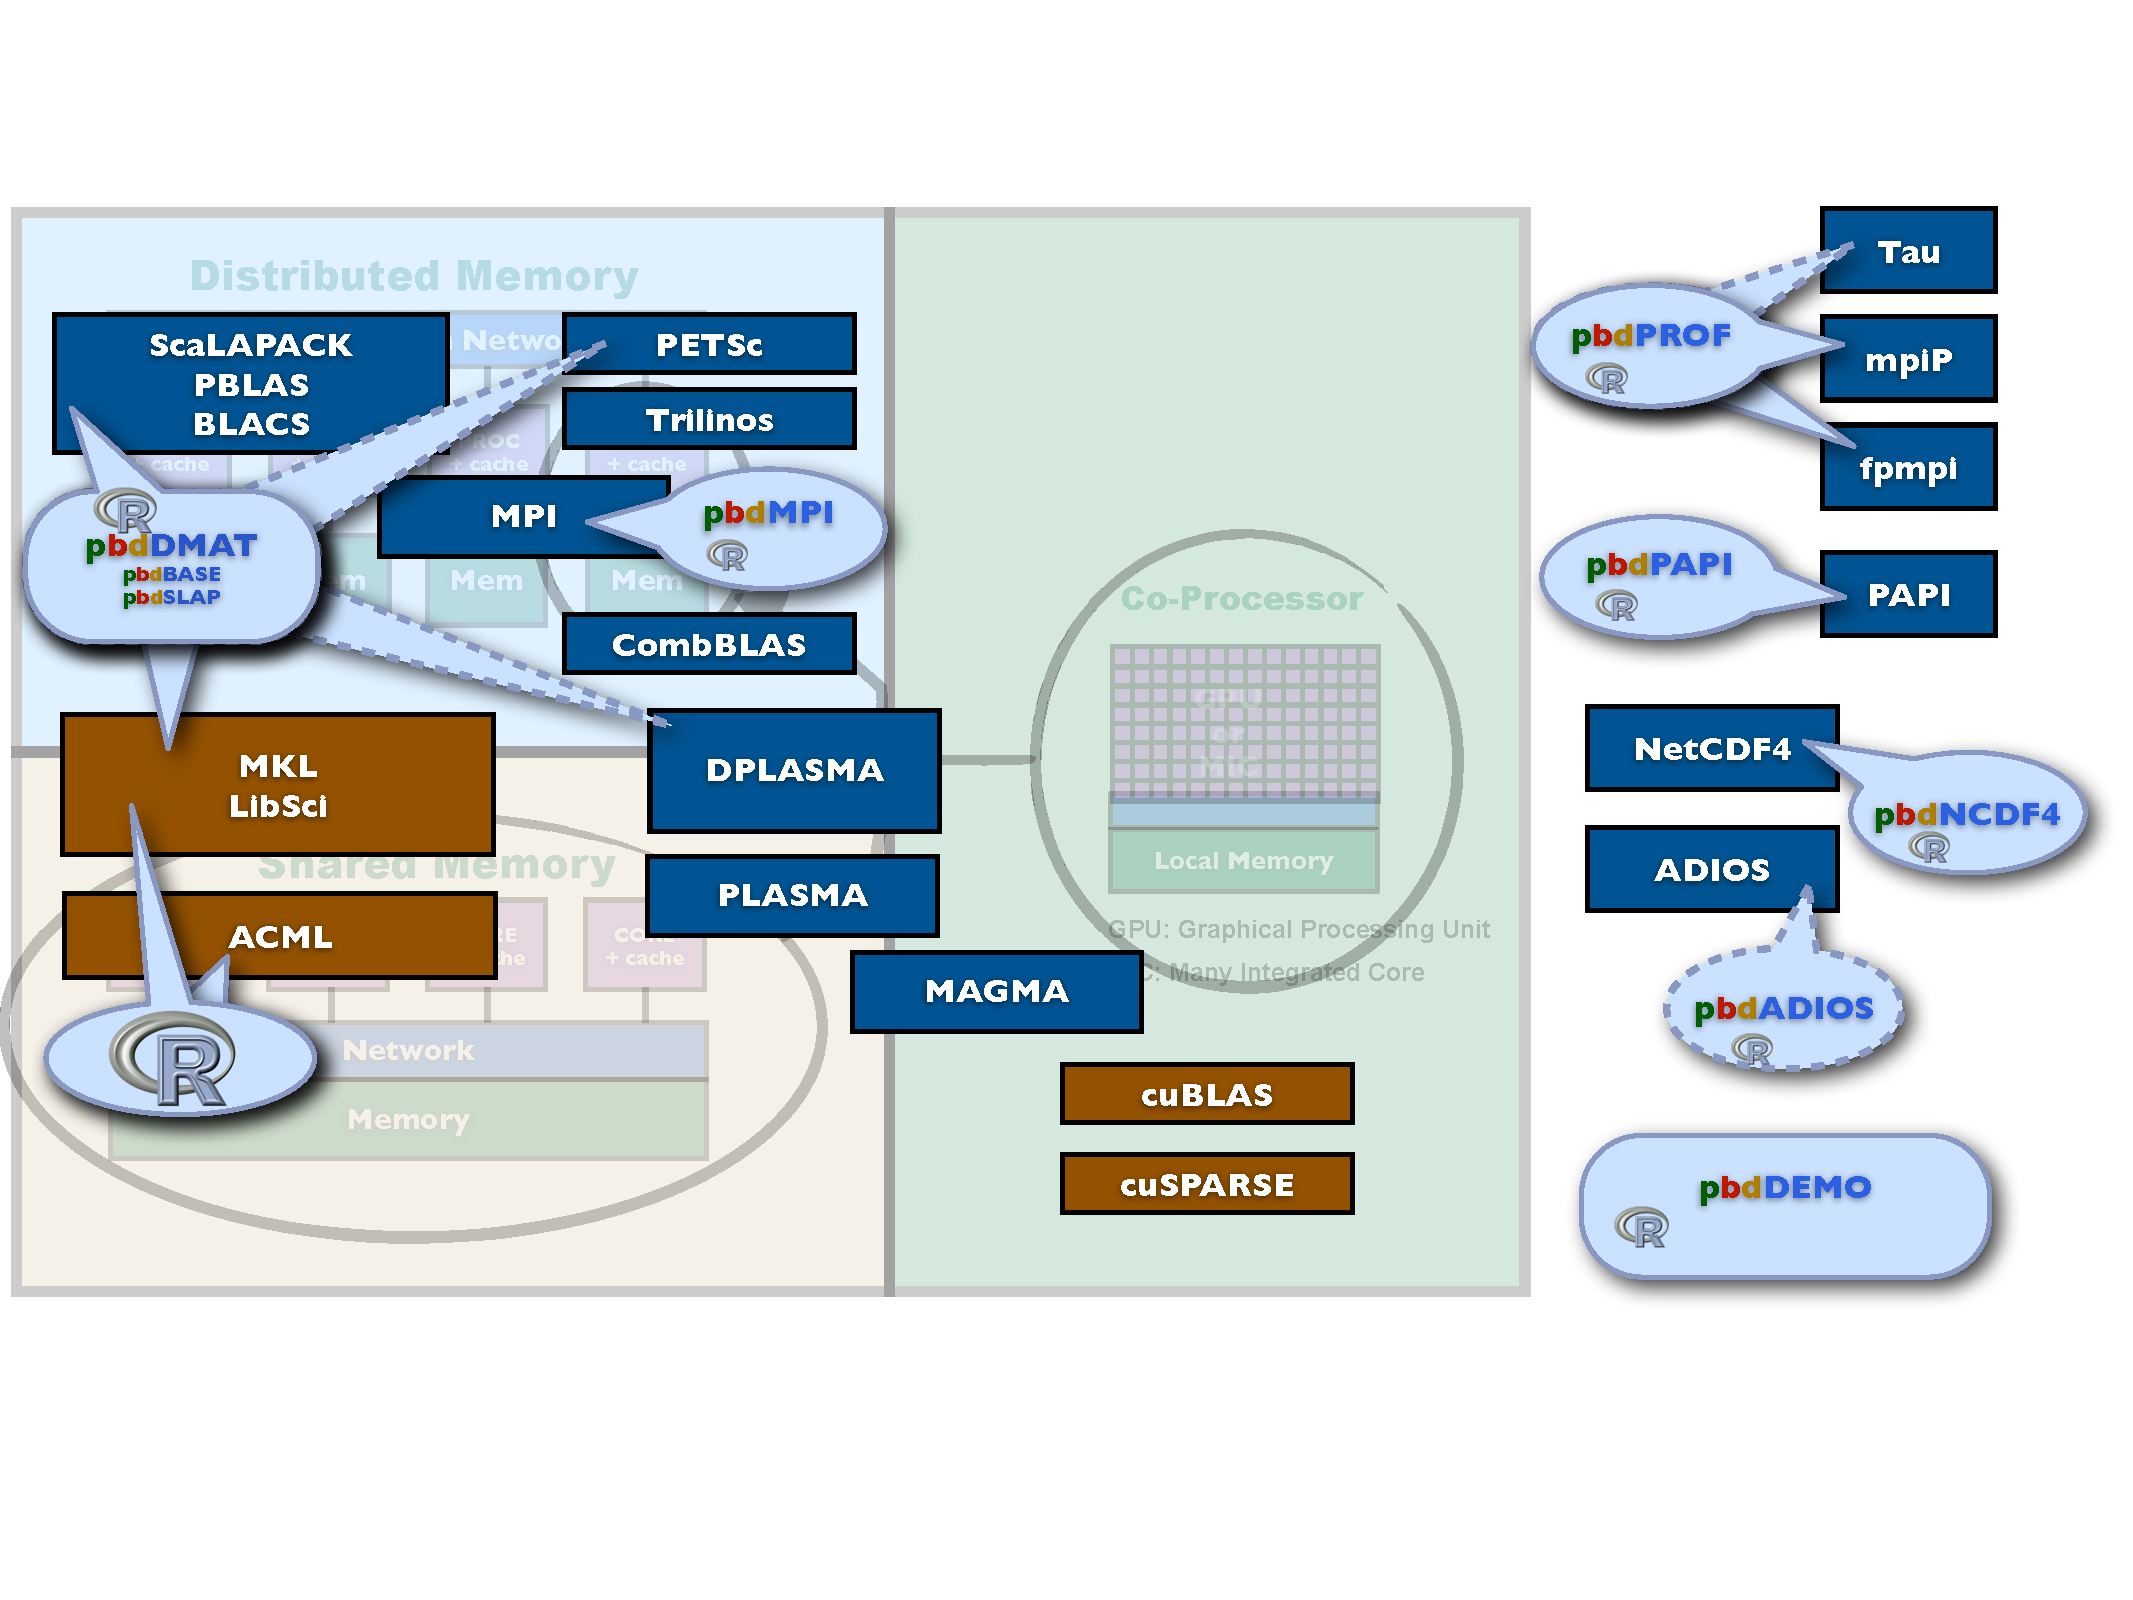
\includegraphics[trim=0cm 5cm 0cm 3cm,clip=true,width=0.85\textwidth]
  {../common/pics/hardware/ParallelHardware27.pdf}
  \scriptsize
  \begin{block}{Why use HPC libraries?}
    \begin{itemize}[<+-|alert@+>]
    \item The HPC community is 30 years beyond ``embarrassingly parallel.''
    \item \emph{They're tested.} \emph{They're
        fast.}  \emph{They're scalable.}
    \item Many science communities are invested in their API.
    \item Data analysis uses much of the same math as simulation science.
    \end{itemize}
  \end{block}
\end{frame}

\subsection{pbdMPI}
\makesubcontentsslidessec

\begin{frame}
  \begin{block}{pbdMPI: a High Level Interface to MPI}
    \begin{itemize}
    \item API is simplified: defaults in control objects.
    \item S4 methods: extensible to complex \R objects.
    \item Additional error checking
    \item Array and matrix methods without serialization: faster than
      \pkg{Rmpi}.
    \end{itemize}
    \begin{center}
      \vspace{0.2cm}\scriptsize
      \begin{tabular}{ll} \hline\hline
        \pkg{pbdMPI} (S4) & \pkg{Rmpi}                \\ \hline
        \code{\color{blue}allreduce}    & \code{mpi.allreduce}      \\
        \code{\color{blue}allgather}    & \code{mpi.allgather},
        \code{mpi.allgatherv},
        \code{mpi.allgather.Robj} \\
        \code{bcast}        & \code{mpi.bcast},
        \code{mpi.bcast.Robj}     \\
        \code{gather}       & \code{mpi.gather},
        \code{mpi.gatherv},
        \code{mpi.gather.Robj}    \\
        \code{recv}         & \code{mpi.recv},
        \code{mpi.recv.Robj}      \\
        \code{reduce}       & \code{mpi.reduce}         \\
        \code{scatter}      & \code{mpi.scatter},
        \code{mpi.scatterv},
        \code{mpi.scatter.Robj}   \\
        \code{send}         & \code{mpi.send},
        \code{mpi.send.Robj}      \\ \hline \hline
      \end{tabular}
    \end{center}
  \end{block}
\end{frame}

\begin{frame}[fragile]
  \begin{block}{Integer?\qquad Not always obvious in R.}
    \vspace{-.2cm}
    \begin{lstlisting}
> is.integer(1)
[1] FALSE
> is.integer(2)
[1] FALSE
> is.integer(1:2)
[1] TRUE
    \end{lstlisting}
  \end{block}
  \begin{block}{Often it's best to let the machine figure it out}\pause
    \begin{minipage}[t]{.475\textwidth}
      \begin{lstlisting}[title=Rmpi]
# int
mpi.allreduce(x, type=1)
# double
mpi.allreduce(x, type=2)
      \end{lstlisting}
    \end{minipage}
    \hfill
    \begin{minipage}[t]{.475\textwidth}
      \begin{lstlisting}[title=pbdMPI]
allreduce(x)
      \end{lstlisting}
      % \vspace{1em}
      % \hspace{1em}{\small S4. Batch only! (No spawning)}
    \end{minipage}
  \end{block}
\end{frame}



% \begin{frame}[fragile,shrink]
%   \begin{block}{Embarrassingly Parallel Computation}\pause
%     \vspace{-1ex}
%     \begin{minipage}[t]{.45\textwidth}
%       \begin{lstlisting}[title=EPforeach.R "asking for parallel",basicstyle=\tiny]
% library(doMPI, quiet=TRUE)
% cl <- startMPIcluster()
% registerDoMPI(cl)

% n <- 10
% myIn <- vector("list", n)

% myFun <- function(x) {
%   s <- sum(rnorm(10000))
%   rank <- mpi.comm.rank(comm=0)
%   return(paste(s, "from", rank))
% }

% results <- foreach(i = 1:n) %dopar% {
%   out <- myFun(myIn[[i]])
% }

% print(results)

% closeCluster(cl)
% mpi.quit()
%       \end{lstlisting}
%     \end{minipage}
%     \hfill
%     \begin{minipage}[t]{.5\textwidth}
%       \begin{lstlisting}[title=EPpbdR.R "thinking parallel",basicstyle=\tiny]
% library(pbdMPI, quiet=TRUE)
% init()

% myChunk <- get.jid(n <- 10)
% myIn <- vector("list", length(myChunk))
% myOut <- vector("list", length(myChunk))

% myFun = function(x) {
%   s <- sum(rnorm(10000))
%   rank <- comm.rank()
%   return(paste(s, "from", rank))
% }

% for(i in 1:length(myChunk)) {
%   myOut[[i]] <- myFun(myIn[[i]])
% }
% results <- gather(myOut)

% comm.print(results)
% finalize()
%       \end{lstlisting}
%     \end{minipage}
%   \end{block}
% \end{frame}


\begin{frame}[fragile]{SPMD Runs Many Copies of One Code}
  \begin{exampleblock}{SPMD Hello World: a ``map-reduce'' to all}
    \vspace{-1.5ex}
    \centering
    \begin{lstlisting}[title=map-reduce.r]
library(pbdMPI, quiet = TRUE)
init()

## Your "Map" code
n <- comm.rank() + 1

## Now "Reduce" but give the result to all
all_sum <- allreduce(n) # Sum is default

text <- paste("Hello: n is", n, "sum is", all_sum )
comm.print(text, all.rank=TRUE)

finalize()
    \end{lstlisting}
    \vspace{-4.5ex}
    \begin{columns}[t,onlytextwidth]
      \begin{column}{0.54\textwidth}
        \begin{lstlisting}[backgroundcolor=\color{white},keywordstyle=\color{black},
title=Execute this batch script via:]
mpirun -np 2 Rscript map-reduce.r
        \end{lstlisting}
      \end{column}
      \hfill
      \begin{column}{0.46\textwidth}
        \begin{lstlisting}[title=Output:]
COMM.RANK = 0
[1] "Hello: n is 1 sum is 3"
COMM.RANK = 1
[1] "Hello: n is 2 sum is 3"
        \end{lstlisting}
      \end{column}
    \end{columns}
  \end{exampleblock}
\end{frame}

\subsection{pbdDMAT}
\makesubcontentsslidessec

\begin{frame}{Dense Matrix and Vector Operations}
  \begin{block}{A matrix is mapped to a processor grid shape}
    \begin{table}[ht]
      \centering
      % \begin{subfigure}[b]{0.23\textwidth}
      %   \centering
      %   $\left[\begin{tabular}{l}
      %       0 \\ 1 \\ 2 \\ 3 \\ 4 \\ 5
      %     \end{tabular}\right]^T$
      %   \caption{$1\times 6$}
      % \end{subfigure}
      \begin{subfigure}[b]{0.23\textwidth}
        \centering
        $\left[\begin{tabular}{llllll}
            0 & 1 & 2 & 3 & 4 & 5
          \end{tabular}\right]$
        \vspace{1.5cm}
        \caption{$1\times 6$}
      \end{subfigure}%\hspace{-1cm}
      \begin{subfigure}[b]{0.23\textwidth}
        \centering
        $\left[\begin{tabular}{lll}
            0 & 1 & 2\\
            3 & 4 & 5
          \end{tabular}\right]$
        \caption{$2\times 3$}
      \end{subfigure}%
      \begin{subfigure}[b]{0.23\textwidth}
        \centering
        $\left[\begin{tabular}{ll}
            0 & 1 \\
            2 & 3\\
            4 & 5
          \end{tabular}\right]$
        \caption{$3\times 2$}
      \end{subfigure}
      \begin{subfigure}[b]{0.23\textwidth}
        \centering
        $\left[\begin{tabular}{l}
            0 \\ 1 \\ 2 \\ 3 \\ 4 \\ 5
          \end{tabular}\right]$
        \caption{$6\times 1$}
      \end{subfigure}
      \caption{Processor Grid Shapes with 6 Processors}\label{fig:gridshapes}
    \end{table}
  \end{block}
\end{frame}

\begin{frame}[shrink]
\begin{exampleblock}{2$\times$3 block-cyclic grid on 6 processors:
    Global view ``ddmatrix'' class}
\begin{align*}
x &= \left[
      \begin{array}{ll|ll|ll|ll|l}
      \color{g11}x_{11} & \color{g11}x_{12} & \color{g12}x_{13} & \color{g12}x_{14} & \color{g13}x_{15} & \color{g13}x_{16} & \color{g11}x_{17} & \color{g11}x_{18} & \color{g12}x_{19}\\
      \color{g11}x_{21} & \color{g11}x_{22} & \color{g12}x_{23} & \color{g12}x_{24} & \color{g13}x_{25} & \color{g13}x_{26} & \color{g11}x_{27} & \color{g11}x_{28} & \color{g12}x_{29}\\\hline
      \color{g21}x_{31} & \color{g21}x_{32} & \color{g22}x_{33} & \color{g22}x_{34} & \color{g23}x_{35} & \color{g23}x_{36} & \color{g21}x_{37} & \color{g21}x_{38} & \color{g22}x_{39}\\
      \color{g21}x_{41} & \color{g21}x_{42} & \color{g22}x_{43} & \color{g22}x_{44} & \color{g23}x_{45} & \color{g23}x_{46} & \color{g21}x_{47} & \color{g21}x_{48} & \color{g22}x_{49}\\\hline
      \color{g11}x_{51} & \color{g11}x_{52} & \color{g12}x_{53} & \color{g12}x_{54} & \color{g13}x_{55} & \color{g13}x_{56} & \color{g11}x_{57} & \color{g11}x_{58} & \color{g12}x_{59}\\
      \color{g11}x_{61} & \color{g11}x_{62} & \color{g12}x_{63} & \color{g12}x_{64} & \color{g13}x_{65} & \color{g13}x_{66} & \color{g11}x_{67} & \color{g11}x_{68} & \color{g12}x_{69}\\\hline
      \color{g21}x_{71} & \color{g21}x_{72} & \color{g22}x_{73} & \color{g22}x_{74} & \color{g23}x_{75} & \color{g23}x_{76} & \color{g21}x_{77} & \color{g21}x_{78} & \color{g22}x_{79}\\
      \color{g21}x_{81} & \color{g21}x_{82} & \color{g22}x_{83} & \color{g22}x_{84} & \color{g23}x_{85} & \color{g23}x_{86} & \color{g21}x_{87} & \color{g21}x_{88} & \color{g22}x_{89}\\\hline
      \color{g11}x_{91} & \color{g11}x_{92} & \color{g12}x_{93} & \color{g12}x_{94} & \color{g13}x_{95} & \color{g13}x_{96} & \color{g11}x_{97} & \color{g11}x_{98} & \color{g12}x_{99}\\
      \end{array}
\right]_{9\times 9}
\end{align*}
\begin{align*}
\text{Processor grid = }\left|
      \begin{array}{lll}
      \color{g11}0 & \color{g12}1 & \color{g13}2\\
      \color{g21}3 & \color{g22}4 & \color{g23}5
      \end{array}
\right| &=
\left|
      \begin{tabular}{lll}
      \color{g11}(0,0) & \color{g12}(0,1) & \color{g13}(0,2)\\
      \color{g21}(1,0) & \color{g22}(1,1) & \color{g23}(1,2)
      \end{tabular}
\right|
\end{align*}
\end{exampleblock}
\end{frame}


\begin{frame}[shrink]
\begin{exampleblock}{2$\times$3 block-cyclic grid on 6 processors:
    Local view ``ddmatrix'' class}
\begin{align*}
\left[
      \begin{array}{ll|ll}
      \color{g11}x_{11} & \color{g11}x_{12} & \color{g11}x_{17} & \color{g11}x_{18}\\
      \color{g11}x_{21} & \color{g11}x_{22} & \color{g11}x_{27} & \color{g11}x_{28}\\\hline
      \color{g11}x_{51} & \color{g11}x_{52} & \color{g11}x_{57} & \color{g11}x_{58}\\
      \color{g11}x_{61} & \color{g11}x_{62} & \color{g11}x_{67} & \color{g11}x_{68}\\\hline
      \color{g11}x_{91} & \color{g11}x_{92} & \color{g11}x_{97} & \color{g11}x_{98}\\
      \end{array}
\right]_{5\times 4}
\left[
      \begin{array}{ll|l}
      \color{g12}x_{13} & \color{g12}x_{14} & \color{g12}x_{19}\\
      \color{g12}x_{23} & \color{g12}x_{24} & \color{g12}x_{29}\\\hline
      \color{g12}x_{53} & \color{g12}x_{54} & \color{g12}x_{59}\\
      \color{g12}x_{63} & \color{g12}x_{64} & \color{g12}x_{69}\\\hline
      \color{g12}x_{93} & \color{g12}x_{94} & \color{g12}x_{99}\\
      \end{array}
\right]_{5\times 3}
\left[
      \begin{array}{ll}
      \color{g13}x_{15} & \color{g13}x_{16}\\
      \color{g13}x_{25} & \color{g13}x_{26}\\\hline
      \color{g13}x_{55} & \color{g13}x_{56}\\
      \color{g13}x_{65} & \color{g13}x_{66}\\\hline
      \color{g13}x_{95} & \color{g13}x_{96}\\
      \end{array}
\right]_{5\times 2}
\\
\left[
      \begin{array}{ll|ll}
      \color{g21}x_{31} & \color{g21}x_{32} & \color{g21}x_{37} & \color{g21}x_{38}\\
      \color{g21}x_{41} & \color{g21}x_{42} & \color{g21}x_{47} & \color{g21}x_{48}\\\hline
      \color{g21}x_{71} & \color{g21}x_{72} & \color{g21}x_{77} & \color{g21}x_{78}\\
      \color{g21}x_{81} & \color{g21}x_{82} & \color{g21}x_{87} & \color{g21}x_{88}\\
      \end{array}
\right]_{4\times 4}
\left[
      \begin{array}{ll|l}
      \color{g22}x_{33} & \color{g22}x_{34} & \color{g22}x_{39}\\
      \color{g22}x_{43} & \color{g22}x_{44} & \color{g22}x_{49}\\\hline
      \color{g22}x_{73} & \color{g22}x_{74} & \color{g22}x_{79}\\
      \color{g22}x_{83} & \color{g22}x_{84} & \color{g22}x_{89}\\
      \end{array}
\right]_{4\times 3}
\left[
      \begin{array}{ll}
      \color{g23}x_{35} & \color{g23}x_{36} \\
      \color{g23}x_{45} & \color{g23}x_{46} \\\hline
      \color{g23}x_{75} & \color{g23}x_{76} \\
      \color{g23}x_{85} & \color{g23}x_{86} \\
      \end{array}
\right]_{4\times 2}
\end{align*}
\begin{align*}
\text{Processor grid = }\left|
      \begin{array}{lll}
      \color{g11}0 & \color{g12}1 & \color{g13}2\\
      \color{g21}3 & \color{g22}4 & \color{g23}5
      \end{array}
\right| &=
\left|
      \begin{tabular}{lll}
      \color{g11}(0,0) & \color{g12}(0,1) & \color{g13}(0,2)\\
      \color{g21}(1,0) & \color{g22}(1,1) & \color{g23}(1,2)
      \end{tabular}
\right|
\end{align*}
\end{exampleblock}
\end{frame}

\begin{frame}[fragile]
  \begin{block}{\pbdR\ No change in syntax. \hfill Data redistribution functions.}
\vspace{-2ex}
  \begin{lstlisting}
x <- x[-1, 2:5]
x <- log(abs(x) + 1)
x.pca <- prcomp(x)
xtx <- t(x) %*% x
ans <- svd(solve(xtx))
  \end{lstlisting}
\vspace{-1ex}
  \begin{center}
  \emph{The above (and over 100 other functions) runs on 1 core with R \\
    or 10,000 cores with \pbdR ddmatrix class}
  \end{center}
\vspace{-2ex}
\begin{lstlisting}
> showClass("ddmatrix")
Class "ddmatrix" [package "pbdDMAT"]
Slots:
Name:     Data     dim    ldim   bldim   ICTXT
Class:  matrix numeric numeric numeric numeric
\end{lstlisting}
\vspace{-2ex}
\begin{lstlisting}
> x <- as.rowblock(x)
> x <- as.colblock(x)
> x <- redistribute(x, bldim=c(8, 8), ICTXT = 0)
\end{lstlisting}
  \end{block}
\end{frame}

\input{../common/06_dmatstats/randsvd.tex}



\section{Benchmarks}

\hidenum
\begin{frame}[noframenumbering]
\frametitle{Contents}
 \tableofcontents[currentsection,hideallsubsections]
\end{frame}
\shownum

\subsection{Productivity Benchmark}

\begin{frame}[fragile]
\fontsize{8pt}{10}\selectfont
\begin{block}{Truncated SVD from Random Projections\footnotemark}
  \begin{minipage}{.55\textwidth}
    \begin{center}
      \includegraphics[width=.95\textwidth]{../common/pics/randSVDalg}
      \\
      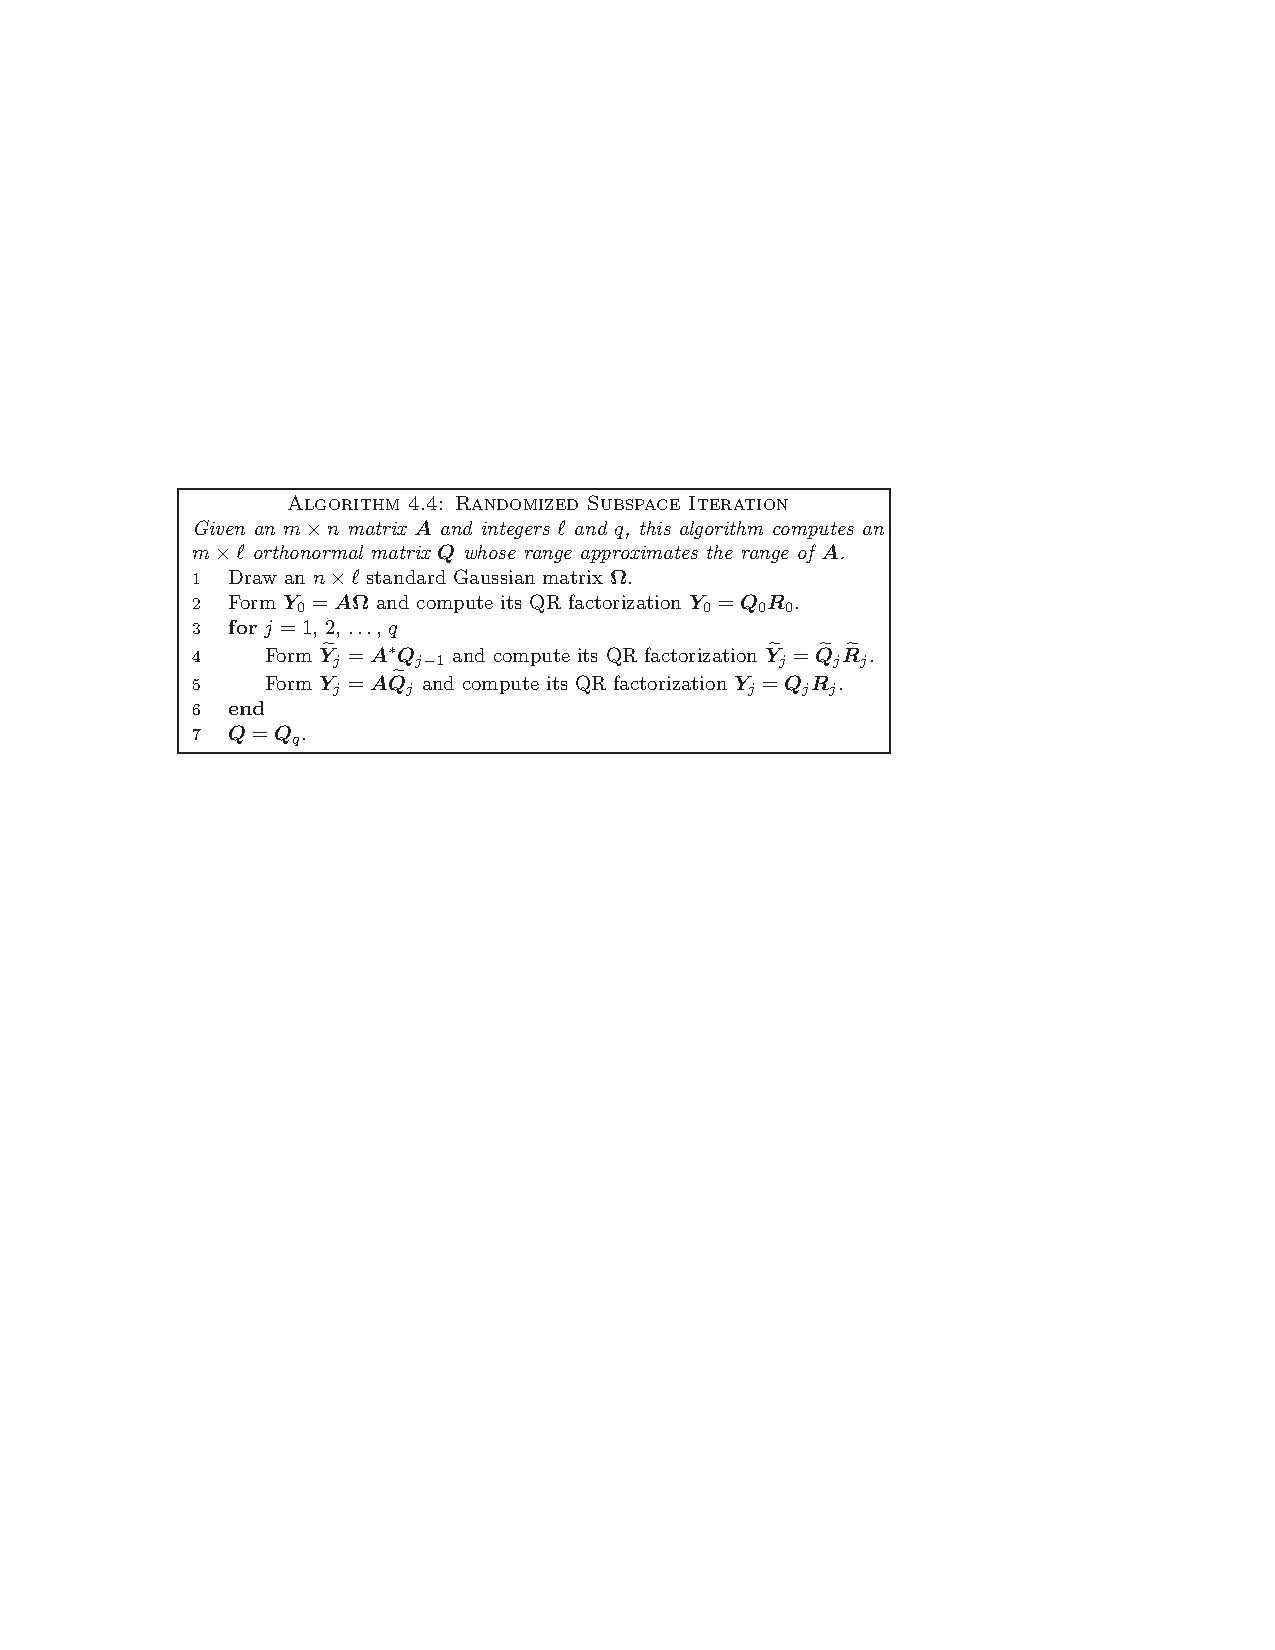
\includegraphics[width=.95\textwidth]{../common/pics/randSVDalg4_4}
    \end{center}
  \end{minipage}
%   \hspace{.01cm}
  \begin{minipage}{0.430\textwidth}
\begin{lstlisting}[title=Serial 
R,basicstyle=\tiny,backgroundcolor=\color{grayish} 
,numberstyle=\tiny\color{black},keywordstyle=\color{black},commentstyle=\color{ 
dkgreen},stringstyle=\color{black},escapeinside={(*@}{@*)}]
randSVD <- function(A, k, q=3)
  {
    ## Stage A
    Omega <- (*@ matrix(rnorm(n*2*k),@*) 
            (*@ nrow=n, ncol=2*k) @*)
    Y <- A %*% Omega
    Q <- qr.Q(qr(Y))
    At <- t(A)
    for(i in 1:q)
      {
        Y <- At %*% Q
        Q <- qr.Q(qr(Y))
        Y <- A %*% Q
        Q <- qr.Q(qr(Y))
      }
    
    ## Stage B
    B <- t(Q) %*% A
    U <- La.svd(B)$u
    U <- Q %*% U
    U[, 1:k]
  }
\end{lstlisting} %balance$
\end{minipage}
{\fontsize{6pt}{10}\selectfont $^1$Halko, Martinsson, 
  and Tropp, 2011. Finding structure with randomness: probabilistic algorithms 
  for constructing approximate matrix decompositions \emph{SIAM Review} \textbf{53} 
  217--288}
\end{block}
\end{frame}


\begin{frame}[fragile]
 \fontsize{8pt}{10}\selectfont
\begin{block}{Randomized SVD}
  \hfill
  \begin{minipage}{0.430\textwidth}
\begin{lstlisting}[title=Serial 
R,basicstyle=\tiny,backgroundcolor=\color{grayish} 
,numberstyle=\tiny\color{black},keywordstyle=\color{black},commentstyle=\color{ 
dkgreen},stringstyle=\color{black},escapeinside={(*@}{@*)}]
randSVD <- function(A, k, q=3)
  {
    ## Stage A
    Omega <- (*@ \textcolor{blue}{matrix(rnorm(n*2*k),} @*) 
         (*@ \textcolor{blue}{ nrow=n, ncol=2*k)} @*)
    Y <- A %*% Omega
    Q <- qr.Q(qr(Y))
    At <- t(A)
    for(i in 1:q)
      {
        Y <- At %*% Q
        Q <- qr.Q(qr(Y))
        Y <- A %*% Q
        Q <- qr.Q(qr(Y))
      }
    
    ## Stage B
    B <- t(Q) %*% A
    U <- La.svd(B)$u
    U <- Q %*% U
    U[, 1:k]
  }
\end{lstlisting} %balance$
  \end{minipage}
  \hfill
  \begin{minipage}{0.430\textwidth}
\begin{lstlisting}[title=Parallel pbdR,basicstyle=\tiny,backgroundcolor=\color{
grayish}, numberstyle=\tiny\color{black},keywordstyle=\color{black},
commentstyle=\color{dkgreen},stringstyle=\color{black},escapeinside={(*@}{@*)}]
randSVD <- function(A, k, q=3)
  {
    ## Stage A
    Omega <- (*@ \textcolor{blue}{ddmatrix("rnorm",} @*)
         (*@ \textcolor{blue}{nrow=n, ncol=2*k)} @*)
    Y <- A %*% Omega
    Q <- qr.Q(qr(Y))
    At <- t(A)      
    for(i in 1:q)
      {
        Y <- At %*% Q   
        Q <- qr.Q(qr(Y))
        Y <- A %*% Q    
        Q <- qr.Q(qr(Y))
      }
    
    ## Stage B
    B <- t(Q) %*% A     
    U <- La.svd(B)$u 
    U <- Q %*% U     
    U[, 1:k]
  }
\end{lstlisting}  % balancing $
  \end{minipage}
\hfill
\end{block}
\end{frame}

\begin{frame}
  \begin{block}{Randomized SVD}
    \begin{center}
      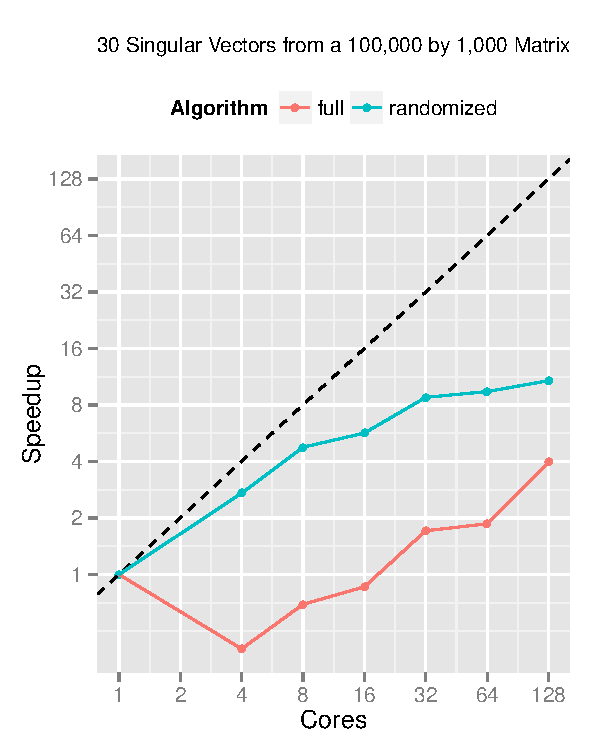
\includegraphics[width=.45\textwidth]{../common/pics/randSVDspeedup}
      \hfill
      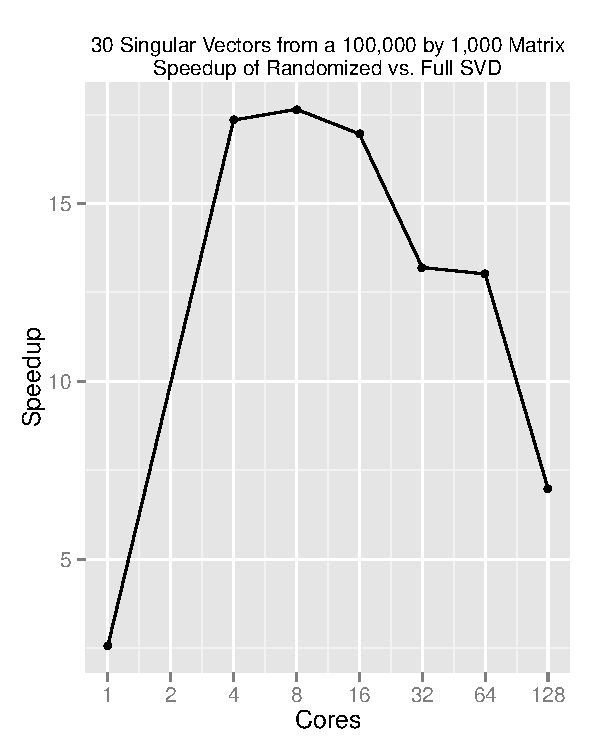
\includegraphics[width=.45\textwidth]{../common/pics/randSpeedupSVD}
    \end{center}
  \end{block}
\end{frame}

\subsection{Scalability Benchmarks}

\begin{frame}
  \begin{block}{Non-Optimal Choices Throughout}
    \begin{enumerate}[<+-|alert@+>]
      \item Only libre software used (no MKL, ACML, etc.).
      \item 1 core = 1 MPI process.
      \item No tuning for data layout.
    \end{enumerate}
  \end{block}
  \begin{block}{Benchmark Data}
    \begin{enumerate}[<+-|alert@+>]
      \item Random normal $N(100, 10000)$.
      \item Local problem size of $\approx 45.5 MB$.
      \item Three sets:  500, 1000, and 2000 columns.
      \item Several runs at different core sizes within each set.
    \end{enumerate}
  \end{block}
\end{frame}



% \subsection{Covariance}

\begin{frame}[fragile]
  \begin{block}{Covariance Code}
\begin{lstlisting}
x <- ddmatrix("rnorm", nrow=n, ncol=p, mean=mean, sd=sd)

cov.x <- cov(x)
\end{lstlisting}
  \end{block}
\end{frame}

\begin{frame}
  \begin{block}{\code{cov()}}
  \begin{center}
    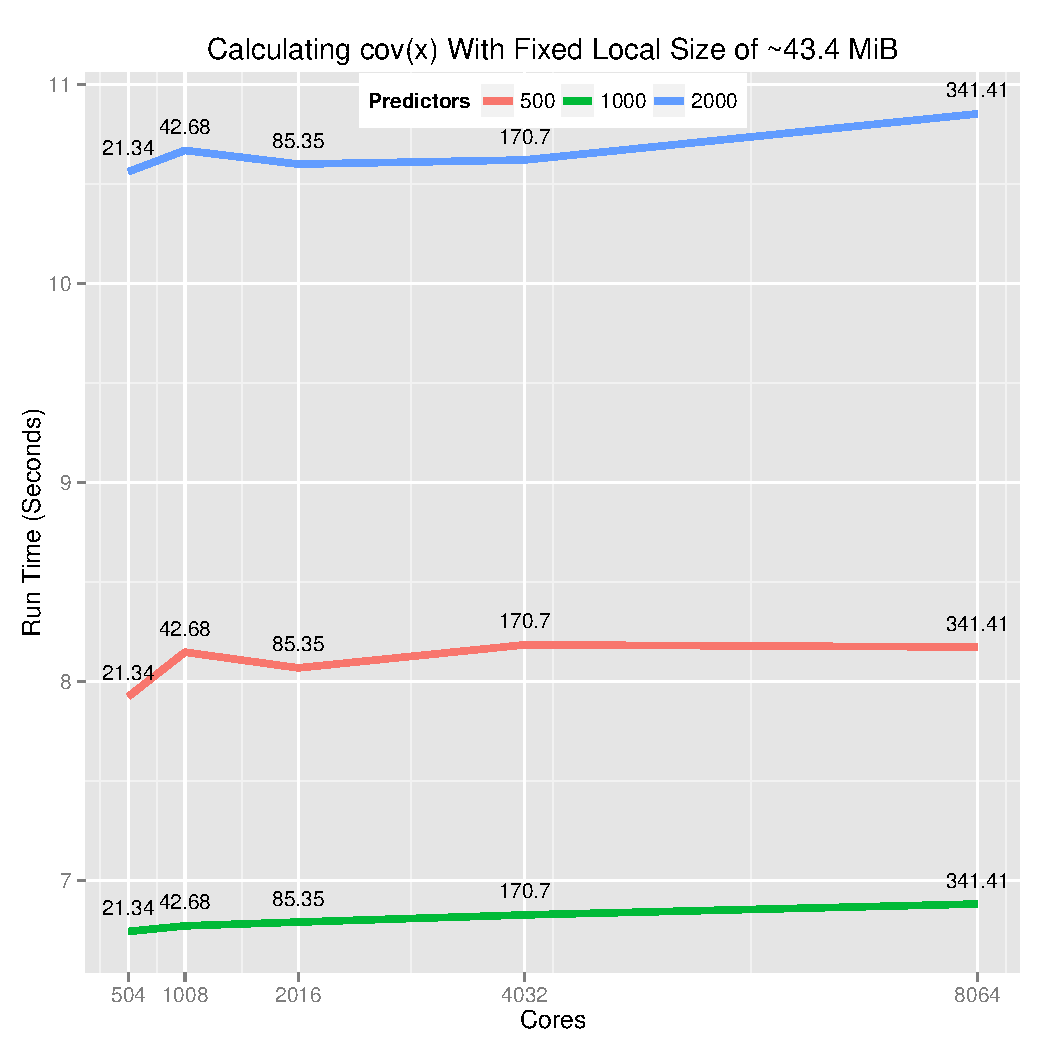
\includegraphics[height=.88\textheight]{../common/pics/cov}
  \end{center}
  \end{block}
\end{frame}



% \subsection{Linear Model Fitting}

\begin{frame}[fragile]
  \begin{block}{Linear Model Code}
\begin{lstlisting}
x <- ddmatrix("rnorm", nrow=n, ncol=p, mean=mean, sd=sd)
beta_true <- ddmatrix("runif", nrow=p, ncol=1)

y <- x %*% beta_true

beta_est <- lm.fit(x=x, y=y)$coefficients 
\end{lstlisting}
  \end{block}
\end{frame}

\begin{frame}
  \begin{block}{\code{Data Generation}}
  \begin{center}
    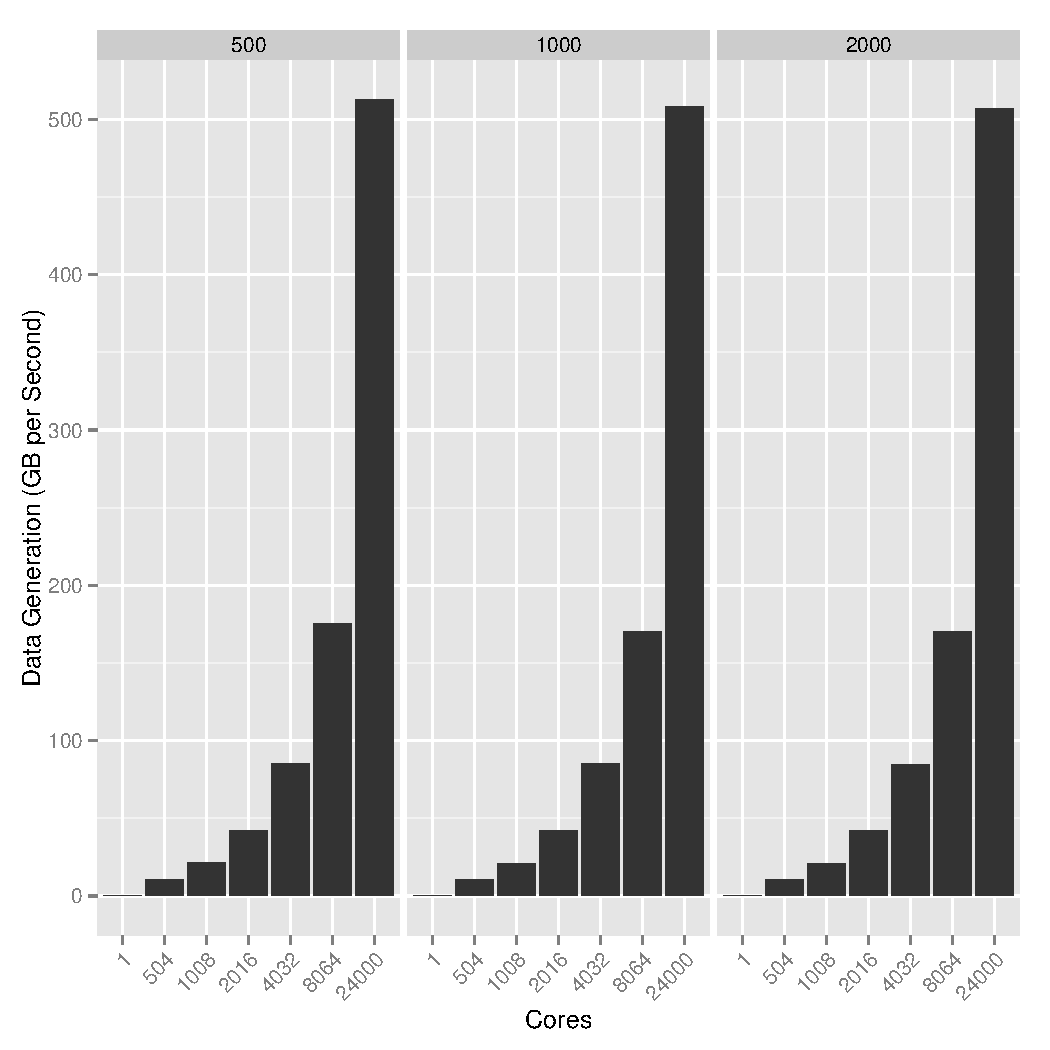
\includegraphics[height=.88\textheight]{../common/pics/datagen}
  \end{center}
  \end{block}
\end{frame}

% \begin{frame}
%   \begin{block}{\code{lm.fit()}}
%   \begin{center}
%     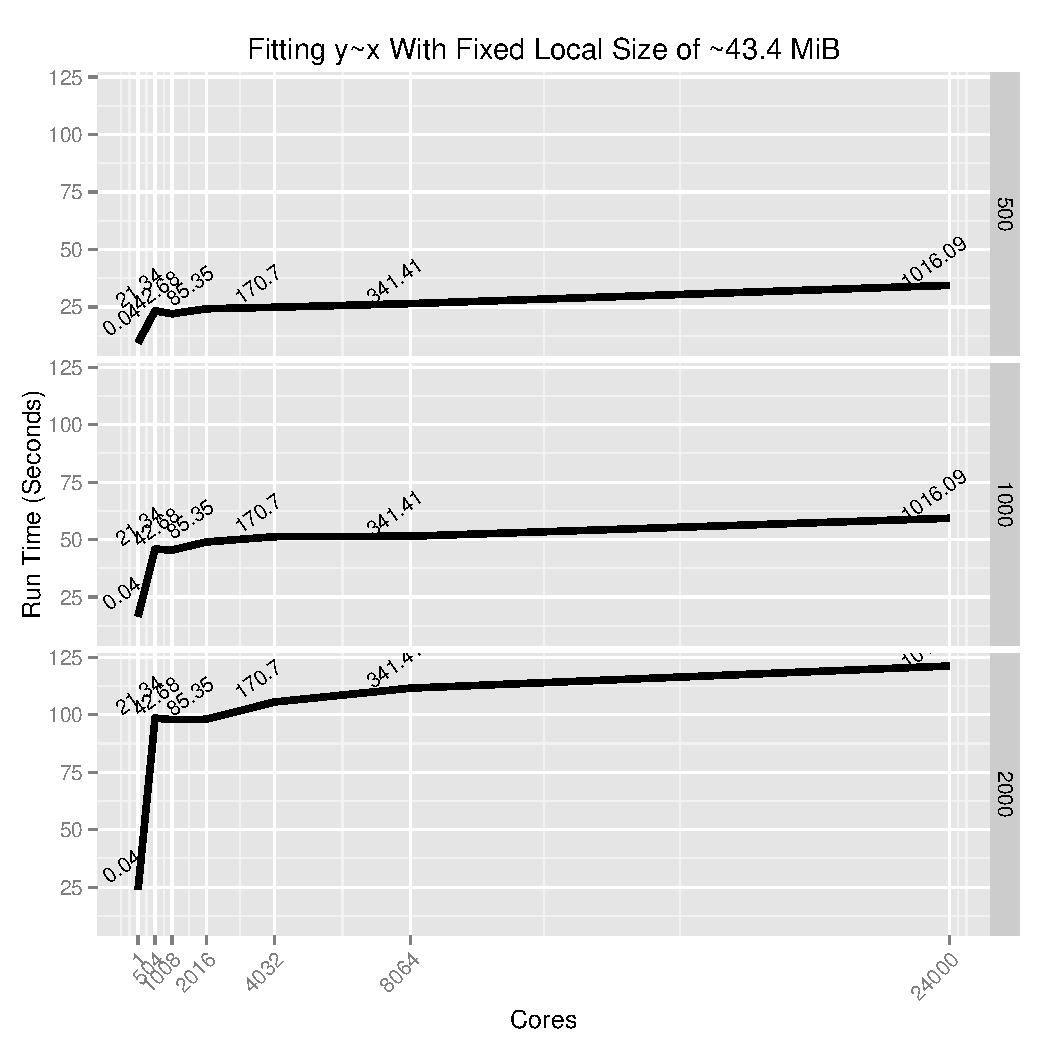
\includegraphics[height=.88\textheight]{../common/pics/lmfit1}
%   \end{center}
%   \end{block}
% \end{frame}

\begin{frame}
  \begin{block}{\code{lm.fit()}}
  \begin{center}
    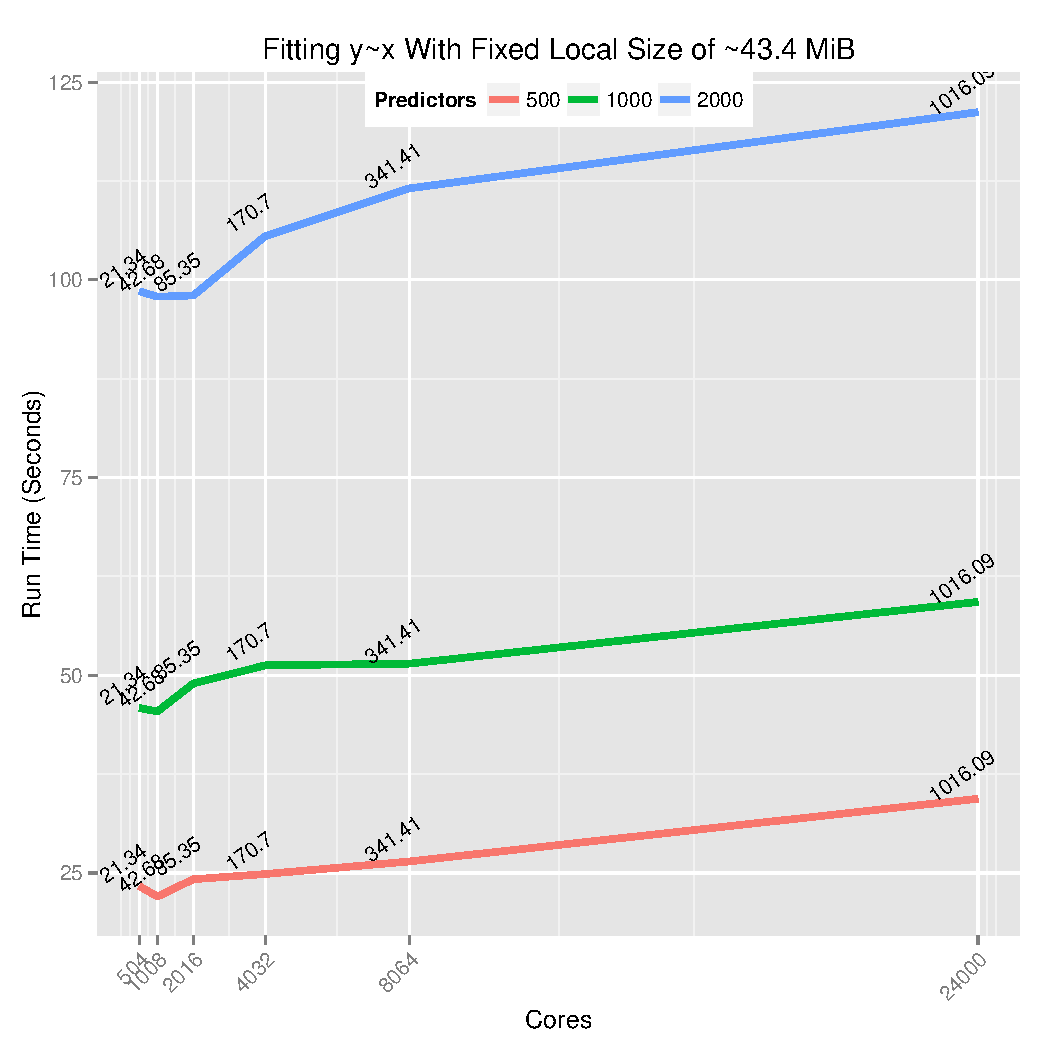
\includegraphics[height=.88\textheight]{../common/pics/lmfit2}
  \end{center}
  \end{block}
\end{frame}
\section{Challenges}

\hidenum
\begin{frame}[noframenumbering]
\frametitle{Contents}
 \tableofcontents[currentsection,hideallsubsections]
\end{frame}
\shownum


\subsection{Challenges}

\begin{frame}
  \begin{block}{Challenges}
    \begin{itemize}[<+-|alert@+>]
      \item Perceptions.
      \item Library loading.
      \item Profiling.
    \end{itemize}
  \end{block}
\end{frame}


\begin{frame}
  \begin{block}{Covariance Revisited: Distributed Data Parameter Calibration}
    \begin{center}
     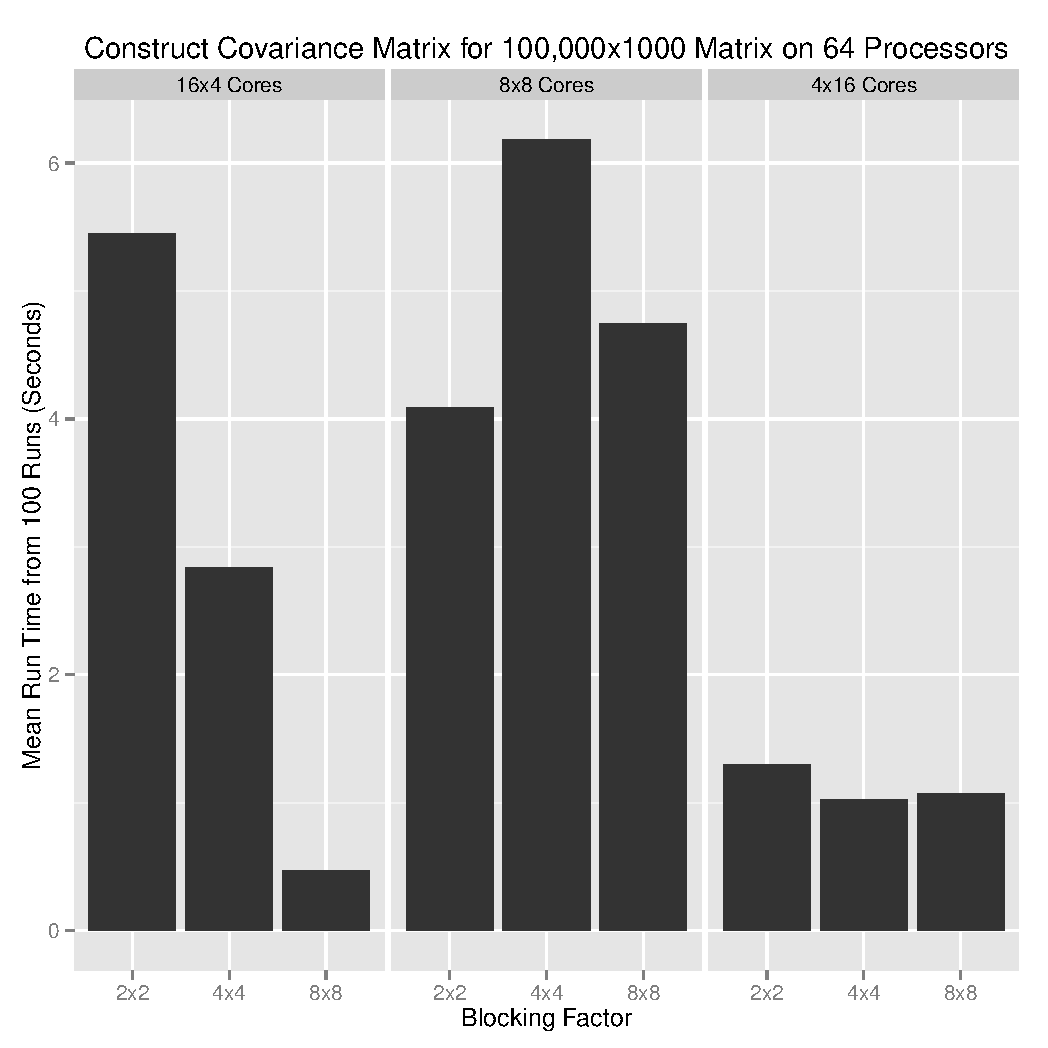
\includegraphics[width=10cm, height=7cm]{../common/pics/cov_param}
    \end{center}
  \end{block}
\end{frame}

\begin{frame}
  \begin{block}{Adding More Levels of Parallelism}
    \begin{center}
      {\color{dkblue}Distributed Memory (cluster nodes)} \\
      {\color{dkgreen}Shared Memory (multicore)} \\
      {\color{purple}Co-Processor (GPU, manycore)}
    \end{center}
    \begin{itemize}
      \item {\color{dkblue}pbdDMAT} + {\color{purple}CUBLAS}: near term on Titan 
      \item {\color{dkblue}pbdDMAT} - {\color{dkblue}ScaLAPACK} +
        {\color{dkblue}D}{\color{dkgreen}PLASMA}: QR only 
      \item {\color{dkblue}pbdDMAT} + {\color{dkgreen}PLASMA} or
        {\color{dkgreen}MKL} or {\color{dkgreen}ACML}: often helps 
      \item {\color{dkblue}pbdDMAT} + {\color{purple}MAGMA}: may not help 
    \end{itemize}
  \end{block}
\end{frame}

\hidenum
\section*{}
\begin{frame}[noframenumbering]
  \begin{block}{Tutorials}
  \begin{itemize}
    \item {\small OLCF Very Large Data Workshop
         ... {\color{red} NEXT!}}
    \item {\small Seoul National University, August 20}
    \item {\small SC13, November 17-22, Denver}
  \end{itemize}
  \end{block}
  \begin{block}{Invited Talks}
  \begin{itemize}
    \item {\small International Association for Statistical Computing, Aug 22-23, Seoul}
    \item {\small 59th ISI World Statistics Congress, August 25-30, Hong Kong }
  \end{itemize}
  \end{block}
\end{frame}
  
\begin{frame}[noframenumbering]
 \begin{block}{Thanks for coming!}
 \begin{center}
     {\Large Questions?}\\[1cm]
     {\Large Be sure to stick around for the tutorial!}
  \end{center}
 \end{block}
\end{frame}


\end{document}
% -------------------------------------------------------------------------
% Logos
% -------------------------------------------------------------------------

\definecolor{ORNL}{HTML}{008752}
\definecolor{UT}{HTML}{F77F00}
\setbeamercolor{title}{fg=white}
\setbeamercolor{frametitle}{fg=white}


\newcommand{\titlelogos}{}

\newcommand{\utpres}{
\renewcommand*\titlelogos{\centering
\includegraphics[scale=.6]{%
../common/pics/logos/logos_ut}}
  \logo{
\includegraphics[height=.34cm]{../common/pics/logos/utk.png}}
  \setbeamercolor{structure}{fg=UT}
}

\newcommand{\ornlpres}{
\renewcommand*\titlelogos{\centering
\includegraphics[scale=.6]{%
../common/pics/logos/logos_ornl}}
  \logo{
\includegraphics[height=.34cm]{../common/pics/logos/ornl.jpg}}
  \setbeamercolor{structure}{fg=ORNL}
}

\newcommand{\allpres}{
  \renewcommand*\titlelogos{\centering%
  
\includegraphics[scale=.6]{../common/pics/logos/logos_all}}

  \logo{\begin{tabular}{r}\includegraphics[height=.34cm]%
  {../common/pics/logos/utk.png} \\ 
  \includegraphics[height=.34cm]%
  {../common/pics/logos/ornl.jpg}\end{tabular}}
  \setbeamercolor{structure}{fg=UT}
}

\newcommand{\allpresou}{
\renewcommand*\titlelogos{\centering
\includegraphics[scale=.6]{%
../common/pics/logos/logos_all}}
  \logo{\begin{tabular}{r}
\includegraphics[height=.34cm]{%
          ../common/pics/logos/ornl.jpg} \\ 

\includegraphics[height=.34cm]{../common/pics/logos/utk.png}\end{tabular}}
  \setbeamercolor{structure}{fg=ORNL}
}



% -------------------------------------------------------------------------
% Subsection contents slides
% -------------------------------------------------------------------------

\newcommand{\makesubcontentsslides}{
  \hidenum
\begin{frame}[noframenumbering]
\frametitle{Contents}
 \tableofcontents[currentsection,hideothersubsections,sectionstyle=show/hide]
\end{frame}
\shownum
}

\newcommand{\makesubcontentsslidessec}{
  \hidenum
\begin{frame}[noframenumbering]
\tableofcontents[currentsection,
  sectionstyle=show/show,
  subsectionstyle=show/shaded/hide]
\end{frame}
\shownum
}


\usepackage{xcolor}

\definecolor{gray}{rgb}{.6,.6,.6}
\definecolor{orange}{rgb}{1,0.5,0}
\definecolor{grayish}{rgb}{.875, .875, .875}
\definecolor{dkgray}{rgb}{.375, .375, .375}
\definecolor{dkgreen}{rgb}{0,0.6,0}
\definecolor{mauve}{rgb}{0.58,0,0.82}
\definecolor{dkblue}{rgb}{0, 0, .5}

\definecolor{g11}{rgb}{0, 0, 1}
\definecolor{g12}{rgb}{0, .4, 1}
\definecolor{g13}{rgb}{0, .8, 1}

\definecolor{g21}{rgb}{0, .5, .3}
\definecolor{g22}{rgb}{.4, .5, .3}
\definecolor{g23}{rgb}{.8, .5, .3}
\usepackage{listings}

\lstset{ %
  language=R,     
  numbers=left,
  stepnumber=1,       
  numbersep=6pt,      
  showspaces=false,      
  showstringspaces=false,  
  showtabs=false,    
  frame=single,      
  rulecolor=\color{black},   
  tabsize=4,     
  captionpos=t,     
  breaklines=true,     
  breakatwhitespace=true,   
  title=\lstname,              
  basicstyle=\ttfamily\color{black}\scriptsize, 
  backgroundcolor=\color{grayish},  
  numberstyle=\tiny\color{black},  
  keywordstyle=\color{blue}, 
  commentstyle=\color{dkgreen}, 
  stringstyle=\color{mauve}, 
  xleftmargin=.1in,
  xrightmargin=.1in,
  aboveskip=0cm,
  belowskip=.2cm
  %   escapeinside={\%*}{*)},    
%   morekeywords={*,...}    
}


\lstdefinelanguage{shl}{
  language=sh,
  backgroundcolor=\color{white},
  basicstyle=\scriptsize\ttfamily\color{black},
  keywordstyle=\color{blue},
  commentstyle=\color{dkgreen},
  stringstyle=\color{mauve},
  numbers=none
}


\lstdefinelanguage{Rinteractive}{
  language=Sh,
  backgroundcolor=\color{white},
  basicstyle=\scriptsize\ttfamily\color{black},
  keywordstyle=\color{black},
  commentstyle=\color{black},
  stringstyle=\color{black},
  numbers=none
}


\lstdefinelanguage{Rcpp}{
        language=C++,
        basicstyle=\ttfamily\color{black}\scriptsize,
        backgroundcolor=\color{white},
        frame=single,
        breaklines=true,
        keywordstyle=\color{blue},
        commentstyle=\color{dkgreen}\itshape,
        stringstyle=\color{mauve},
        numbers=none,
        showspaces=false,
        showstringspaces=false,
        showtabs=false,
        rulecolor=\color{gray},
        tabsize=4,
        captionpos=t,
        morecomment=[l]{//},
        morekeywords={%
    % Rcpp
    Wrap, RcppExport, NumericVector, NumericMatrix, IntegerVector, 
IntegerMatrix, 
    Rcout, Rcpp, std, endl,
    % Native
    PROTECT, allocVector, allocMatrix, VECSXP, R_NilValue, SEXP,
    INTEGER, REAL
  }
}





\usepackage{tikz} 
\def\Put(#1,#2)#3{\leavevmode\makebox(0,0){\put(#1,#2){#3}}}


\usepackage{amsmath}
\usepackage{beamerthemesplit}
\usepackage{fancybox}
\usepackage{hyperref}
\usepackage[compatibility=false]{caption}
\usepackage{subcaption}


\makeatletter
\newcommand\code{\bgroup\@makeother\_\@makeother\~\@makeother\$\@codex}
\def\@codex#1{{\normalfont\ttfamily\hyphenchar\font=-1 #1}\egroup}
\makeatother

\newcommand{\bX}{\boldsymbol{X}}
\newcommand{\bx}{\boldsymbol{x}}
\newcommand{\by}{\boldsymbol{y}}
\newcommand{\bbeta}{\boldsymbol{\beta}}
\newcommand{\bepsilon}{\boldsymbol{\epsilon}}
\newcommand{\bs}[1]{\boldsymbol{#1}}



\setbeamertemplate{navigation symbols}{} 

\hypersetup{
    linkcolor=,
    colorlinks=true,
    urlcolor=blue
}

\usetheme{Frankfurt}
% \usecolortheme{whale}
% \usetheme{Antibes}
% \setbeamertemplate{mini frames}{}


\newcommand{\fctn}[1]{\textcolor{green!50!blue}{#1}}
\newcommand{\rfor}[1]{\textcolor{yellow!50!red}{#1}}
\newcommand{\rcom}[1]{\textcolor{blue}{#1}}

\newcommand{\pkg}[1]{\textbf{#1}}

\newcommand{\startr}{\begin{minipage}{.04\textwidth}\ \ \end{minipage} \begin{minipage}{.91\textwidth}}

%
\newcommand{\shownum}{\myfulltitle{\mytitlea}}
\newcommand{\hidenum}{\myfulltitle{\mytitleb}}
% \newcommand{\shownum}{\mytitle{\mytitlea}}
% \newcommand{\hidenum}{\mytitle{\mytitleb}}
% \expandafter\def\expandafter\insertshorttitle\expandafter{\insertshorttitle\hfill\insertframenumber\,/\,\inserttotalframenumber}
 

\newcounter{excount}
\setcounter{excount}{0}
\newcommand{\countex}{\addtocounter{excount}{1}\arabic{excount}}
\newcommand{\showex}{\arabic{excount}}





%%%%%%%%%%%%%%%%%%%%%%%%%%%%%%%%%%%%%%%%%%%%%%%%%%%%%%%%%%%%%%%%%%%%%%%%%%%%%%%
% \useoutertheme{miniframes}
\useoutertheme{infolines}

\makeatletter
\setbeamertemplate{footline}
{
  \leavevmode%
  \hbox{%
  \begin{beamercolorbox}[wd=.5\paperwidth,ht=2.25ex,dp=1ex,center]%
  {author in head/foot}%
    \usebeamerfont{author in head/foot}%
    \makebox[.48\paperwidth]%
      {\@myurl \hfill \@myshortauthor}
  \end{beamercolorbox}%
  \begin{beamercolorbox}[wd=.5\paperwidth,ht=2.25ex,dp=1ex,left]%
  {date in head/foot}%
   \hspace{1ex} \usebeamerfont{title in head/foot}\@myfulltitle
  \end{beamercolorbox}}%
  \vskip0pt%
}
\makeatother

\makeatletter
  \beamer@compressfalse
\makeatother




\setbeamertemplate{blocks}[rounded][shadow=false]
\addtobeamertemplate{block begin}{\pgfsetfillopacity{0.9}}{\pgfsetfillopacity{1}}
\setbeamercolor*{block title example}{fg=black,bg=blue!20}
\setbeamercolor*{block body example}{fg=black,bg=blue!5}



\allpresou
\neutralbg


\myauthor{George Ostrouchov \\ Oak Ridge National Laboratory and
  University of Tennessee \\ USA}
\myshortauthor{\pbdR Core Team}
\myurl{http://r-pbd.org/tutorial}
\myfulltitle{\pbdR: R for HPC and Big Data Analytics}
\myabbrvtitle{\pbdR is R for HPC}
\mydate{PRACE Winter School 2015, January 12-15 \\
  V\v{S}B-Technical University of Ostrava, Czech Republic}

% \setbeamertemplate{mini frames}{}

%%%%%%%%%%%%%%%%%%%%%%%%%%%%%%%%
\begin{document}
%%%%%%%%%%%%%%%%%%%%%%%%%%%%%%%%%%%%%%%%
%%     Title and ToC
%%%%%%%%%%%%%%%%%%%%%%%%%%%%%%%%%%%%%%%%
% titlepage
\frame{\maketitle}

\setcounter{footnote}{0}

\begin{frame}[noframenumbering]
\frametitle{The \pbdR\ Core Team}
\begin{minipage}{1\textwidth}
  \vspace{-.6cm}
\begin{minipage}{3.6cm}
\ \\[.8cm]
Wei-Chen Chen$^1$ \\
George Ostrouchov$^{2,3}$ \\
Pragneshkumar Patel$^3$ \\
Drew Schmidt$^3$\\[2ex]
\end{minipage}
\begin{minipage}{7cm}
  \ \hfill 
\includegraphics[width=5.5cm]{../common/pics/logos/newpbdr}
\end{minipage}
\end{minipage}
  \begin{minipage}{2.2cm}\tiny
    $^1$FDA\\
    Washington, DC, USA
  \end{minipage}
  \hspace{1ex}
  \begin{minipage}{5cm}\tiny
    $^2$Computer Science and Mathematics Division\\
    Oak Ridge National Laboratory, Oak Ridge TN, USA
  \end{minipage}
  \hspace{1ex}
  \begin{minipage}{4cm}\tiny
    $^3$Joint Institute for Computational Sciences\\
    University of Tennessee, Knoxville TN, USA
  \end{minipage}

\begin{block}{Support}\tiny
  This material is based upon work supported by the National Science
  Foundation Division of Mathematical Sciences under Grant No. 1418195.
  This work used resources of the \textcolor{blue}{National Institute for
  Computational Sciences} at the University of Tennessee, Knoxville,
  which is supported by the Office of Cyberinfrastructure of the
  U.S. National Science Foundation under Award  No. ARRA-NSF-OCI-0906324
  for NICS-RDAV center.
  This work also used resources of the \textcolor{blue}{Oak Ridge
  Leadership Computing Facility} at the Oak Ridge National
  Laboratory, which is supported by the Office of Science of the
  U.S. Department of Energy under Contract No. DE-AC05-00OR22725.\\[.2cm]
\end{block}
\end{frame}

\begin{frame}
  \frametitle{About This Presentation}
  \begin{block}{Downloads}\scriptsize
    You can update the \pbdR presentations and scripts in your virtual
    machine with: \\ \tt
    \$ cd \\
    \$ scp USERNAME@anselm.it4i.cz:/home/adios/slides/pbdr\_overview.pdf slides \\
    \$ scp
    USERNAME@anselm.it4i.cz:/home/adios/slides/pbdr\_tutorial.pdf
    slides \\
    rm -r scripts \\
    \$ scp -r USERNAME@anselm.it4i.cz:/home/adios/pbdR/scripts .
 \end{block}
\end{frame}

% \begin{frame}
% \frametitle{About This Presentation}
%   \begin{block}{Tutorial Evaluations}
%     \begin{center}
%       \url{http://bit.ly/sc13-tut-mf08}
%     \end{center}
%   \end{block}
% \end{frame}


\begin{frame}
\frametitle{About This Presentation}
 \begin{block}{Installation Instructions}
  Installation instructions for setting up a \pbdR environment are available:
  \begin{center}
  \url{http://r-pbd.org/install.html}
  \end{center}
  This includes instructions for installing R, MPI, and \pbdR.
 \end{block}
\end{frame}

% \begin{frame}%[allowframebreaks=0.8]
% \frametitle{About This Presentation}
%  \begin{block}{Conventions}
%   \begin{itemize}
%     \item We use ``{\Huge$ .$}'' as a decimal mark, not ``{\Huge$,$}''.  E.g.,
% 	``one thousand and one half'' is written ``$1,000.5$'', not ``$1.000,5$''.
%     \item We will use special suffixes to denote distributed objects (ones not
% 	stored entirely on a single processor).\\
%     \code{.spmd} denotes a distributed object, while\\
%     \code{.dmat} denotes a distributed object which is of class
% 	\code{ddmatrix}\\
%     No suffix means the object is global (common to all processors)\\[.2cm]
%     Neither of these suffices carries semantic meaning.
%     \end{itemize}
%  \end{block}
% \end{frame}



% \begin{frame}[fragile]
% \frametitle{About This Presentation}
%  \begin{block}{Conventions For Code Presentation}
% We will use two different forms of syntax highlighting.  One for displaying
% results from an interactive R session:
% \begin{lstlisting}[backgroundcolor=\color{white},basicstyle=\ttfamily\color{
% dkgray}\scriptsize,keywordstyle=\color{black},
%   commentstyle=\color{orange},stringstyle=\color{mauve}]
% R> "interactive"
% [1] "interactive"
% \end{lstlisting}
% and one for presenting R scripts
% \begin{lstlisting}
% "not interactive"
% \end{lstlisting}
%  \end{block}
% \end{frame}



\begin{frame}[noframenumbering,shrink]
\frametitle{Contents}
\small
\tableofcontents[hideallsubsections]
\end{frame}

\setcounter{framenumber}{0}

\section{Introduction}
\makesubcontentsslides


%%% Hardware slides
% \subsection{Quick Overview of Parallel Hardware}

\begin{frame}
\begin{block}{Three Basic Flavors of Hardware}
    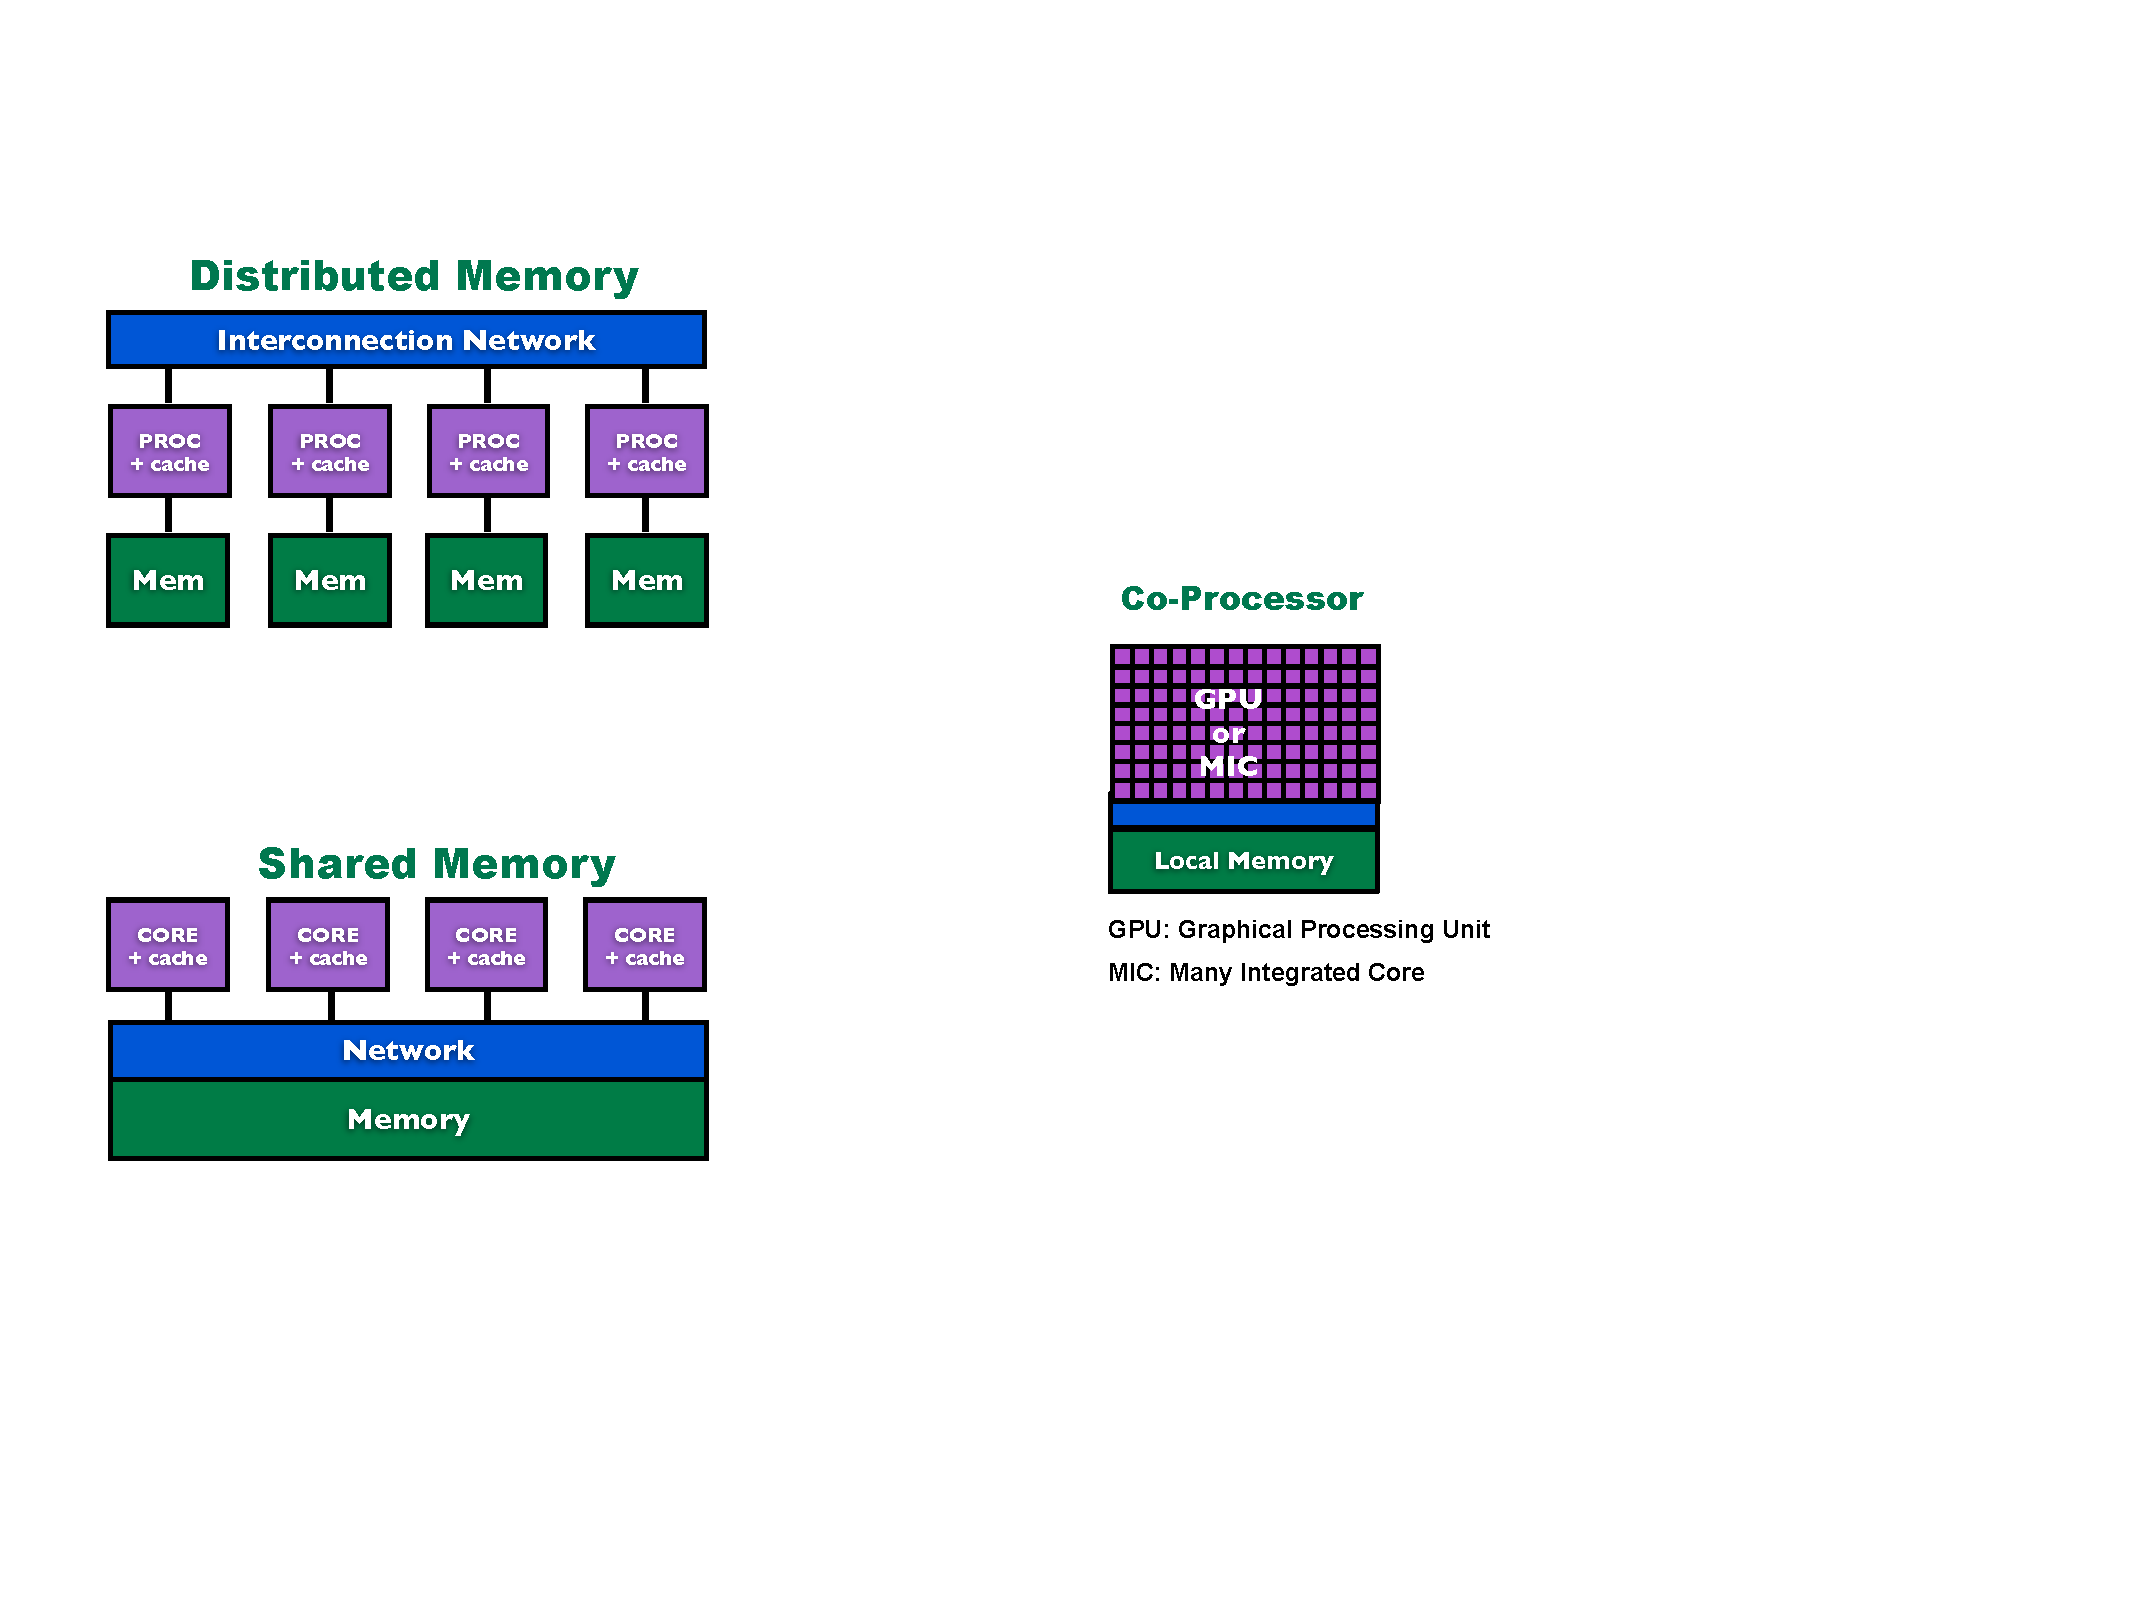
\includegraphics[width=0.95\textwidth]{../common/pics/ParallelHardware1.pdf}
\end{block}
\end{frame}

\begin{frame}
\begin{block}{Your Laptop or Desktop}
    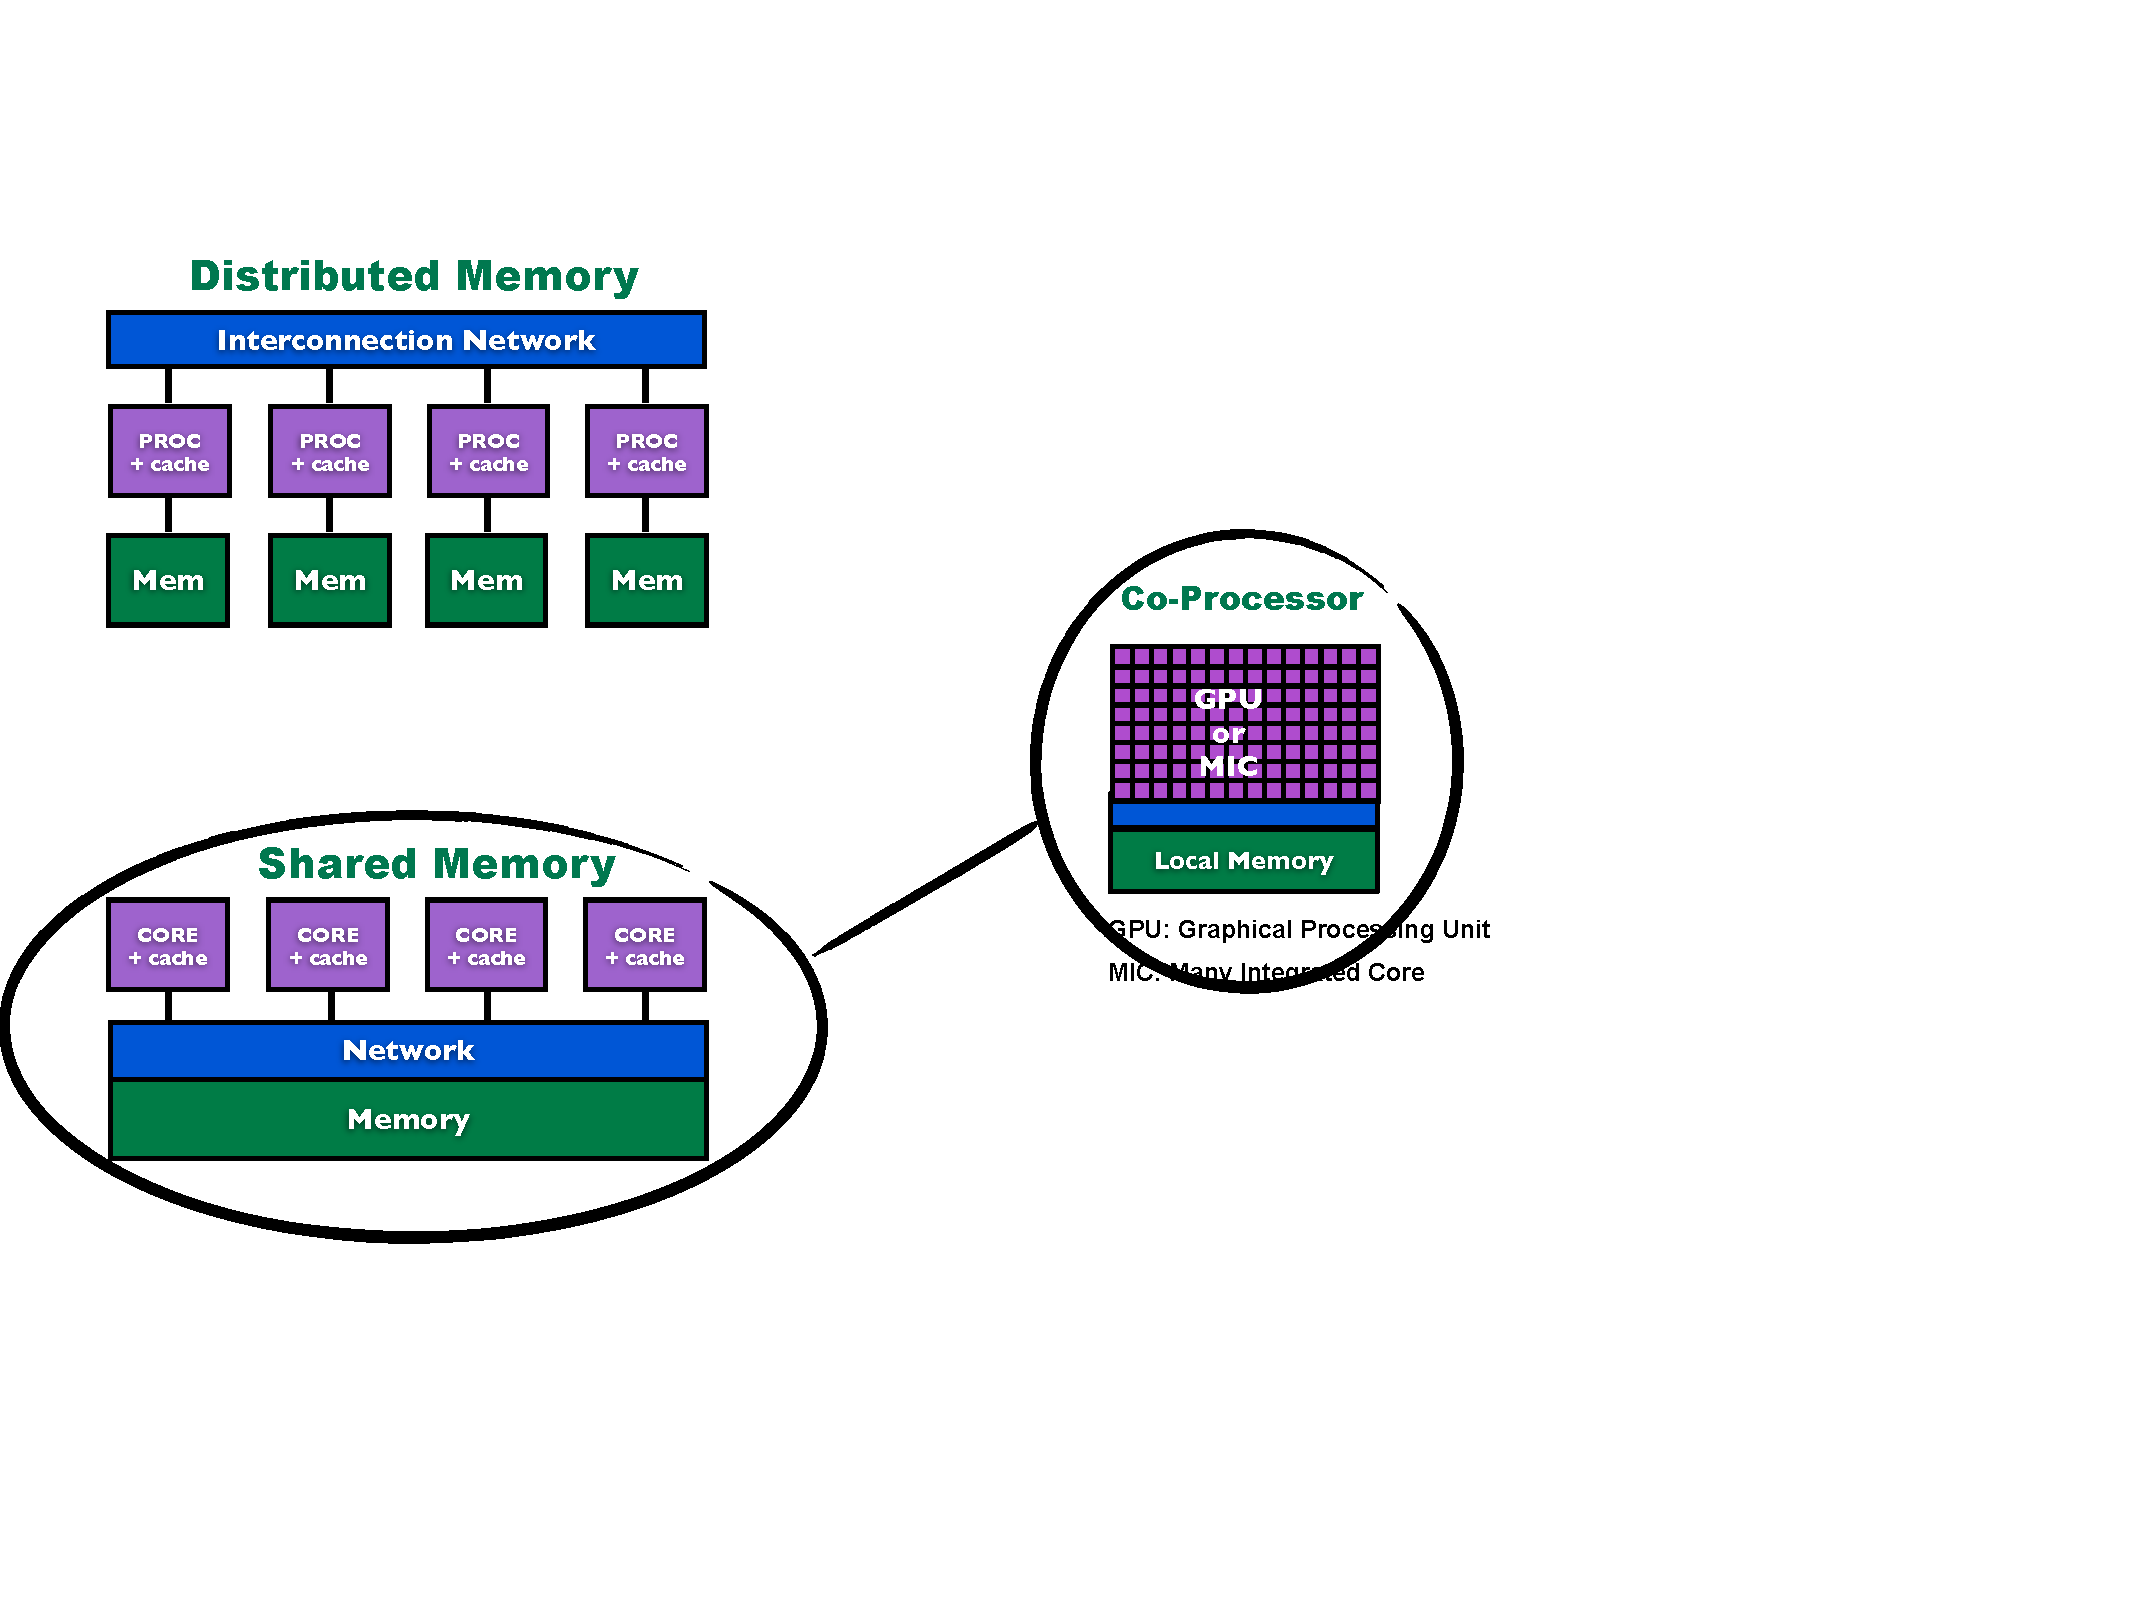
\includegraphics[width=0.95\textwidth]{../common/pics/ParallelHardware2.pdf}
\end{block}
\end{frame}

\begin{frame}
\begin{block}{A Server or Cluster}
    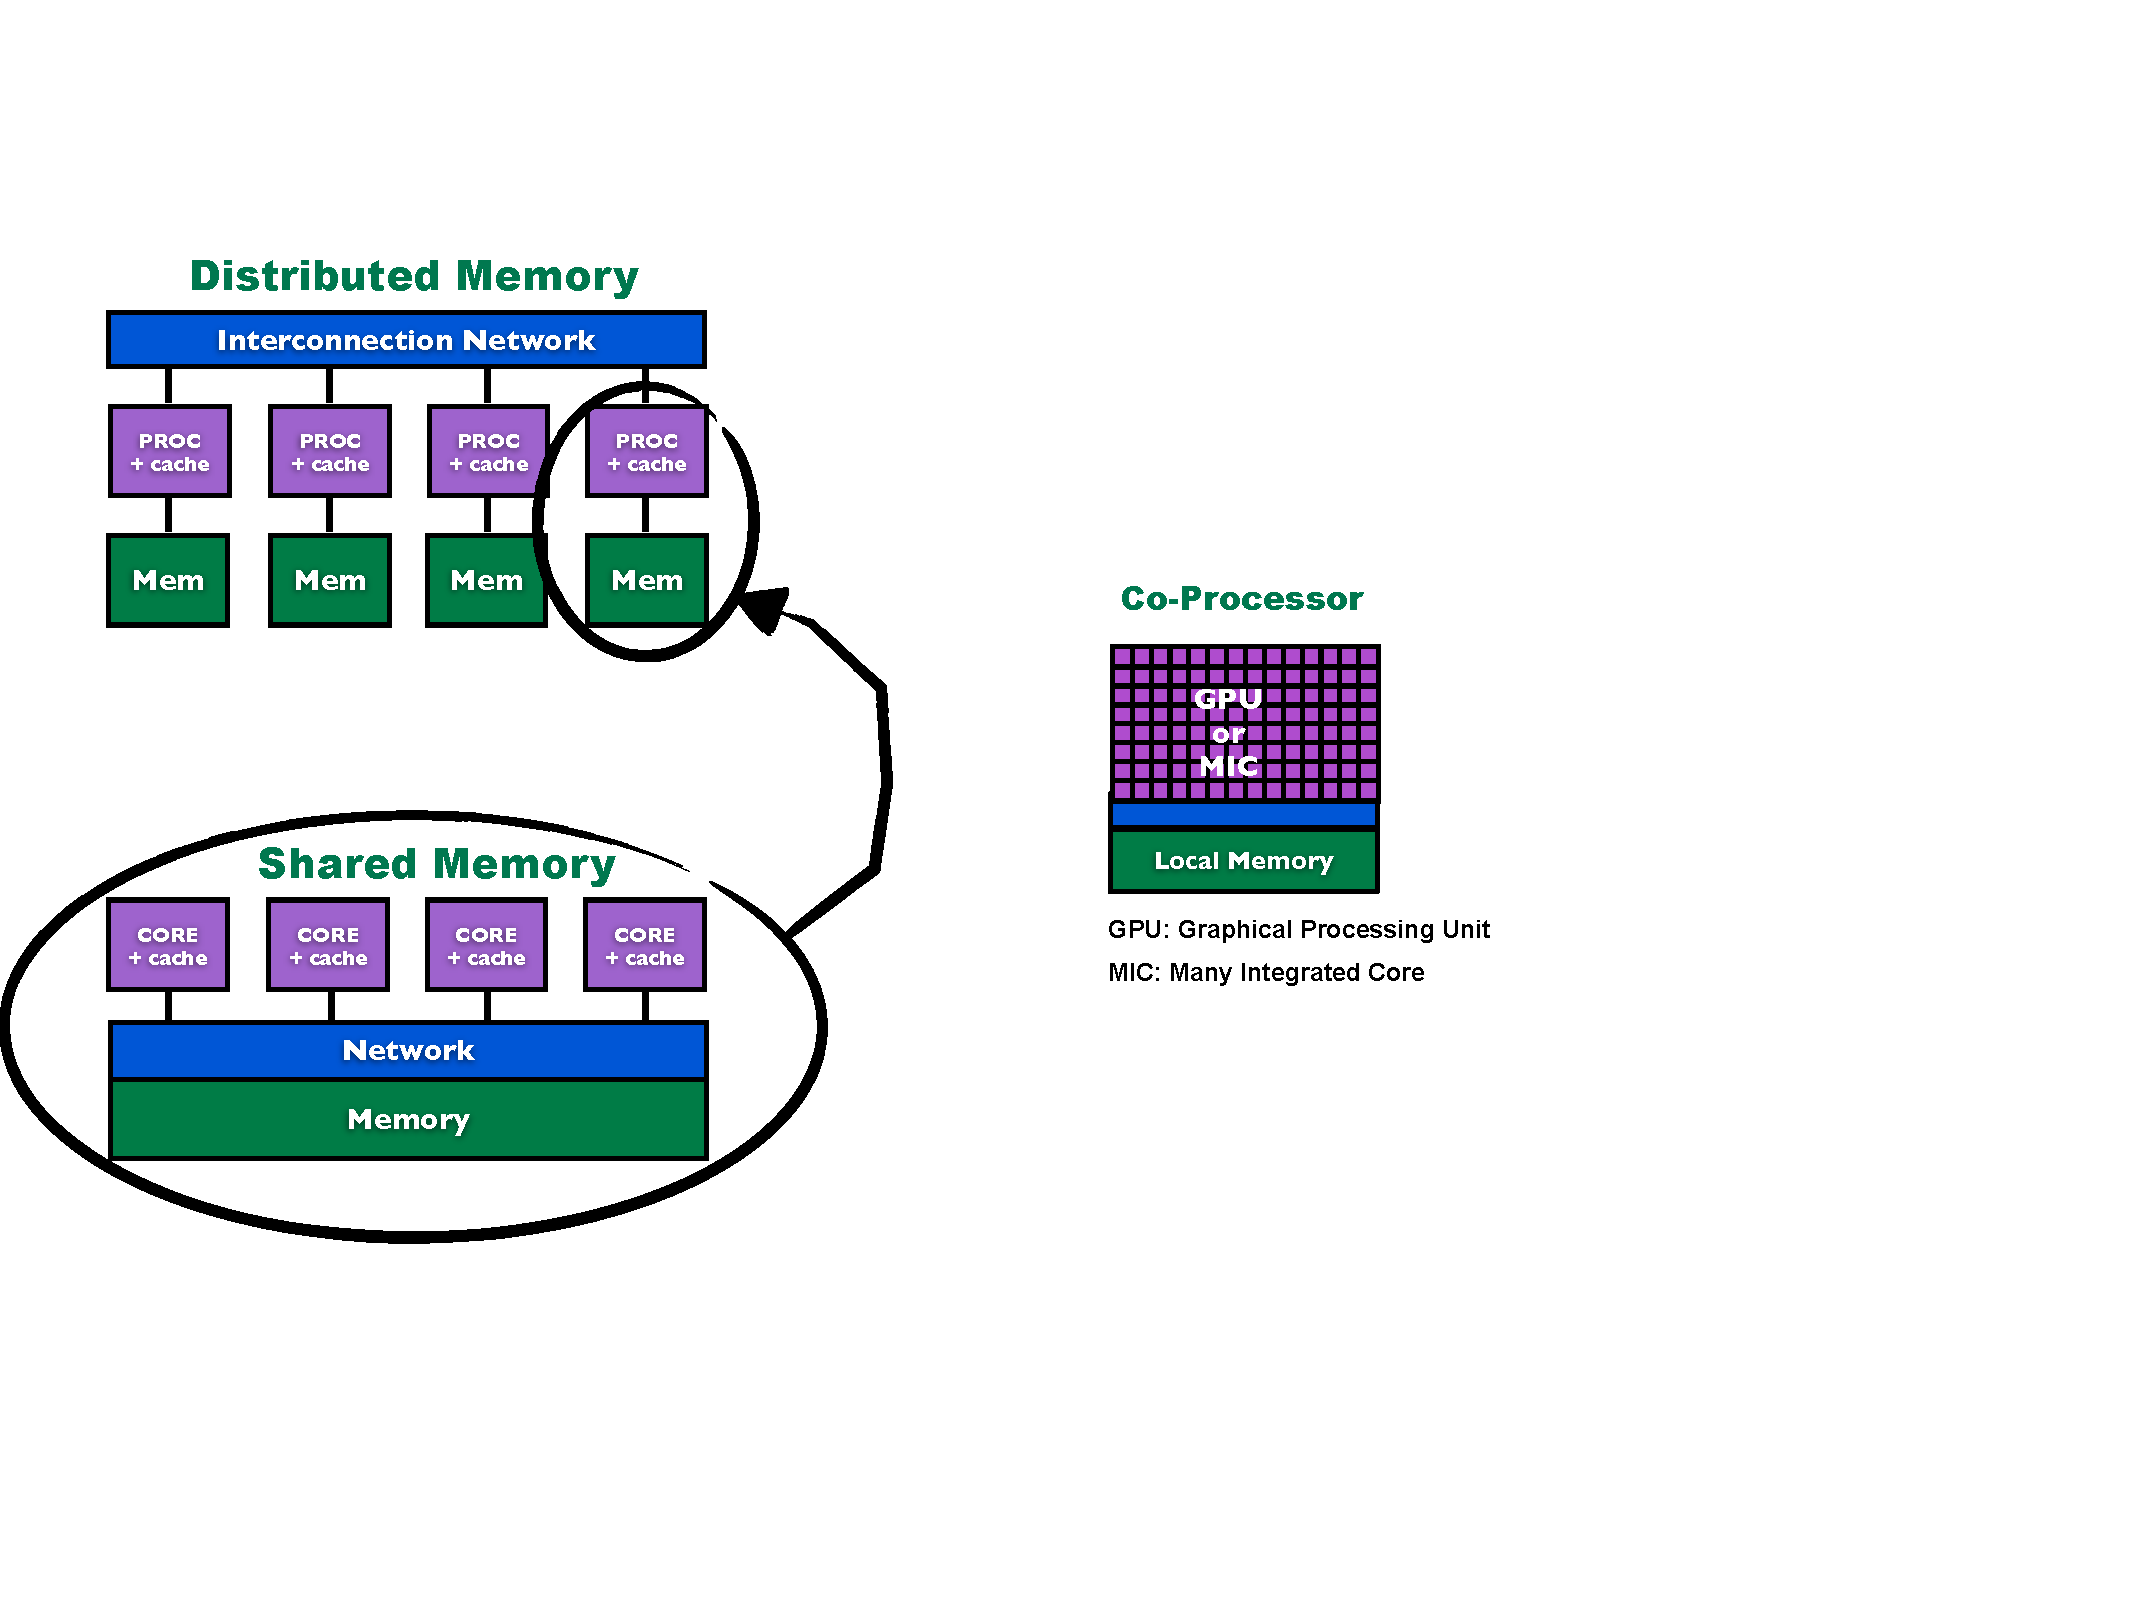
\includegraphics[width=0.95\textwidth]{../common/pics/ParallelHardware3.pdf}
\end{block}
\end{frame}

\begin{frame}
\begin{block}{Server to Supercomputer}
    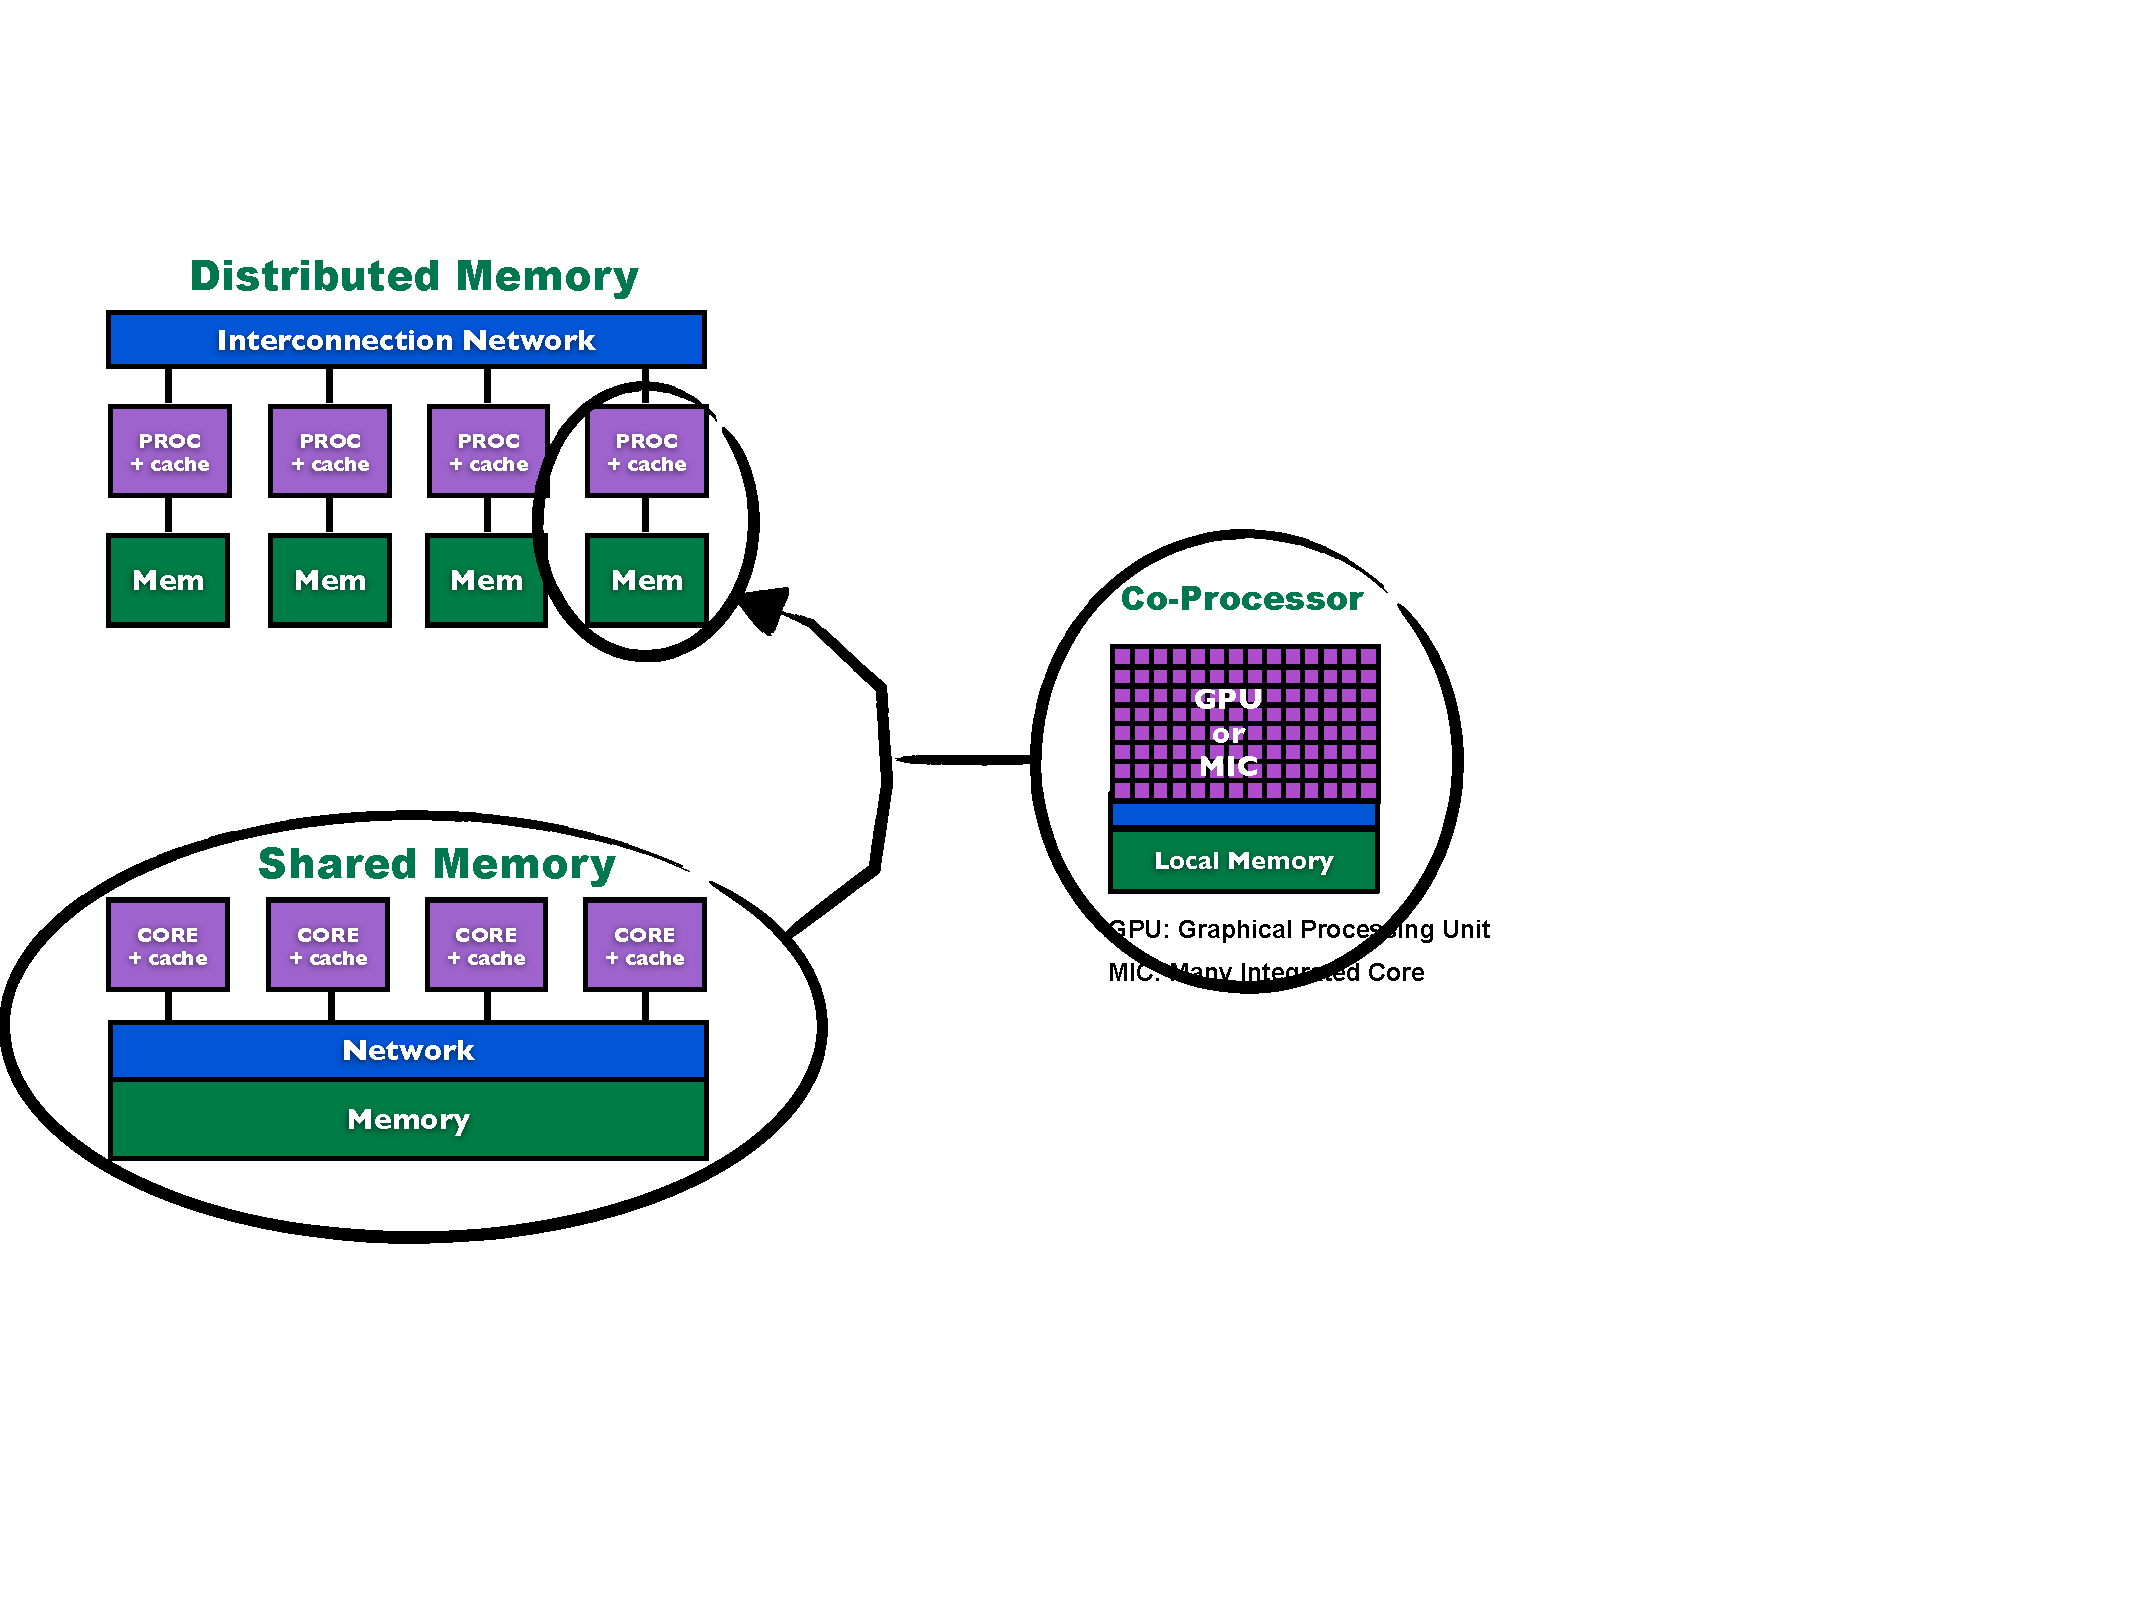
\includegraphics[width=0.95\textwidth]{../common/pics/ParallelHardware4.pdf}
\end{block}
\end{frame}

\begin{frame}
\begin{block}{Knowing the Right Words}
    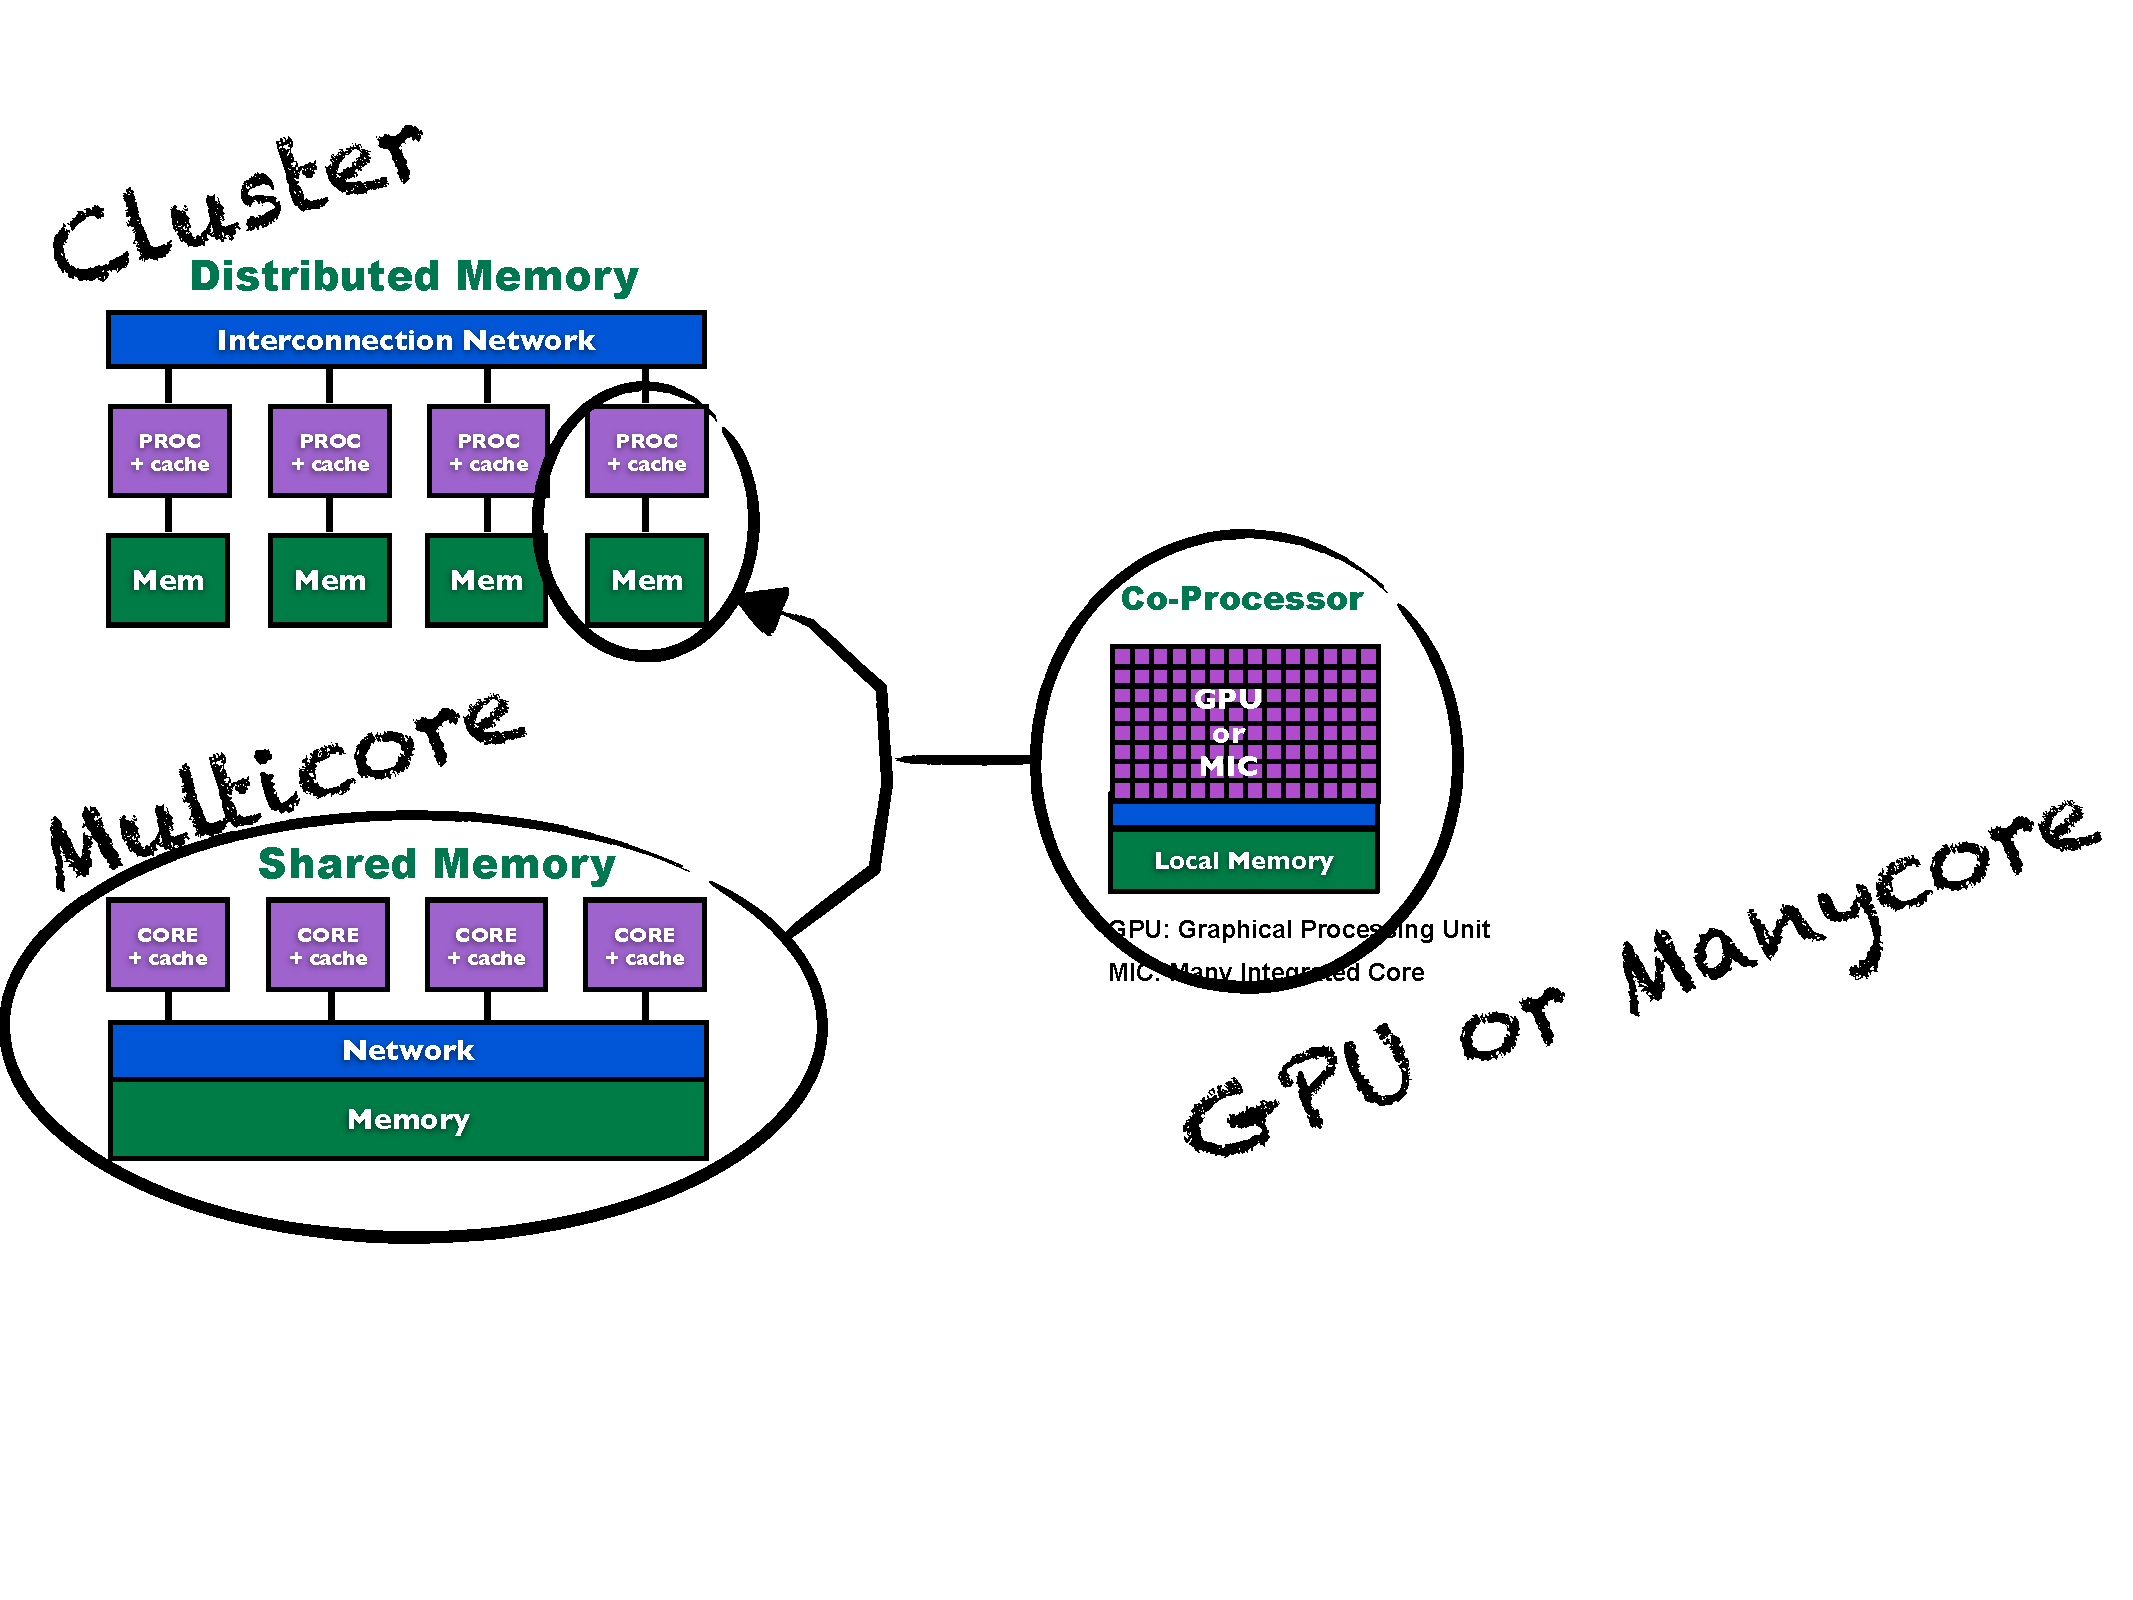
\includegraphics[width=0.95\textwidth]{../common/pics/ParallelHardware5.pdf}
\end{block}
\end{frame}

\begin{frame}
\begin{block}{``Native'' Programming Models and Tools}
    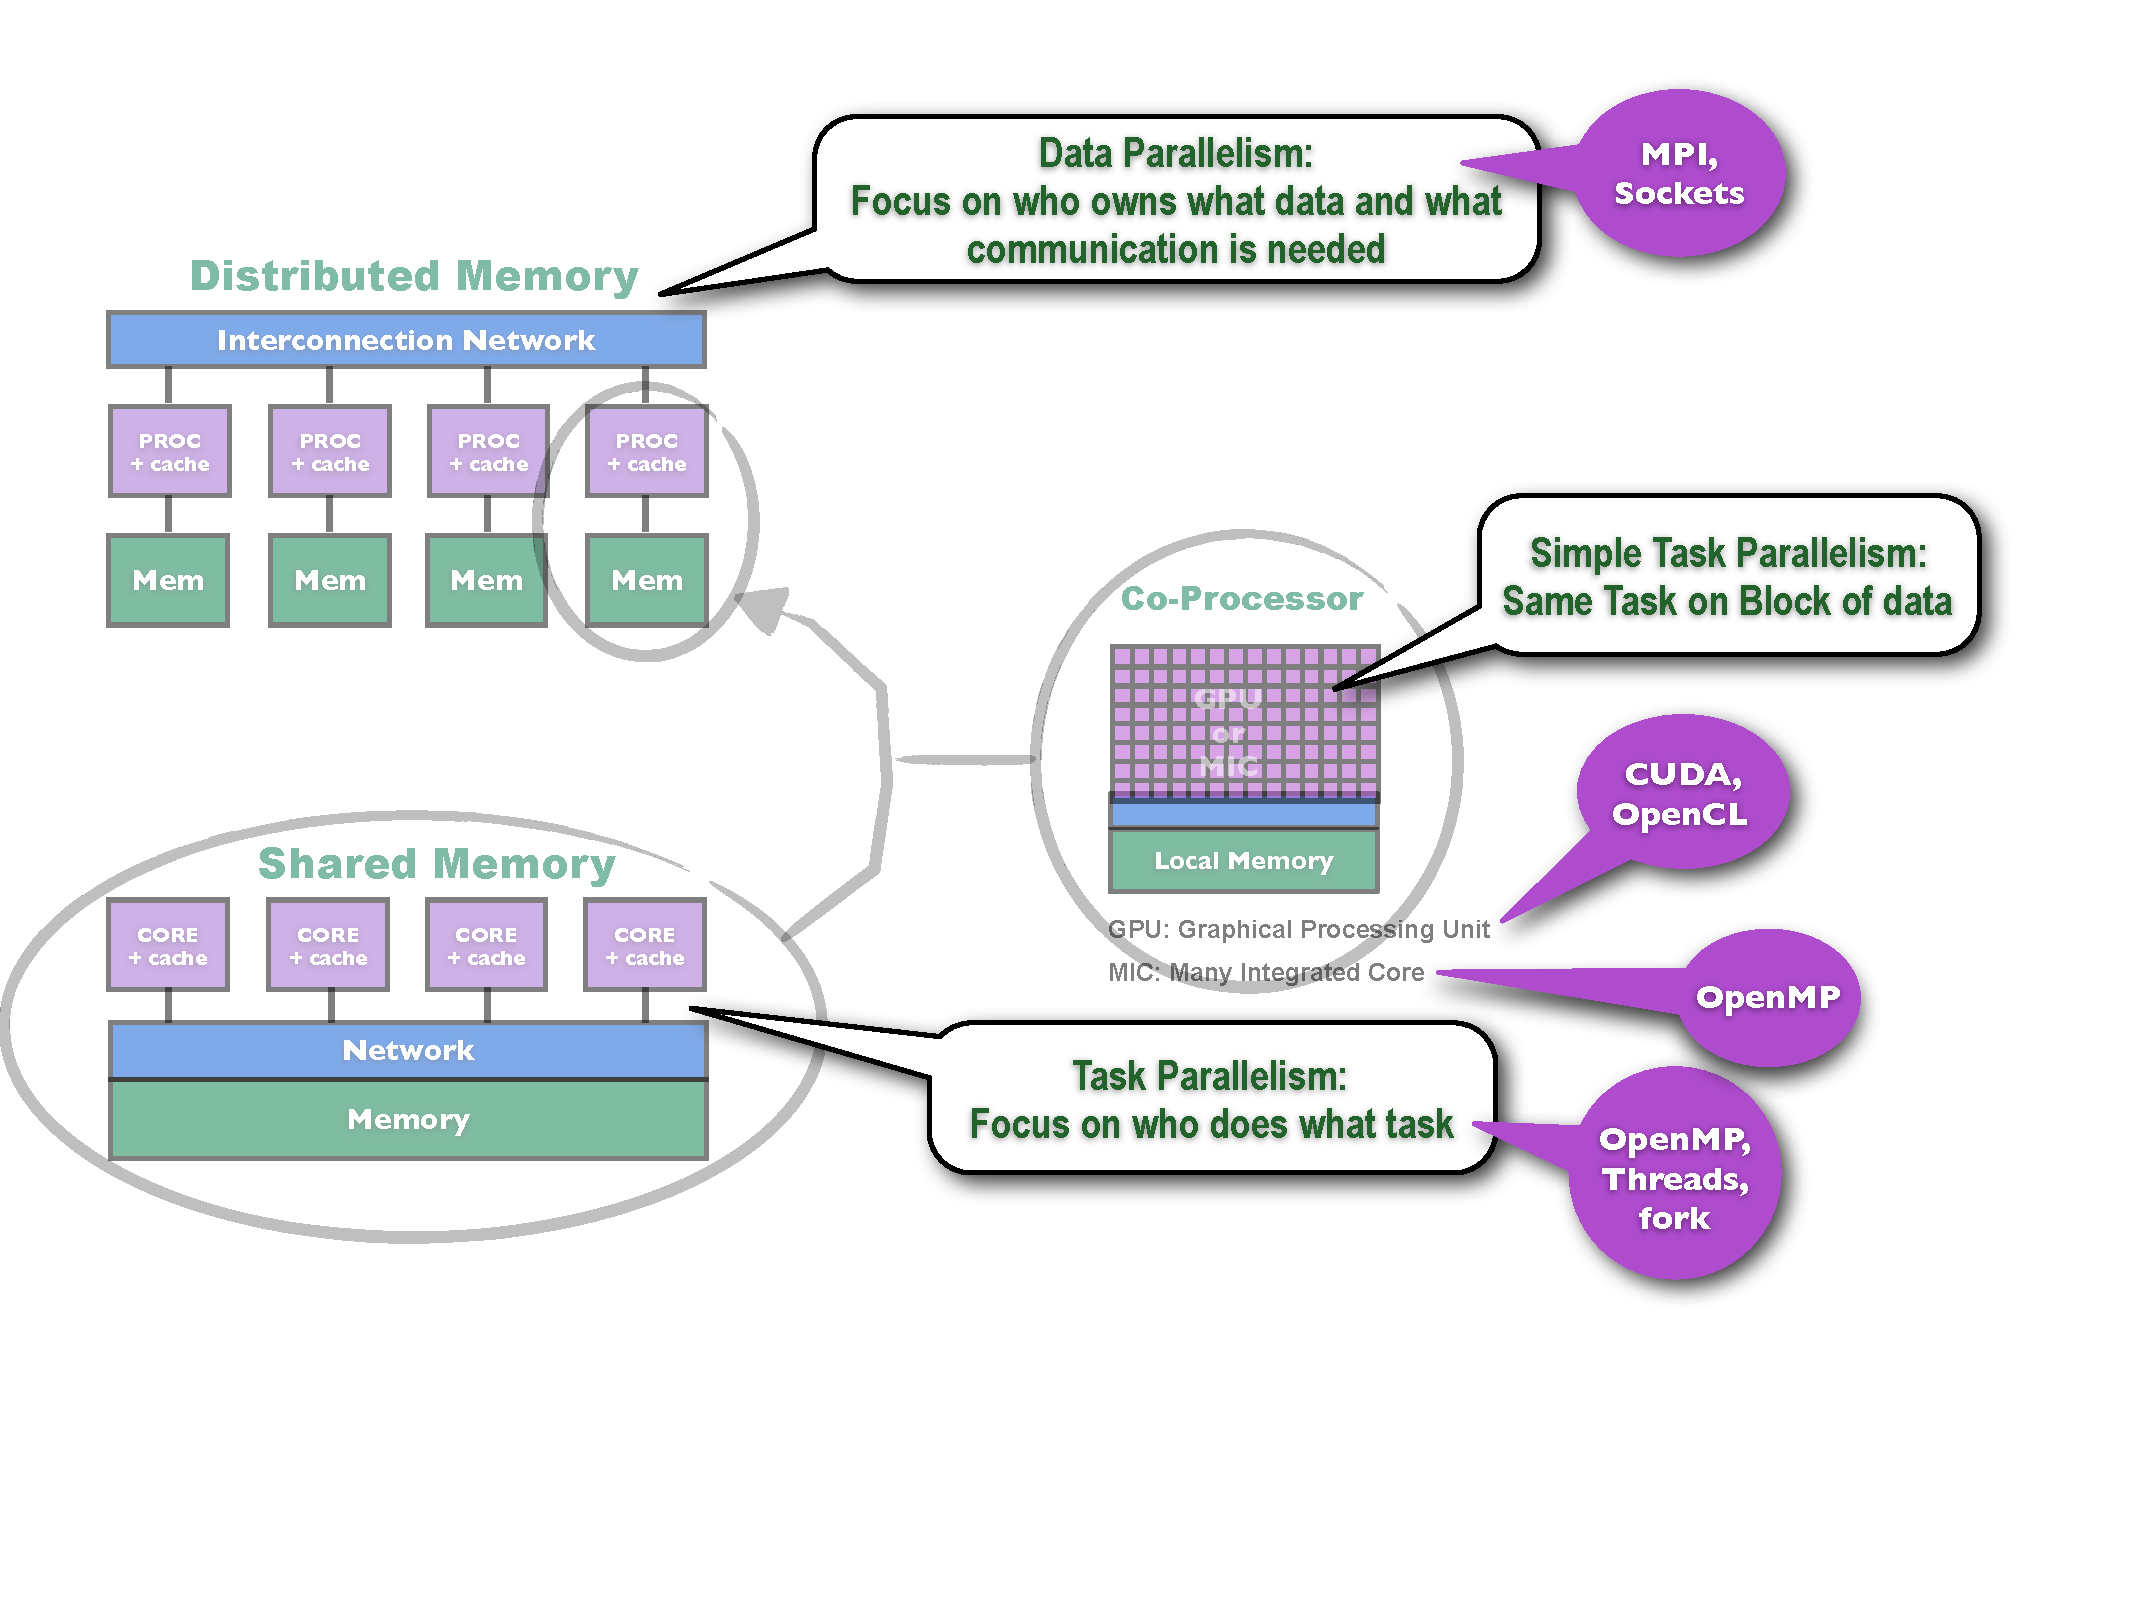
\includegraphics[width=0.95\textwidth]{../common/pics/ParallelHardware6.pdf}
\end{block}
\end{frame}

\begin{frame}
\begin{block}{R Interfaces to Native Tools}
    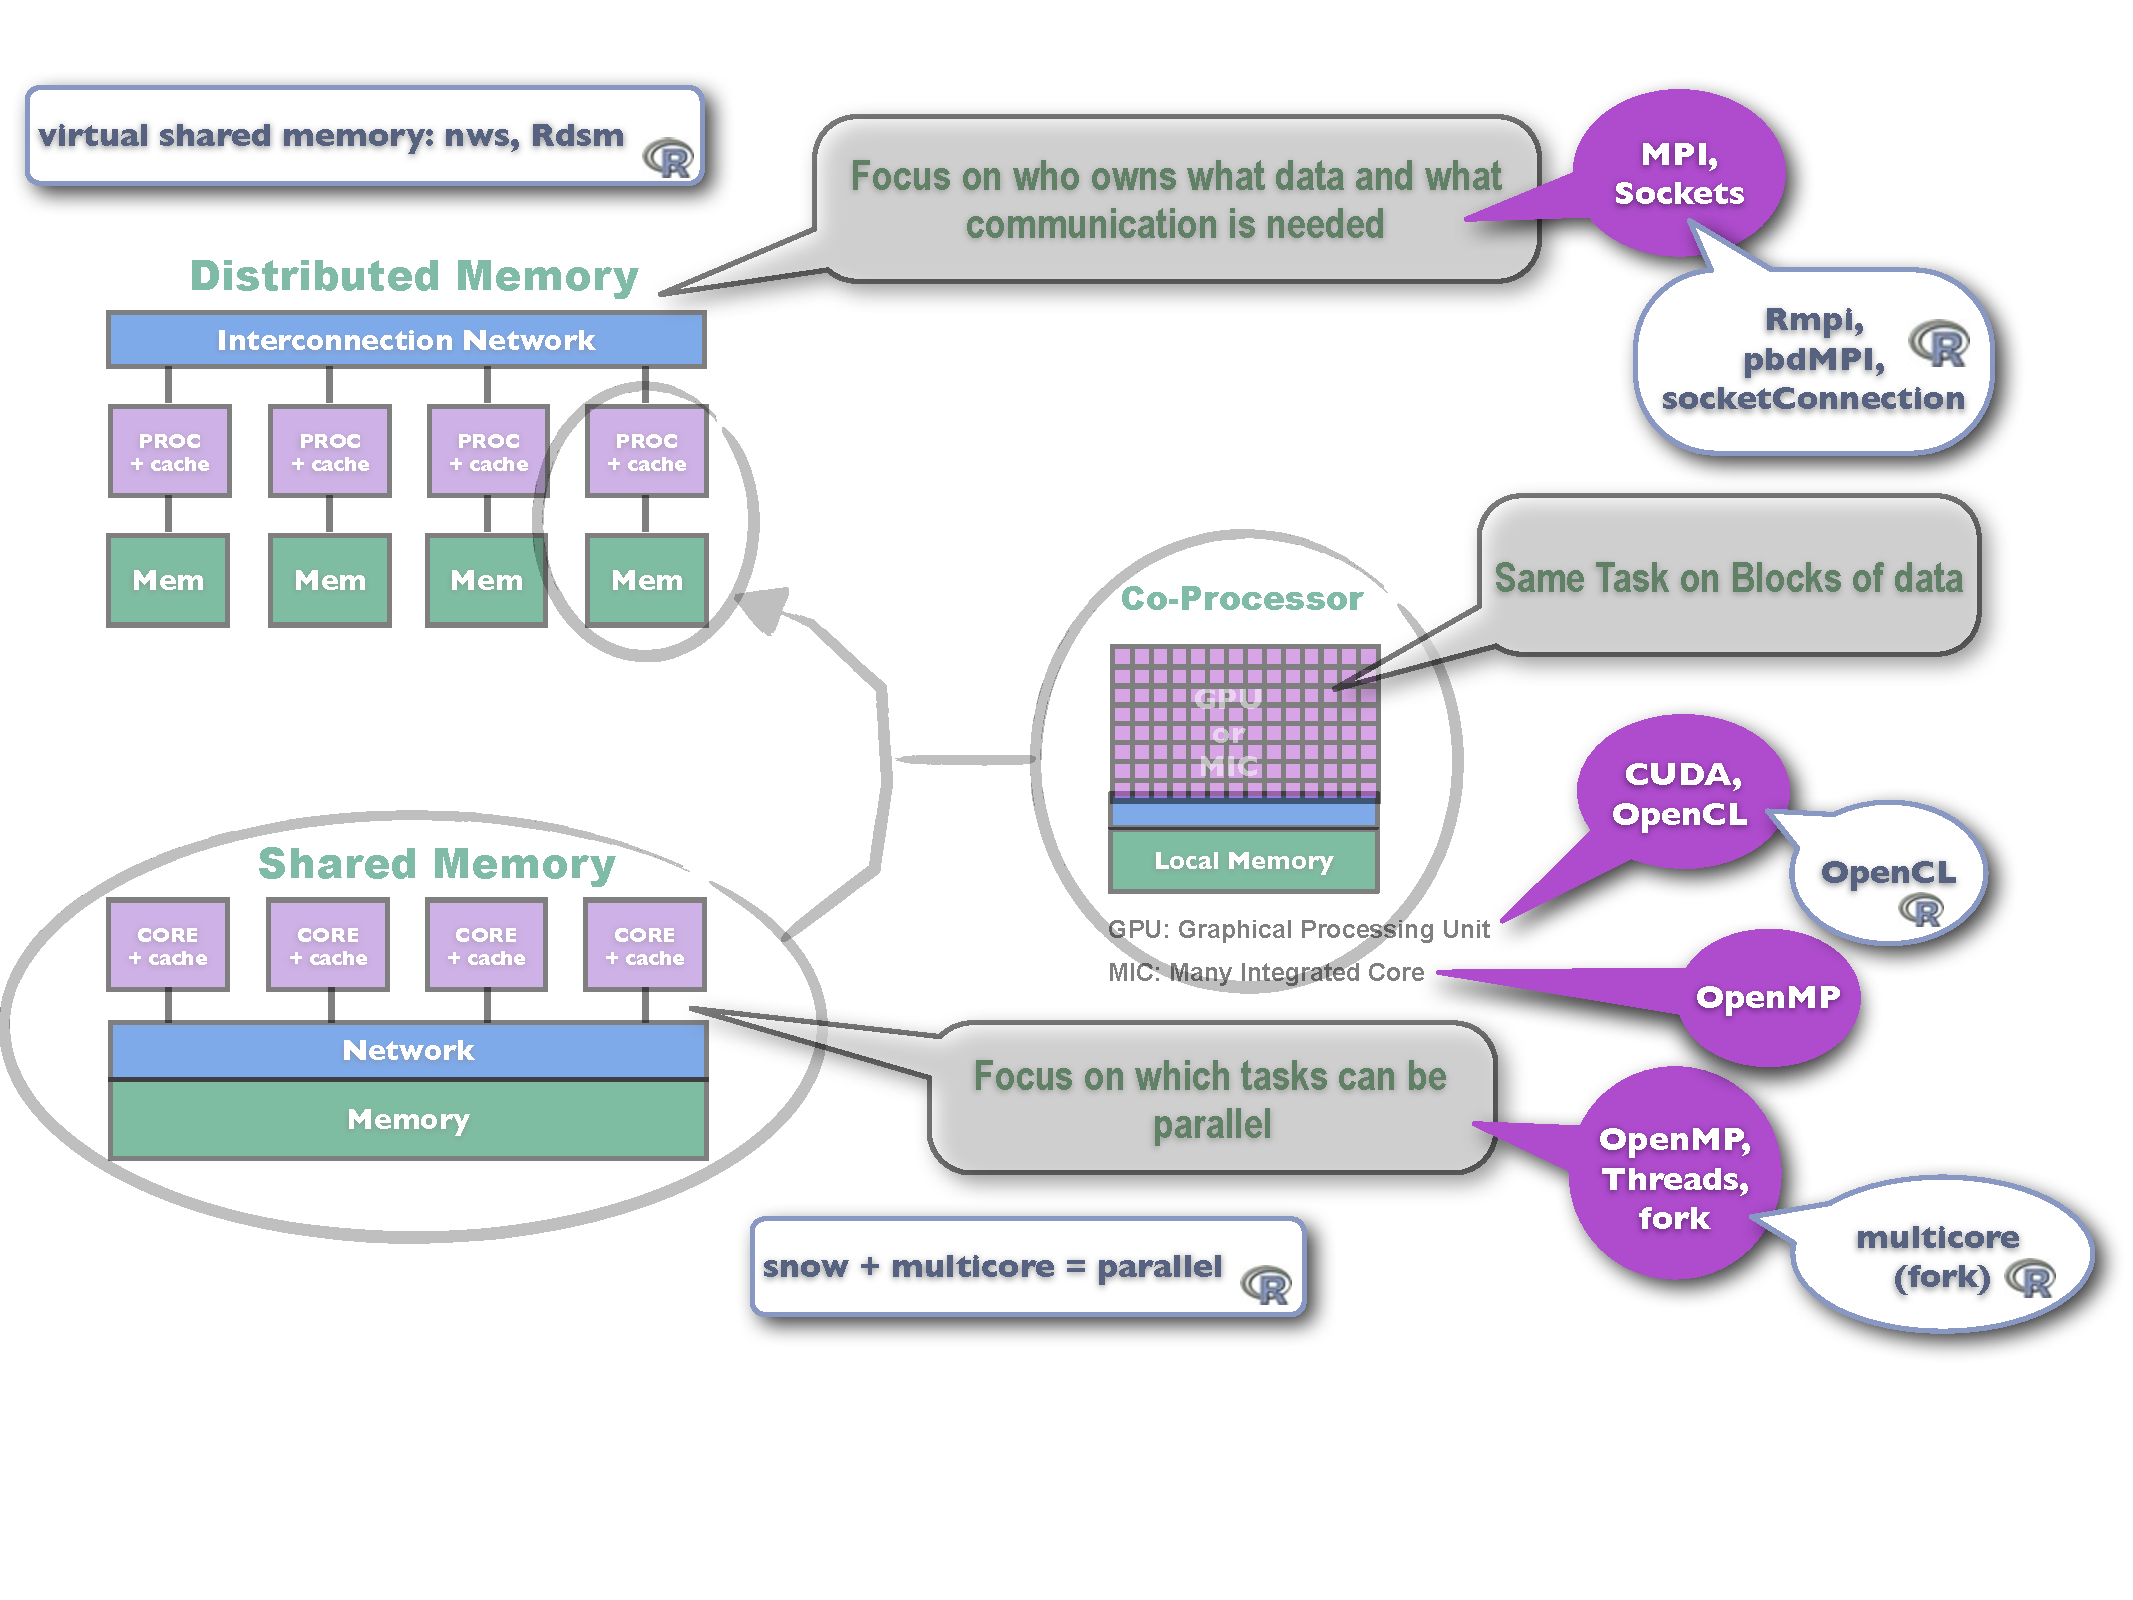
\includegraphics[width=0.95\textwidth]{../common/pics/ParallelHardware7.pdf}
\end{block}
\end{frame}

\begin{frame}
\begin{block}{30+ Years of Parallel Computing Research}
    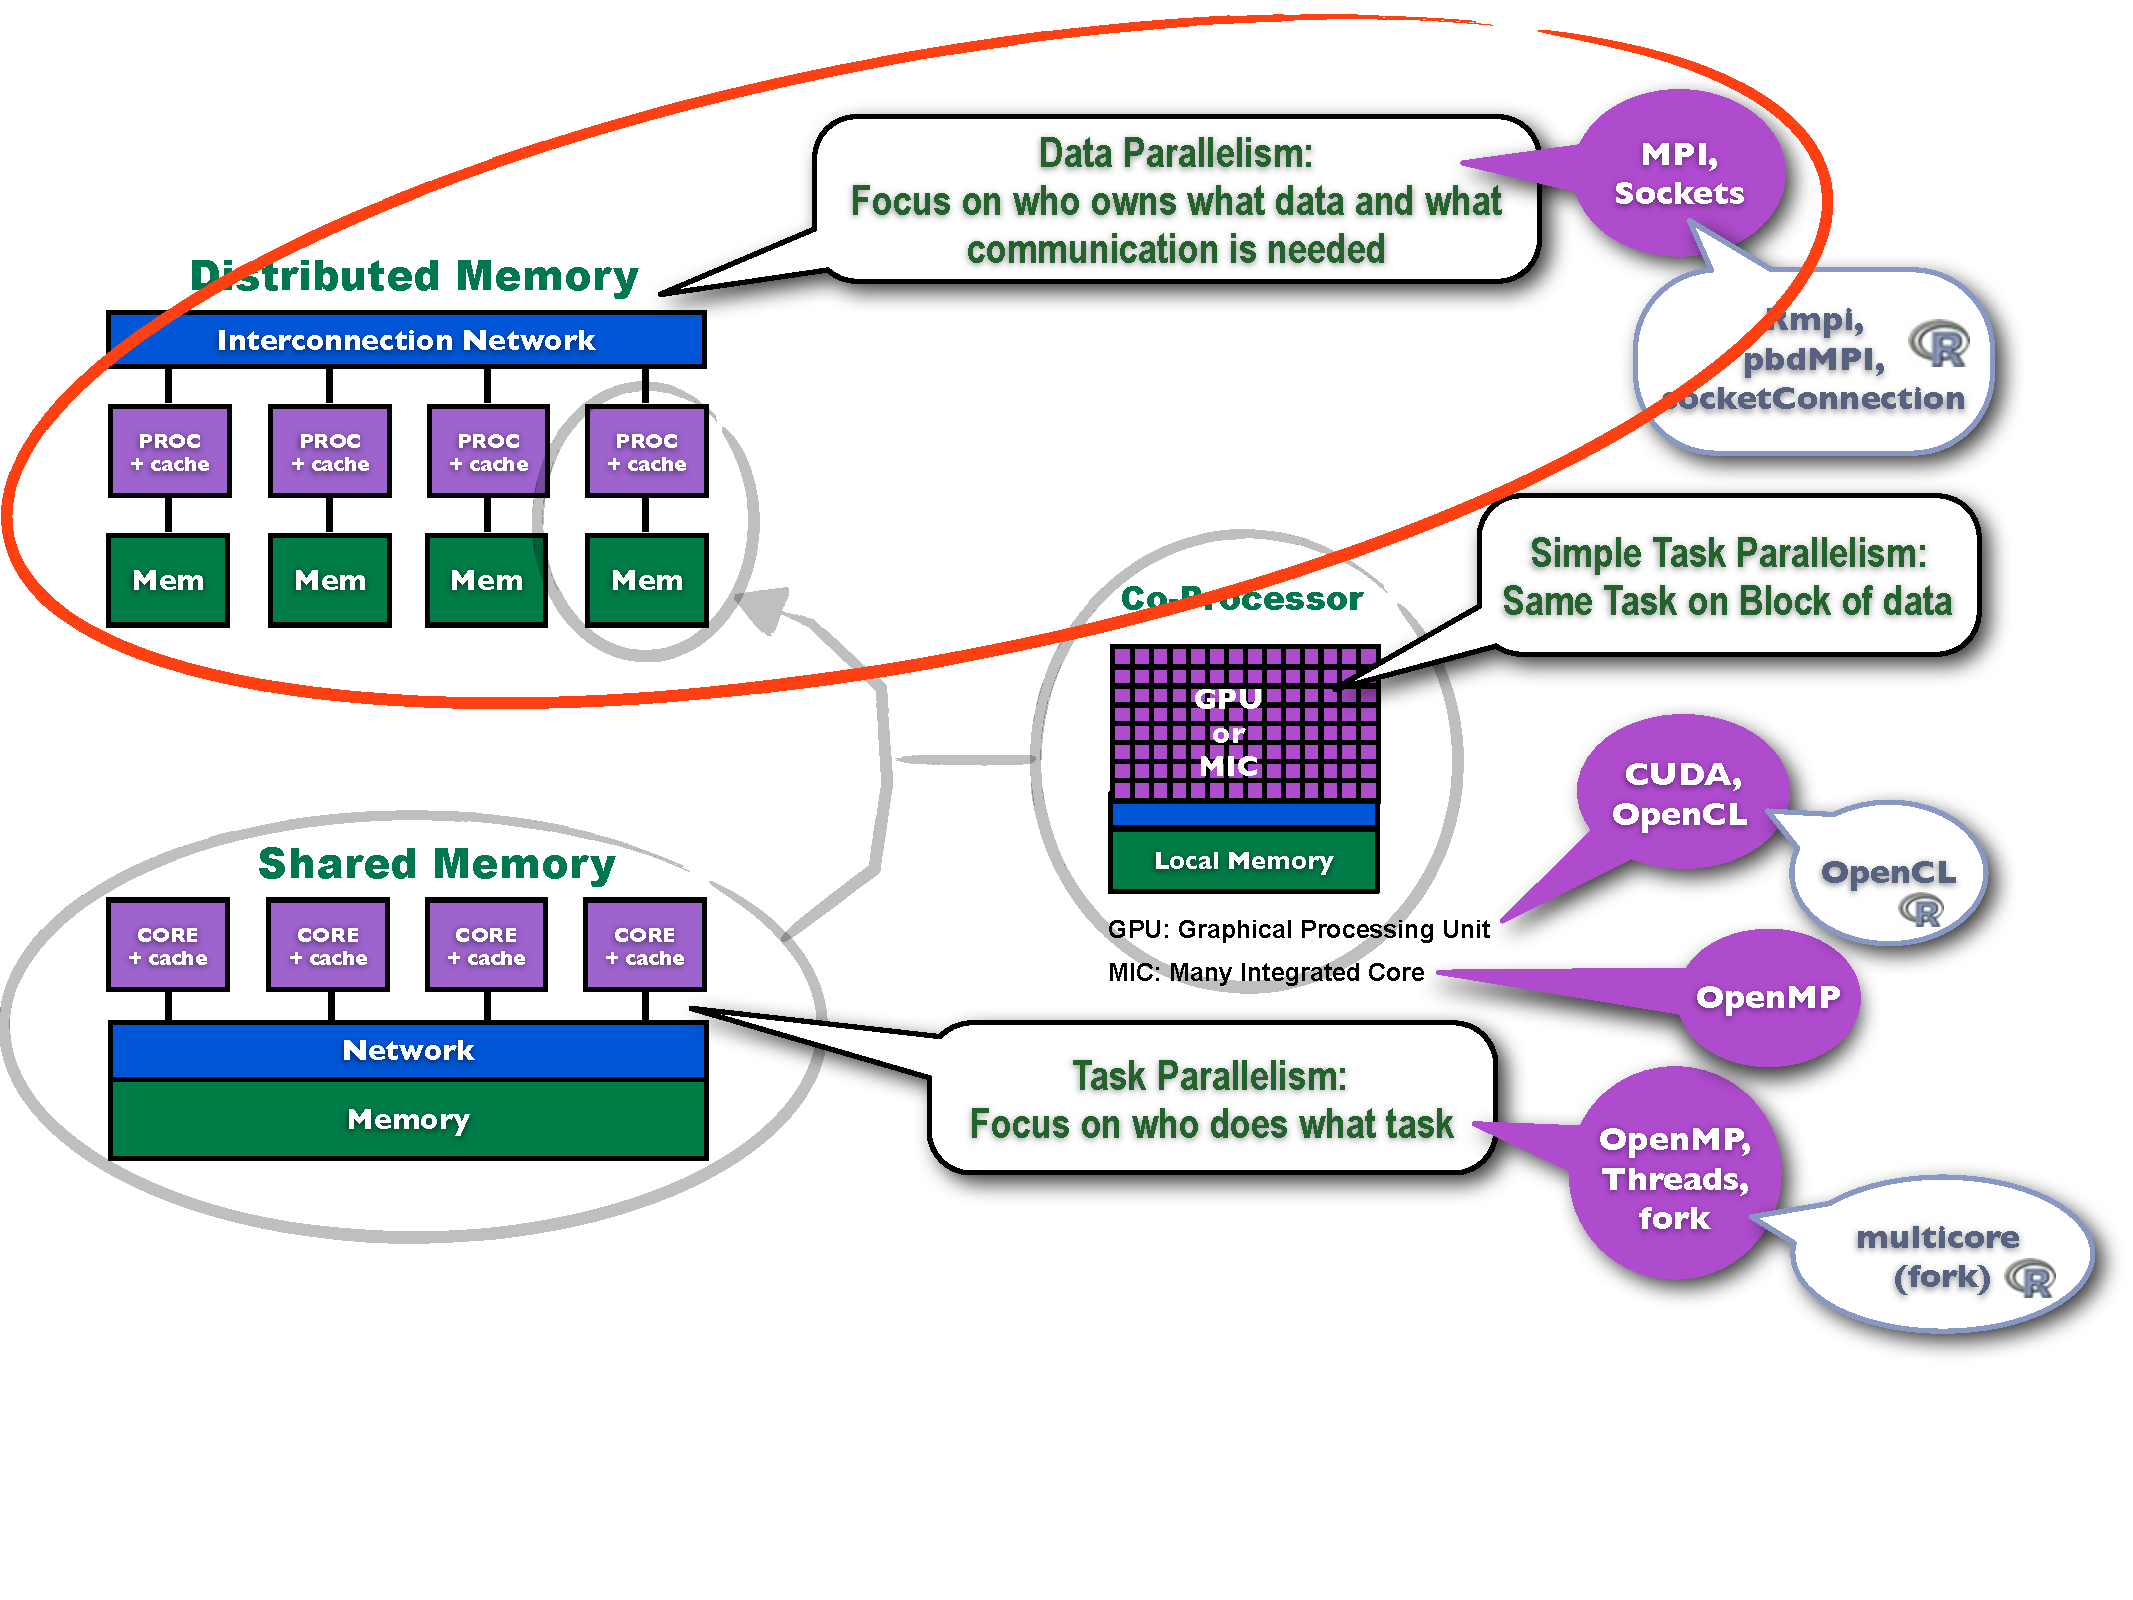
\includegraphics[width=0.95\textwidth]{../common/pics/ParallelHardware8.pdf}
\end{block}
\end{frame}

\begin{frame}
\begin{block}{Last 10 years of Advances}
    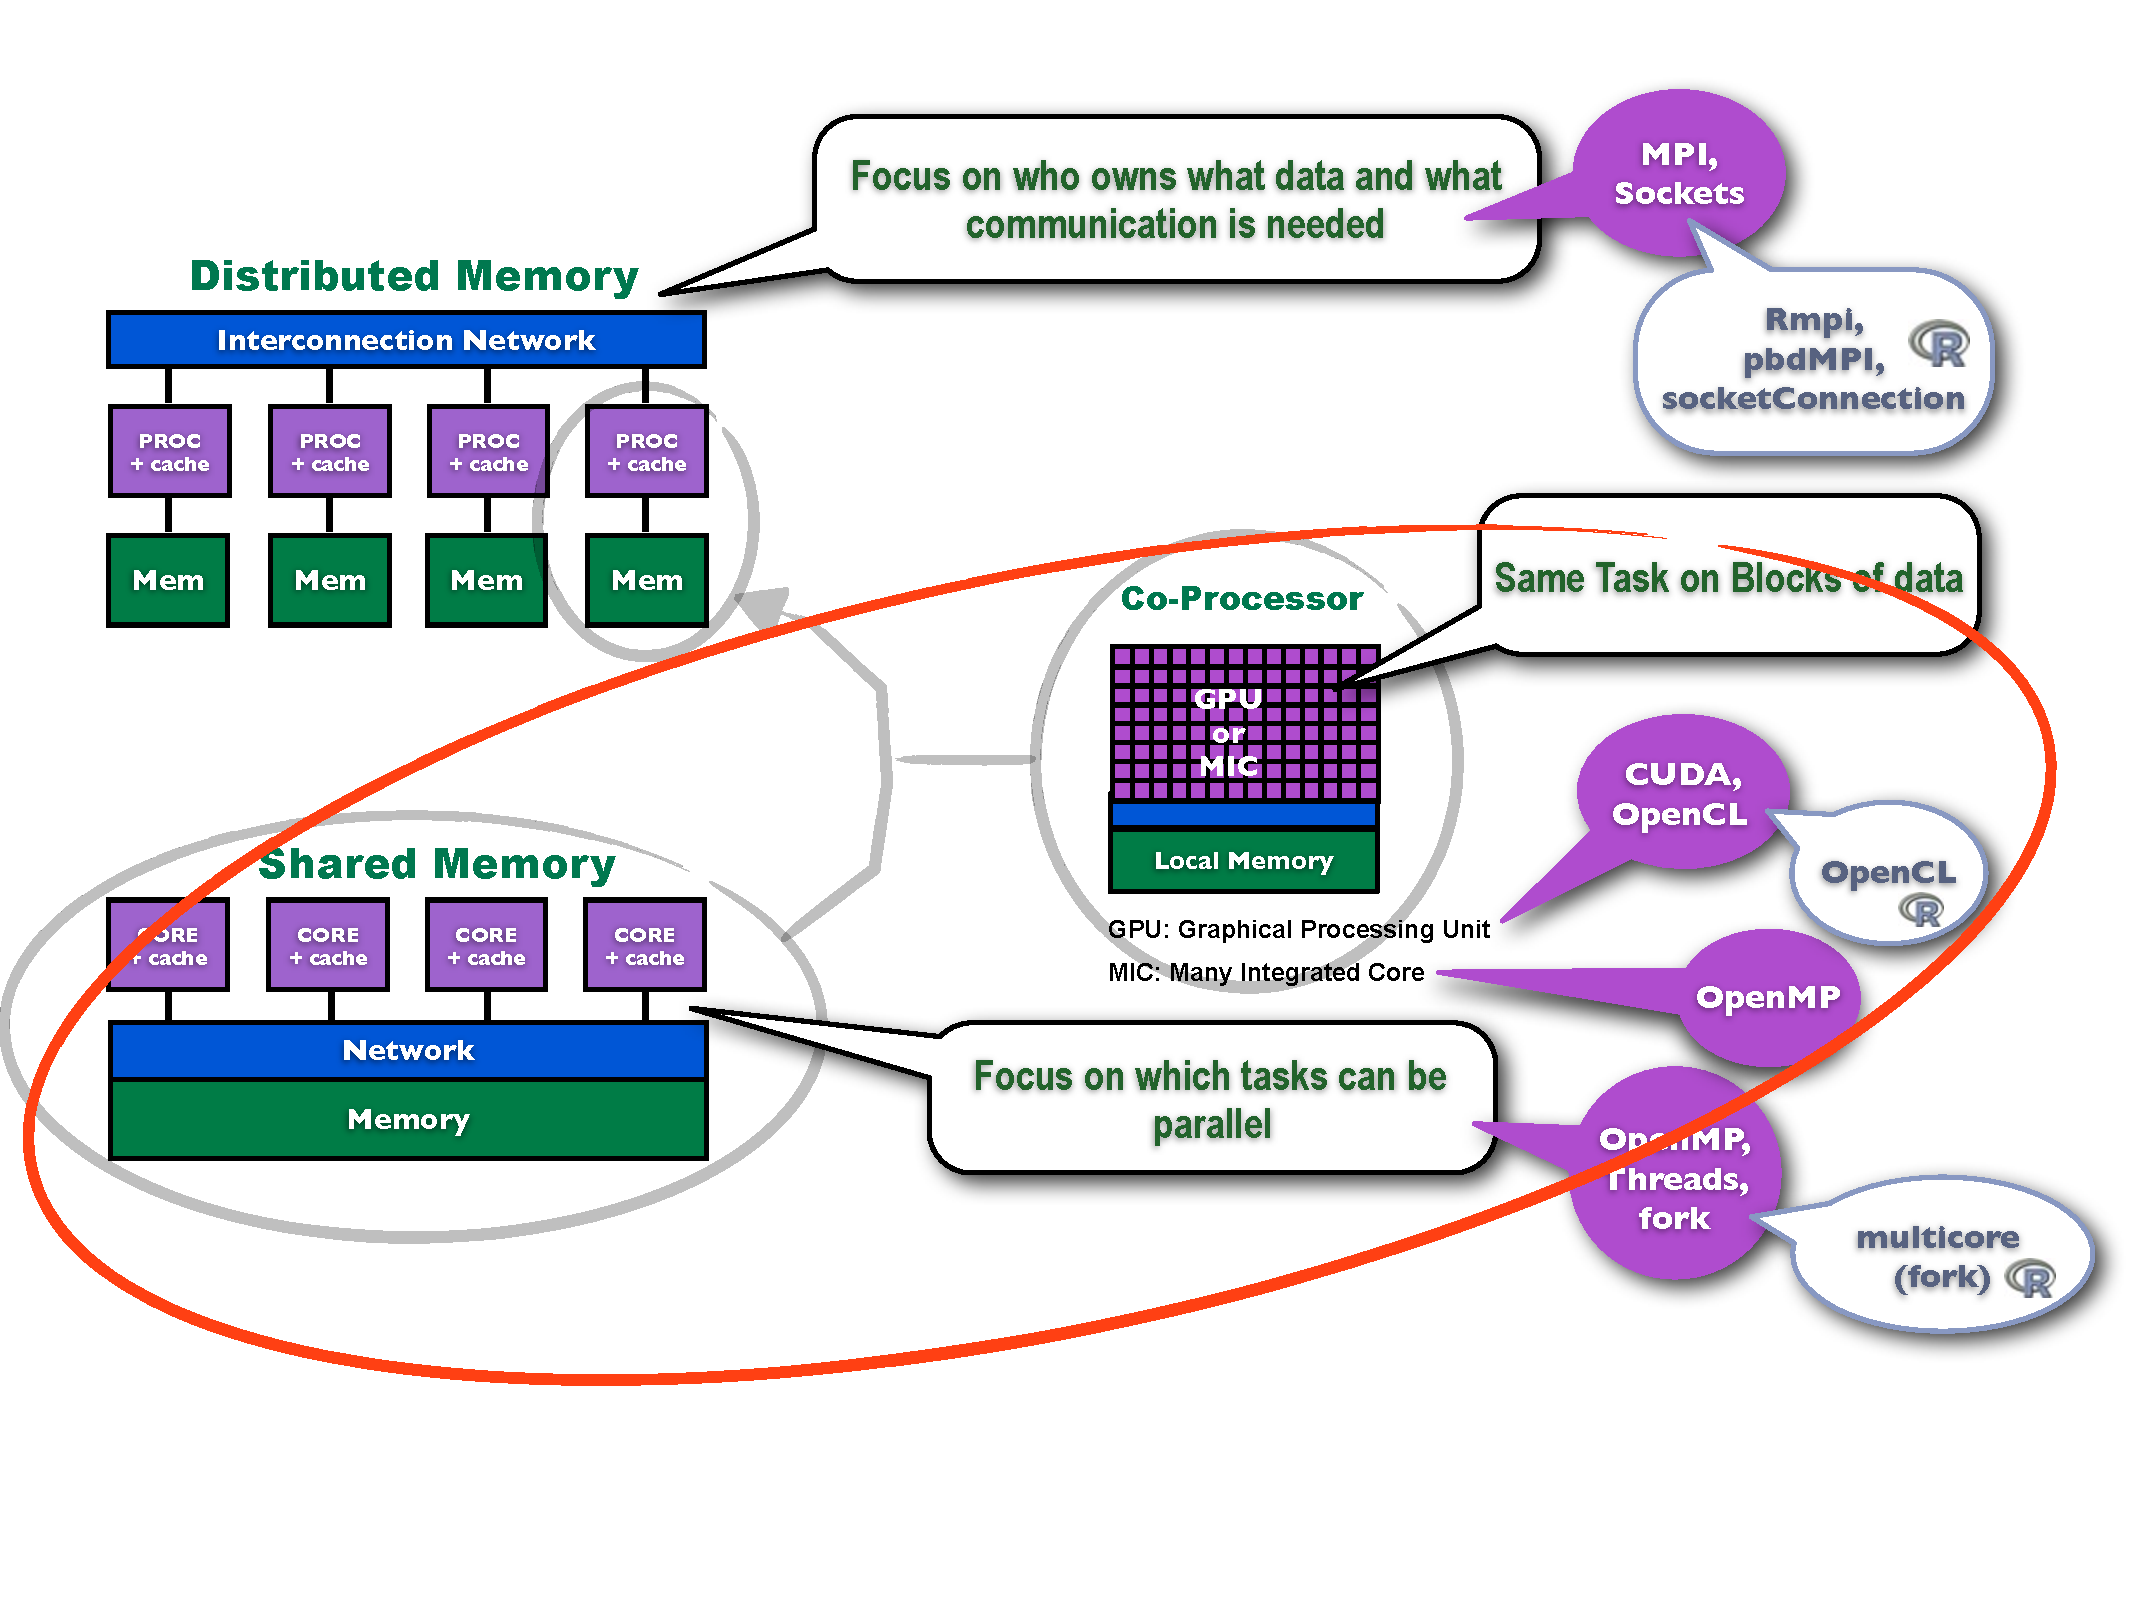
\includegraphics[width=0.95\textwidth]{../common/pics/ParallelHardware9.pdf}
\end{block}
\end{frame}

\begin{frame}
\begin{block}{Putting It All Together Challenge}
    
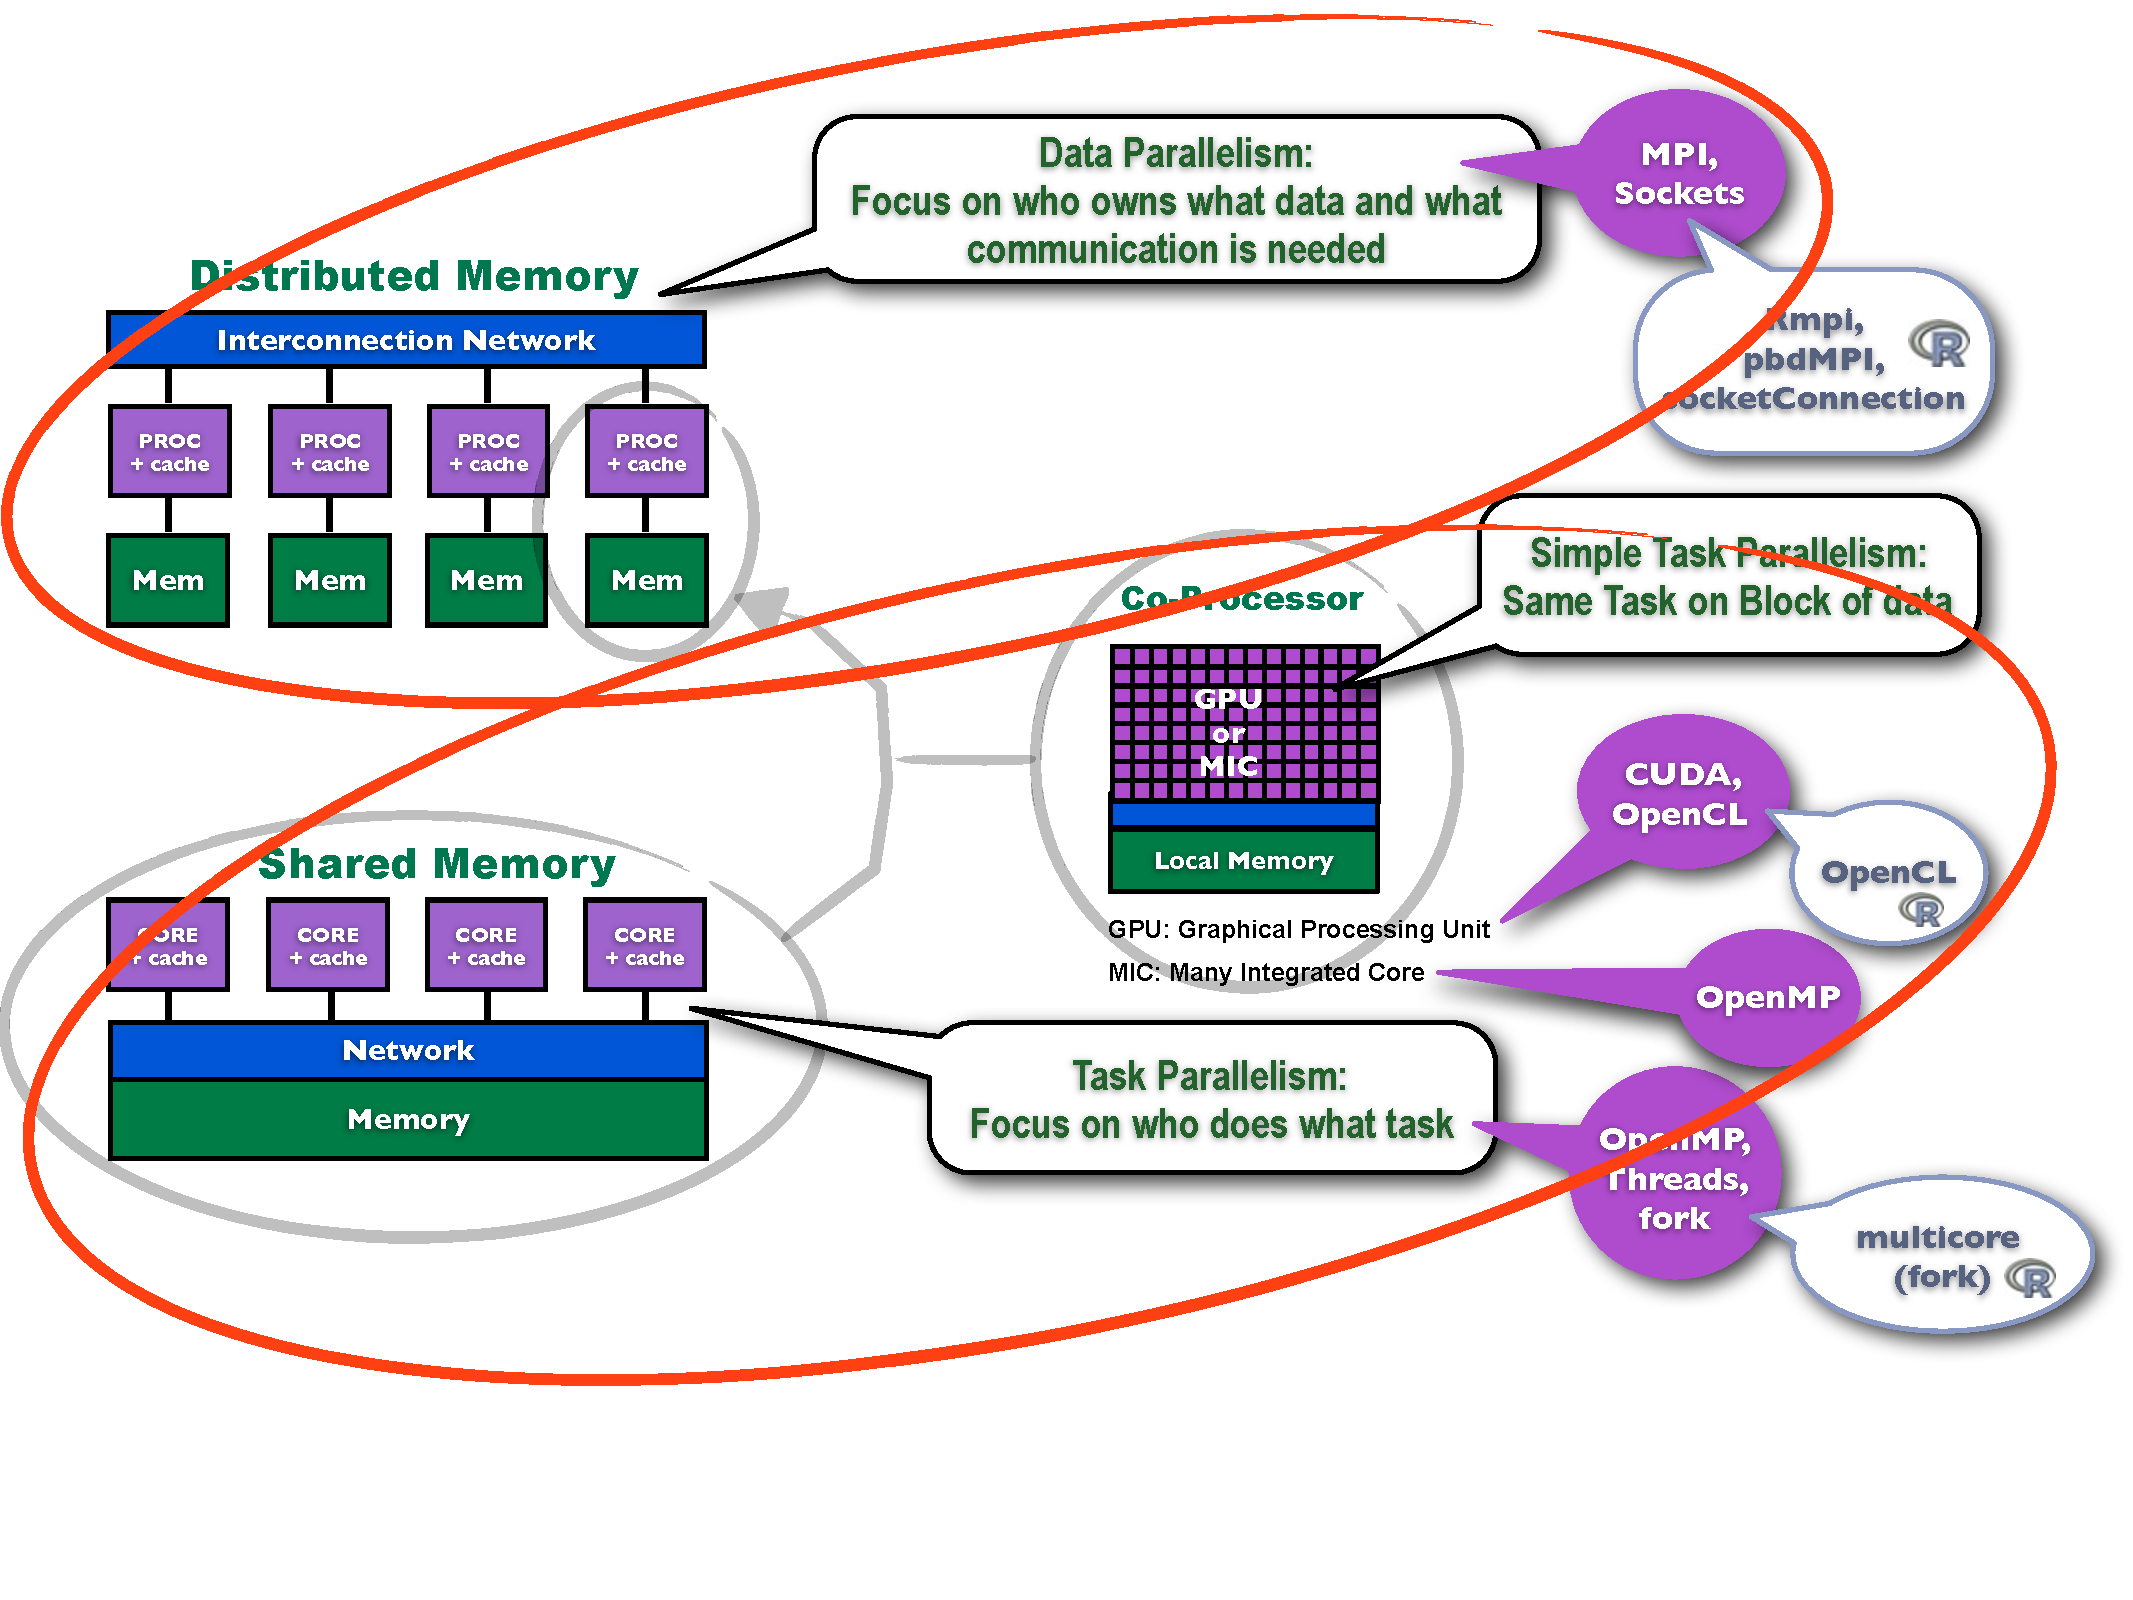
\includegraphics[width=0.95\textwidth]{../common/pics/ParallelHardware10.pdf}
\end{block}
\end{frame}

\begin{frame}
\begin{block}{pbdR Focus on Data Parallelism}
    
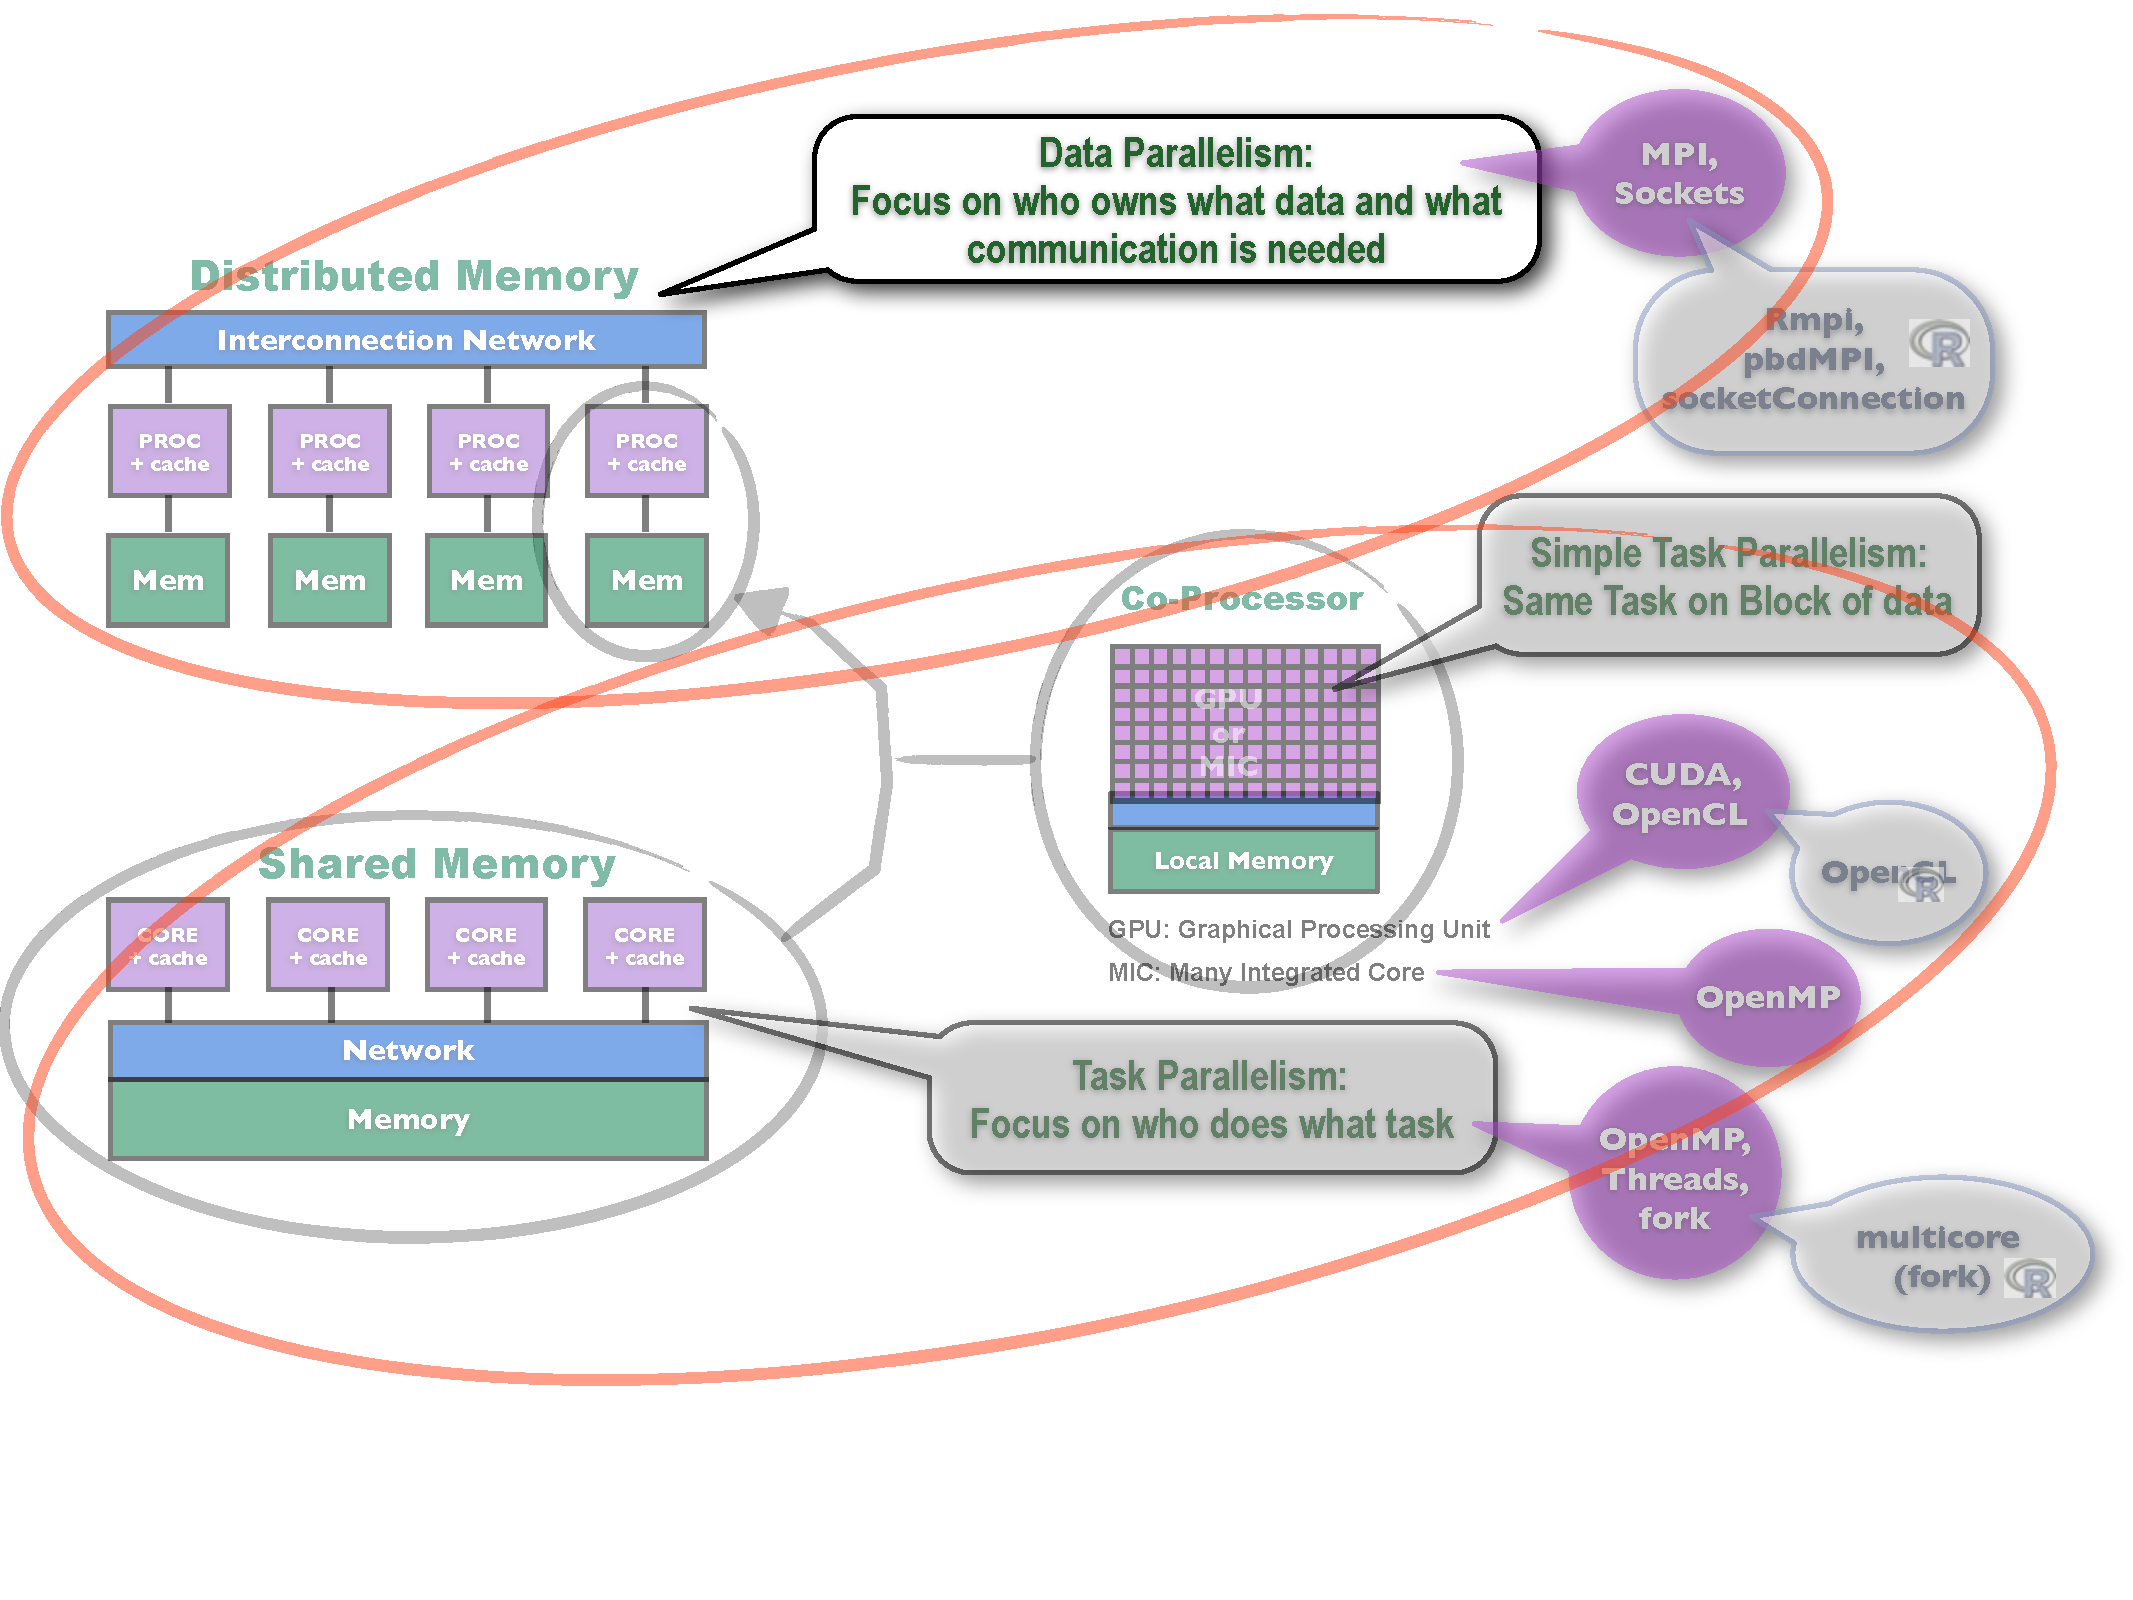
\includegraphics[width=0.95\textwidth]{../common/pics/ParallelHardware11.pdf}
\end{block}
\end{frame}


%%% Intro to parallelism
% \subsection{A Concise Introduction to Parallelism}

\begin{frame}
  \begin{block}{What is Parallelism?}\pause
  \begin{itemize}
    \item Doing more than one thing at a time.
    \item The simultaneous use of multiple compute resources to solve a 
computational problem.
  \end{itemize}
  \end{block}
\end{frame}

\begin{frame}
  \begin{block}{Parallelism}\pause
    \begin{center}
    \begin{minipage}{.46\textwidth}
    \begin{block}{\centering Serial Programming}
      \begin{center}
      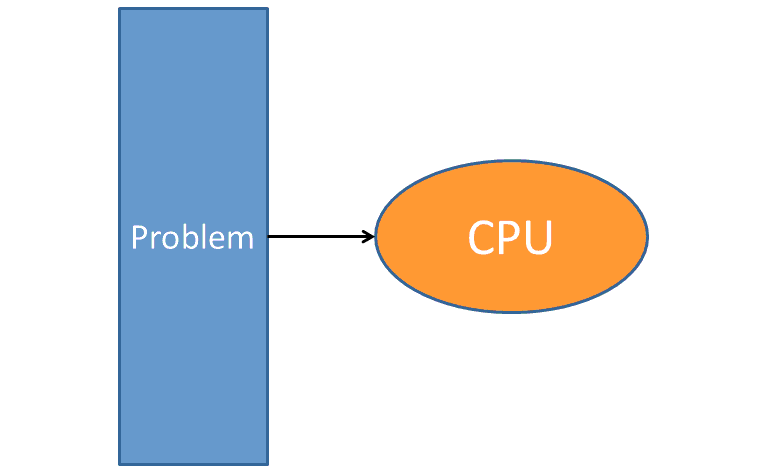
\includegraphics[width=.975\textwidth]{../common/pics/parallelism1}
      \end{center}
      \end{block}
    \end{minipage}
    \hspace{.15cm}
    \begin{minipage}{.46\textwidth}
    \begin{block}{\centering Parallel Programming}
      \begin{center}
      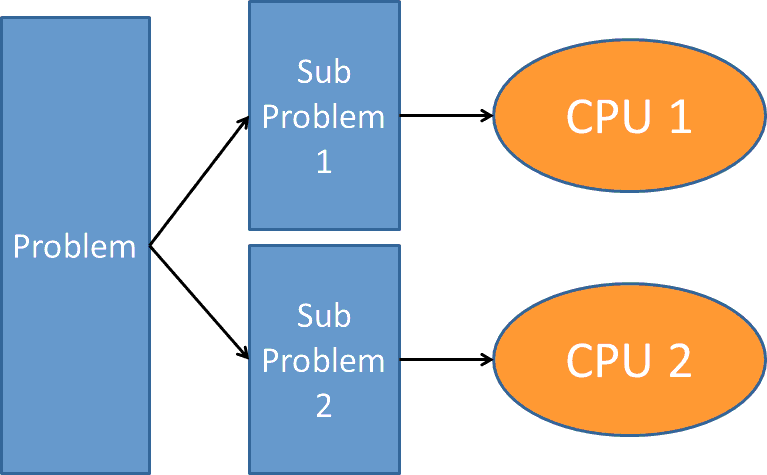
\includegraphics[width=.975\textwidth]{../common/pics/parallelism2}
      \end{center}
      \end{block}
    \end{minipage}
    \end{center}
  \end{block}
\end{frame}

\begin{frame}
  \begin{block}{Parallelism}\pause
    \begin{center}
    \begin{minipage}{.46\textwidth}
    \begin{block}{Serial Programming}
      \begin{center}
      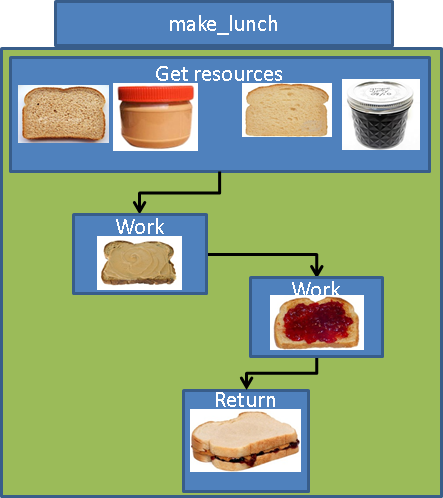
\includegraphics[width=.975\textwidth]{../common/pics/analogy_serial}
      \end{center}
      \end{block}
    \end{minipage}
    \hspace{.15cm}
    \begin{minipage}{.46\textwidth}
    \begin{block}{Parallel Programming}
      \begin{center}
      
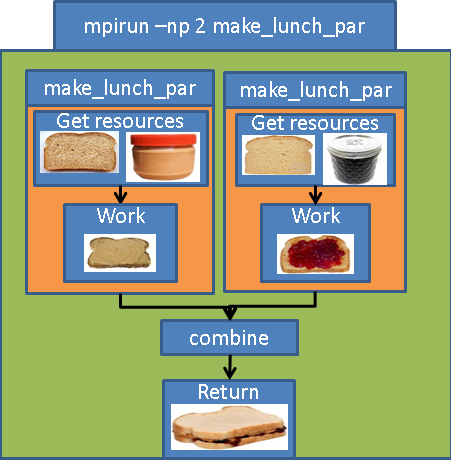
\includegraphics[height=5.45cm,width=.975\textwidth]{../common/pics/analogy_parallel}
      \end{center}
      \end{block}
    \end{minipage}
    \end{center}
  \end{block}
\end{frame}


\begin{frame}
  \begin{block}{Kinds of Parallelism}\pause
    \begin{itemize}[<+-|alert@+>]
      \item \emph{Data Parallelism}:  Data is distributed
      \item \emph{Task Parallelism}:  Tasks are distributed
  \end{itemize}
  (This is a gross oversimplification)
  \end{block}
\end{frame}


\begin{frame}
  \begin{block}{pbdR Paradigms:  Data Parallelism}
  Data parallelism:
  \begin{itemize}[<+-|alert@+>]
   \item No one processor/node owns all the data.
   \item Processors own local pieces of a (conceptually) larger, global object
  \end{itemize}
  
  Task parallelism:
  \begin{itemize}
    \item (Usually) Applying different tasks to the same data.
  \end{itemize}
  \end{block}
\end{frame}


\begin{frame}
  \begin{block}{Data vs Task Parallelism}\pause
    \begin{center}
    \begin{minipage}{.46\textwidth}
    \begin{block}{\centering Data Parallelism}
      \begin{center}
      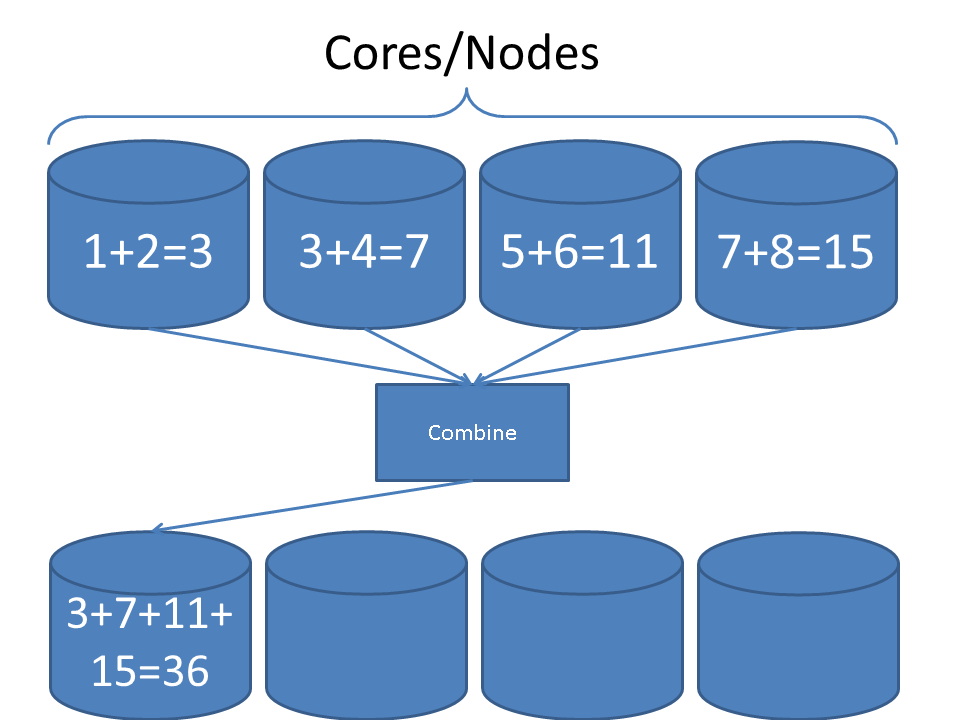
\includegraphics[width=.975\textwidth]{../common/pics/parallelism_data}
      \end{center}
      \end{block}
    \end{minipage}
    \hspace{.15cm}
    \begin{minipage}{.46\textwidth}
    \begin{block}{\centering Task Parallelism}
      \begin{center}
      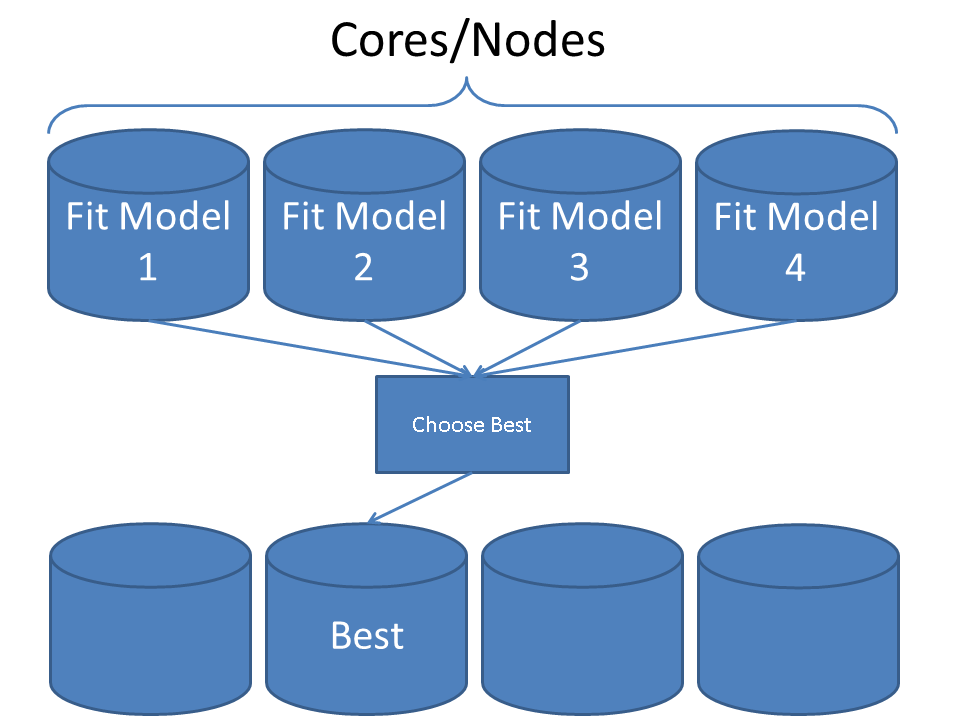
\includegraphics[width=.975\textwidth]{../common/pics/parallelism_task}
      \end{center}
      \end{block}
    \end{minipage}
    \end{center}
  \end{block}
\end{frame}




% \subsection{Common Terminology}


\begin{frame}
  \begin{block}{Parallel Programming Vocabulary:  Difficulty in Parallelism}
  \begin{enumerate}[<+-|alert@+>]
    \item \emph{Implicit parallelism}:  Parallel details hidden from user
    \item \emph{Explicit parallelism}:  Some assembly required\dots
    \item \emph{Embarrassingly Parallel}:  Also called \emph{loosely coupled}.  
Obvious how to make parallel; lots of independence in computations.
    \item \emph{Tightly Coupled}:  Opposite of embarrassingly parallel; lots of 
dependence in computations.
  \end{enumerate}  
  \end{block}
\end{frame}


\begin{frame}
  \begin{block}{Speedup}
  \begin{itemize}
    \item \emph{Wallclock Time}:  Time of the clock on the wall from start to 
finish
    \item \emph{Speedup}:  unitless measure of improvement; more is better.
  \begin{align*}
   S_{n_1, n_2} =  \frac{\text{Run time for } n_1 \text{ cores}}{\text{Run time 
for } n_2 \text{ cores}}
  \end{align*}
  \begin{itemize}
    \item   $n_1$ is often taken to be 1
    \item In this case, comparing parallel algorithm to serial algorithm
  \end{itemize}
  \end{itemize}
  \end{block}
\end{frame}


\begin{frame}
  \begin{block}{Speedup}
   \begin{center}
    \begin{minipage}{.475\textwidth}
    \begin{block}{Good Speedup}
      \centering
      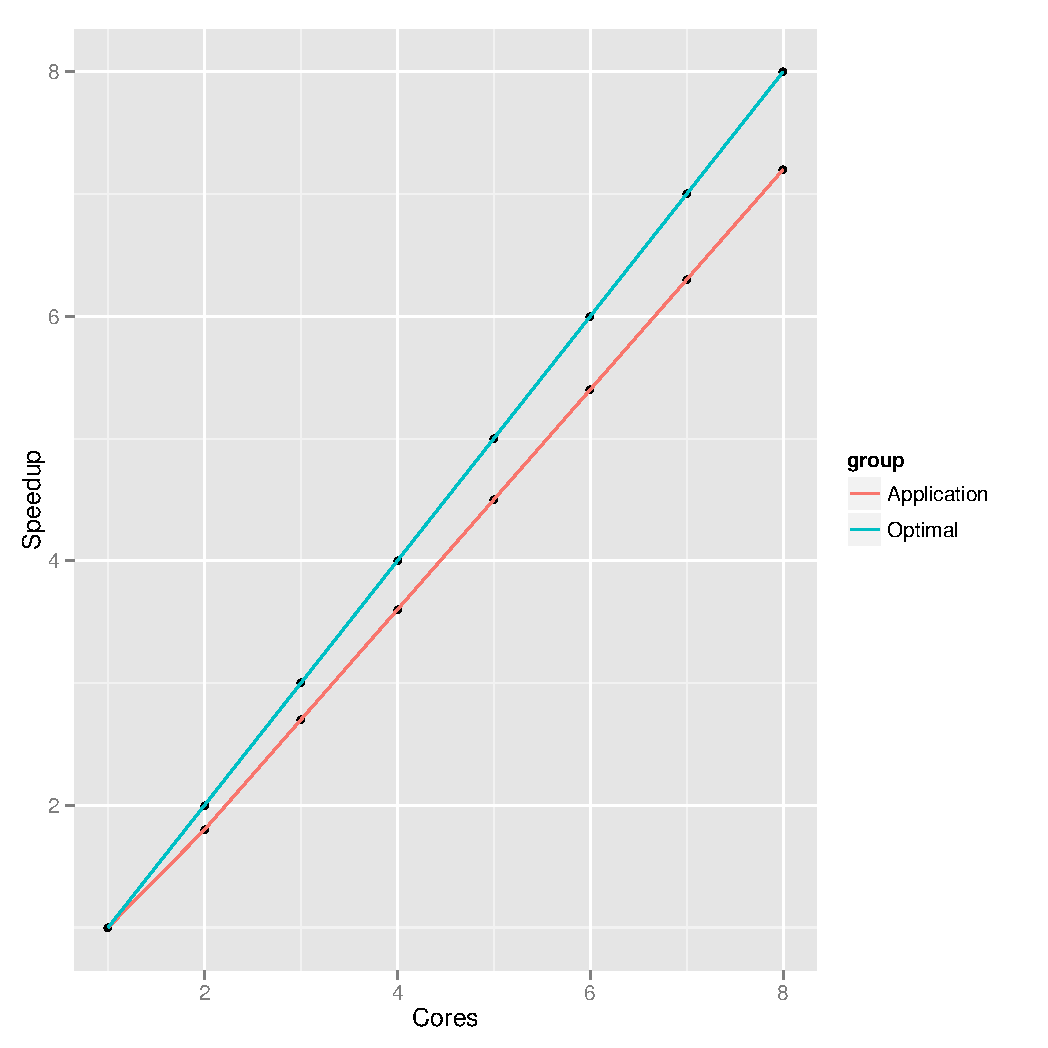
\includegraphics[width=.95\textwidth]{../common/pics/scale_good}
    \end{block}
    \end{minipage}
    \hspace{.1cm}
    \begin{minipage}{.475\textwidth}
    \begin{block}{Bad Speedup}
      \centering
      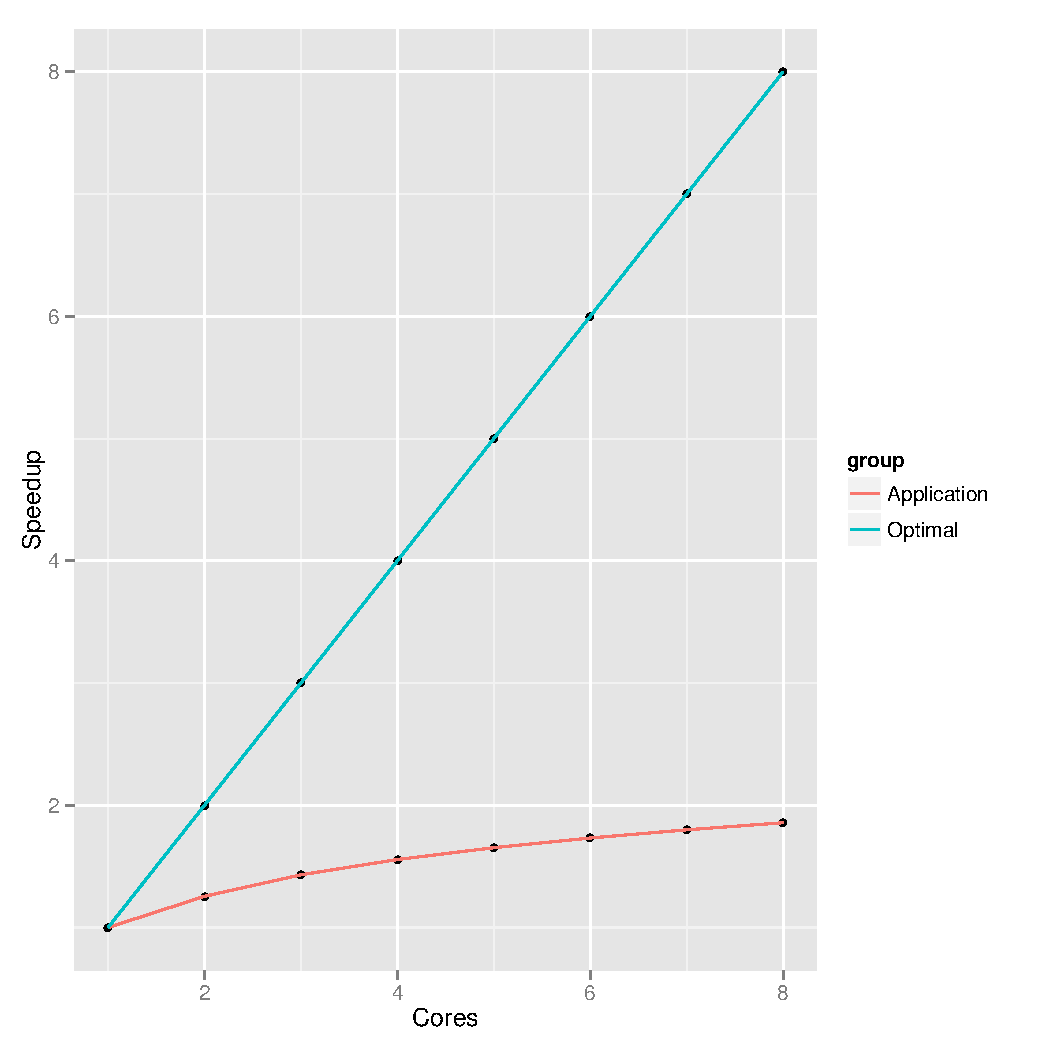
\includegraphics[width=.95\textwidth]{../common/pics/scale_bad}
    \end{block}
    \end{minipage}
    \end{center}
    \end{block}
\end{frame}


\begin{frame}
  \begin{block}{Shared and Distributed Memory Machines}
   \begin{center}
    \begin{minipage}{.475\textwidth}
    \begin{block}{Shared Memory}
     Direct access to read/change memory (one node) \vspace{.3cm} \ 
      \begin{center}
      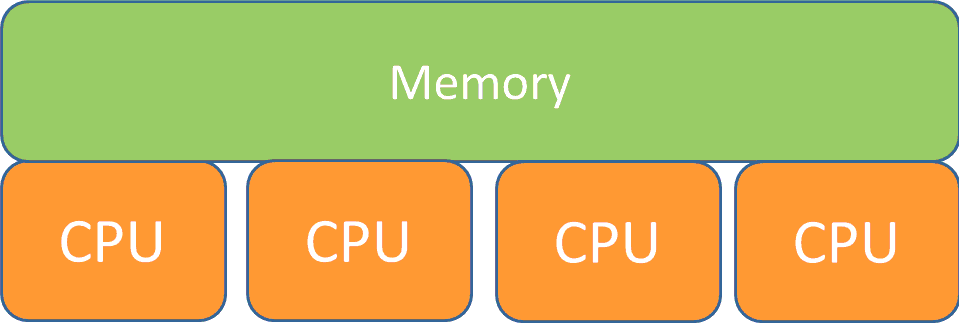
\includegraphics[width=.95\textwidth]{../common/pics/arch_shared}
      \end{center}
      \vspace{.3cm} \
    \end{block}
    \end{minipage}
    \hspace{.1cm}
    \begin{minipage}{.475\textwidth}
    \begin{block}{Distributed}
    No direct access to read/change memory (many nodes); requires communication
      \begin{center}
      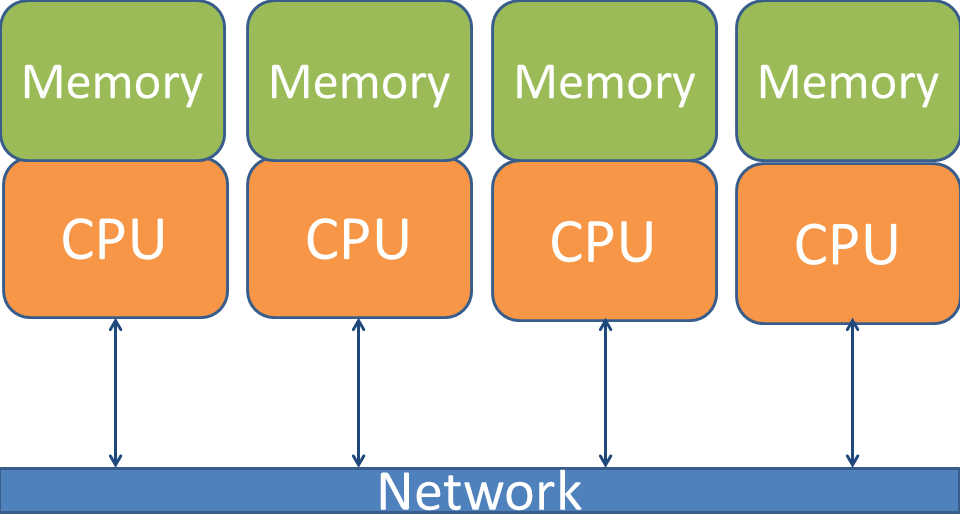
\includegraphics[width=.95\textwidth]{../common/pics/arch_distributed}
      \end{center}
    \end{block}
    \end{minipage}
    \end{center}
    \end{block}
\end{frame}


\begin{frame}
  \begin{block}{Shared and Distributed Memory Machines}
   \begin{center}
    \begin{minipage}[t]{.47\textwidth}
    \begin{block}{Shared Memory Machines}
    \begin{center}
    Thousands of cores\\[.2cm]
    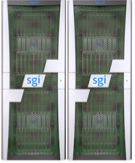
\includegraphics[scale=.65]{../common/pics/nautilus}\\
    {\tiny \emph{Nautilus}, University of Tennessee\\1024 cores \\4 TB RAM\\}
    \end{center}
    \end{block}
    \end{minipage}
    \hspace{.1cm}
    \begin{minipage}[t]{.47\textwidth}
    \begin{block}{Distributed Memory Machines}
    \begin{center}
    Hundreds of thousands of cores\\[.2cm]
    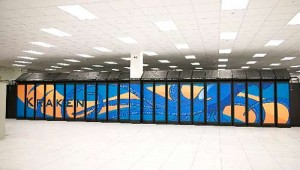
\includegraphics[width=.95\textwidth]{../common/pics/kraken}\\
    {\tiny \emph{Kraken}, University of Tennessee\\ 112,896 cores \\147 TB 
RAM\\}
    \end{center}
    \end{block}
    \end{minipage}
    \end{center}
    \end{block}
\end{frame}




\subsection{R and Parallelism}


\begin{frame}
%  \addtocounter{framenumber}{-1}
  \begin{block}{R and Parallelism}\pause
  What about R?
  \end{block}
\end{frame}

\begin{frame}
%  \addtocounter{framenumber}{-1}
  \begin{block}{Problems with Serial R}\pause
  \begin{enumerate}[<+-|alert@+>]
    \item Slow.
    \item If you don't know what you're doing, it's \emph{really} slow.
    \item Performance improvements usually for small machines.
    \item Very ram intensive.
  \end{enumerate}
  \end{block}
\end{frame}


\begin{frame}
  \begin{block}{Why We Need Parallelism}\pause
    \begin{enumerate}[<+-|alert@+>]
      \item Saves compute time.
      \item Data size is skyrocketing.
      \item Necessary for many problems.
      \item Its necessity is coming.
      \item \emph{It's really cool.}
  \end{enumerate}
  \end{block}
\end{frame}

\begin{frame}
  \begin{block}{Recall: Parallel R Packages}
   \begin{center}
    \begin{minipage}{.45\textwidth}
    \begin{block}{Shared Memory}
      \begin{enumerate}[<+-|alert@+>]
        \item \pkg{foreach}
        \item \pkg{parallel}
        \item \pkg{snow}
        \item \pkg{multicore}
      \end{enumerate}
    \end{block}
    \end{minipage}
    \hspace{.2cm}
    \begin{minipage}{.45\textwidth}
    \begin{block}{Distributed}
      \begin{enumerate}[<+-|alert@+>]
        \item \pkg{Rmpi}
        \item R+Hadoop
        \item \pkg{pbdR}
      \end{enumerate}
    \end{block}
    \end{minipage}
    \end{center}
    (and others\dots)
    \end{block}
\end{frame}



\begin{frame}[shrink]
  \begin{block}{R and Parallelism}
    The solution to many of R's problems is parallelism.  However \dots\vspace{-.4cm}
   \begin{center}
    \begin{minipage}[t]{.95\textwidth}
    \begin{block}{\centering What we have}
      \begin{enumerate}[<+-|alert@+>]
        \item Mostly serial.
        \item Mostly not distributed
        \item Data parallelism mostly explicit
      \end{enumerate}
    \end{block}
    \end{minipage}
    \\\pause
    \begin{minipage}[t]{.95\textwidth}
    \begin{block}{\centering What we want}
      \begin{enumerate}[<+-|alert@+>]
        \item Mostly parallel.
        \item Mostly distributed.
        \item Mostly implicit.
      \end{enumerate}
    \end{block}
    \end{minipage}
    \end{center}
    \end{block}
\end{frame}



\begin{frame}
  \begin{block}{R and Parallelism}
    Likewise, the HPC community is looking for high-level languages for data\dots
    \end{block}
\end{frame}


\section{Profiling and Benchmarking}
\makesubcontentsslides


%%% The need for profiling
\subsection{Why Profile?}
\makesubcontentsslidessec

\begin{frame}
  \begin{block}{Why Profile?}
  \begin{itemize}
    \item Because performance matters.
    \item Bad practices scale up!
    \item Your bottlenecks may surprise you.
    \item Because R is dumb.
  \end{itemize}
  \end{block}
\end{frame}


\begin{frame}[fragile]{Compilers often correct bad behavior\dots}
  \begin{center}
\begin{minipage}{.4\textwidth}
\vspace{0pt}
\begin{lstlisting}[title=A Really Dumb Loop,language=Rcpp]
int main(){
    int x, i;
    for (i=0; i<10; i++)
        x = 1;
    return 0;
}
\end{lstlisting}
\begin{lstlisting}[language=shl,title=clang -O3 example.c]
main:
        .cfi_startproc
# BB#0:
        xorl    %eax, %eax
        ret
\end{lstlisting}
\end{minipage}
\begin{minipage}{.57\textwidth}
\begin{lstlisting}[language=shl,title=clang example.c]
main:
        .cfi_startproc
# BB#0:
        movl    $0, -4(%rsp)
        movl    $0, -12(%rsp)
.LBB0_1:
        cmpl    $10, -12(%rsp)
        jge     .LBB0_4
# BB#2:
        movl    $1, -8(%rsp)
# BB#3:
        movl    -12(%rsp), %eax
        addl    $1, %eax
        movl    %eax, -12(%rsp)
        jmp     .LBB0_1
.LBB0_4:
        movl    $0, %eax
        ret
\end{lstlisting}
\end{minipage}

  \end{center}
\end{frame}



\begin{frame}[fragile]{R will not!}
    \begin{center}
\begin{minipage}[t]{.45\textwidth}
\begin{lstlisting}[title=Dumb Loop,escapeinside={(*@}{@*)}]


for (i in 1:n){
  Y <- (*@ \textcolor{red}{t(A)} @*) %*% Q
  Q <- qr.Q(qr(Y))
  Y <- A %*% Q
  Q <- qr.Q(qr(Y))
}

Q
\end{lstlisting}
\end{minipage}
\begin{minipage}[t]{.45\textwidth}
\begin{lstlisting}[title=Better Loop,escapeinside={(*@}{@*)}]
(*@ \textcolor{red}{tA <- t(A)} @*)

for (i in 1:n){
  Y <- tA %*% Q
  Q <- qr.Q(qr(Y))
  Y <- A %*% Q
  Q <- qr.Q(qr(Y))
}

Q
\end{lstlisting}
\end{minipage}
\end{center}
\end{frame}


\begin{frame}[fragile]{Example from a Real R Package}
    \begin{center}
\begin{minipage}[t]{.6\textwidth}
\vspace{-.9cm}
\begin{lstlisting}[title=Exerpt from Original function,escapeinside={(*@}{@*)}]
while(i<=N){
  for(j in 1:i){
    (*@ \textcolor{red}{d.k <- as.matrix(x)[l==j,l==j]}@*)
      ...
\end{lstlisting}
\vspace{-.3cm}
\begin{lstlisting}[title=Exerpt from Modified function,escapeinside={(*@}{@*)}]
(*@\textcolor{red}{x.mat <- as.matrix(x)}@*)

while(i<=N){
  for(j in 1:i){
    (*@ \textcolor{red}{d.k <- x.mat[l==j,l==j]}
@*)
      ...
\end{lstlisting}
\end{minipage}
\begin{minipage}[t]{.34\textwidth}
\vspace{1.1cm}
By changing just 1 line of code, performance of the main
method improved by \textbf{over 3.5$\times$} !
\end{minipage}
\end{center}
\end{frame}


\begin{frame}
  \begin{block}{Some Thoughts}
    \begin{itemize}
      \item R is slow.
      \item Bad programs are slower.
      \item High-level language: one line can touch a lot of data
      \item R will not fix bad programming
    \end{itemize}
  \end{block}
\end{frame}

\subsection{How to Profile and Benchmark}
\makesubcontentsslidessec

%%% Basic profiling
\begin{frame}[fragile]
  \begin{block}{Performance Profiling Tools: \code{system.time()}}
  \code{system.time()} is a basic R utility for timing expressions
\begin{lstlisting}[language=R]
x <- matrix(rnorm(20000*750), nrow=20000, ncol=750)

system.time(t(x) %*% x)
#    user  system elapsed 
#   2.187   0.032   2.324

system.time(crossprod(x))
#    user  system elapsed 
#   1.009   0.003   1.019 

system.time(cov(x))
#    user  system elapsed 
#   6.264   0.026   6.338 
\end{lstlisting}
  \end{block}
\end{frame}



\begin{frame}[fragile]
\begin{block}{Performance Profiling Tools: \code{Rprof()}}
\code{Rprof()} times the execution of all \R functions:
  \vspace{-.4cm}
\begin{lstlisting}[language=Rinteractive]
Rprof(filename="Rprof.out", append=FALSE, interval=0.02,
  memory.profiling=FALSE, gc.profiling=FALSE, 
  line.profiling=FALSE, numfiles=100L, bufsize=10000L)
\end{lstlisting}

\begin{lstlisting}[language=R]
x <- matrix(rnorm(10000*250), nrow=10000, ncol=250)

Rprof()
invisible(prcomp(x))
Rprof(NULL)

summaryRprof()

Rprof(interval=.99)
invisible(prcomp(x))
Rprof(NULL)

summaryRprof()
\end{lstlisting}
\end{block}
\end{frame}



\begin{frame}[fragile,shrink]
  \begin{block}{Performance Profiling Tools: \code{Rprof()}}
  \vspace{-.5cm}
\begin{lstlisting}[language=R]
$by.self
                self.time self.pct total.time total.pct
"La.svd"             0.68    69.39       0.72     73.47
"%*%"                0.12    12.24       0.12     12.24
"aperm.default"      0.04     4.08       0.04      4.08
"array"              0.04     4.08       0.04      4.08
"matrix"             0.04     4.08       0.04      4.08
"sweep"              0.02     2.04       0.10     10.20
### output truncated by presenter

$by.total
                 total.time total.pct self.time self.pct
"prcomp"               0.98    100.00      0.00     0.00
"prcomp.default"       0.98    100.00      0.00     0.00
"svd"                  0.76     77.55      0.00     0.00
"La.svd"               0.72     73.47      0.68    69.39
### output truncated by presenter

$sample.interval
[1] 0.02

$sampling.time
[1] 0.98
\end{lstlisting}
  \end{block}
\end{frame}



\begin{frame}[fragile]
  \begin{block}{Performance Profiling Tools: \code{Rprof()}}
  \vspace{-.5cm}
\begin{lstlisting}[language=R]
$by.self
[1] self.time  self.pct   total.time total.pct 
<0 rows> (or 0-length row.names)

$by.total
[1] total.time total.pct  self.time  self.pct  
<0 rows> (or 0-length row.names)

$sample.interval
[1] 0.99

$sampling.time
[1] 0
\end{lstlisting}
  \end{block}
\end{frame}



\begin{frame}[fragile]
  \begin{block}{Performance Profiling Tools: rbenchmark}
  \pkg{rbenchmark} is a simple package that easily benchmarks different 
functions:
\begin{lstlisting}[language=R]
x <- matrix(rnorm(10000*500), nrow=10000, ncol=500)

f <- function(x) t(x) %*% x
g <- function(x) crossprod(x)

library(rbenchmark)
benchmark(f(x), g(x))

#   test replications elapsed relative
# 1 f(x)          100  64.153    2.063
# 2 g(x)          100  31.098    1.000
\end{lstlisting}
  \end{block}
\end{frame}



%%% Advanced profiling
%\subsection{Advanced R Profiling}
\makesubcontentsslidessec

\begin{frame}
  \begin{block}{Other Profiling Tools}
    \begin{itemize}
      \item perf (Linux)
      \item PAPI
      \item MPI profiling: fpmpi, mpiP, TAU
    \end{itemize}
  \end{block}
\end{frame}


\begin{frame}[fragile]
  \begin{block}{Profiling MPI Codes with \textbf{pbdPROF}}
  \begin{minipage}[t]{.58\textwidth}
  \vspace{.2cm}
  \vspace{0pt}
  1. Rebuild \pbdR\ packages
\vspace*{-.5cm}
\begin{lstlisting}[language=shl,title=\ ]
R CMD INSTALL pbdMPI_0.2-1.tar.gz \ --configure-args= \ "--enable-pbdPROF"
\end{lstlisting}
2. Run code
\vspace*{-.5cm}
\begin{lstlisting}[language=shl,title=\ ]
mpirun -np 64 Rscript my_script.R
\end{lstlisting}

3. Analyze results
\vspace{-.5cm}
\begin{lstlisting}[title=\ ]
library(pbdPROF)
prof <- read.prof( "output.mpiP")
plot(prof, plot.type="messages2")
\end{lstlisting}

  \end{minipage}
  \hfill
  \begin{minipage}[t]{.4\textwidth}
  \vspace{0pt}
    \centering
    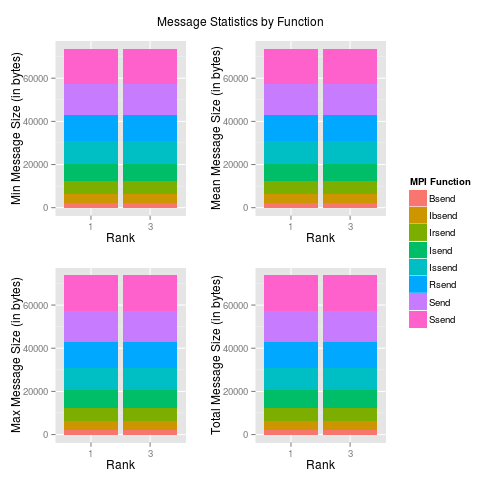
\includegraphics[scale=.25]{../common/pics/mpip}
    \\[.1cm]
    
\includegraphics[scale=0.35]{../common/pics/gsoc}
  \end{minipage}
  \end{block}
\end{frame}





\begin{frame}[fragile]
  \begin{block}{Profiling with \textbf{pbdPAPI}}
  \begin{minipage}{.6\textwidth}
    \begin{itemize}
      \item Performance Application Programming Interface
      \item High and low level interfaces
      \item Linux only :(
    \end{itemize}  
  \end{minipage}
  \begin{minipage}{.38\textwidth}
    \centering
    
\includegraphics[scale=0.12]{../common/pics/gsoc_2014}
  \end{minipage}
\begin{center}
\begin{tabular}{ll} \hline\hline
Function & Description of Measurement \\ \hline
\code{system.flips()} & Time, floating point instructions, and Mflips \\
\code{system.flops()} & Time, floating point operations, and Mflops \\
\code{system.cache()} & Cache misses, hits, accesses, and reads \\
\code{system.epc()} & Events per cycle \\
\code{system.idle()} & Idle cycles \\
\code{system.cpuormem()} & CPU or RAM bound$^*$ \\
\code{system.utilization()} & CPU utilization$^*$ \\
\hline\hline
\end{tabular}
\end{center}
  \end{block}
\end{frame}


\subsection{Summary}
\makesubcontentsslidessec


\begin{frame}[fragile]
  \begin{block}{Summary}\pause
    \begin{itemize}
      \item Start by loading the package:
\vspace{-.4cm}
\begin{lstlisting}
library(pbdMPI, quiet = TRUE)
\end{lstlisting}
      \item Always initialize before starting and finalize when finished:
\vspace{-.4cm}
\begin{lstlisting}
init()

# ...

finalize()
\end{lstlisting}
\end{itemize}
\end{block}
\end{frame}
\section{pbdR}
\makesubcontentsslides

\subsection{The pbdR Project}
\makesubcontentsslidessec

\begin{frame}{\pbdR Interfaces to Libraries: Sustainable Path}
  \vspace{-1ex}
  \centering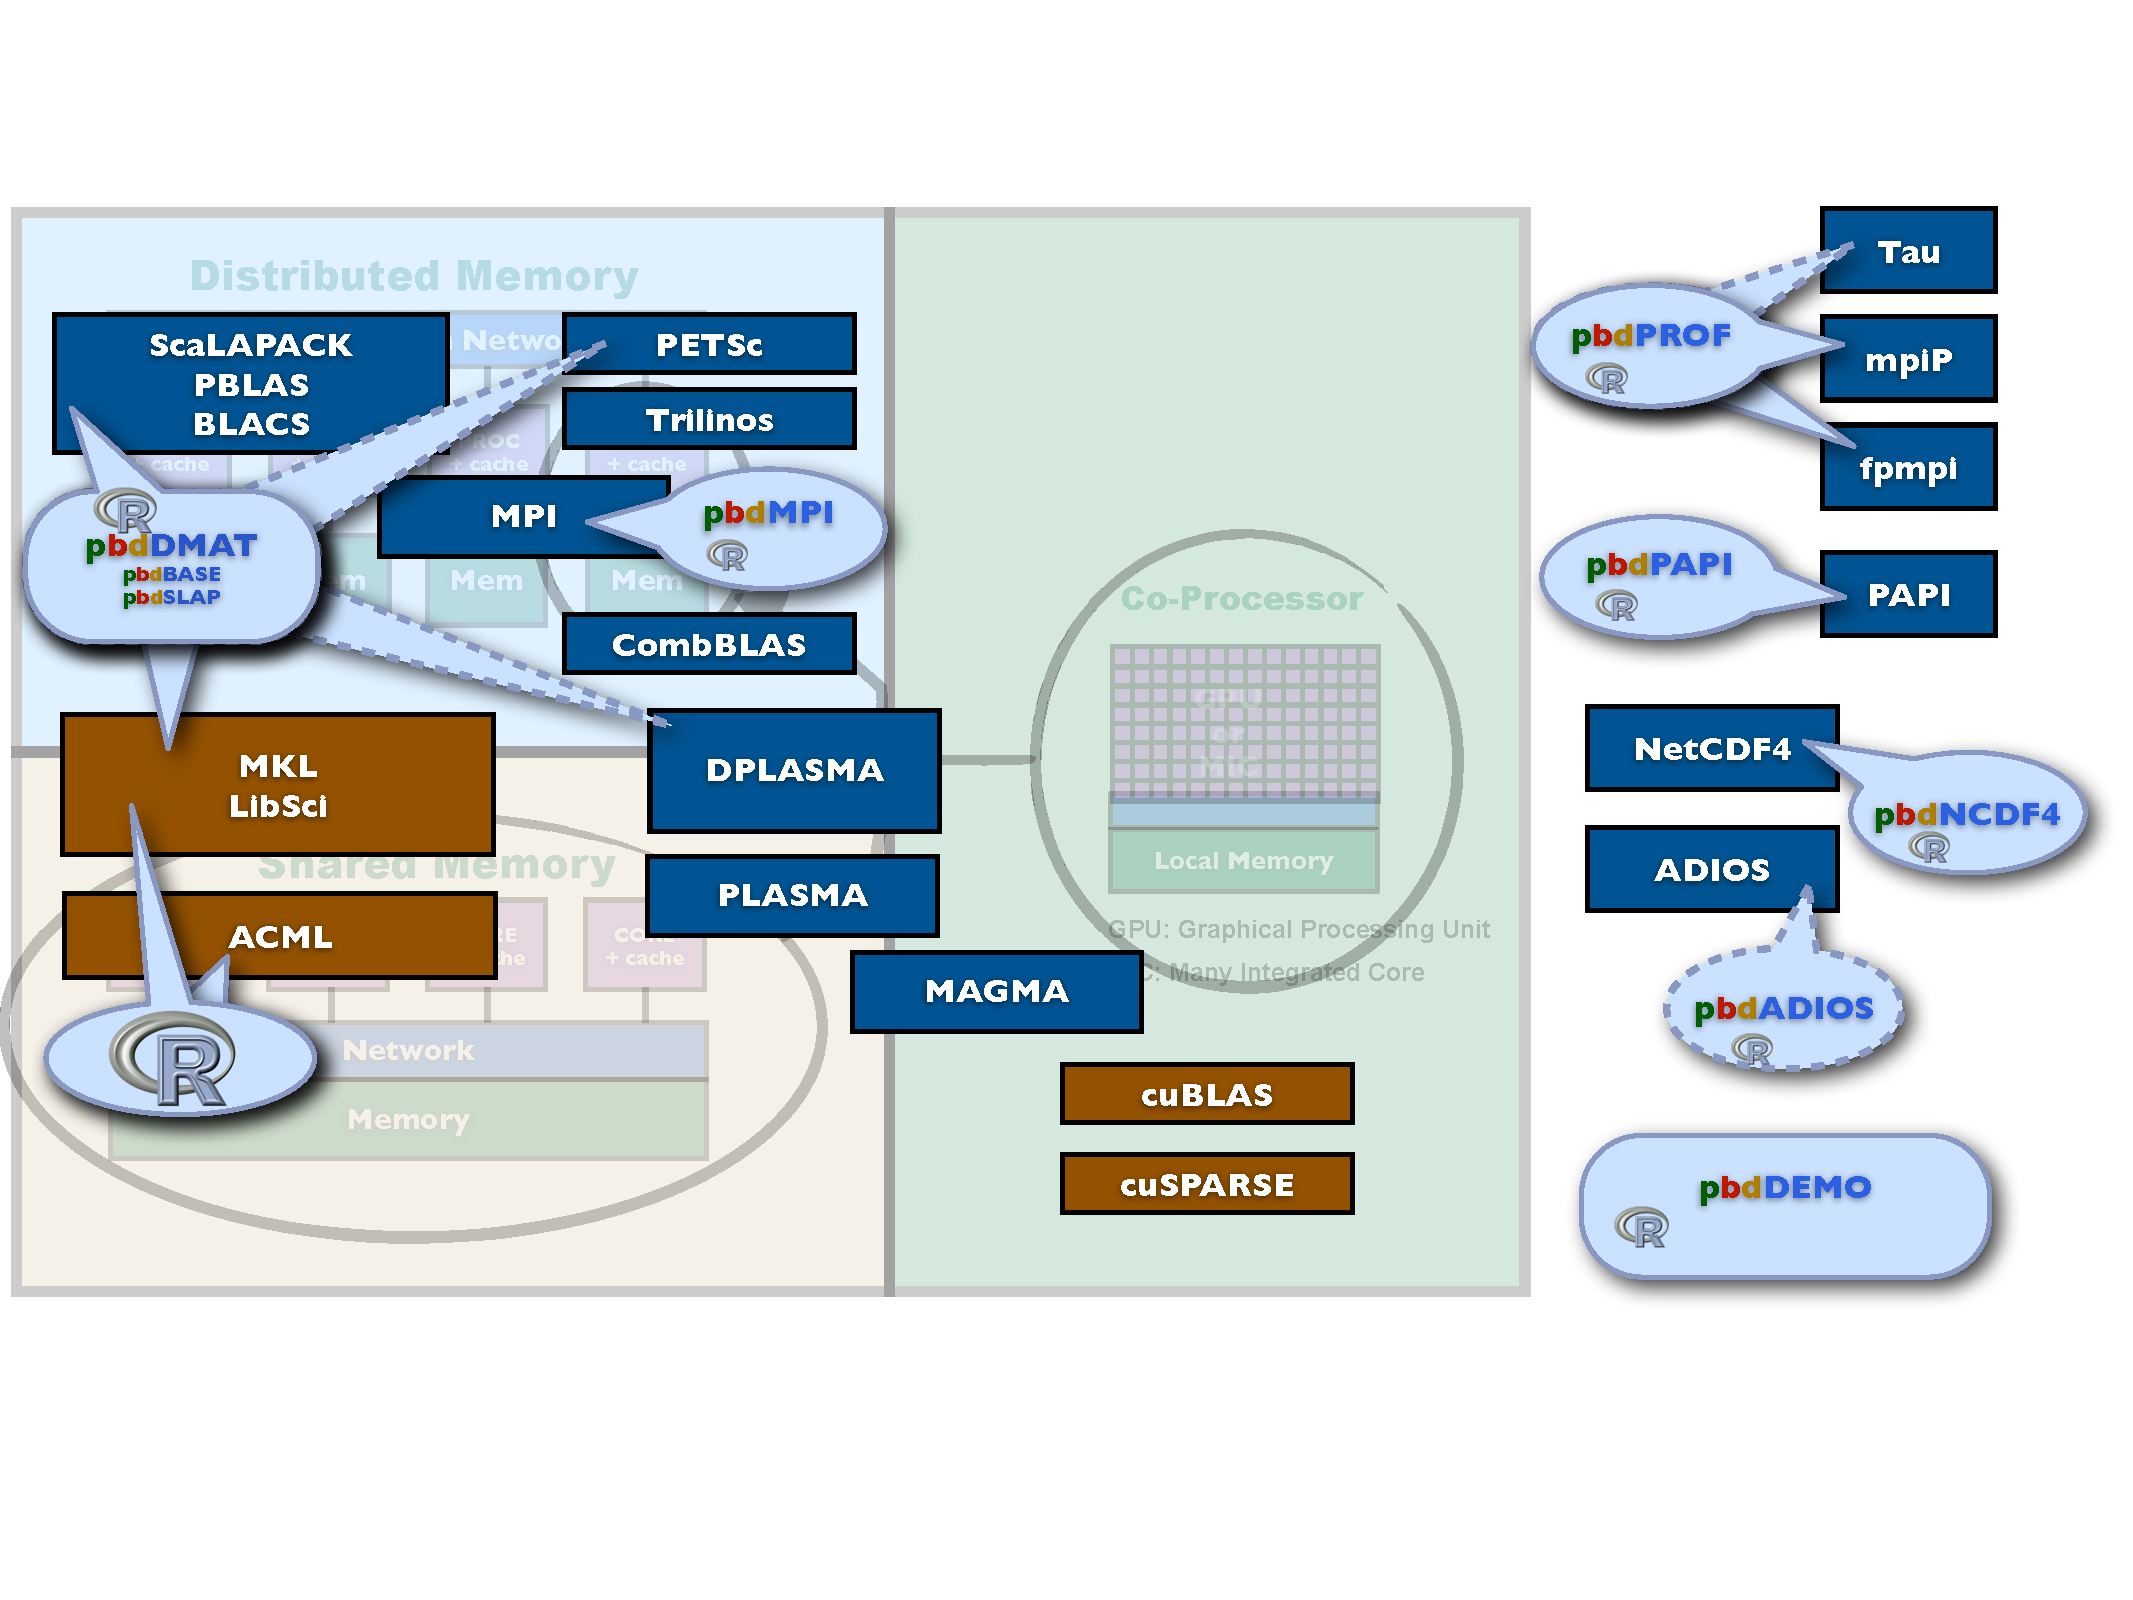
\includegraphics[trim=0cm 5cm 0cm 3cm,clip=true,width=0.85\textwidth]
  {../common/pics/hardware/ParallelHardware27.pdf}
  \scriptsize
  \begin{block}{Why use HPC libraries?}
    \begin{itemize}[<+-|alert@+>]
    \item The HPC community is 30 years beyond ``embarrassingly parallel.''
    \item \emph{They're tested.} \emph{They're
        fast.}  \emph{They're scalable.}
    \item Many science communities are invested in their API.
    \item Data analysis uses much of the same math as simulation science.
    \end{itemize}
  \end{block}
\end{frame}

\subsection{pbdMPI}
\makesubcontentsslidessec

\begin{frame}
  \begin{block}{pbdMPI: a High Level Interface to MPI}
    \begin{itemize}
    \item API is simplified: defaults in control objects.
    \item S4 methods: extensible to complex \R objects.
    \item Additional error checking
    \item Array and matrix methods without serialization: faster than
      \pkg{Rmpi}.
    \end{itemize}
    \begin{center}
      \vspace{0.2cm}\scriptsize
      \begin{tabular}{ll} \hline\hline
        \pkg{pbdMPI} (S4) & \pkg{Rmpi}                \\ \hline
        \code{\color{blue}allreduce}    & \code{mpi.allreduce}      \\
        \code{\color{blue}allgather}    & \code{mpi.allgather},
        \code{mpi.allgatherv},
        \code{mpi.allgather.Robj} \\
        \code{bcast}        & \code{mpi.bcast},
        \code{mpi.bcast.Robj}     \\
        \code{gather}       & \code{mpi.gather},
        \code{mpi.gatherv},
        \code{mpi.gather.Robj}    \\
        \code{recv}         & \code{mpi.recv},
        \code{mpi.recv.Robj}      \\
        \code{reduce}       & \code{mpi.reduce}         \\
        \code{scatter}      & \code{mpi.scatter},
        \code{mpi.scatterv},
        \code{mpi.scatter.Robj}   \\
        \code{send}         & \code{mpi.send},
        \code{mpi.send.Robj}      \\ \hline \hline
      \end{tabular}
    \end{center}
  \end{block}
\end{frame}

\begin{frame}[fragile]
  \begin{block}{Integer?\qquad Not always obvious in R.}
    \vspace{-.2cm}
    \begin{lstlisting}
> is.integer(1)
[1] FALSE
> is.integer(2)
[1] FALSE
> is.integer(1:2)
[1] TRUE
    \end{lstlisting}
  \end{block}
  \begin{block}{Often it's best to let the machine figure it out}\pause
    \begin{minipage}[t]{.475\textwidth}
      \begin{lstlisting}[title=Rmpi]
# int
mpi.allreduce(x, type=1)
# double
mpi.allreduce(x, type=2)
      \end{lstlisting}
    \end{minipage}
    \hfill
    \begin{minipage}[t]{.475\textwidth}
      \begin{lstlisting}[title=pbdMPI]
allreduce(x)
      \end{lstlisting}
      % \vspace{1em}
      % \hspace{1em}{\small S4. Batch only! (No spawning)}
    \end{minipage}
  \end{block}
\end{frame}



% \begin{frame}[fragile,shrink]
%   \begin{block}{Embarrassingly Parallel Computation}\pause
%     \vspace{-1ex}
%     \begin{minipage}[t]{.45\textwidth}
%       \begin{lstlisting}[title=EPforeach.R "asking for parallel",basicstyle=\tiny]
% library(doMPI, quiet=TRUE)
% cl <- startMPIcluster()
% registerDoMPI(cl)

% n <- 10
% myIn <- vector("list", n)

% myFun <- function(x) {
%   s <- sum(rnorm(10000))
%   rank <- mpi.comm.rank(comm=0)
%   return(paste(s, "from", rank))
% }

% results <- foreach(i = 1:n) %dopar% {
%   out <- myFun(myIn[[i]])
% }

% print(results)

% closeCluster(cl)
% mpi.quit()
%       \end{lstlisting}
%     \end{minipage}
%     \hfill
%     \begin{minipage}[t]{.5\textwidth}
%       \begin{lstlisting}[title=EPpbdR.R "thinking parallel",basicstyle=\tiny]
% library(pbdMPI, quiet=TRUE)
% init()

% myChunk <- get.jid(n <- 10)
% myIn <- vector("list", length(myChunk))
% myOut <- vector("list", length(myChunk))

% myFun = function(x) {
%   s <- sum(rnorm(10000))
%   rank <- comm.rank()
%   return(paste(s, "from", rank))
% }

% for(i in 1:length(myChunk)) {
%   myOut[[i]] <- myFun(myIn[[i]])
% }
% results <- gather(myOut)

% comm.print(results)
% finalize()
%       \end{lstlisting}
%     \end{minipage}
%   \end{block}
% \end{frame}


\begin{frame}[fragile]{SPMD Runs Many Copies of One Code}
  \begin{exampleblock}{SPMD Hello World: a ``map-reduce'' to all}
    \vspace{-1.5ex}
    \centering
    \begin{lstlisting}[title=map-reduce.r]
library(pbdMPI, quiet = TRUE)
init()

## Your "Map" code
n <- comm.rank() + 1

## Now "Reduce" but give the result to all
all_sum <- allreduce(n) # Sum is default

text <- paste("Hello: n is", n, "sum is", all_sum )
comm.print(text, all.rank=TRUE)

finalize()
    \end{lstlisting}
    \vspace{-4.5ex}
    \begin{columns}[t,onlytextwidth]
      \begin{column}{0.54\textwidth}
        \begin{lstlisting}[backgroundcolor=\color{white},keywordstyle=\color{black},
title=Execute this batch script via:]
mpirun -np 2 Rscript map-reduce.r
        \end{lstlisting}
      \end{column}
      \hfill
      \begin{column}{0.46\textwidth}
        \begin{lstlisting}[title=Output:]
COMM.RANK = 0
[1] "Hello: n is 1 sum is 3"
COMM.RANK = 1
[1] "Hello: n is 2 sum is 3"
        \end{lstlisting}
      \end{column}
    \end{columns}
  \end{exampleblock}
\end{frame}

\subsection{pbdDMAT}
\makesubcontentsslidessec

\begin{frame}{Dense Matrix and Vector Operations}
  \begin{block}{A matrix is mapped to a processor grid shape}
    \begin{table}[ht]
      \centering
      % \begin{subfigure}[b]{0.23\textwidth}
      %   \centering
      %   $\left[\begin{tabular}{l}
      %       0 \\ 1 \\ 2 \\ 3 \\ 4 \\ 5
      %     \end{tabular}\right]^T$
      %   \caption{$1\times 6$}
      % \end{subfigure}
      \begin{subfigure}[b]{0.23\textwidth}
        \centering
        $\left[\begin{tabular}{llllll}
            0 & 1 & 2 & 3 & 4 & 5
          \end{tabular}\right]$
        \vspace{1.5cm}
        \caption{$1\times 6$}
      \end{subfigure}%\hspace{-1cm}
      \begin{subfigure}[b]{0.23\textwidth}
        \centering
        $\left[\begin{tabular}{lll}
            0 & 1 & 2\\
            3 & 4 & 5
          \end{tabular}\right]$
        \caption{$2\times 3$}
      \end{subfigure}%
      \begin{subfigure}[b]{0.23\textwidth}
        \centering
        $\left[\begin{tabular}{ll}
            0 & 1 \\
            2 & 3\\
            4 & 5
          \end{tabular}\right]$
        \caption{$3\times 2$}
      \end{subfigure}
      \begin{subfigure}[b]{0.23\textwidth}
        \centering
        $\left[\begin{tabular}{l}
            0 \\ 1 \\ 2 \\ 3 \\ 4 \\ 5
          \end{tabular}\right]$
        \caption{$6\times 1$}
      \end{subfigure}
      \caption{Processor Grid Shapes with 6 Processors}\label{fig:gridshapes}
    \end{table}
  \end{block}
\end{frame}

\begin{frame}[shrink]
\begin{exampleblock}{2$\times$3 block-cyclic grid on 6 processors:
    Global view ``ddmatrix'' class}
\begin{align*}
x &= \left[
      \begin{array}{ll|ll|ll|ll|l}
      \color{g11}x_{11} & \color{g11}x_{12} & \color{g12}x_{13} & \color{g12}x_{14} & \color{g13}x_{15} & \color{g13}x_{16} & \color{g11}x_{17} & \color{g11}x_{18} & \color{g12}x_{19}\\
      \color{g11}x_{21} & \color{g11}x_{22} & \color{g12}x_{23} & \color{g12}x_{24} & \color{g13}x_{25} & \color{g13}x_{26} & \color{g11}x_{27} & \color{g11}x_{28} & \color{g12}x_{29}\\\hline
      \color{g21}x_{31} & \color{g21}x_{32} & \color{g22}x_{33} & \color{g22}x_{34} & \color{g23}x_{35} & \color{g23}x_{36} & \color{g21}x_{37} & \color{g21}x_{38} & \color{g22}x_{39}\\
      \color{g21}x_{41} & \color{g21}x_{42} & \color{g22}x_{43} & \color{g22}x_{44} & \color{g23}x_{45} & \color{g23}x_{46} & \color{g21}x_{47} & \color{g21}x_{48} & \color{g22}x_{49}\\\hline
      \color{g11}x_{51} & \color{g11}x_{52} & \color{g12}x_{53} & \color{g12}x_{54} & \color{g13}x_{55} & \color{g13}x_{56} & \color{g11}x_{57} & \color{g11}x_{58} & \color{g12}x_{59}\\
      \color{g11}x_{61} & \color{g11}x_{62} & \color{g12}x_{63} & \color{g12}x_{64} & \color{g13}x_{65} & \color{g13}x_{66} & \color{g11}x_{67} & \color{g11}x_{68} & \color{g12}x_{69}\\\hline
      \color{g21}x_{71} & \color{g21}x_{72} & \color{g22}x_{73} & \color{g22}x_{74} & \color{g23}x_{75} & \color{g23}x_{76} & \color{g21}x_{77} & \color{g21}x_{78} & \color{g22}x_{79}\\
      \color{g21}x_{81} & \color{g21}x_{82} & \color{g22}x_{83} & \color{g22}x_{84} & \color{g23}x_{85} & \color{g23}x_{86} & \color{g21}x_{87} & \color{g21}x_{88} & \color{g22}x_{89}\\\hline
      \color{g11}x_{91} & \color{g11}x_{92} & \color{g12}x_{93} & \color{g12}x_{94} & \color{g13}x_{95} & \color{g13}x_{96} & \color{g11}x_{97} & \color{g11}x_{98} & \color{g12}x_{99}\\
      \end{array}
\right]_{9\times 9}
\end{align*}
\begin{align*}
\text{Processor grid = }\left|
      \begin{array}{lll}
      \color{g11}0 & \color{g12}1 & \color{g13}2\\
      \color{g21}3 & \color{g22}4 & \color{g23}5
      \end{array}
\right| &=
\left|
      \begin{tabular}{lll}
      \color{g11}(0,0) & \color{g12}(0,1) & \color{g13}(0,2)\\
      \color{g21}(1,0) & \color{g22}(1,1) & \color{g23}(1,2)
      \end{tabular}
\right|
\end{align*}
\end{exampleblock}
\end{frame}


\begin{frame}[shrink]
\begin{exampleblock}{2$\times$3 block-cyclic grid on 6 processors:
    Local view ``ddmatrix'' class}
\begin{align*}
\left[
      \begin{array}{ll|ll}
      \color{g11}x_{11} & \color{g11}x_{12} & \color{g11}x_{17} & \color{g11}x_{18}\\
      \color{g11}x_{21} & \color{g11}x_{22} & \color{g11}x_{27} & \color{g11}x_{28}\\\hline
      \color{g11}x_{51} & \color{g11}x_{52} & \color{g11}x_{57} & \color{g11}x_{58}\\
      \color{g11}x_{61} & \color{g11}x_{62} & \color{g11}x_{67} & \color{g11}x_{68}\\\hline
      \color{g11}x_{91} & \color{g11}x_{92} & \color{g11}x_{97} & \color{g11}x_{98}\\
      \end{array}
\right]_{5\times 4}
\left[
      \begin{array}{ll|l}
      \color{g12}x_{13} & \color{g12}x_{14} & \color{g12}x_{19}\\
      \color{g12}x_{23} & \color{g12}x_{24} & \color{g12}x_{29}\\\hline
      \color{g12}x_{53} & \color{g12}x_{54} & \color{g12}x_{59}\\
      \color{g12}x_{63} & \color{g12}x_{64} & \color{g12}x_{69}\\\hline
      \color{g12}x_{93} & \color{g12}x_{94} & \color{g12}x_{99}\\
      \end{array}
\right]_{5\times 3}
\left[
      \begin{array}{ll}
      \color{g13}x_{15} & \color{g13}x_{16}\\
      \color{g13}x_{25} & \color{g13}x_{26}\\\hline
      \color{g13}x_{55} & \color{g13}x_{56}\\
      \color{g13}x_{65} & \color{g13}x_{66}\\\hline
      \color{g13}x_{95} & \color{g13}x_{96}\\
      \end{array}
\right]_{5\times 2}
\\
\left[
      \begin{array}{ll|ll}
      \color{g21}x_{31} & \color{g21}x_{32} & \color{g21}x_{37} & \color{g21}x_{38}\\
      \color{g21}x_{41} & \color{g21}x_{42} & \color{g21}x_{47} & \color{g21}x_{48}\\\hline
      \color{g21}x_{71} & \color{g21}x_{72} & \color{g21}x_{77} & \color{g21}x_{78}\\
      \color{g21}x_{81} & \color{g21}x_{82} & \color{g21}x_{87} & \color{g21}x_{88}\\
      \end{array}
\right]_{4\times 4}
\left[
      \begin{array}{ll|l}
      \color{g22}x_{33} & \color{g22}x_{34} & \color{g22}x_{39}\\
      \color{g22}x_{43} & \color{g22}x_{44} & \color{g22}x_{49}\\\hline
      \color{g22}x_{73} & \color{g22}x_{74} & \color{g22}x_{79}\\
      \color{g22}x_{83} & \color{g22}x_{84} & \color{g22}x_{89}\\
      \end{array}
\right]_{4\times 3}
\left[
      \begin{array}{ll}
      \color{g23}x_{35} & \color{g23}x_{36} \\
      \color{g23}x_{45} & \color{g23}x_{46} \\\hline
      \color{g23}x_{75} & \color{g23}x_{76} \\
      \color{g23}x_{85} & \color{g23}x_{86} \\
      \end{array}
\right]_{4\times 2}
\end{align*}
\begin{align*}
\text{Processor grid = }\left|
      \begin{array}{lll}
      \color{g11}0 & \color{g12}1 & \color{g13}2\\
      \color{g21}3 & \color{g22}4 & \color{g23}5
      \end{array}
\right| &=
\left|
      \begin{tabular}{lll}
      \color{g11}(0,0) & \color{g12}(0,1) & \color{g13}(0,2)\\
      \color{g21}(1,0) & \color{g22}(1,1) & \color{g23}(1,2)
      \end{tabular}
\right|
\end{align*}
\end{exampleblock}
\end{frame}

\begin{frame}[fragile]
  \begin{block}{\pbdR\ No change in syntax. \hfill Data redistribution functions.}
\vspace{-2ex}
  \begin{lstlisting}
x <- x[-1, 2:5]
x <- log(abs(x) + 1)
x.pca <- prcomp(x)
xtx <- t(x) %*% x
ans <- svd(solve(xtx))
  \end{lstlisting}
\vspace{-1ex}
  \begin{center}
  \emph{The above (and over 100 other functions) runs on 1 core with R \\
    or 10,000 cores with \pbdR ddmatrix class}
  \end{center}
\vspace{-2ex}
\begin{lstlisting}
> showClass("ddmatrix")
Class "ddmatrix" [package "pbdDMAT"]
Slots:
Name:     Data     dim    ldim   bldim   ICTXT
Class:  matrix numeric numeric numeric numeric
\end{lstlisting}
\vspace{-2ex}
\begin{lstlisting}
> x <- as.rowblock(x)
> x <- as.colblock(x)
> x <- redistribute(x, bldim=c(8, 8), ICTXT = 0)
\end{lstlisting}
  \end{block}
\end{frame}

\subsection{RandSVD}
\makesubcontentsslidessec


\begin{frame}[fragile]
\fontsize{8pt}{10}\selectfont
\begin{block}{Randomized truncated SVD\footnotemark}
  \begin{minipage}{.56\textwidth}
    \begin{center}
      \includegraphics[height=.41\textheight]{../common/pics/randsvd/randSVDalg}
      \\
      \includegraphics[height=.26\textheight]{../common/pics/randsvd/randSVDalg4_4}
    \end{center}
  \end{minipage}
%   \hspace{.01cm}
  \begin{minipage}{0.43\textwidth}
\begin{lstlisting}[title=Serial 
R,basicstyle=\tiny,backgroundcolor=\color{grayish} 
,numberstyle=\tiny\color{black},keywordstyle=\color{black},commentstyle=\color{ 
dkgreen},stringstyle=\color{black},escapeinside={(*@}{@*)}]
randSVD <- function(A, k, q=3)
  {
    ## Stage A
    Omega <- (*@ matrix(rnorm(n*2*k),@*)
      (*@ nrow=n, ncol=2*k) @*)
    Y <- A %*% Omega
    Q <- qr.Q(qr(Y))
    At <- t(A)
    for(i in 1:q)
      {
        Y <- At %*% Q
        Q <- qr.Q(qr(Y))
        Y <- A %*% Q
        Q <- qr.Q(qr(Y))
      }
    
    ## Stage B
    B <- t(Q) %*% A
    U <- La.svd(B)$u
    U <- Q %*% U
    U[, 1:k]
  }
\end{lstlisting} %balance$
\end{minipage}
{\fontsize{6pt}{10}\selectfont $^1$Halko, Martinsson, 
  and Tropp. 2011. Finding structure with randomness: probabilistic
  algorithms  for constructing \\[-1ex] approximate matrix decompositions
  \emph{SIAM Review} \textbf{53} 217--288}
\end{block}
\end{frame}


\begin{frame}[fragile]
 \fontsize{8pt}{10}\selectfont
\begin{block}{Randomized truncated SVD}
  \hfill
  \begin{minipage}{0.430\textwidth}
\begin{lstlisting}[title=Serial 
R,basicstyle=\tiny,backgroundcolor=\color{grayish} 
,numberstyle=\tiny\color{black},keywordstyle=\color{black},commentstyle=\color{ 
dkgreen},stringstyle=\color{black},escapeinside={(*@}{@*)}]
randSVD <- function(A, k, q=3)
  {
    ## Stage A
    Omega <- (*@ \textcolor{blue}{matrix(rnorm(n*2*k),} @*)
      (*@ \textcolor{blue}{ nrow=n, ncol=2*k)} @*)
    Y <- A %*% Omega
    Q <- qr.Q(qr(Y))
    At <- t(A)
    for(i in 1:q)
      {
        Y <- At %*% Q
        Q <- qr.Q(qr(Y))
        Y <- A %*% Q
        Q <- qr.Q(qr(Y))
      }
    
    ## Stage B
    B <- t(Q) %*% A
    U <- La.svd(B)$u
    U <- Q %*% U
    U[, 1:k]
  }
\end{lstlisting} %balance$
  \end{minipage}
  \hfill
  \begin{minipage}{0.430\textwidth}
\begin{lstlisting}[title=Parallel pbdR,basicstyle=\tiny,backgroundcolor=\color{
grayish}, numberstyle=\tiny\color{black},keywordstyle=\color{black},
commentstyle=\color{dkgreen},stringstyle=\color{black},escapeinside={(*@}{@*)}]
randSVD <- function(A, k, q=3)
  {
    ## Stage A
    Omega <- (*@ \textcolor{blue}{ddmatrix("rnorm",} @*)
      (*@ \textcolor{blue}{nrow=n, ncol=2*k)} @*)
    Y <- A %*% Omega
    Q <- qr.Q(qr(Y))
    At <- t(A)      
    for(i in 1:q)
      {
        Y <- At %*% Q   
        Q <- qr.Q(qr(Y))
        Y <- A %*% Q    
        Q <- qr.Q(qr(Y))
      }
    
    ## Stage B
    B <- t(Q) %*% A     
    U <- La.svd(B)$u 
    U <- Q %*% U     
    U[, 1:k]
  }
\end{lstlisting}  % balancing $
  \end{minipage}
\hfill
\end{block}
\end{frame}

\begin{frame}
  \begin{block}{From journal to scalable code and scaling data in one day.}
    \begin{center}
      \includegraphics[width=.4\textwidth]{../common/pics/randsvd/randSVDspeedup}
      \hspace{1cm}
      \includegraphics[width=.4\textwidth]{../common/pics/randsvd/randSpeedupSVD}
    \end{center}
  \end{block}
\end{frame}



\section[pbdMPI]{Introduction to pbdMPI}
\makesubcontentsslides


%%% MPI basics
\documentclass[a4paper,10pt]{article}
\usepackage[utf8]{inputenc}
\usepackage[margin=0.75in]{geometry}
\usepackage{hyperref}
% \usepackage{url}
\usepackage{color}
\usepackage{listings}
\usepackage{ifpdf}
\usepackage{graphicx}

\usepackage{caption}
\usepackage{subcaption}

\parskip 0pt
\parindent 0pt
% \renewcommand{\indent}{\hspace{2cm}}

\definecolor{gray}{rgb}{.6,.6,.6}
\definecolor{orange}{rgb}{1,0.5,0}
\definecolor{grayish}{rgb}{.775, .775, .775}

\definecolor{dkgreen}{rgb}{0,0.6,0}
\definecolor{mauve}{rgb}{0.58,0,0.82}

\lstdefinelanguage{sh}{basicstyle=\ttfamily\color{white}, backgroundcolor=\color{black}, breaklines=true} 

\ifpdf
\lstdefinelanguage{rr}{language=R, 
                       basicstyle=\ttfamily\color{black}, 
		       backgroundcolor=\color{grayish}, 
		       frame=single, 
		       breaklines=true, 
		       tabsize=2,
                      keywordstyle=\color{blue},
		      commentstyle=\color{dkgreen},
		      stringstyle=\color{mauve}
} 

\else

\lstdefinelanguage{rr}{basicstyle=\ttfamily\color{black}, 
		       backgroundcolor=\color{grayish}, 
		       frame=single, 
		       breaklines=true, 
		       tabsize=2
%                       keywordstyle=\color{blue},
% 		      commentstyle=\color{dkgreen},
% 		      stringstyle=\color{mauve}
} 

\fi


\lstnewenvironment{rr}{%
  \lstset{%
     language = R,%
      style    = default,%
    }%
 }{}





\hypersetup{
    pdfnewwindow=true,      % links in new window
    colorlinks=true,       % false: boxed links; true: colored links
    linkcolor=blue,          % color of internal links
    filecolor=blue,      % color of file links
    urlcolor=blue           % color of external links
}

\title{A Beginner's Guide to HPC with R on Nautilus}
\author{National Institute for Computational Sciences}

% \setcounter{secnumdepth}{0}

% \newcommand{\HRule}{\underline{\ \ \ \ \ \ \ \ \ \ \ \ \ \ \ \ \ \ \ \ }}
% \newcommand{\lsc}[1]{ \ \\ \ \\ \ \\ \ \\ \begin{flushright}\hyperlink{thetop}{Return to top} \end{flushright} \section{#1}}
\newcommand{\lsc}[1]{ \ \\ \section{#1}}
% \newcommand{\lsuc}[1]{ \ \\ \ \\ \begin{flushright}\hyperlink{thetop}{Return to top} \end{flushright} \subsection{#1}}
\newcommand{\lsuc}[1]{\subsection{#1}}

\begin{document}

\ifpdf \else
\Css{div.lstlisting{
    font-family: monospace;
    white-space: nowrap; margin-top:0.5em;
    margin-bottom:0.5em;
    color: black;
    background-color: gray;
  } 
  div.verbatim{
    font-family: monospace;
    white-space: nowrap; margin-top:0.5em;
    margin-bottom:0.5em;
    color: white;
    background-color: black;
  }
}


\Preamble{xhtml}
  \Configure{graphics*}  
         {pdf}  
         {\Needs{"convert \csname Gin@base\endcsname.pdf  
                               \csname Gin@base\endcsname.png"}%  
          \Picture[pict]{\csname Gin@base\endcsname.png}%  
         }  
\fi

\maketitle
\hypertarget{thetop}{\ }
\tableofcontents



%%%%%%%%%%%%%%%%%%%%%%%%%%%%%%%%%%%%%%%%%%%%%%%%%%%%%%%%%%%%%%%%%%%%%%%%%%%%%%%%%%%%%%%%%%%%%%%%%
%%%%%%%%%%%%%%%%%%%%%%%%%%%%%%%%%%%%%%%%%%%%%%%%%%%%%%%%%%%%%%%%%%%%%%%%%%%%%%%%%%%%%%%%%%%%%%%%%
%%%%%%%%%%%%%%%%%%%%%%%%%%%%%%%%%%%%%%%%%%%%%%%%%%%%%%%%%%%%%%%%%%%%%%%%%%%%%%%%%%%%%%%%%%%%%%%%%

\section{Introduction to HPC and Its View from R}
\makesubcontentsslides

\input{../common/01_introduction/hardware_short}

\input{../common/01_introduction/batch_interactive}

\subsection{Programming Models}
\makesubcontentsslidessec

\begin{frame}{Manager-Workers}
  \begin{block}{}
    \begin{itemize}
    \item A serial program (Manager) divides up work and/or data
    \item Workers run in parallel without interaction
    \item Manager collects/combines results from workers
    \item Divide-Recombine fits this model
    \end{itemize}
  \end{block}
\end{frame}

\begin{frame}{MapReduce}
  \begin{block}{}
    \begin{itemize}
    \item A concept born of a search engine
    \item Decouples certain coupled problems with an intermediate
      communication - shuffle
    \item User writes two serial codes: Map and Reduce
    \end{itemize}
  \end{block}
\end{frame}

\begin{frame}{MapReduce: a Parallel Search Engine Concept}
  \begin{block}{Search MANY documents \hfill Serve MANY users}
    \begin{center}\scriptsize
      \begin{equation*}
        \begin{array}{c@{\hspace{-2ex}}r@{\hspace{-2ex}}c}
          \begin{array}{c}
            \mbox{\scriptsize Web} \\
            \mbox{\scriptsize Pages} \\
            \mbox{\scriptsize (records)}
          \end{array} &
          \begin{array}{c}\tiny
            \\ \mbox{\tiny p0} \\ \mbox{\tiny p1} \\
            \mbox{\tiny p2} \\ \mbox{\tiny p3}
          \end{array} &
          \begin{array}{c}
            \mbox{\scriptsize Index Words (keys)} \\
            \left[
            \begin{array}{cccc}
              A_1 & A_2  & A_3 & A_4 \\
              \hline
              B_1 & B_2  & B_3 & B_4 \\
              \hline
              C_1 & C_2  & C_3 & C_4 \\
              \hline
              D_1 & D_2  & D_3 & D_4
            \end{array}
            \right]
          \end{array}
        \end{array}
        \hbox{\hspace{-2ex}}
        \begin{array}{c}
          \hbox{Shuffle} \\
          \longrightarrow \\
          \mbox{\code{MPI\_Alltoallv}}
        \end{array}
        \hbox{\hspace{-2ex}}
        \begin{array}{c@{\hspace{-2ex}}r@{\hspace{-2ex}}c}
          \begin{array}{c}
            \mbox{\scriptsize Index} \\
            \mbox{\scriptsize Words} \\
            \mbox{\scriptsize (keys)}
          \end{array} &
          \begin{array}{c}
            \\  \mbox{\tiny p0} \\ \mbox{\tiny p1} \\
            \mbox{\tiny p2} \\ \mbox{\tiny p3}
          \end{array} &
          \begin{array}{c}
            \mbox{\scriptsize Web Pages (records)} \\
            \left[
            \begin{array}{cccc}
              A_1 & B_1  & C_1 & D_1 \\
              \hline
              A_2 & B_2  & C_2 & D_2 \\
              \hline
              A_3 & B_3  & C_3 & D_3 \\
              \hline
              A_4 & B_4  & C_4 & D_4
            \end{array}
            \right]
          \end{array}
        \end{array}
      \end{equation*}
    \end{center}
    \vspace{2em}
    \begin{center}
      Matrix transpose in another language?
    \end{center}
  \end{block}
\end{frame}

\begin{frame}
  \begin{block}{Can use different sets of processors}
    \begin{center}
      \begin{equation*}\scriptsize
        \begin{array}{c@{\hspace{-2ex}}r@{\hspace{-2ex}}c}
          \begin{array}{c}
            \mbox{\scriptsize Web} \\
            \mbox{\scriptsize Pages} \\
            \mbox{\scriptsize (records)}
          \end{array} &
          \begin{array}{c}\tiny
            \\ \mbox{\tiny p0} \\ \mbox{\tiny p1} \\
            \mbox{\tiny p2} \\ \mbox{\tiny p3}
          \end{array} &
          \begin{array}{c}
            \mbox{\scriptsize Index Words (keys)} \\
            \left[
            \begin{array}{cccc}
              \\
              \hline
              B_1 & B_2  & B_3 & B_4 \\
              \hline
              \\
              \hline
              \\
            \end{array}
            \right]
          \end{array}
        \end{array}
        \hbox{\hspace{-2ex}}
        \begin{array}{c}
          \hbox{Streaming} \\
          \hbox{Shuffle} \\
          \longrightarrow \\
          \mbox{\code{MPI\_Scatter}}
        \end{array}
        \hbox{\hspace{-2ex}}
        \begin{array}{c@{\hspace{-2ex}}r@{\hspace{-2ex}}c}
          \begin{array}{c}
            \mbox{\scriptsize Index} \\
            \mbox{\scriptsize Words} \\
            \mbox{\scriptsize (keys)}
          \end{array} &
          \begin{array}{c}
            \\  \mbox{\tiny p4} \\ \mbox{\tiny p5} \\
            \mbox{\tiny p6} \\ \mbox{\tiny p7}
          \end{array} &
          \begin{array}{c}
            \mbox{\scriptsize Web Pages (records)} \\
            \left[
            \begin{array}{cccc}
              \quad  & B_1  & \quad & \quad \\
              \hline
              \quad  & B_2  & \quad  &  \quad \\
              \hline
              \quad  & B_3  & \quad  &  \quad \\
              \hline
              \quad  & B_4  & \quad  & \quad
            \end{array}
            \right]
          \end{array}
        \end{array}
      \end{equation*}
    \end{center}
  \end{block}
\end{frame}

\begin{frame}{MPI and MapReduce}
  \begin{block}{Both Concepts are about Communitation}
    \begin{itemize}
    \item One makes communication explicit, gives choices
    \item The other hides communication, gives one choice (shuffle)
    \end{itemize}
  \end{block}
\end{frame}

\begin{frame}{SPMD: Single Program Multiple Data}
  \begin{block}{}
    \begin{itemize}
    \item The prevalent way of distributed programming
    \item Can handle tightly coupled parallel computations
    \item It is designed for batch computing
    \item There is usually no manager - rather, all cooperate
    \item Prime driver behind MPI specification
    \end{itemize}
  \end{block}
\end{frame}

\begin{frame}{Early SPMD Work in Statistics: Crossproduct (Row-Block)}
  \includegraphics[width=\textwidth]
  {../common/pics/comm/Crossprod1987.png} \\
  \begin{block}{Hypercube: Individual send() and recv() over each dimension}
    {\scriptsize Ostrouchov (1987). Parallel Computing on a
      Hypercube: An overview of the architecture and some
      applications. {\em Proceedings of the 19th Symposium on the
        Interface of Computer Science and Statistics}, p.27-32.}
  \end{block}
\end{frame}

\begin{frame}{Simplified with MPI (and further with pbdMPI)}
  \includegraphics[trim=0cm 6cm 0cm 4cm,clip=true,width=\textwidth]
  {../common/pics/comm/ParallelHardware30.pdf}
  \vspace{-1ex}
  \begin{block}{Architecture-specific vendor optimizations}
    \begin{itemize}
    \item \small Cray MPT
    \item \small SGI MPT
    \end{itemize}
  \end{block}
\end{frame}

\begin{frame}{Data-flow: Parallel Runtime Scheduling and Execution
    Controller (PaRSEC)}
  \vspace{-.1cm}
  \hspace{2cm}\includegraphics[trim=0cm 0cm 0cm
  1cm,clip=true,width=7.5cm]{../common/pics/comm/PaRSEC1.png}
 \\[-3.4cm]
  \includegraphics[width=4cm]{../common/pics/comm/PaRSEC2.png}
  \hspace{5cm}{\tiny Graphic from icl.cs.utk.edu}
  \begin{block}
    {\tiny Bosilca, G., Bouteiller, A., Danalis, A., Faverge,
      M., Herault, T., Dongarra, J. "PaRSEC: Exploiting Heterogeneity
      to Enhance Scalability," IEEE Computing in Science and
      Engineering, Vol. 15, No. 6, 36-45, November, 2013.}
    \begin{itemize}\small
    \item Master data-flow controller runs distributed on all cores.
    \item Dynamic generation of current level in flow graph
    \item Effectively removes collective synchronizations
    \end{itemize}
  \end{block}
\end{frame}

\lsc{Interacting with Nautilus}
A complete set of documentation on connecting to Nautilus can be found at the \href{http://www.nics.tennessee.edu/getting-started/access}{the access page on the NICS site}.  We will provide some examples that should illustrate the process sufficiently for users, but if there is ambiguity, you are always encouraged to check the \href{http://www.nics.tennessee.edu}{NICS site} documentation.

\lsuc{Connecting to Nautilus}
In order to connect to and use Nautilus, you must have a \textbf{S}ecure \textbf{SH}ell (SSH) client.  SSH is a protocol that allows encrypted connections between remote computers.  It consists of two parts, the ssh server (Nautilus) and the ssh client (your computer).

\subsubsection{Connecting from Mac and Linux}\label{confml}
Mac OS X and Linux have a ssh client bundled with the operating system.  On a Mac, you can open a terminal by navigating to your Applications folder, then the Utilities folder, and running the app ``Terminal''.  On Linux, the method for starting a terminal will depend to some degree on your distribution of choice.\\\\
%
If you would prefer, you can also use Putty (see section \ref{confromwin} below) as it is multiplatform (although this is not necessary).  It provides a graphical user interface for starting (but not using) a terminal session.  For the remainder, we will not assume that you are using Putty (though if you are, it should be reasonably clear how to take the information here and use it appropriately in Putty; alternatively, see section \ref{confromwin} below).\\\\
%
For demonstration purposes, say your username for your Nautilus account is \texttt{nautuser}.  Exactly how you connect will depend on whether you have an XSEDE account or a Director's Discretion account from section \ref{getacct}.  If you have an XSEDE account, then you would enter into the terminal:
\begin{lstlisting}[language=sh]
ssh nautuser@login.nautilus.nics.xsede.org
\end{lstlisting}%%%
On the other hand, if you have a Director's Discretion account, you would login by entering into the terminal:
\begin{lstlisting}[language=sh]
ssh nautuser@login.nautilus.nics.tennessee.edu
\end{lstlisting}%%%

Of course, it is inconvenient to type this into the terminal every time, so you may wish to configure a ``shortcut'' of sorts.  To do this, you would need to create a file called \texttt{config} and put that in the \texttt{.ssh/} (note the preceding dot) subdirectory of your home directory.  If this directory does not exist, create it.  With your text editor of choice, you might enter into this config file:\\\\
%
\texttt{ Host nautilus\\
HostName login.nautilus.nics.xsede.org\\
User nautuser\\
TCPKeepAlive yes\\
}

filling in the appropriate information as needed, so that to connect you need only type
\begin{lstlisting}[language=sh]
ssh nautilus
\end{lstlisting}%%%
into the terminal.\\\\
%
However you choose to go about it, begin an ssh session with Nautilus.  On your first login, you will be prompted about adding a RSA key to your cache.  Do so.


See section \ref{nautpw} below for complete details about your password.

\subsubsection{Connecting from Windows}\label{confromwin}
Windows users will have to download an ssh client, such as \href{http://www.chiark.greenend.org.uk/~sgtatham/putty/}{Putty}.  For a complete set of Putty documentation, see \href{http://the.earth.li/~sgtatham/putty/0.62/htmldoc/}{the putty user manual}.\\\\
%
After starting putty, you will need to enter the Nautilus host name under the Session category.  Make sure that the connection type is set to SSH and that the port is 22.  Which host name you use will depend on which type of account you created in section \ref{getacct}.  If you have an XSEDE account, then you would use the hostname\\\\
%
\texttt{login.nautilus.nics.xsede.org}
\\\\
On the other hand, if you have a Director's Discretion account, you would login by entering into the terminal:\\\\
%
\texttt{login.nautilus.nics.tennessee.edu}
\\\\
You can save this session either as the default or under the name of your choosing.  There are many configurable options available to you in Putty, but they are not needed to proceed (though altering them may make your experience more enjoyable).\\\\
%
Your first time connecting you will be greeted with a warning about a secure RSA key.  Select the option to add the key to Putty's cache.  You will then be greeted by a prompt asking what name you wish to login as.  Enter the account name from the account creation step and press enter.  You will then be asked to enter your password.  See section \ref{nautpw} below for complete details about your password.

\subsubsection{Your Nautilus Password}\label{nautpw}
Your password for the Nautilus system will consist of two pieces:  your PIN that you set in the account creation process, and the number that shows on your NICS token.  For illustration, say your PIN is 1234 (do not make this your PIN) and your NICS token reads 567 890.  Then the password you would enter when prompted would be 1234567890.\\\\
%
The number displayed on your NICS token will change roughly every 30 seconds (the little bars on the lower left will give you a sense for how much longer you have with that particular set of digits).  For more information, see the \href{http://www.nics.tennessee.edu/getting-started/access#OTPAuthentication}{access page on the NICS site}.


\lsuc{Basic Commands}
Once you are connected to Nautilus, you will be greeted by a text prompt.  If this is your first interaction with such a system, you may have no idea how to proceed.  This part can be confusing at first, but with a little time and patience, it will become second nature to you.\\\\
%
When interacting with the shell, never forget that it is case sensitive.  The table below
\begin{table}[h]
 \centering
  \begin{tabular}{lll}\hline
   command & description & example\\\hline
   ls & list files in a directory & ls\\
   mkdir & make directory & mkdir dir\\
   cd & change directory & cd dir\\
   cp & copy a file & cp a b\\
   mv & move and/or rename a file & mv a dir\\
   man & the help system & man mv\\\hline       
  \end{tabular}
\end{table}  
provides the basic commands you will need most of the time.\\\\
%
Never be afraid to read the man pages.  If you ever find yourself wondering ``is it possible to'', the answer is yes, and it's probably an option explained in the man page for the program.  To search within a man page, use the \texttt{/} key followed by your query.  If there are multiple hits for your query, you can jump to the next one by pressing \texttt{n} and to the previous one with \texttt{N}.

  \lsuc{Loading Software}
Much of the software available on Nautilus must first be loaded by the user before it can be used.  If you enter the command
\begin{lstlisting}[language=sh]
R
\end{lstlisting}%%%
into the terminal (remember, case sensitive), you will get the message
\begin{lstlisting}[language=sh]
-bash:  R:  command not found
\end{lstlisting}%%%
assuming your shell is bash.  At any time you can see which shell you are using by entering the command
\begin{lstlisting}[language=sh]
file /bin/sh
\end{lstlisting}%%%
So how do we start R?  You must first load R through the module system.  To do so, you would enter the command
\begin{lstlisting}[language=sh]
module load r
\end{lstlisting}%%%
into the terminal, and R will now start as expected after entering the ``R'' command into the terminal.  You only have to use the module load command once per login session (but you must load R again after a disconnect).  
\begin{lstlisting}[language=sh]
module load r
R
\end{lstlisting}%%%`
The module system is very powerful and very important to your life on this (or any other) supercomputer.  Entering the command
\begin{lstlisting}[language=sh]
man module
\end{lstlisting}%%%
will give you a complete description of the functionality and use of the module system.  For more information, see the \href{http://www.nics.tennessee.edu/computing-resources/nautilus/software}{Nautilus software page on the NICS site}.\\\\
%
The table below summarizes the use of the module system.

\begin{table}[h]
 \centering
\begin{tabular}{ll}\hline
Command & Purpose\\\hline
module avail & List available programs in the module system\\
module load $<$program$>$ & Load program\\
module unload $<$program$>$ & Unload program\\\hline
% module swap $<$first$>$ $<$second$>$ & Swap first program for second (in cases of confli
\end{tabular}
\end{table}

\lsuc{Choosing a Text Editor}
Choosing a text editor can be a very lengthy journey, somewhat akin to seeking out religious enlightenment.  No one text editor is perfect, and a discussion of the features of common text editors is well beyond the scope of this document.  Eventually, you will likely want to choose use either \href{https://www.gnu.org/software/emacs/}{Emacs} (no relation to Apple) or \href{http://www.vim.org/}{vim}.  Each of these is available on Nautilus each time you log in (you do not have to load them through the module system).  If you are not familiar with either of these editors, they can be very difficult to learn at first, but learning to use one of these well is a good idea.\\\\
%
For now, these might be a bit intimidating and act as one more hurdle in getting to the real work you want to do.  To that end, it might be a good idea to start with a more friendly text editor, such as nano.  Nano is not loaded by default each session, so you will have to enter the command
\begin{lstlisting}[language=sh]
module load nano
\end{lstlisting}%%%
to first load nano, and then call the editor by entering
\begin{lstlisting}[language=sh]
nano
\end{lstlisting}%%%
The commands for nano are visible at the bottom of the screen.  So here, Ctrl together with R reads in a file, Ctrl together with O saves, etc.  The editor is extremely minimalistic in terms of features, but is a fine place to start until you become more comfortable working in a terminal. \\\\
If you wish to have nano loaded each time you log in to Nautilus, you could start nano, enter Ctrl+R to bring up the read file dialogue.  For the file, enter
\begin{lstlisting}[language=sh]
~/.bashrc
\end{lstlisting}%%%
and somewhere inside this configuration file, add the line
\begin{lstlisting}[language=sh]
module load nano
\end{lstlisting}%%%
Press Ctrl+O to save the edit, and whenever you log in from now on, you do not first have to first load nano through the module system to be able to run nano.

\lsuc{Transferring Files}
To transfer files over to Nautilus, you have a variety of options, explained in depth at the \href{http://www.nics.tennessee.edu/computing-resources/data-transfer}{Data Transfer page at the NICS site}.  For getting started, probably the two methods of file transfer available that will be of interest are sftp for small files and GridFTP for big files.

\subsubsection{Small File Transfer}
If the files you wish to transfer are not particularly large (eg, small datasets, some R scripts, etc.), probably the easiest way to proceed is to connect to Nautilus by sftp (the secure file transfer protocol).  \\\\
%
Mac and Linux users can use the terminal as with ssh, and Windows users can use Putty (via PSFTP) to connect via sftp.  Although there is gui program available for managing files over sftp called \href{http://filezilla-project.org/}{filezilla}.  If you elect to use filezilla, you should read its documentation, although the program should be fairly self-explanatory.\\\\
%
To connect from a terminal (Mac/Linux), you can enter the command \texttt{sftp} as you would use \texttt{ssh} in Section \ref{confml}.  So for example, you might enter the command
\begin{lstlisting}[language=sh]
sftp nautuser@login.nautilus.nics.xsede.org
\end{lstlisting}%%%
or if you set up your ssh config file as in the example, you could do
\begin{lstlisting}[language=sh]
sftp nautilus
\end{lstlisting}%%%
From here, you can transfer files via the self-explanatory commands \texttt{put} and \texttt{get}.  The above applies for Windows users, after you replace ``sftp'' with ``psftp''.\\\\
%
Your sftp password is the same as your ssh password. 

\subsubsection{Large File Transfer}
If you need to transfer large files, such as your full dataset, using sftp is not recommended.  In this case, the preferred method is GridFTP.  You will need a special GridFTP client such as \href{https://www.globusonline.org/}{globus-url-copyh} or \href{http://dims.ncsa.illinois.edu/set/uberftp/}{uberftp}.  For details about how to set up and use GridFTP with these clients, see the \href{http://www.nics.tennessee.edu/user-support/general-support/data-transfer/gridftp}{GridFTP page on the NICS site}.


\lsc{The Job Queue System}\label{jqssec}
Generally, you will do very little direct interaction with Nautilus.  You should not really be using Nautilus in the same way that you use a workstation; it is not a workstation.  Nautilus is a shared system.  No one person is the sole user of Nautilus at any given time (usually).  \\\\
%
The way you will want to run your analyses is by submitting your job to a queue system on Nautilus.  This system handles all of the user requests and keeps the various demands for resources (cores, ram) from different jobs from stepping on each others toes, so to speak.\\\\
%
A very thorough explanation of the various options and ways of interacting with the job queue system is provided at the \href{http://www.nics.tennessee.edu/computing-resources/nautilus/Batch_Scripts}{batch scripts page on the NICS site}, and so we will not reproduce that information here.  We merely provide a quick sketch of the general process.  For full details and explanations, see the NICS site.  However, you can find some example scripts in the Examples section, Section \ref{egsec}.\\\\
%
However, there are a few options which you should be made aware of.  First, processor allocations are given by node, not by core.  On Nautilus, there are 8 cores per node, so when requesting processors for your job, you should generally request multiples of 8 (because that is what you are going to get anyway).  If you request 1 core, you will get 8; requesting 9 gets you 16, etc.  Likewise, since allocations are by node, ram is allocated similarly.  Each node has 4gb of ram per cpu, and so if you request 8 cores, you will get 32gb of ram.\\\\
%
As for dealing with the queue system, the first step is usually to create an appropriate batch file for your particular job.  This batch file will contain the information Nautilus needs to run your job.  The kind of information you will need will depend on what kind of job you wish to submit.  See the examples in section \ref{egsec} as well as the \href{http://www.nics.tennessee.edu/computing-resources/nautilus/Batch_Scripts}{batch scripts page on the NICS site}.\\\\
%
Once you have your job file prepared, you can submit it to the queue using the \texttt{qsub} command.  So if you have a job file called \texttt{jobfile.pbs} prepared and you are in the directory of this file, then you can submit it to the queue system via the command
\begin{lstlisting}[language=sh]
qsub jobfile.pbs 
\end{lstlisting}%%%
You can check on your job via the commands \texttt{showq} and \texttt{qstat}, but will probably want to use the job file options to send out emails to you.\\\\
%
Finally, if you ever need to prematurely kill a job (whether it is running or merely queued), you can do so with the \texttt{qdel} command.
\lsc{R on Nautilus}
Performing an analysis with R on a remote system can be challenging at first.  The aim of this section is to help with the transition of specifically running R for analysis on a local desktop system to running R on a remote parallel system.

\lsuc{Packages and Libraries}

\subsubsection{Using the Existing Library}
Installing packages, especially complicated ones like Rmpi and gputools, can be difficult on a remote system, especially for the R user who may have never had to deal with compiling things before.  Thankfully, many of the packages you will want to use are already installed for you.  If we are using R version 2.12.0, then the default library path is
\begin{lstlisting}[language=sh]
/sw/analysis/r/2.12.0/sles11.1\_intel11.1/R-2.12.0/library} 
\end{lstlisting}%%%
So merely loading R via the module system and then, for instance, if you want to use the \texttt{multicore} library, since this is already in the default library, all you have to do is
\begin{lstlisting}[language=rr]
library(multicore)
\end{lstlisting}
If you require an additional package which is not currently installed, the simplest way to get this is to fill out a request at the \href{http://www.nics.tennessee.edu/software-request}{Request Software Installation page at the NICS site}.

\subsubsection{Managing Your Own R Library}
You can also of course manage your own R library, though for most this will at best be unnecessary, and at worst a needless, frustrating exercise.  If you do need to manage, at least in part, your own R library, then you must install packages from source, either by downloading the source package (say with the utility wget) and install it with the command
\begin{lstlisting}[language=sh]
R CMD INSTALL [options] packages
\end{lstlisting}%%%
or by using the \texttt{install.packages()} command in an interactive R session, setting the various options as needed (\texttt{lib=}, \texttt{INSTALL\_opts=}, \dots).  One option that is not optional (without overriding an R environment variable; see paragraph to follow for details) when installing a package to a custom, user-managed library is the \texttt{lib=} argument.  This is so because you do not have write access to your default library.  Similarly, to load a package from a custom library, make sure you set the appropriate \texttt{lib.loc=} argument when issuing the \texttt{library()} command in R.\\\\
%
One additional note to consider when maintaining your own R package library is that you will likely need to manually set a few R environment variables in order to get some packages to install, or even load.  For a mostly complete list of R environment variables, enter the command \texttt{help("environment variables")} in an interactive R session.

\lsuc{Different R Versions}
For more information, see the \href{http://www.nics.tennessee.edu/computing-resources/nautilus/software?&software=r}{R page at the NICS site}.

\lsuc{Running Batch Jobs}
As mentioned in Section \ref{jqssec}, you generally should not be running R in quite the same way that you would run it on your workstation.  On your workstation, you probably use R interactively; that is, you load up an R session and submit lines to the R terminal as you need. \\\\
%
By contrast, on Nautilus, you will be running R scripts in batch.  That is, you will not start an interactive R session.  Instead, you will issue a command from the terminal (really, from you job script) to start R, run your analysis, direct output to a file, and kill R when the script completes (or encounters an error).  Now, for the purposes of appropriate resource allocation, this should be be done in your jobfile that you submit via qsub, rather than directly handled in the terminal.  This is merely intended to illustrate what is actually going on.  \\\\
%
One way to do this is to issue the terminal command \texttt{R CMD BATCH}.  So say the script you wish to have R run is called \texttt{myscript.R}.  Then issuing the command
\begin{lstlisting}[language=sh]
R CMD BATCH myscript.R 
\end{lstlisting}%%%
will run the \texttt{myscript.R} script through R in a way that is somewhat equivalent to starting an interactive R session and issuing the R commands 
\begin{lstlisting}[language=rr]
sink("myscript.Rout")
source("myscript.R")
q(save="no")
\end{lstlisting}

% \lsuc{Starting an interactive R session}
% Most of the time when you use R on Nautilus, you should submit a batch job via the queue system.  However, on occasion you may need to run R interactively (like you would on your own computer).  

% \input{05{parallelr}
% 
\lsc{Examples}\label{egsec}
  \lsuc{A Monte Carlo Simulation}
You are probably familiar with the Monty Hall problem from the game show Let's Make a Deal.  If not, you might wish to read the \href{https://en.wikipedia.org/wiki/Monty_Hall_problem}{Wikipedia page} devopted to this problem.  A brief explanation is that the contestant is shown three doors to choose between.  Behind only one door is a prize.  The contestant chooses a door, and from the unchosen 2 doors, one is removed from play.  The contestant is then asked if he or she would like to switch from the initially chosen door to the only remaining door.  What is the probability of winning if the contestant switches?\\\\
%
We can easily simulate a play of this game with the R function \texttt{f()} defined as
\begin{lstlisting}[language=rr]
# Single game, assuming the player always switches
f <- function(.){
  prize.door <- sample(1:3, size=1)
  choice <- sample(1:3, size=1)

  if (choice==prize.door) return(0) else return(1) # Always switch
}
\end{lstlisting}

This is not necessarily the most efficient way to proceed.  Generally calling functions is costly, so it might make more sense to develop \texttt{f()} to take a ``number of runs'' argument, and this would probably improve the performance somewhat.  However, proceeding in our fashion is, for the sake of example, somewhat easier to follow in the various parallel implementations.

\subsubsection{Serial}
With the function \texttt{f} as above, it we can use \texttt{lapply()} to evaluate many runs
\begin{lstlisting}[language=rr]
n <- 1e7 # number of trials

system.time({
  mean(unlist(lapply(X=1:n, FUN=f)))
})
\end{lstlisting}
If this code is stored in the file serial.R, then you might submit it to Nautilus via the job file (remember to change ``your-account-number'' below to your actual account number.  Use the command \texttt{showusage}):
\begin{lstlisting}[language=sh]
#PBS -N Serial_sim_example
#PBS -S /bin/bash
#PBS -A your-account-number
#PBS -j oe
#PBS -l ncpus=8
#PBS -l walltime=1:00:00
#PBS -q analysis

module load r

R CMD BATCH serial.R
\end{lstlisting}%%%
Notice that we are asking for 8 cores, even though we are only going to use 1.  Remember that asking for 1 really takes 8 anyway.\\\\
%
Submitting this job results in the run time:
\begin{lstlisting}[language=rr]
   user  system elapsed 
187.275   0.220 187.516 
\end{lstlisting}


\subsubsection{Multicore}
With multicore, there is not much that we have to change over the serial implementation
\begin{lstlisting}[language=rr]
n <- 1e7 # number of trials
cores <- 10 # number of cores

library(multicore)

system.time({
  # mclapply() instead of lapply()
  mean(unlist(mclapply(X=1:n, FUN=f, mc.cores=cores)))
})
\end{lstlisting}

The \texttt{mclapply()} functions has the option \texttt{set.seed=} which defaults to \texttt{TRUE}.  This ensures that parallel processes have different seeds, which of course is very important for Monte Carlo simulation, since otherwise independence of the trials is violated.\\\\
%
If this code is stored in the file multicore.R, then you might submit it to Nautilus via the job file:

\begin{lstlisting}[language=sh]
#PBS -N Multicore_sim_example
#PBS -S /bin/bash
#PBS -A your-account-number
#PBS -j oe
#PBS -l ncpus=8
#PBS -l walltime=1:00:00
#PBS -q analysis

module load r
export TMPDIR=$HOME
export LC_ALL=C

cd $PBS_O_WORKDIR
R CMD BATCH multicore.R
\end{lstlisting}%%%
Submitting this job results in the run time:
\begin{lstlisting}[language=rr]
   user  system elapsed 
162.329   2.208  61.459 
\end{lstlisting}


\subsubsection{SNOW}
\begin{lstlisting}[language=rr]
n <- 1e7 # number of trials
cores <- 10 # number of cores

library(rlecuyer) # for parallel rng
library(snow)

system.time({
  # set up the workers
  cl <- makeCluster(cores, type="SOCK")
  
  # Pass objects to the workers
  clusterExport(cl, c("n", "cores", "f"))

  # parLapply() instead of lapply()
  mean(unlist(parLapply(cl=cl, x=1:n, fun=f)))
  stopCluster(cl)
})
\end{lstlisting}

If this code is stored in the file snow.R, then you might submit it to Nautilus via the job file:

\begin{lstlisting}[language=sh]
#PBS -N SNOW_sim_example
#PBS -S /bin/bash
#PBS -A your-account-number
#PBS -j oe
#PBS -l ncpus=8
#PBS -l walltime=1:00:00
#PBS -q analysis

module load r

R CMD BATCH snow.R
\end{lstlisting}%%%
Submitting this job results in the run time:
\begin{lstlisting}[language=rr]
   user  system elapsed 
 86.069   2.720 124.031 
\end{lstlisting}


\subsubsection{Rmpi}
Generally speaking, Rmpi is a bit trickier.  MPI is very powerful, and with that power comes a slightly more complicated API than with those above.  Since Nautilus is a shared memory machine, there is no real advantage to using Rmpi over Multicore; generally you should expect the runtimes to roughly be the same.  However, if you are on a distributed memory cluster, then there is only so much you can do with Multicore.  \\\\
%
Multicore operates on one node, with as many cores used within that node as possible/requested.  Nautilus is basically one big node, so Multicore can utilize all of its cores.  On a distributed memory cluster, this is not so, and the number of cores that can be utilized by Multicore will be significantly lower than can be utilized by Rmpi, and whence the potential speedup gained by Multicore on such systems pales in comparison for very big jobs.\\\\
%
Here there is a very important difference over Multicore and SNOW.  We \emph{must} make explicit steps to ensure that the random number generation operates appropriately on the workers.  Here, we do so with the \href{http://cran.r-project.org/web/packages/rlecuyer/index.html}{rlecuyer} package for R.  This can also be done with the \href{http://cran.r-project.org/web/packages/rsprng/index.html}{rsprng} package.\\\\
%
Here for consistency with the previous examples, we will use \texttt{mpi.parLapply()}, though arguably \texttt{mpi.parSim()} is more appropriate.  \\\\
%
See the \href{http://cran.r-project.org/web/packages/Rmpi/Rmpi.pdf}{rmpi documentation} for more details about the Rmpi API.
\begin{lstlisting}[language=rr]
n <- 1e7 # number of trials

library(rlecuyer) # for parallel rng
library(Rmpi)

system.time({
  mpi.spawn.Rslaves(needlog = FALSE)

  # set up parallel rng on the slaves
  mpi.setup.rngstream() 

  # mpi.parLapply() instead of lapply()
  mean(unlist(vec <- mpi.parLapply(x=1:n, fun=f)))
})

mpi.close.Rslaves(dellog = FALSE)
mpi.exit()
\end{lstlisting}

If this code is stored in the file rmpi.R, then you might submit it to Nautilus via the job file:

\begin{lstlisting}[language=sh]
#PBS -N Rmpi_sim_example
#PBS -S /bin/bash
#PBS -A your-account-number
#PBS -j oe
#PBS -l ncpus=8
#PBS -l walltime=1:00:00
#PBS -q analysis

module load r
module swap mpt mpt/2.04
export LC_ALL=C
export TMPDIR=$PBS_O_WORKDIR

cd $PBS_O_WORKDIR
mpirun -np 8 Rscript rmpi.R
\end{lstlisting}%%%
Submitting this job results in the run time:
\begin{lstlisting}[language=rr]
   user  system elapsed 
 99.370   1.088 100.581 
\end{lstlisting}


\lsuc{Linear Model Selection}
For the remainder, example job scripts will be suppressed, since they are effectively the same as those found in the examples above.\\\\
%
In this example, we will randomly generate a random normal response variable $y$, 10 random normal predictor variables $x$ and evaluate all possible $2^{10} -1 = 1023$ models which contain at least one predictor variable and choose a best model by the \href{https://en.wikipedia.org/wiki/Bayesian_information_criterion}{Bayesian Information Criterion}.\\\\
%
First we need to generate the data.  Since this is not the focus of this demonstration, we will do it once, independent of the parallel implementation.  
\begin{lstlisting}[language=rr]
n <- 1e7 # number of rows to generate

# The data
nvars <- 10
x <- matrix(rnorm(n*nvars), ncol=nvars)
y <- rnorm(n)

write.csv(data.frame(x, y), "simdata.csv")
\end{lstlisting}
A quick word of warning, it is possible that some of the models will have infinite likelihood, and no extra precaution is taken in the code to follow to prevent such an occurrence.  If you are getting strange errors, try generating a new dataset.  \\\\
%
Once this dataset has been generated, we can use the same simulated data each time in our testing of various parallel implementations.

\subsubsection{Serial}
Here, we will just have a single \texttt{for} loop that will run through the models one at a time.  This is not necessarily efficient, even ignoring running things in parallel, but this is the simplest way one might prototype a solution to this problem.  \\\\
%
For each model to be evaluated, the model is fit and its BIC score is calculated.  A comparison is made to that BIC score and the yet lowest observed BIC, and if the model BIC is lower than the previous best BIC, then we make that model the new best.

\begin{lstlisting}[language=rr]
# Read in the data
df <- read.csv("simdata.csv")
x <- as.matrix(df[1:10])
y <- as.matrix(df[11])

# Generate the list of models to evaluate
col.opt <- lapply(X=1:ncol(x), FUN=function(.) 0:1)
models.list <- expand.grid(col.opt)
models.list <- models.list[-1, ] # prune first row

# Fit the models
system.time({
  best <- Inf
  for (i in 1:nrow(models.list)){
    subst <- which(models.list[i, ] == 1)
    test <- BIC(lm(y~x[, subst]))
    if (test < best) {
      best <- test
      best.subst <- subst
    }
  }
})

# Print the output
cat(sprintf("The optimal model is that with predictors:  %s\n", paste(paste("x", best.subst, sep=""), collapse=", ")))
cat(sprintf("With BIC:  %f\n", best))
\end{lstlisting}


\subsubsection{Multicore}\label{mcmodelsel}
Here a slight change in philosophy is required.  Instead of fitting one model at a time, we fit models independently in parallel on different cores, and each time a model is evaluated, we store in a list which model we were looking at and its corresponding BIC score.  Then after we have all of the BIC scores calculated and corresponding model information, we look through the list of all BIC scores and choose the smallest such.  The model corresponding to this BIC score is then determined from the stored subset information, and is declared to be the best model.
\begin{lstlisting}[language=rr]
# Number of cores to use
cores <- 8

# Read in the data
df <- read.csv("simdata.csv")
x <- as.matrix(df[1:10])
y <- as.matrix(df[11])

# Generate the list of models to evaluate
col.opt <- lapply(X=1:ncol(x), FUN=function(.) 0:1)
models.list <- expand.grid(col.opt)
models.list <- models.list[-1, ] # prune first row


library(multicore)

f <- function(i){
  subst <- which(models.list[i, ] == 1)
  bic <- BIC(lm(y~x[, subst]))
  return(list(bic=bic, subst=subst))
}

# Fit all models, find the best among them later
system.time({
  models <- mclapply(X=1:nrow(models.list), FUN=f)
  bics <- sapply(models, "[[", 1)

  best <- min(bics)
  best.subst <-  which(models.list[which(bics==best), ] == 1)
})

# Printing output
cat(sprintf("The optimal model is that with predictors:  %s\n", paste(paste("x", best.subst, sep=""), collapse=", ")))
cat(sprintf("With BIC:  %f\n", best))
\end{lstlisting}


\subsubsection{SNOW}
Here we use the same philosophy in the Multicore solution from \ref{mcmodelsel}, with only slight modifications for use with SNOW.
\begin{lstlisting}[language=rr]
# Number of cores to use
cores <- 8

# Read in the data
df <- read.csv("simdata.csv")
x <- as.matrix(df[1:10])
y <- as.matrix(df[11])

# Generate the list of models to evaluate
col.opt <- lapply(X=1:ncol(x), FUN=function(.) 0:1)
models.list <- expand.grid(col.opt)
models.list <- models.list[-1, ] # prune first row


library(snow)

f <- function(i){
  subst <- which(models.list[i, ] == 1)
  bic <- BIC(lm(y~x[, subst]))
  return(list(bic=bic, subst=subst))
}

# Fit all models, find the best among them later
system.time({
  # Create cluster
  cl <- makeCluster(cores, type="SOCK")

  # Pass objects to the workers
  clusterExport(cl, c("cores", "x", "y", "f", "models.list"))  
  
  models <- parLapply(cl=cl, x=1:nrow(models.list), fun=f)
  bics <- sapply(models, "[[", 1)

  best <- min(bics)
  best.subst <-  which(models.list[which(bics==best), ] == 1)

  stopCluster(cl)
})

# Printing output
cat(sprintf("The optimal model is that with predictors:  %s\n", paste(paste("x", best.subst, sep=""), collapse=", ")))
cat(sprintf("With BIC:  %f\n", best))
\end{lstlisting}

\subsubsection{Rmpi}
Using Rmpi here feels very much like using SNOW.
\begin{lstlisting}[language=rr]
# Number of cores to use
cores <- 8

# Read in the data
df <- read.csv("simdata.csv")
x <- as.matrix(df[1:10])
y <- as.matrix(df[11])

# Generate the list of models to evaluate
col.opt <- lapply(X=1:ncol(x), FUN=function(.) 0:1)
models.list <- expand.grid(col.opt)
models.list <- models.list[-1, ] # prune first row


library(Rmpi)

f <- function(i){
  subst <- which(models.list[i, ] == 1)
  bic <- BIC(lm(y~x[, subst]))
  return(list(bic=bic, subst=subst))
}

# Fit all models, find the best among them later
system.time({
  mpi.spawn.Rslaves(needlog=FALSE)

  # Pass objects to the workers
  mpi.bcast.Robj2slave(x)
  mpi.bcast.Robj2slave(y)
  mpi.bcast.Robj2slave(f)

  susbests <- mpi.parLapply(X=1:nrow(models.list), FUN=function(i) which(models.list[i, ] == 1))
  mpi.bcast.Robj2slave(subsets)
  
  models <- mpi.parLapply(x=subsets, fun=f)
  bics <- sapply(models, "[[", 1)
  
  best <- min(bics)
  best.subset <- which(models.list[which(bics==best), ] == 1)
})

mpi.close.Rslaves(dellog=FALSE)
mpi.exit()

# Printing output
cat(sprintf("The optimal model is that with predictors:  %s\n", paste(paste("x", best.subst, sep=""), collapse=", ")))
cat(sprintf("With BIC:  %f\n", best))
\end{lstlisting}

\subsubsection{foreach}
Finally, we do the same with foreach.
\begin{lstlisting}[language=rr]
# Number of cores to use
cores <- 8

# Read in the data
df <- read.csv("simdata.csv")
x <- as.matrix(df[1:10])
y <- as.matrix(df[11])

# Generate the list of models to evaluate
col.opt <- lapply(X=1:ncol(x), FUN=function(.) 0:1)
models.list <- expand.grid(col.opt)
models.list <- models.list[-1, ] # prune first row


library(foreach)
library(multicore)
library(doMC)

registerDoMC(cores=cores)

# Fit all models, find the best among them later
system.time({
  models <- foreach (i=1:nrow(models.list)) %dopar% {
    subst <- which(models.list[i, ] == 1)
    test <- BIC(lm(y~x[, subst]))

    list(test, subst)
  }

  bics <- sapply(models, "[[", 1)
  best <- min(bics)
  best.subst <-  which(models.list[which(bics==best), ] == 1)
})

# Printing output
cat(sprintf("The optimal model is that with predictors:  %s\n", paste(paste("x", best.subst, sep=""), collapse=", ")))
cat(sprintf("With BIC:  %f\n", best))
\end{lstlisting}



\end{document}



\subsection{Reduce, Gather, Broadcast, and Barrier}
\begin{frame}
  \begin{block}{MPI Operations}
    \begin{enumerate}
      \item Reduce
      \item Gather
      \item Broadcast
      \item Barrier
    \end{enumerate}
  \end{block}
\end{frame}

\begin{frame}
  \begin{block}{Reductions --- Combine results into single result}
    \begin{center}
      \includegraphics[scale=.6]{../common/pics/mpiops/mpi_reduce}
    \end{center}
  \end{block}
\end{frame}


\begin{frame}
  \begin{block}{Gather --- Many-to-one}
    \begin{center}
      \includegraphics[scale=.6]{../common/pics/mpiops/mpi_gather}
    \end{center}
  \end{block}
\end{frame}


\begin{frame}
  \begin{block}{Broadcast --- One-to-many}
    \begin{center}
      \includegraphics[scale=.6]{../common/pics/mpiops/mpi_bcast}
    \end{center}
  \end{block}
\end{frame}


\begin{frame}
  \begin{block}{Barrier --- Synchronization}
    \begin{center}
      \includegraphics[scale=.38]{../common/pics/mpiops/mpi_barrier}
    \end{center}
  \end{block}
\end{frame}


\begin{frame}[shrink]
  \begin{block}{MPI Operations (2 of 2)}\pause
    \begin{itemize}
      \item \textbf{Reduction}:  each processor has a number \code{x}; add all of them up, find the
largest/smallest, \dots .\\
      \code{reduce(x, op='sum')} --- reduce to one\\
      \code{allreduce(x, op='sum')} --- reduce to all\\[.4cm]
      %
      \item \textbf{Gather}: each processor has a number; create a new object on some processor
containing all of those numbers.\\
      \code{gather(x)} --- gather to one\\
      \code{allgather(x)} --- gather to all\\[.4cm]
      %
      \item \textbf{Broadcast}: one processor has a number \code{x} that every other processor
should also have.\\
      \code{bcast(x)}
      \\[.4cm]
      \item \textbf{Barrier}: ``computation wall''; no processor can proceed until \emph{all}
processors can proceed.\\
\code{barrier()}
    \end{itemize}
  \end{block}
\end{frame}




\begin{frame}[fragile,shrink]
  \begin{exampleblock}{Quick Example 3}
\begin{lstlisting}[title=Reduce and Gather: 3\_gt.r]
library(pbdMPI, quiet=TRUE)
init()

comm.set.seed(diff=TRUE)

n <- sample(1:10, size=1)

gt <- gather(n)
comm.print(unlist(gt))

sm <- allreduce(n, op='sum')
comm.print(sm, all.rank=TRUE)

finalize()
\end{lstlisting}
  \begin{columns}[t,onlytextwidth]
    \begin{column}{0.58\textwidth}
\begin{lstlisting}[backgroundcolor=\color{white},keywordstyle=\color{black},title=Execute this
script via:]
mpirun -np 2 Rscript 3_gt.r
\end{lstlisting}
    \end{column}
    \hfill
    \begin{column}{0.4\textwidth}
\begin{lstlisting}[title=Sample Output:]
COMM.RANK = 0
[1] 2 8
COMM.RANK = 0
[1] 10
COMM.RANK = 1
[1] 10
\end{lstlisting}
    \end{column}
​  \end{columns}
  \end{exampleblock}
\end{frame}


\begin{frame}[fragile,shrink]
  \begin{exampleblock}{Quick Example 4}
\begin{lstlisting}[title=Broadcast: 4\_bcast.r]
library(pbdMPI, quiet=TRUE)
init()

if (comm.rank()==0){
  x <- matrix(1:4, nrow=2)
} else {
  x <- NULL
}

y <- bcast(x)

comm.print(y, all.rank=TRUE)
comm.print(x, all.rank=TRUE)

finalize()
\end{lstlisting}
  \begin{columns}[t,onlytextwidth]
    \begin{column}{0.58\textwidth}
\begin{lstlisting}[backgroundcolor=\color{white},keywordstyle=\color{black},title=Execute this
script via:]
mpirun -np 2 Rscript 4_bcast.r
\end{lstlisting}
\end{column}
    \hfill
    \begin{column}{0.4\textwidth}
\begin{lstlisting}[title=Sample Output:]
COMM.RANK = 0
     [,1] [,2]
[1,]    1    3
[2,]    2    4
. . .
\end{lstlisting}
    \end{column}
​  \end{columns}
  \end{exampleblock}
\end{frame}



%%% MPI R-isms
\subsection{Other pbdMPI Tools}
\makesubcontentsslidessec


% \begin{frame}
%   \begin{block}{MPI Package Controls}
% The \code{.SPMD.CT} object allows for setting different package options with \pkg{pbdMPI}.  See the 
% entry \emph{SPMD Control} of the \pkg{pbdMPI} manual for information about the \code{.SPMD.CT} 
% object:
% \begin{center}
% { \small
% \url{http://cran.r-project.org/web/packages/pbdMPI/pbdMPI.pdf}
% }
% \end{center}
%   \end{block}
% \end{frame}

% \begin{frame}[fragile,shrink]
%   \begin{exampleblock}{Quick Example 5}
% \begin{lstlisting}[title=Barrier: 5\_barrier.r]
% library(pbdMPI, quiet = TRUE)
% init()
% 
% .SPMD.CT$msg.barrier <- TRUE
% .SPMD.CT$print.quiet <- TRUE
% 
% for (rank in 1:comm.size()-1){
%   if (comm.rank() == rank){
%     cat(paste("Hello", rank+1, "of", comm.size(), "\n"))
%   }
%   barrier()
% }
% 
% comm.cat("\n")
% 
% comm.cat(paste("Hello", comm.rank()+1, "of", comm.size(), "\n"), all.rank=TRUE)
% 
% finalize()
% \end{lstlisting}
%   \begin{columns}[t,onlytextwidth]
%     \begin{column}{0.58\textwidth}
% \begin{lstlisting}[backgroundcolor=\color{white},keywordstyle=\color{black},title=Execute this 
% script via:]
% mpirun -np 2 Rscript 5_barrier.r
% \end{lstlisting}
%     \end{column}
%     \hfill
%     \begin{column}{0.4\textwidth}
% \begin{lstlisting}[title=Sample Output:]
% Hello 1 of 2 
% Hello 2 of 2 
% \end{lstlisting}
%     \end{column}
% ​  \end{columns}
%   \end{exampleblock}
% \end{frame}


\begin{frame}
  \begin{block}{Random Seeds}\pause
  \pkg{pbdMPI} offers a simple interface for managing random seeds:
    \begin{itemize}
      \item \code{comm.set.seed(seed=1234, diff=FALSE)} --- All processors use 
the same seed \code{seed=1234}
      \item \code{comm.set.seed(seed=1234, diff=FALSE)} --- All processors use 
the same seed.
    \end{itemize}
  \end{block}
\end{frame}



% \begin{frame}[fragile,shrink]
%   \begin{exampleblock}{Quick Example 6}
% \begin{lstlisting}[title=Timing: 6\_timer.r]
% library(pbdMPI, quiet=TRUE)
% init()
% 
% comm.set.seed(diff=T)
% 
% test <- function(timed)
% {
%   ltime <- system.time(timed)[3]
%   
%   mintime <- allreduce(ltime, op='min')
%   maxtime <- allreduce(ltime, op='max')
%   meantime <- allreduce(ltime, op='sum')/comm.size()
% 
%   return(data.frame(min=mintime, mean=meantime, max=maxtime))
% }
% 
% times <- test(rnorm(1e6)) # ~7.6MiB of data
% comm.print(times)
% 
% finalize()
% \end{lstlisting}
%   \begin{columns}[t,onlytextwidth]
%     \begin{column}{0.58\textwidth}
% \begin{lstlisting}[backgroundcolor=\color{white},keywordstyle=\color{black},title=Execute this 
% script via:]
% mpirun -np 2 Rscript 6_timer.r
% \end{lstlisting}
% \end{column}
%     \hfill
%     \begin{column}{0.35\textwidth}
% \begin{lstlisting}[title=Sample Output:]
%    min  mean   max
% 1 0.17 0.173 0.176
% \end{lstlisting}
% \end{column}
% \end{columns}
%   \end{exampleblock}
% \end{frame}



\begin{frame}
  \begin{block}{Other Helper Tools}\pause
  \pkg{pbdMPI} Also contains useful tools for Manager/Worker and task parallelism codes:
    \begin{itemize}
      \item \textbf{Task Subsetting}: Distributing a list of jobs/tasks\\ 
      \code{get.jid(n)}
      %
      \item \textbf{*ply}:  Functions in the *ply family.\\
      \code{pbdApply(X, MARGIN, FUN, \dots)} --- analogue of \code{apply()}\\
      \code{pbdLapply(X, FUN, \dots)} --- analogue of \code{lapply()}\\
      \code{pbdSapply(X, FUN, \dots)} --- analogue of \code{sapply()}\\
    \end{itemize}
  \end{block}
\end{frame}






%%% GBD
\section[GBD]{The Generalized Block Distribution}
\makesubcontentsslides


\subsection{GBD: a Way to Distribute Your Data}
\makesubcontentsslidessec


\begin{frame}
  \begin{block}{Distributing Data}
  \centering
\textbf{Problem:}  How to distribute the data
\begin{center}
    \begin{minipage}{0.47\textwidth}
     \begin{center}
      \begin{align*}
      x &= \left[
            \begin{array}{lll}
            x_{1,1} & x_{1,2} & x_{1,3} \\
            x_{2,1} & x_{2,2} & x_{2,3} \\
            x_{3,1} & x_{3,2} & x_{3,3} \\
            x_{4,1} & x_{4,2} & x_{4,3} \\
            x_{5,1} & x_{5,2} & x_{5,3} \\
            x_{6,1} & x_{6,2} & x_{6,3} \\
            x_{7,1} & x_{7,2} & x_{7,3} \\
            x_{8,1} & x_{8,2} & x_{8,3} \\
            x_{9,1} & x_{9,2} & x_{9,3} \\
            x_{10,1} & x_{10,2} & x_{10,3} \\
            \end{array}
      \right]_{10\times 3}
      \end{align*}
     \end{center}
    \end{minipage}
    \begin{minipage}{0.47\textwidth}
    \centering
      {\fontsize{12cm}{1cm}\selectfont ? }
    \end{minipage}
    \end{center}
  \end{block}
\end{frame}



\begin{frame}
\begin{block}{Distributing a Matrix Across 4 Processors: Block Distribution}
  \begin{columns}[t,onlytextwidth]
    \begin{column}{0.5\textwidth}
      \hfill Data \hfill\ 
      \begin{align*}
      x &= \left[
            \begin{array}{lll}
            \color{g11}x_{1,1} & \color{g11}x_{1,2} & \color{g11}x_{1,3} \\
            \color{g11}x_{2,1} & \color{g11}x_{2,2} & \color{g11}x_{2,3} \\
            \color{g11}x_{3,1} & \color{g11}x_{3,2} & \color{g11}x_{3,3} \\\hline
            \color{g12}x_{4,1} & \color{g12}x_{4,2} & \color{g12}x_{4,3} \\
            \color{g12}x_{5,1} & \color{g12}x_{5,2} & \color{g12}x_{5,3} \\
            \color{g12}x_{6,1} & \color{g12}x_{6,2} & \color{g12}x_{6,3} \\\hline
            \color{g13}x_{7,1} & \color{g13}x_{7,2} & \color{g13}x_{7,3} \\
            \color{g13}x_{8,1} & \color{g13}x_{8,2} & \color{g13}x_{8,3} \\
            \color{g13}x_{9,1} & \color{g13}x_{9,2} & \color{g13}x_{9,3} \\\hline
            \color{g21}x_{10,1} & \color{g21}x_{10,2} & \color{g21}x_{10,3} \\
            \end{array}
      \right]_{10\times 3}
      \end{align*}
    \end{column}
    \begin{column}{0.5\textwidth}
    \hfill Processors \hfill\ 
      \begin{align*}
      \begin{tabular}{l}
        \color{g11}0 \\
        \color{g12}1 \\
        \color{g13}2 \\
        \color{g21}3 
      \end{tabular}
      \end{align*}
    \end{column}
  \end{columns}
\end{block}
\end{frame}


\begin{frame}
\begin{block}{Distributing a Matrix Across 4 Processors: Local Load Balance}
  \begin{columns}[t,onlytextwidth]
    \begin{column}{0.5\textwidth}
      \hfill Data \hfill\ 
      \begin{align*}
      x &= \left[
            \begin{array}{lll}
            \color{g11}x_{1,1} & \color{g11}x_{1,2} & \color{g11}x_{1,3} \\
            \color{g11}x_{2,1} & \color{g11}x_{2,2} & \color{g11}x_{2,3} \\
            \color{g11}x_{3,1} & \color{g11}x_{3,2} & \color{g11}x_{3,3} \\\hline
            \color{g12}x_{4,1} & \color{g12}x_{4,2} & \color{g12}x_{4,3} \\
            \color{g12}x_{5,1} & \color{g12}x_{5,2} & \color{g12}x_{5,3} \\
            \color{g12}x_{6,1} & \color{g12}x_{6,2} & \color{g12}x_{6,3} \\\hline
            \color{g13}x_{7,1} & \color{g13}x_{7,2} & \color{g13}x_{7,3} \\
            \color{g13}x_{8,1} & \color{g13}x_{8,2} & \color{g13}x_{8,3} \\\hline
            \color{g21}x_{9,1} & \color{g21}x_{9,2} & \color{g21}x_{9,3} \\
            \color{g21}x_{10,1} & \color{g21}x_{10,2} & \color{g21}x_{10,3} \\
            \end{array}
      \right]_{10\times 3}
      \end{align*}
    \end{column}
    \begin{column}{0.5\textwidth}
    \hfill Processors \hfill\ 
      \begin{align*}
      \begin{tabular}{l}
        \color{g11}0 \\
        \color{g12}1 \\
        \color{g13}2 \\
        \color{g21}3 
      \end{tabular}
      \end{align*}
    \end{column}
  \end{columns}
\end{block}
\end{frame}




\begin{frame}[fragile]
  \fontsize{8pt}{10}\selectfont
  \begin{block}{The \code{GBD} Data Structure}\pause
  Throughout the examples, we will make use of the Generalized Block Distribution, or \code{GBD} 
distributed matrix structure.
  \begin{columns}[c,onlytextwidth]
    \begin{column}{0.64\textwidth}
  \begin{enumerate}
    \item \code{GBD} is \emph{distributed}.  No processor owns all the data.
    \item \code{GBD} is \emph{non-overlapping}. Rows uniquely assigned to processors.
    \item \code{GBD} is \emph{row-contiguous}.  If a processor owns one element of a row, it owns 
the entire row.
    \item \code{GBD} is globally \emph{row-major}, locally \emph{column-major}.
    \item \code{GBD} is often \emph{locally balanced}, where each processor owns (almost) the same 
amount of data.  But this is not required.
    \end{enumerate}
    \end{column}
    \begin{column}{0.35\textwidth}
      \begin{align*}
      \left[
            \begin{array}{lll}
            \color{g11}x_{1,1} & \color{g11}x_{1,2} & \color{g11}x_{1,3} \\
            \color{g11}x_{2,1} & \color{g11}x_{2,2} & \color{g11}x_{2,3} \\
            \color{g11}x_{3,1} & \color{g11}x_{3,2} & \color{g11}x_{3,3} \\\hline
            \color{g12}x_{4,1} & \color{g12}x_{4,2} & \color{g12}x_{4,3} \\
            \color{g12}x_{5,1} & \color{g12}x_{5,2} & \color{g12}x_{5,3} \\
            \color{g12}x_{6,1} & \color{g12}x_{6,2} & \color{g12}x_{6,3} \\\hline
            \color{g13}x_{7,1} & \color{g13}x_{7,2} & \color{g13}x_{7,3} \\
            \color{g13}x_{8,1} & \color{g13}x_{8,2} & \color{g13}x_{8,3} \\\hline
            \color{g21}x_{9,1} & \color{g21}x_{9,2} & \color{g21}x_{9,3} \\\
            \color{g21}x_{10,1} & \color{g21}x_{10,2} & \color{g21}x_{10,3} \\
            \end{array}
      \right]
      \end{align*}
    \end{column}
  \end{columns}
  \begin{enumerate}
    \setcounter{enumi}{5}
    \item The last row of the local storage of a processor is adjacent (by global row) to the first 
row of the local storage of next processor (by communicator number) that owns data.
    \item \code{GBD} is (relatively) easy to understand, but can lead to bottlenecks if you have 
many more columns than rows.
  \end{enumerate}
  \end{block}
\end{frame}




% \begin{frame}[fragile]
%   \begin{block}{Quick Comment for GBD}\pause
%     Local pieces of \code{GBD} distributed objects will be given the suffix \code{.gbd} to visually 
% help distinguish them from global objects.  This suffix carries no semantic meaning.
%   \end{block}
% \end{frame}



% \subsection{Example GBD Distributions}
% \makesubcontentsslidessec


\begin{frame}
\begin{block}{Global Matrix}
\begin{align*}
x &= \left[
      \begin{array}{lllllllll}
      x_{11} & x_{12} & x_{13} & x_{14} & x_{15} & x_{16} & x_{17} & x	_{18} & x_{19}\\
      x_{21} & x_{22} & x_{23} & x_{24} & x_{25} & x_{26} & x_{27} & x	_{28} & x_{29}\\
      x_{31} & x_{32} & x_{33} & x_{34} & x_{35} & x_{36} & x_{37} & x	_{38} & x_{39}\\
      x_{41} & x_{42} & x_{43} & x_{44} & x_{45} & x_{46} & x_{47} & x	_{48} & x_{49}\\
      x_{51} & x_{52} & x_{53} & x_{54} & x_{55} & x_{56} & x_{57} & x	_{58} & x_{59}\\
      x_{61} & x_{62} & x_{63} & x_{64} & x_{65} & x_{66} & x_{67} & x	_{68} & x_{69}\\
      x_{71} & x_{72} & x_{73} & x_{74} & x_{75} & x_{76} & x_{77} & x	_{78} & x_{79}\\
      x_{81} & x_{82} & x_{83} & x_{84} & x_{85} & x_{86} & x_{87} & x	_{88} & x_{89}\\
      x_{91} & x_{92} & x_{93} & x_{94} & x_{95} & x_{96} & x_{97} & x	_{98} & x_{99}
      \end{array}
\right]_{9\times 9}
\end{align*}
\begin{align*}
\text{Processors = }
      \begin{array}{llllll}
      \color{g11}0 & \color{g12}1 & \color{g13}2 & \color{g21}3 & \color{g22}4 & \color{g23}5
      \end{array}
\end{align*}
\end{block}
\end{frame}


\begin{frame}
\begin{block}{Distributing by Row: Load Balanced}
\begin{align*}
x &= \left[
      \begin{array}{lllllllll}
      \color{g11}x_{11} & \color{g11}x_{12} & \color{g11}x_{13} & \color{g11}x_{14} & 
\color{g11}x_{15} & \color{g11}x_{16} & \color{g11}x_{17} & \color{g11}x_{18} & \color{g11}x_{19}\\
      %
      \color{g11}x_{21} & \color{g11}x_{22} & \color{g11}x_{23} & \color{g11}x_{24} & 
\color{g11}x_{25} & \color{g11}x_{26} & \color{g11}x_{27} & \color{g11}x_{28} & 
\color{g11}x_{29}\\\hline
      %
      \color{g12}x_{31} & \color{g12}x_{32} & \color{g12}x_{33} & \color{g12}x_{34} & 
\color{g12}x_{35} & \color{g12}x_{36} & \color{g12}x_{37} & \color{g12}x_{38} & \color{g12}x_{39}\\
      %
      \color{g12}x_{41} & \color{g12}x_{42} & \color{g12}x_{43} & \color{g12}x_{44} & 
\color{g12}x_{45} & \color{g12}x_{46} & \color{g12}x_{47} & \color{g12}x_{48} & 
\color{g12}x_{49}\\\hline
      %
      \color{g13}x_{51} & \color{g13}x_{52} & \color{g13}x_{53} & \color{g13}x_{54} & 
\color{g13}x_{55} & \color{g13}x_{56} & \color{g13}x_{57} & \color{g13}x_{58} & \color{g13}x_{59}\\
      %
      \color{g13}x_{61} & \color{g13}x_{62} & \color{g13}x_{63} & \color{g13}x_{64} & 
\color{g13}x_{65} & \color{g13}x_{66} & \color{g13}x_{67} & \color{g13}x_{68} & 
\color{g13}x_{69}\\\hline
      %
      \color{g21}x_{71} & \color{g21}x_{72} & \color{g21}x_{73} & \color{g21}x_{74} & 
\color{g21}x_{75} & \color{g21}x_{76} & \color{g21}x_{77} & \color{g21}x_{78} & 
\color{g21}x_{79}\\\hline
      %
      \color{g22}x_{81} & \color{g22}x_{82} & \color{g22}x_{83} & \color{g22}x_{84} & 
\color{g22}x_{85} & \color{g22}x_{86} & \color{g22}x_{87} & \color{g22}x_{88} & 
\color{g22}x_{89}\\\hline
      %
      \color{g23}x_{91} & \color{g23}x_{92} & \color{g23}x_{93} & \color{g23}x_{94} & 
\color{g23}x_{95} & \color{g23}x_{96} & \color{g23}x_{97} & \color{g23}x_{98} & \color{g23}x_{99}\\
      \end{array}
\right]_{9\times 9}
\end{align*}
\begin{align*}
\text{Processors = }
      \begin{array}{llllll}
      \color{g11}0 & \color{g12}1 & \color{g13}2 & \color{g21}3 & \color{g22}4 & \color{g23}5
      \end{array}
\end{align*}
\end{block}
\end{frame}

\begin{frame}[shrink]
\begin{block}{Distributing by Row:  Local View}
\begin{align*}
\left[\begin{array}{lllllllll}
      \color{g11}x_{11} & \color{g11}x_{12} & \color{g11}x_{13} & \color{g11}x_{14} & 
\color{g11}x_{15} & \color{g11}x_{16} & \color{g11}x_{17} & \color{g11}x_{18} & \color{g11}x_{19}\\
      \color{g11}x_{21} & \color{g11}x_{22} & \color{g11}x_{23} & \color{g11}x_{24} & 
\color{g11}x_{25} & \color{g11}x_{26} & \color{g11}x_{27} & \color{g11}x_{28} & \color{g11}x_{29}
\end{array}\right]_{2\times 9}
\\
\left[\begin{array}{lllllllll}
      \color{g12}x_{31} & \color{g12}x_{32} & \color{g12}x_{33} & \color{g12}x_{34} & 
\color{g12}x_{35} & \color{g12}x_{36} & \color{g12}x_{37} & \color{g12}x_{38} & \color{g12}x_{39}\\
      \color{g12}x_{41} & \color{g12}x_{42} & \color{g12}x_{43} & \color{g12}x_{44} & 
\color{g12}x_{45} & \color{g12}x_{46} & \color{g12}x_{47} & \color{g12}x_{48} & \color{g12}x_{49}
\end{array}\right]_{2\times 9}
\\
\left[\begin{array}{lllllllll}
      \color{g13}x_{51} & \color{g13}x_{52} & \color{g13}x_{53} & \color{g13}x_{54} & 
\color{g13}x_{55} & \color{g13}x_{56} & \color{g13}x_{57} & \color{g13}x_{58} & \color{g13}x_{59}\\
      \color{g13}x_{61} & \color{g13}x_{62} & \color{g13}x_{63} & \color{g13}x_{64} & 
\color{g13}x_{65} & \color{g13}x_{66} & \color{g13}x_{67} & \color{g13}x_{68} & \color{g13}x_{69}
\end{array}\right]_{2\times 9}
\\
\left[\begin{array}{lllllllll}
      \color{g21}x_{71} & \color{g21}x_{72} & \color{g21}x_{73} & \color{g21}x_{74} & 
\color{g21}x_{75} & \color{g21}x_{76} & \color{g21}x_{77} & \color{g21}x_{78} & \color{g21}x_{79}
\end{array}\right]_{1\times 9}
\\
\left[\begin{array}{lllllllll}
      \color{g22}x_{81} & \color{g22}x_{82} & \color{g22}x_{83} & \color{g22}x_{84} & 
\color{g22}x_{85} & \color{g22}x_{86} & \color{g22}x_{87} & \color{g22}x_{88} & \color{g22}x_{89}
\end{array}\right]_{1\times 9}
\\
\left[\begin{array}{lllllllll}
      \color{g23}x_{91} & \color{g23}x_{92} & \color{g23}x_{93} & \color{g23}x_{94} & 
\color{g23}x_{95} & \color{g23}x_{96} & \color{g23}x_{97} & \color{g23}x_{98} & \color{g23}x_{99}\\
\end{array}\right]_{1\times 9}
\end{align*}
\begin{align*}
\text{Processors = }
      \begin{array}{llllll}
      \color{g11}0 & \color{g12}1 & \color{g13}2 & \color{g21}3 & \color{g22}4 & \color{g23}5
      \end{array}
\end{align*}
\end{block}
\end{frame}
% \begin{frame}
\begin{block}{Understanding GBD:  Non-Balanced GBD}
\begin{align*}
x &= \left[
      \begin{array}{lllllllll}
      \\\hline
      \color{g12}x_{11} & \color{g12}x_{12} & \color{g12}x_{13} & \color{g12}x_{14} & 
\color{g12}x_{15} & \color{g12}x_{16} & \color{g12}x_{17} & \color{g12}x_{18} & \color{g12}x_{19}\\
      %
      \color{g12}x_{21} & \color{g12}x_{22} & \color{g12}x_{23} & \color{g12}x_{24} & 
\color{g12}x_{25} & \color{g12}x_{26} & \color{g12}x_{27} & \color{g12}x_{28} & \color{g12}x_{29}\\
      %
      \color{g12}x_{31} & \color{g12}x_{32} & \color{g12}x_{33} & \color{g12}x_{34} & 
\color{g12}x_{35} & \color{g12}x_{36} & \color{g12}x_{37} & \color{g12}x_{38} & \color{g12}x_{39}\\
      %
      \color{g12}x_{41} & \color{g12}x_{42} & \color{g12}x_{43} & \color{g12}x_{44} & 
\color{g12}x_{45} & \color{g12}x_{46} & \color{g12}x_{47} & \color{g12}x_{48} & 
\color{g12}x_{49}\\\hline
      %%%%
      \color{g13}x_{51} & \color{g13}x_{52} & \color{g13}x_{53} & \color{g13}x_{54} & 
\color{g13}x_{55} & \color{g13}x_{56} & \color{g13}x_{57} & \color{g13}x_{58} & \color{g13}x_{59}\\
      %
      \color{g13}x_{61} & \color{g13}x_{62} & \color{g13}x_{63} & \color{g13}x_{64} & 
\color{g13}x_{65} & \color{g13}x_{66} & \color{g13}x_{67} & \color{g13}x_{68} & 
\color{g13}x_{69}\\\hline
      %%%%
      \color{g21}x_{71} & \color{g21}x_{72} & \color{g21}x_{73} & \color{g21}x_{74} & 
\color{g21}x_{75} & \color{g21}x_{76} & \color{g21}x_{77} & \color{g21}x_{78} & 
\color{g21}x_{79}\\\hline\hline
      %%%%
      \color{g23}x_{81} & \color{g23}x_{82} & \color{g23}x_{83} & \color{g23}x_{84} & 
\color{g23}x_{85} & \color{g23}x_{86} & \color{g23}x_{87} & \color{g23}x_{88} & \color{g23}x_{89}\\
      %
      \color{g23}x_{91} & \color{g23}x_{92} & \color{g23}x_{93} & \color{g23}x_{94} & 
\color{g23}x_{95} & \color{g23}x_{96} & \color{g23}x_{97} & \color{g23}x_{98} & \color{g23}x_{99}\\
      \end{array}
\right]_{9\times 9}
\end{align*}
\begin{align*}
\text{Processors = }
      \begin{array}{llllll}
      \color{g11}0 & \color{g12}1 & \color{g13}2 & \color{g21}3 & \color{g22}4 & \color{g23}5
      \end{array}
\end{align*}
\end{block}
\end{frame}

\begin{frame}[shrink]
\begin{block}{Understanding GBD:  Local View}
\begin{align*}
\left[\begin{array}{lllllllll}
      &&&&&&&&\hspace{4.55cm} 
\end{array}\right]_{0\times 9}
\\
\left[\begin{array}{lllllllll}
      \color{g12}x_{11} & \color{g12}x_{12} & \color{g12}x_{13} & \color{g12}x_{14} & 
\color{g12}x_{15} & \color{g12}x_{16} & \color{g12}x_{17} & \color{g12}x_{18} & \color{g12}x_{19}\\
      %
      \color{g12}x_{21} & \color{g12}x_{22} & \color{g12}x_{23} & \color{g12}x_{24} & 
\color{g12}x_{25} & \color{g12}x_{26} & \color{g12}x_{27} & \color{g12}x_{28} & \color{g12}x_{29}\\
      %
      \color{g12}x_{31} & \color{g12}x_{32} & \color{g12}x_{33} & \color{g12}x_{34} & 
\color{g12}x_{35} & \color{g12}x_{36} & \color{g12}x_{37} & \color{g12}x_{38} & \color{g12}x_{39}\\
      %
      \color{g12}x_{41} & \color{g12}x_{42} & \color{g12}x_{43} & \color{g12}x_{44} & 
\color{g12}x_{45} & \color{g12}x_{46} & \color{g12}x_{47} & \color{g12}x_{48} & \color{g12}x_{49}\\
\end{array}\right]_{4\times 9}
\\
\left[\begin{array}{lllllllll}
      \color{g13}x_{51} & \color{g13}x_{52} & \color{g13}x_{53} & \color{g13}x_{54} & 
\color{g13}x_{55} & \color{g13}x_{56} & \color{g13}x_{57} & \color{g13}x_{58} & \color{g13}x_{59}\\
      %
      \color{g13}x_{61} & \color{g13}x_{62} & \color{g13}x_{63} & \color{g13}x_{64} & 
\color{g13}x_{65} & \color{g13}x_{66} & \color{g13}x_{67} & \color{g13}x_{68} & \color{g13}x_{69}\\
\end{array}\right]_{2\times 9}
\\
\left[\begin{array}{lllllllll}
      \color{g21}x_{71} & \color{g21}x_{72} & \color{g21}x_{73} & \color{g21}x_{74} & 
\color{g21}x_{75} & \color{g21}x_{76} & \color{g21}x_{77} & \color{g21}x_{78} & \color{g21}x_{79}
\end{array}\right]_{1\times 9}
\\
\left[\begin{array}{lllllllll}
    &&&&&&&&\hspace{4.55cm} 
\end{array}\right]_{0\times 9}
\\
\left[\begin{array}{lllllllll}
      \color{g23}x_{81} & \color{g23}x_{82} & \color{g23}x_{83} & \color{g23}x_{84} & 
\color{g23}x_{85} & \color{g23}x_{86} & \color{g23}x_{87} & \color{g23}x_{88} & \color{g23}x_{89}\\
      \color{g23}x_{91} & \color{g23}x_{92} & \color{g23}x_{93} & \color{g23}x_{94} & 
\color{g23}x_{95} & \color{g23}x_{96} & \color{g23}x_{97} & \color{g23}x_{98} & \color{g23}x_{99}\\
\end{array}\right]_{2\times 9}
\end{align*}
\begin{align*}
\text{Processors = }
      \begin{array}{llllll}
      \color{g11}0 & \color{g12}1 & \color{g13}2 & \color{g21}3 & \color{g22}4 & \color{g23}5
      \end{array}
\end{align*}
\end{block}
\end{frame}



\section{Basic Statistics Examples}
\makesubcontentsslides


\subsection{pbdMPI Example: Monte Carlo Simulation}
\makesubcontentsslidessec


\begin{frame}
  \begin{block}{Example \countex :  Monte Carlo Simulation}\pause
  Sample $N$ uniform observations $(x_i, y_i)$ in the unit square $[0, 1]\times [0,1]$.  Then
\begin{equation*}
\pi \approx 4\left(\frac{\#\ Inside\ Circle}{\#\ Total}\right) = 4\left(\frac{\text{\color{blue}{\#
Blue}}}{\text{\color{blue}{\# Blue}}+\text{\color{red}{\# Red}}}\right)
\label{eqn:pi}
\end{equation*}
  \begin{center}
   \includegraphics[scale=.25]{../common/pics/pi}
  \end{center}
  \end{block}
\end{frame}


\begin{frame}[fragile]
  \begin{block}{Example \showex :  Monte Carlo Simulation Algorithm}\pause
    \begin{enumerate}
     \item Let $n$ be big-ish; we'll take $n=50,000$.
     \item Generate an $n\times 2$ matrix $x$ of standard uniform observations.
     \item Count the number of rows satisfying $x^2 + y^2 \leq 1$.
     \item Sum everyone's count.
     \item Use area formula to estimate $\pi$.
     \item If my rank is 0, print the result.
    \end{enumerate}
  \end{block}
\end{frame}

\begin{frame}[fragile]
  \begin{exampleblock}{Example \showex :  Monte Carlo Simulation Code}\pause
\begin{lstlisting}[title=Serial Code]
set.seed(seed=1234567)
N <- 50000
X <- matrix(runif(N * 2), ncol=2)
r <- sum(rowSums(X^2) <= 1)
PI <- 4*r/N
print(PI)
\end{lstlisting}

\begin{lstlisting}[title=Parallel Code]
library(pbdMPI, quiet = TRUE)
init()
comm.set.seed(seed=1234567, diff=TRUE)

my.N <- 1e7 %/% comm.size()
my.X <- matrix(runif(my.N * 2), ncol = 2)
my.r <- sum(rowSums(my.X^2) <= 1)
r <- allreduce(my.r)
PI <- 4*r/(my.N * comm.size())
comm.print(PI)

finalize()
\end{lstlisting}
  \end{exampleblock}
\end{frame}

\begin{frame}[fragile]
  \begin{block}{Note}\pause
    For the remainder, we will exclude loading, init, and finalize calls.
  \end{block}
\end{frame}




\subsection{pbdMPI Example: Sample Covariance}
\makesubcontentsslidessec


\begin{frame}
  \begin{block}{Example \countex :  Sample Covariance}\pause
  \begin{align*}
    cov(x_{n\times p}) = \frac{1}{n-1}\sum_{i=1}^n\left(x_i-\mu_x\right)\left(x_i-\mu_x\right)^T
  \end{align*}
  \end{block}
\end{frame}


\begin{frame}
  \begin{block}{Example \showex :  Sample Covariance Algorithm}\pause
    \begin{enumerate}
     \item Determine the total number of rows $N$.
     \item Compute the vector of column means of the full matrix.
     \item Subtract each column's mean from that column's entries in each local matrix.
     \item Compute the crossproduct locally and reduce.
     \item Divide by $N-1$.
    \end{enumerate}
  \end{block}
\end{frame}


\begin{frame}[fragile]
  \begin{exampleblock}{Example \showex :  Sample Covariance Code}\pause
\begin{lstlisting}[title=Serial Code]
N <- nrow(X)
mu <- colSums(X) / N

X <- sweep(X, STATS=mu, MARGIN=2)
Cov.X <- crossprod(X) / (N-1)

print(Cov.X)
\end{lstlisting}
  
\begin{lstlisting}[title=Parallel Code]
N <- allreduce(nrow(X.loc), op="sum")
mu <- allreduce(colSums(X.loc) / N, op="sum")

X.loc <- sweep(X.loc, STATS=mu, MARGIN=2)
Cov.X <- allreduce(crossprod(X.loc), op="sum") / (N-1)

comm.print(Cov.X)
\end{lstlisting}
  \end{exampleblock}
\end{frame}

\subsection{pbdMPI Example: Linear Regression}
\makesubcontentsslidessec


\begin{frame}
  \begin{block}{Example \countex :  Linear Regression}\pause
      Find $\bbeta$ such that
      \begin{align*}
      \by = \bX\bbeta + \bepsilon
      \end{align*}

      When $\bX$ is full rank,
      \begin{align*}
      \hat{\bbeta} = (\bX^T\bX)^{-1}\bX^T\by \label{math:ols}
      \end{align*}
  \end{block}
\end{frame}


\begin{frame}
  \begin{block}{Example \showex :  Linear Regression Algorithm}\pause
    \begin{enumerate}
     \item Locally, compute $tx = x^T$
     \item Locally, compute $A = tx * x$. Query every other processor for this result and sum up 
all 
the results.
     \item Locally, compute $B = tx * y$.  Query every other processor for this result and sum up 
all the results.
     \item Locally, compute $A^{-1} * B$
    \end{enumerate}
  \end{block}
\end{frame}


\begin{frame}[fragile]
  \begin{exampleblock}{Example \showex :  Linear Regression Code}\pause
\begin{lstlisting}[title=Serial Code]
tX <- t(X)
A <- tX %*% X
B <- tX %*% y

ols <- solve(A) %*% B
\end{lstlisting}
  
\begin{lstlisting}[title=Parallel Code]
tX.loc <- t(X.loc)
A <- allreduce(tX.loc %*% X.loc, op = "sum")
B <- allreduce(tX.loc %*% y.loc, op = "sum")

ols <- solve(A) %*% B
\end{lstlisting}
  \end{exampleblock}
\end{frame}

\section{Introduction to pbdDMAT and the ddmatrix Structure}
\makesubcontentsslides


\subsection{Distributed Matrices and Class \code{ddmatrix}}
\makesubcontentsslidessec

\begin{frame}
  \begin{block}{Distributed Matrices}\pause
  \begin{center}
  You can only get so far with one node\dots\\[.4cm]
    \includegraphics[width=.95\textwidth]{../common/pics/r_mkl_times}
    \\[.4cm]
    The solution is to distribute the data.
  \end{center}
  \end{block}
\end{frame}

\begin{frame}{A Matrix is Mapped onto a Processor Grid}
\begin{block}{Processor Grid Shapes}
\begin{table}[ht]
        \centering
      \begin{subfigure}[b]{0.23\textwidth}
        \centering
        $\left[\begin{tabular}{llllll}
            0 & 1 & 2 & 3 & 4 & 5
          \end{tabular}\right]$
        \vspace{1.5cm}
        \caption{$1\times 6$}
      \end{subfigure}%\hspace{-1cm}
      \begin{subfigure}[b]{0.23\textwidth}
        \centering
        $\left[\begin{tabular}{lll}
            0 & 1 & 2\\
            3 & 4 & 5
          \end{tabular}\right]$
        \caption{$2\times 3$}
      \end{subfigure}%
      \begin{subfigure}[b]{0.23\textwidth}
        \centering
        $\left[\begin{tabular}{ll}
            0 & 1 \\
            2 & 3\\
            4 & 5
          \end{tabular}\right]$
        \caption{$3\times 2$}
      \end{subfigure}
      \begin{subfigure}[b]{0.23\textwidth}
        \centering
        $\left[\begin{tabular}{l}
            0 \\ 1 \\ 2 \\ 3 \\ 4 \\ 5
          \end{tabular}\right]$
        \caption{$6\times 1$}
      \end{subfigure}
        \caption{Processor Grid Shapes with 6 Processors}\label{fig:gridshapes}
\end{table}
\end{block}
\end{frame}

\begin{frame}
\begin{block}{Distributed Matrices}
\begin{figure}[ht]
        \centering
        \begin{subfigure}[b]{0.3\textwidth}
                \centering
\includegraphics[height=5cm,width=\textwidth]%
{../common/pics/dmat/dmat_block}
                \caption{\scriptsize Row Block}
        \end{subfigure}
        \hspace{.1cm}
        \begin{subfigure}[b]{0.3\textwidth}
                \centering
\includegraphics[height=5cm,width=\textwidth]%
{../common/pics/dmat/dmat_cyclic}
                \caption{\scriptsize Row Cyclic}
        \end{subfigure}
        \hspace{.01cm}
        \begin{subfigure}[b]{0.3\textwidth}
                \centering
\includegraphics[height=5cm,width=\textwidth]%
{../common/pics/dmat/dmat_blockcyclic}
                \caption{\scriptsize Row-Block Cyclic}
        \end{subfigure}
        \caption{Matrix Distribution Schemes Onto a $4\times 1$
          Processor Grid}\label{fig:dmat1d}
\end{figure}
\end{block}
\end{frame}

\begin{frame}
\begin{block}{Distributed Matrices}
\begin{figure}[ht]
        \centering
        \begin{subfigure}[b]{0.3\textwidth}
                \centering
\includegraphics[height=5cm,width=\textwidth]%
{../common/pics/dmat/dmat_block2d}
                \caption{\scriptsize Block}
        \end{subfigure}%
        \hspace{.1cm}
        \begin{subfigure}[b]{0.3\textwidth}
                \centering
\includegraphics[height=5cm,width=\textwidth]%
{../common/pics/dmat/dmat_cyclic2d}
                \caption{\scriptsize Column-Block Row-Cyclic}
        \end{subfigure}
        \hspace{.01cm}
        \begin{subfigure}[b]{0.3\textwidth}
                \centering
\includegraphics[height=5cm,width=\textwidth]%
{../common/pics/dmat/dmat_blockcyclic2d}
                \caption{\scriptsize Block-Cyclic}
        \end{subfigure}
        \caption{Matrix Distribution Schemes Onto a $2\times 2$ Processor
Grid}\label{fig:dmat2d}
\end{figure}
\end{block}
\end{frame}

\begin{frame}
  \begin{block}{The ddmatrix Class}\pause
    For \textbf{d}istributed \textbf{d}ense \textbf{matrix} objects,
    we use the special S4 class \code{ddmatrix}.
    \begin{align*}
      \hspace{.1cm}\text{\code{ddmatrix}}&=\begin{cases}
        $\textbf{Data}$ & $The local submatrix (an R matrix)$\\
        $\textbf{dim}$ & $Dimension of the global matrix$\\
        $\textbf{ldim}$ & $Dimension of the local submatrix$\\
        $\textbf{bldim}$ & $Dimension of the blocks$\\
        $\textbf{ICTXT}$ & $MPI Grid Context$
      \end{cases}
    \end{align*}
    Predefined contexts:
    \begin{description}
      \item[ICTXT = 0] Block-Cyclic
      \item[ICTXT = 1] Row Block
      \item[ICTXT = 2] Column Block
    \end{description}
  \end{block}
\end{frame}

\begin{frame}
  \begin{exampleblock}{Understanding \code{ddmatrix}: Global Matrix}
    \begin{align*}
      x &= \left[
          \begin{array}{lllllllll}
            x_{11} & x_{12} & x_{13} & x_{14} & x_{15} & x_{16} & x_{17} & x  _{18} & x_{19}\\
            x_{21} & x_{22} & x_{23} & x_{24} & x_{25} & x_{26} & x_{27} & x  _{28} & x_{29}\\
            x_{31} & x_{32} & x_{33} & x_{34} & x_{35} & x_{36} & x_{37} & x  _{38} & x_{39}\\
            x_{41} & x_{42} & x_{43} & x_{44} & x_{45} & x_{46} & x_{47} & x  _{48} & x_{49}\\
            x_{51} & x_{52} & x_{53} & x_{54} & x_{55} & x_{56} & x_{57} & x  _{58} & x_{59}\\
            x_{61} & x_{62} & x_{63} & x_{64} & x_{65} & x_{66} & x_{67} & x  _{68} & x_{69}\\
            x_{71} & x_{72} & x_{73} & x_{74} & x_{75} & x_{76} & x_{77} & x  _{78} & x_{79}\\
            x_{81} & x_{82} & x_{83} & x_{84} & x_{85} & x_{86} & x_{87} & x  _{88} & x_{89}\\
            x_{91} & x_{92} & x_{93} & x_{94} & x_{95} & x_{96} & x_{97} & x  _{98} & x_{99}
          \end{array}
        \right]_{9\times 9}
    \end{align*}
  \end{exampleblock}
\end{frame}

\begin{frame}
  \begin{exampleblock}{\code{ddmatrix}:  Row Block}
    \begin{align*}
      x &= \left[
          \begin{array}{lllllllll}
            \color{g11}x_{11} & \color{g11}x_{12} & \color{g11}x_{13} &
\color{g11}x_{14} & \color{g11}x_{15} & \color{g11}x_{16} & \color{g11}x_{17} &
\color{g11}x_{18} & \color{g11}x_{19}\\
      \color{g11}x_{21} & \color{g11}x_{22} & \color{g11}x_{23} &
\color{g11}x_{24} & \color{g11}x_{25} & \color{g11}x_{26} & \color{g11}x_{27} &
\color{g11}x_{28} & \color{g11}x_{29}\\
      \color{g11}x_{31} & \color{g11}x_{32} & \color{g11}x_{33} &
\color{g11}x_{34} & \color{g11}x_{35} & \color{g11}x_{36} & \color{g11}x_{37} &
\color{g11}x_{38} & \color{g11}x_{39}\\\hline
      \color{g12}x_{41} & \color{g12}x_{42} & \color{g12}x_{43} &
\color{g12}x_{44} & \color{g12}x_{45} & \color{g12}x_{46} & \color{g12}x_{47} &
\color{g12}x_{48} & \color{g12}x_{49}\\
      \color{g12}x_{51} & \color{g12}x_{52} & \color{g12}x_{53} &
\color{g12}x_{54} & \color{g12}x_{55} & \color{g12}x_{56} & \color{g12}x_{57} &
\color{g12}x_{58} & \color{g12}x_{59}\\
      \color{g12}x_{61} & \color{g12}x_{62} & \color{g12}x_{63} &
\color{g12}x_{64} & \color{g12}x_{65} & \color{g12}x_{66} & \color{g12}x_{67} &
\color{g12}x_{68} & \color{g12}x_{69}\\\hline
      \color{g13}x_{71} & \color{g13}x_{72} & \color{g13}x_{73} &
\color{g13}x_{74} & \color{g13}x_{75} & \color{g13}x_{76} & \color{g13}x_{77} &
\color{g13}x_{78} & \color{g13}x_{79}\\
      \color{g13}x_{81} & \color{g13}x_{82} & \color{g13}x_{83} &
\color{g13}x_{84} & \color{g13}x_{85} & \color{g13}x_{86} & \color{g13}x_{87} &
\color{g13}x_{88} & \color{g13}x_{89}\\
      \color{g13}x_{91} & \color{g13}x_{92} & \color{g13}x_{93} &
\color{g13}x_{94} & \color{g13}x_{95} & \color{g13}x_{96} & \color{g13}x_{97} &
\color{g13}x_{98} & \color{g13}x_{99}\\
          \end{array}
      \right]_{9\times 9}
    \end{align*}
    \vspace{-.6cm}
    \begin{align*}
      \text{Processor grid = }\left|
      \begin{array}{l}
        \color{g11}0 \\
        \color{g12}1 \\
        \color{g13}2 \\
        \color{g21}3
      \end{array}
      \right| &
% = \left|
%      \begin{tabular}{l}
%      \color{g11}(0,0) \\
%      \color{g12}(1,0) \\
%      \color{g13}(2,0) \\
%      \color{g21}(3,0)
%      \end{tabular}
%\right|
    \end{align*}
  \end{exampleblock}
\end{frame}

\begin{frame}
  \begin{exampleblock}{\code{ddmatrix}: Row-Column Block}
    \begin{align*}
      x &= \left[
          \begin{array}{lllll|llll}
      \color{g11}x_{11} & \color{g11}x_{12} & \color{g11}x_{13} &
\color{g11}x_{14} & \color{g11}x_{15} & \color{g12}x_{16} & \color{g12}x_{17} &
\color{g12}x_{18} & \color{g12}x_{19}\\
      \color{g11}x_{21} & \color{g11}x_{22} & \color{g11}x_{23} &
\color{g11}x_{24} & \color{g11}x_{25} & \color{g12}x_{26} & \color{g12}x_{27} &
\color{g12}x_{28} & \color{g12}x_{29}\\
      \color{g11}x_{31} & \color{g11}x_{32} & \color{g11}x_{33} &
\color{g11}x_{34} & \color{g11}x_{35} & \color{g12}x_{36} & \color{g12}x_{37} &
\color{g12}x_{38} & \color{g12}x_{39}\\
      \color{g11}x_{41} & \color{g11}x_{42} & \color{g11}x_{43} &
\color{g11}x_{44} & \color{g11}x_{45} & \color{g12}x_{46} & \color{g12}x_{47} &
\color{g12}x_{48} & \color{g12}x_{49}\\
      \color{g11}x_{51} & \color{g11}x_{52} & \color{g11}x_{53} &
\color{g11}x_{54} & \color{g11}x_{55} & \color{g12}x_{56} & \color{g12}x_{57} &
\color{g12}x_{58} & \color{g12}x_{59}\\\hline
      \color{g13}x_{61} & \color{g13}x_{62} & \color{g13}x_{63} &
\color{g13}x_{64} & \color{g13}x_{65} & \color{g21}x_{66} & \color{g21}x_{67} &
\color{g21}x_{68} & \color{g21}x_{69}\\
      \color{g13}x_{71} & \color{g13}x_{72} & \color{g13}x_{73} &
\color{g13}x_{74} & \color{g13}x_{75} & \color{g21}x_{76} & \color{g21}x_{77} &
\color{g21}x_{78} & \color{g21}x_{79}\\
      \color{g13}x_{81} & \color{g13}x_{82} & \color{g13}x_{83} &
\color{g13}x_{84} & \color{g13}x_{85} & \color{g21}x_{86} & \color{g21}x_{87} &
\color{g21}x_{88} & \color{g21}x_{89}\\
      \color{g13}x_{91} & \color{g13}x_{92} & \color{g13}x_{93} &
\color{g13}x_{94} & \color{g13}x_{95} & \color{g21}x_{96} & \color{g21}x_{97} &
\color{g21}x_{98} & \color{g21}x_{99}\\
          \end{array}
      \right]_{9\times 9}
    \end{align*}
    \begin{align*}
      \text{Processor grid = }
      \left|
      \begin{array}{ll}
        \color{g11}0 & \color{g12}1 \\
        \color{g13}2 & \color{g21}3
      \end{array}
      \right| &=
                \left|
                \begin{tabular}{lll}
                  \color{g11}(0,0) & \color{g12}(0,1) \\
                  \color{g13}(1,0) & \color{g21}(1,1)
                \end{tabular}
                \right|
    \end{align*}
  \end{exampleblock}
\end{frame}

\begin{frame}
\begin{exampleblock}{\code{ddmatrix}: Row Cyclic}
\begin{align*}
x &= \left[
      \begin{array}{lllllllll}
      \color{g11}x_{11} & \color{g11}x_{12} & \color{g11}x_{13} &
\color{g11}x_{14} & \color{g11}x_{15} & \color{g11}x_{16} & \color{g11}x_{17} &
\color{g11}x_{18} & \color{g11}x_{19}\\\hline
      \color{g12}x_{21} & \color{g12}x_{22} & \color{g12}x_{23} &
\color{g12}x_{24} & \color{g12}x_{25} & \color{g12}x_{26} & \color{g12}x_{27} &
\color{g12}x_{28} & \color{g12}x_{29}\\\hline
      \color{g13}x_{31} & \color{g13}x_{32} & \color{g13}x_{33} &
\color{g13}x_{34} & \color{g13}x_{35} & \color{g13}x_{36} & \color{g13}x_{37} &
\color{g13}x_{38} & \color{g13}x_{39}\\\hline
      \color{g21}x_{41} & \color{g21}x_{42} & \color{g21}x_{43} &
\color{g21}x_{44} & \color{g21}x_{45} & \color{g21}x_{46} & \color{g21}x_{47} &
\color{g21}x_{48} & \color{g21}x_{49}\\\hline
      \color{g11}x_{51} & \color{g11}x_{52} & \color{g11}x_{53} &
\color{g11}x_{54} & \color{g11}x_{55} & \color{g11}x_{56} & \color{g11}x_{57} &
\color{g11}x_{58} & \color{g11}x_{59}\\\hline
      \color{g12}x_{61} & \color{g12}x_{62} & \color{g12}x_{63} &
\color{g12}x_{64} & \color{g12}x_{65} & \color{g12}x_{66} & \color{g12}x_{67} &
\color{g12}x_{68} & \color{g12}x_{69}\\\hline
      \color{g13}x_{71} & \color{g13}x_{72} & \color{g13}x_{73} &
\color{g13}x_{74} & \color{g13}x_{75} & \color{g13}x_{76} & \color{g13}x_{77} &
\color{g13}x_{78} & \color{g13}x_{79}\\\hline
      \color{g21}x_{81} & \color{g21}x_{82} & \color{g21}x_{83} &
\color{g21}x_{84} & \color{g21}x_{85} & \color{g21}x_{86} & \color{g21}x_{87} &
\color{g21}x_{88} & \color{g21}x_{89}\\\hline
      \color{g11}x_{91} & \color{g11}x_{92} & \color{g11}x_{93} &
\color{g11}x_{94} & \color{g11}x_{95} & \color{g11}x_{96} & \color{g11}x_{97} &
\color{g11}x_{98} & \color{g11}x_{99}\\
      \end{array}
\right]_{9\times 9}
\end{align*}
\vspace{-.6cm}
\begin{align*}
\text{Processor grid = }\left|
      \begin{array}{l}
      \color{g11}0 \\
      \color{g12}1 \\
      \color{g13}2 \\
      \color{g21}3
      \end{array}
\right| &
%= \left|
%      \begin{tabular}{lll}
%      \color{g11}(0,0) \\
%      \color{g12}(1,0) \\
%      \color{g13}(2,0) \\
%      \color{g21}(3,0)
%      \end{tabular}
%\right|
\end{align*}
\end{exampleblock}
\end{frame}

\begin{frame}
\begin{exampleblock}{\code{ddmatrix}: Row-Cyclic Column-Block}
\begin{align*}
x &= \left[
      \begin{array}{lllll|llll}
      \color{g11}x_{11} & \color{g11}x_{12} & \color{g11}x_{13} &
\color{g11}x_{14} & \color{g11}x_{15} & \color{g12}x_{16} & \color{g12}x_{17} &
\color{g12}x_{18} & \color{g12}x_{19}\\\hline
      \color{g13}x_{21} & \color{g13}x_{22} & \color{g13}x_{23} &
\color{g13}x_{24} & \color{g13}x_{25} & \color{g21}x_{26} & \color{g21}x_{27} &
\color{g21}x_{28} & \color{g21}x_{29}\\\hline
      \color{g11}x_{31} & \color{g11}x_{32} & \color{g11}x_{33} &
\color{g11}x_{34} & \color{g11}x_{35} & \color{g12}x_{36} & \color{g12}x_{37} &
\color{g12}x_{38} & \color{g12}x_{39}\\\hline
      \color{g13}x_{41} & \color{g13}x_{42} & \color{g13}x_{43} &
\color{g13}x_{44} & \color{g13}x_{45} & \color{g21}x_{46} & \color{g21}x_{47} &
\color{g21}x_{48} & \color{g21}x_{49}\\\hline
      \color{g11}x_{51} & \color{g11}x_{52} & \color{g11}x_{53} &
\color{g11}x_{54} & \color{g11}x_{55} & \color{g12}x_{56} & \color{g12}x_{57} &
\color{g12}x_{58} & \color{g12}x_{59}\\\hline
      \color{g13}x_{61} & \color{g13}x_{62} & \color{g13}x_{63} &
\color{g13}x_{64} & \color{g13}x_{65} & \color{g21}x_{66} & \color{g21}x_{67} &
\color{g21}x_{68} & \color{g21}x_{69}\\\hline
      \color{g11}x_{71} & \color{g11}x_{72} & \color{g11}x_{73} &
\color{g11}x_{74} & \color{g11}x_{75} & \color{g12}x_{76} & \color{g12}x_{77} &
\color{g12}x_{78} & \color{g12}x_{79}\\\hline
      \color{g13}x_{81} & \color{g13}x_{82} & \color{g13}x_{83} &
\color{g13}x_{84} & \color{g13}x_{85} & \color{g21}x_{86} & \color{g21}x_{87} &
\color{g21}x_{88} & \color{g21}x_{89}\\\hline
      \color{g11}x_{91} & \color{g11}x_{92} & \color{g11}x_{93} &
\color{g11}x_{94} & \color{g11}x_{95} & \color{g12}x_{96} & \color{g12}x_{97} &
\color{g12}x_{98} & \color{g12}x_{99}\\
      \end{array}
\right]_{9\times 9}
\end{align*}
\begin{align*}
\text{Processor grid = }\left|
      \begin{array}{ll}
      \color{g11}0 & \color{g12}1 \\
      \color{g13}2 & \color{g21}3
      \end{array}
\right| &=
\left|
      \begin{tabular}{lll}
      \color{g11}(0,0) & \color{g12}(0,1) \\
      \color{g13}(1,0) & \color{g21}(1,1)
      \end{tabular}
\right|
\end{align*}
\end{exampleblock}
\end{frame}

\begin{frame}[shrink]
\begin{exampleblock}{\code{ddmatrix}: Block-Cyclic}
\begin{align*}
x &= \left[
      \begin{array}{ll|ll|ll|ll|l}
      \color{g11}x_{11} & \color{g11}x_{12} & \color{g12}x_{13} &
\color{g12}x_{14} &
\color{g11}x_{15} & \color{g11}x_{16} & \color{g12}x_{17} & \color{g12}x_{18} &
\color{g11}x_{19}\\
      \color{g11}x_{21} & \color{g11}x_{22} & \color{g12}x_{23} &
\color{g12}x_{24} &
\color{g11}x_{25} & \color{g11}x_{26} & \color{g12}x_{27} & \color{g12}x_{28} &
\color{g11}x_{29}\\\hline
      \color{g13}x_{31} & \color{g13}x_{32} & \color{g21}x_{33} &
\color{g21}x_{34} &
\color{g13}x_{35} & \color{g13}x_{36} & \color{g21}x_{37} & \color{g21}x_{38} &
\color{g13}x_{39}\\
      \color{g13}x_{41} & \color{g13}x_{42} & \color{g21}x_{43} &
\color{g21}x_{44} &
\color{g13}x_{45} & \color{g13}x_{46} & \color{g21}x_{47} & \color{g21}x_{48} &
\color{g13}x_{49}\\\hline
      \color{g11}x_{51} & \color{g11}x_{52} & \color{g12}x_{53} &
\color{g12}x_{54} &
\color{g11}x_{55} & \color{g11}x_{56} & \color{g12}x_{57} & \color{g12}x_{58} &
\color{g11}x_{59}\\
      \color{g11}x_{61} & \color{g11}x_{62} & \color{g12}x_{63} &
\color{g12}x_{64} &
\color{g11}x_{65} & \color{g11}x_{66} & \color{g12}x_{67} & \color{g12}x_{68} &
\color{g11}x_{69}\\\hline
      \color{g13}x_{71} & \color{g13}x_{72} & \color{g21}x_{73} &
\color{g21}x_{74} &
\color{g13}x_{75} & \color{g13}x_{76} & \color{g21}x_{77} & \color{g21}x_{78} &
\color{g13}x_{79}\\
      \color{g13}x_{81} & \color{g13}x_{82} & \color{g21}x_{83} &
\color{g21}x_{84} &
\color{g13}x_{85} & \color{g13}x_{86} & \color{g21}x_{87} & \color{g21}x_{88} &
\color{g13}x_{89}\\\hline
      \color{g11}x_{91} & \color{g11}x_{92} & \color{g12}x_{93} &
\color{g12}x_{94} &
\color{g11}x_{95} & \color{g11}x_{96} & \color{g12}x_{97} & \color{g12}x_{98} &
\color{g11}x_{99}\\
      \end{array}
\right]_{9\times 9}
\end{align*}
\begin{align*}
\text{Processor grid = }\left|
      \begin{array}{ll}
      \color{g11}0 & \color{g12}1 \\
      \color{g13}2 & \color{g21}3
      \end{array}
\right| &=
\left|
      \begin{tabular}{lll}
      \color{g11}(0,0) & \color{g12}(0,1) \\
      \color{g13}(1,0) & \color{g21}(1,1)
      \end{tabular}
\right|
\end{align*}
\end{exampleblock}
\end{frame}



% \subsection{pbdDMAT}
% \makesubcontentsslidessec

% \begin{frame}[fragile]
%   \begin{block}{The \code{ddmatrix} Structure}\pause
%     The more complicated the processor grid, the more complicated the layout.
%   \end{block}
% \end{frame}

\begin{frame}[shrink]
\begin{exampleblock}{\code{ddmatrix}: Block-Cyclic on a $2\times 3$
    Processor Grid}
\begin{align*}
x &= \left[
      \begin{array}{ll|ll|ll|ll|l}
      \color{g11}x_{11} & \color{g11}x_{12} & \color{g12}x_{13} & \color{g12}x_{14} & 
\color{g13}x_{15} & \color{g13}x_{16} & \color{g11}x_{17} & \color{g11}x_{18} & \color{g12}x_{19}\\
      \color{g11}x_{21} & \color{g11}x_{22} & \color{g12}x_{23} & \color{g12}x_{24} & 
\color{g13}x_{25} & \color{g13}x_{26} & \color{g11}x_{27} & \color{g11}x_{28} & 
\color{g12}x_{29}\\\hline
      \color{g21}x_{31} & \color{g21}x_{32} & \color{g22}x_{33} & \color{g22}x_{34} & 
\color{g23}x_{35} & \color{g23}x_{36} & \color{g21}x_{37} & \color{g21}x_{38} & \color{g22}x_{39}\\
      \color{g21}x_{41} & \color{g21}x_{42} & \color{g22}x_{43} & \color{g22}x_{44} & 
\color{g23}x_{45} & \color{g23}x_{46} & \color{g21}x_{47} & \color{g21}x_{48} & 
\color{g22}x_{49}\\\hline
      \color{g11}x_{51} & \color{g11}x_{52} & \color{g12}x_{53} & \color{g12}x_{54} & 
\color{g13}x_{55} & \color{g13}x_{56} & \color{g11}x_{57} & \color{g11}x_{58} & \color{g12}x_{59}\\
      \color{g11}x_{61} & \color{g11}x_{62} & \color{g12}x_{63} & \color{g12}x_{64} & 
\color{g13}x_{65} & \color{g13}x_{66} & \color{g11}x_{67} & \color{g11}x_{68} & 
\color{g12}x_{69}\\\hline
      \color{g21}x_{71} & \color{g21}x_{72} & \color{g22}x_{73} & \color{g22}x_{74} & 
\color{g23}x_{75} & \color{g23}x_{76} & \color{g21}x_{77} & \color{g21}x_{78} & \color{g22}x_{79}\\
      \color{g21}x_{81} & \color{g21}x_{82} & \color{g22}x_{83} & \color{g22}x_{84} & 
\color{g23}x_{85} & \color{g23}x_{86} & \color{g21}x_{87} & \color{g21}x_{88} & 
\color{g22}x_{89}\\\hline
      \color{g11}x_{91} & \color{g11}x_{92} & \color{g12}x_{93} & \color{g12}x_{94} & 
\color{g13}x_{95} & \color{g13}x_{96} & \color{g11}x_{97} & \color{g11}x_{98} & \color{g12}x_{99}\\
      \end{array}
\right]_{9\times 9}
\end{align*}
\begin{align*}
\text{Processor grid = }\left|
      \begin{array}{lll}
      \color{g11}0 & \color{g12}1 & \color{g13}2\\
      \color{g21}3 & \color{g22}4 & \color{g23}5
      \end{array}
\right| &= 
\left|
      \begin{tabular}{lll}
      \color{g11}(0,0) & \color{g12}(0,1) & \color{g13}(0,2)\\
      \color{g21}(1,0) & \color{g22}(1,1) & \color{g23}(1,2)
      \end{tabular}
\right|
\end{align*}
\end{exampleblock}
\end{frame}


\begin{frame}[shrink]
\begin{exampleblock}{Understanding \code{ddmatrix}: Local View of
    Block-Cyclic on a $2\times 3$ Processor Grid}
\begin{align*}
\left[
      \begin{array}{ll|ll}
      \color{g11}x_{11} & \color{g11}x_{12} & \color{g11}x_{17} & \color{g11}x_{18}\\
      \color{g11}x_{21} & \color{g11}x_{22} & \color{g11}x_{27} & \color{g11}x_{28}\\\hline
      \color{g11}x_{51} & \color{g11}x_{52} & \color{g11}x_{57} & \color{g11}x_{58}\\
      \color{g11}x_{61} & \color{g11}x_{62} & \color{g11}x_{67} & \color{g11}x_{68}\\\hline
      \color{g11}x_{91} & \color{g11}x_{92} & \color{g11}x_{97} & \color{g11}x_{98}\\
      \end{array}
\right]_{5\times 4}
\left[
      \begin{array}{ll|l}
      \color{g12}x_{13} & \color{g12}x_{14} & \color{g12}x_{19}\\
      \color{g12}x_{23} & \color{g12}x_{24} & \color{g12}x_{29}\\\hline
      \color{g12}x_{53} & \color{g12}x_{54} & \color{g12}x_{59}\\
      \color{g12}x_{63} & \color{g12}x_{64} & \color{g12}x_{69}\\\hline
      \color{g12}x_{93} & \color{g12}x_{94} & \color{g12}x_{99}\\
      \end{array}
\right]_{5\times 3}
\left[
      \begin{array}{ll}
      \color{g13}x_{15} & \color{g13}x_{16}\\
      \color{g13}x_{25} & \color{g13}x_{26}\\\hline
      \color{g13}x_{55} & \color{g13}x_{56}\\
      \color{g13}x_{65} & \color{g13}x_{66}\\\hline
      \color{g13}x_{95} & \color{g13}x_{96}\\
      \end{array}
\right]_{5\times 2}
\\
\left[
      \begin{array}{ll|ll}
      \color{g21}x_{31} & \color{g21}x_{32} & \color{g21}x_{37} & \color{g21}x_{38}\\
      \color{g21}x_{41} & \color{g21}x_{42} & \color{g21}x_{47} & \color{g21}x_{48}\\\hline
      \color{g21}x_{71} & \color{g21}x_{72} & \color{g21}x_{77} & \color{g21}x_{78}\\
      \color{g21}x_{81} & \color{g21}x_{82} & \color{g21}x_{87} & \color{g21}x_{88}\\
      \end{array}
\right]_{4\times 4}
\left[
      \begin{array}{ll|l}
      \color{g22}x_{33} & \color{g22}x_{34} & \color{g22}x_{39}\\
      \color{g22}x_{43} & \color{g22}x_{44} & \color{g22}x_{49}\\\hline
      \color{g22}x_{73} & \color{g22}x_{74} & \color{g22}x_{79}\\
      \color{g22}x_{83} & \color{g22}x_{84} & \color{g22}x_{89}\\
      \end{array}
\right]_{4\times 3}
\left[
      \begin{array}{ll}
      \color{g23}x_{35} & \color{g23}x_{36} \\
      \color{g23}x_{45} & \color{g23}x_{46} \\\hline
      \color{g23}x_{75} & \color{g23}x_{76} \\
      \color{g23}x_{85} & \color{g23}x_{86} \\
      \end{array}
\right]_{4\times 2}
\end{align*}
\begin{align*}
\text{Processor grid = }\left|
      \begin{array}{lll}
      \color{g11}0 & \color{g12}1 & \color{g13}2\\
      \color{g21}3 & \color{g22}4 & \color{g23}5
      \end{array}
\right| &= 
\left|
      \begin{tabular}{lll}
      \color{g11}(0,0) & \color{g12}(0,1) & \color{g13}(0,2)\\
      \color{g21}(1,0) & \color{g22}(1,1) & \color{g23}(1,2)
      \end{tabular}
\right|
\end{align*}
\end{exampleblock}
\end{frame}

\begin{frame}
  \begin{block}{Pros and Cons of This Data Structure}\pause
  \begin{center}
    \begin{minipage}[t]{.45\textwidth}
      \begin{center}
      \begin{block}{Pros}
	\begin{itemize}
	\item Robust for matrix computations.
	\end{itemize}
      \end{block}
      \end{center}
    \end{minipage}\hspace{.5cm}
    \begin{minipage}[t]{.45\textwidth}
      \begin{center}
      \begin{block}{Cons}
	\begin{itemize}
	  \item Complex layout.
	\end{itemize}
      \end{block}
      \end{center}
    \end{minipage}
    \\[.6cm]
    \emph{This is why we hide most of the distributed details.}
    \\[.4cm]
    The details are there if you want them (you don't want them).
  \end{center}
  \end{block}
\end{frame}

\subsection{Methods for class \code{ddmatrix}}
\makesubcontentsslidessec

\begin{frame}[fragile]
  \begin{block}{Methods for class \code{ddmatrix}}\pause
    \pkg{pbdDMAT} has over 100 methods with \emph{identical} syntax to R:
    \begin{itemize}
     \item \code{\`{}[\`{}}, \code{rbind()}, \code{cbind()}, \dots
     \item \code{lm.fit()}, \code{prcomp()}, \code{cov()}, \dots
     \item \code{\`{}\%*\%\`{}}, \code{solve()}, \code{svd()}, \code{norm()}, \dots
     \item \code{median()}, \code{mean()}, \code{rowSums()}, \dots
    \end{itemize}
\begin{lstlisting}[title=Serial Code]
cov(x)
\end{lstlisting}
  
\begin{lstlisting}[title=Parallel Code]
cov(x)
\end{lstlisting}
  \end{block}
\end{frame}

\begin{frame}[fragile]
  \begin{block}{Comparing pbdMPI and pbdDMAT}\pause
    \pkg{pbdMPI}:
    \begin{itemize}
    \item MPI $+$ sugar.
    \end{itemize}
    
    \pkg{pbdDMAT}:
    \begin{itemize}
    \item Distributed matrices + statistics.
    \item The \code{ddmatrix} structure \emph{must} be used for \pkg{pbdDMAT}.
    \item If the data is not 2d block-cyclic compatible,
      \code{ddmatrix} will \emph{definitely} give the wrong answer.
    \end{itemize}
  \end{block}
\end{frame}


\subsection{Summary}
\makesubcontentsslidessec


\begin{frame}[fragile]
  \begin{block}{Summary}\pause
    \begin{itemize}
      \item Start by loading the package:
\vspace{-.4cm}
\begin{lstlisting}
library(pbdMPI, quiet = TRUE)
\end{lstlisting}
      \item Always initialize before starting and finalize when finished:
\vspace{-.4cm}
\begin{lstlisting}
init()

# ...

finalize()
\end{lstlisting}
\end{itemize}
\end{block}
\end{frame}
\section[DMAT eg's]{Examples Using pbdDMAT}
\setcounter{excount}{0}
\makesubcontentsslides


%%% DMAT Stats
\subsection{Manipulating \code{ddmatrix} Objects}
\makesubcontentsslidessec


\begin{frame}[fragile]
  \begin{exampleblock}{Example \countex:  \code{ddmatrix} Construction}\pause
\begin{lstlisting}[title=Generate a global matrix and distribute it]
library(pbdDMAT, quietly=TRUE)
init.grid()

# Common global on all processors --> distributed
x <- matrix(1:100, nrow=10, ncol=10)
x.dmat <- as.ddmatrix(x)

x.dmat

# Global on processor 0 --> distributed
if (comm.rank()==0){
  y <- matrix(1:100, nrow=10, ncol=10)
} else {
  y <- NULL
}
y.dmat <- as.ddmatrix(y)

y.dmat

finalize()
\end{lstlisting}
% \begin{lstlisting}[basicstyle=\tiny,backgroundcolor=\color{white},
% keywordstyle=\color{black},
% title=\fontsize{6pt}{7.2}\selectfont Execute this script via:]
% mpirun -np 2 Rscript 1_gen.r
% \end{lstlisting} 
  \end{exampleblock}
\end{frame}



\begin{frame}[fragile]
  \begin{exampleblock}{Example \countex:  \code{ddmatrix} Construction}\pause
\begin{lstlisting}[title=Generate locally only what is needed]
library(pbdDMAT, quietly=TRUE)
init.grid()

zero.dmat <- ddmatrix(0, nrow=100, ncol=100)
zero.dmat

id.dmat <- diag(1, nrow=100, ncol=100, type="ddmatrix")
id.dmat

comm.set.seed(diff=T)
rand.dmat <- ddmatrix("rnorm", nrow=100, ncol=100, mean=10, sd=100)
rand.dmat

finalize()
\end{lstlisting}
% 
% \begin{lstlisting}[basicstyle=\tiny,backgroundcolor=\color{white},
% keywordstyle=\color{black},
% title=\fontsize{6pt}{7.2}\selectfont Execute this script via:]
% mpirun -np 2 Rscript 2_gen.r
% \end{lstlisting} 
  \end{exampleblock}
\end{frame}


\begin{frame}[fragile]
  \begin{exampleblock}{Example \countex:  \code{ddmatrix} Operations}\pause
\begin{lstlisting}[title=Generate locally only what is needed]
library(pbdDMAT, quietly=TRUE)
init.grid()

x.dmat <- ddmatrix(1:30, nrow=10)
y.dmat <- x.dmat[c(1, 3, 5, 7, 9), -3]

comm.print(y.dmat)
y <- as.matrix(y.dmat)
comm.print(y)

finalize()
\end{lstlisting}
% 
% \begin{lstlisting}[basicstyle=\tiny,backgroundcolor=\color{white},
% keywordstyle=\color{black},
% title=\fontsize{6pt}{7.2}\selectfont Execute this script via:]
% mpirun -np 2 Rscript 3_extract.r
% \end{lstlisting} 
  \end{exampleblock}
\end{frame}



\begin{frame}[fragile]
  \begin{exampleblock}{Example \countex:  More Basic Operations}\pause
\begin{lstlisting}
library(pbdDMAT, quietly=TRUE)
init.grid()

x.dmat <- ddmatrix(1:30, nrow=10)
y.dmat <- x.dmat + 1:7
z.dmat <- scale(x.dmat, center=TRUE, scale=TRUE)

y <- as.matrix(y.dmat)
z <- as.matrix(z.dmat)

comm.print(y)
comm.print(z)

finalize()
\end{lstlisting}
% \begin{lstlisting}[basicstyle=\tiny,backgroundcolor=\color{white},
% keywordstyle=\color{black},
% title=\fontsize{6pt}{7.2}\selectfont Execute this script via:]
% mpirun -np 2 Rscript 4_misc.r
% \end{lstlisting} 
  \end{exampleblock}
\end{frame}



\begin{frame}[fragile]
  \begin{exampleblock}{Example \countex:  Using \code{apply()}}\pause
\begin{lstlisting}
library(pbdDMAT, quietly=TRUE)
init.grid()

x.dmat <- ddmatrix(1:30, nrow=10)

colsd <- apply(X=x.dmat, FUN=sd, MARGIN=2)
rowprods <- as.matrix(colsd)

comm.print(colsd)

finalize()
\end{lstlisting}
  \end{exampleblock}
\end{frame}

% \begin{frame}[fragile]
%   \begin{exampleblock}{Example \countex:  GBD and \code{ddmatrix}}\pause
% \begin{lstlisting}
% library(pbdDEMO, quietly=TRUE)
% init.grid()
% 
% comm.set.seed(diff = TRUE)
% 
% N.gbd <- 1 + comm.rank()
% X.gbd <- matrix(rnorm(N.gbd * 3), ncol = 3)
% 
% # convert GBD to \code{ddmatrix}
% X.dmat <- gbd2dmat(X.gbd)
% 
% # convert \code{ddmatrix} to GBD
% new.X.gbd <- dmat2gbd(X.dmat)
% 
% # undistribute
% X <- as.matrix(X.dmat)
% 
% finalize()
% \end{lstlisting}
% 
% 
% \begin{lstlisting}[basicstyle=\tiny,backgroundcolor=\color{white},
% keywordstyle=\color{black},
% title=\fontsize{6pt}{7.2}\selectfont Execute this script via:]
% mpirun -np 2 Rscript 4_convert.r
% \end{lstlisting} 
%   \end{exampleblock}
% \end{frame}



\subsection{Statistics Examples with pbdDMAT}

\begin{frame}[fragile]
  \begin{exampleblock}{Sample Covariance}\pause
\begin{lstlisting}[title=Serial Code]
Cov.X <- cov(X)
print(Cov.X)
\end{lstlisting}

\begin{lstlisting}[title=Parallel Code]
Cov.X <- cov(X)
print(Cov.X)
\end{lstlisting}
  \end{exampleblock}
\end{frame}

\begin{frame}[fragile,shrink]
  \begin{exampleblock}{Linear Regression}\pause
\begin{lstlisting}[title=Serial Code]
tX <- t(X)
A <- tX %*% X
B <- tX %*% y

ols <- solve(A) %*% B

# or
ols <- lm.fit(X, y)
\end{lstlisting}
  
\begin{lstlisting}[title=Parallel Code]
tX <- t(X)
A <- tX %*% X
B <- tX %*% y

ols <- solve(A) %*% B

# or
ols <- lm.fit(X, y)
\end{lstlisting}
  \end{exampleblock}
\end{frame}



\begin{frame}[fragile]
\fontsize{8pt}{7.2}\selectfont
  \begin{exampleblock}{Example \countex:  Dimension Reduction via PCA}
\begin{lstlisting}
library(pbdDMAT, quietly=T)
init.grid()

n <- 1e4
p <- 250

comm.set.seed(diff=T)
x.dmat <- ddmatrix("rnorm", nrow=n, ncol=p, mean=100, sd=25)

pca <- prcomp(x=x.dmat, retx=TRUE, scale=TRUE)
prop_var <- cumsum(pca$sdev)/sum(pca$sdev)
i <- max(min(which(prop_var > 0.9)) - 1, 1)

y.dmat <- pca$x[, 1:i]

comm.cat("\nCols: ", i, "\n", quietly=T)
comm.cat("%Cols:", i/dim(x.dmat)[2], "\n\n", quietly=T)

finalize()
\end{lstlisting} %$end
% \vspace{-.4cm}
%   \begin{columns}[t,onlytextwidth]
%     \begin{column}{0.58\textwidth}
% \begin{lstlisting}[basicstyle=\tiny,backgroundcolor=\color{white},keywordstyle=\color{black},
% title=\fontsize{6pt}{7.2}\selectfont Execute this script via:]
% mpirun -np 2 Rscript 5_pca.r
% \end{lstlisting}    
%     \end{column}
%     \hfill
%     \begin{column}{0.4\textwidth}
% \begin{lstlisting}[basicstyle=\tiny,title=\fontsize{6pt}{7.2}\selectfont Sample Output:]
% Cols:  221 
% %Cols: 0.884 
% \end{lstlisting}
%     \end{column}
% ​  \end{columns}
  \end{exampleblock}
\end{frame}



\begin{frame}
  \begin{block}{Distributed Matrices}\pause
  \begin{center}
    \pkg{pbdDEMO} contains many other examples of reading and managing data.
  \end{center}
  \end{block}
\end{frame}





%%% RandSVD
\subsection{RandSVD}
\makesubcontentsslidessec


\begin{frame}[fragile]
\fontsize{8pt}{10}\selectfont
\begin{block}{Randomized truncated SVD\footnotemark}
  \begin{minipage}{.56\textwidth}
    \begin{center}
      \includegraphics[height=.41\textheight]{../common/pics/randsvd/randSVDalg}
      \\
      \includegraphics[height=.26\textheight]{../common/pics/randsvd/randSVDalg4_4}
    \end{center}
  \end{minipage}
%   \hspace{.01cm}
  \begin{minipage}{0.43\textwidth}
\begin{lstlisting}[title=Serial 
R,basicstyle=\tiny,backgroundcolor=\color{grayish} 
,numberstyle=\tiny\color{black},keywordstyle=\color{black},commentstyle=\color{ 
dkgreen},stringstyle=\color{black},escapeinside={(*@}{@*)}]
randSVD <- function(A, k, q=3)
  {
    ## Stage A
    Omega <- (*@ matrix(rnorm(n*2*k),@*)
      (*@ nrow=n, ncol=2*k) @*)
    Y <- A %*% Omega
    Q <- qr.Q(qr(Y))
    At <- t(A)
    for(i in 1:q)
      {
        Y <- At %*% Q
        Q <- qr.Q(qr(Y))
        Y <- A %*% Q
        Q <- qr.Q(qr(Y))
      }
    
    ## Stage B
    B <- t(Q) %*% A
    U <- La.svd(B)$u
    U <- Q %*% U
    U[, 1:k]
  }
\end{lstlisting} %balance$
\end{minipage}
{\fontsize{6pt}{10}\selectfont $^1$Halko, Martinsson, 
  and Tropp. 2011. Finding structure with randomness: probabilistic
  algorithms  for constructing \\[-1ex] approximate matrix decompositions
  \emph{SIAM Review} \textbf{53} 217--288}
\end{block}
\end{frame}


\begin{frame}[fragile]
 \fontsize{8pt}{10}\selectfont
\begin{block}{Randomized truncated SVD}
  \hfill
  \begin{minipage}{0.430\textwidth}
\begin{lstlisting}[title=Serial 
R,basicstyle=\tiny,backgroundcolor=\color{grayish} 
,numberstyle=\tiny\color{black},keywordstyle=\color{black},commentstyle=\color{ 
dkgreen},stringstyle=\color{black},escapeinside={(*@}{@*)}]
randSVD <- function(A, k, q=3)
  {
    ## Stage A
    Omega <- (*@ \textcolor{blue}{matrix(rnorm(n*2*k),} @*)
      (*@ \textcolor{blue}{ nrow=n, ncol=2*k)} @*)
    Y <- A %*% Omega
    Q <- qr.Q(qr(Y))
    At <- t(A)
    for(i in 1:q)
      {
        Y <- At %*% Q
        Q <- qr.Q(qr(Y))
        Y <- A %*% Q
        Q <- qr.Q(qr(Y))
      }
    
    ## Stage B
    B <- t(Q) %*% A
    U <- La.svd(B)$u
    U <- Q %*% U
    U[, 1:k]
  }
\end{lstlisting} %balance$
  \end{minipage}
  \hfill
  \begin{minipage}{0.430\textwidth}
\begin{lstlisting}[title=Parallel pbdR,basicstyle=\tiny,backgroundcolor=\color{
grayish}, numberstyle=\tiny\color{black},keywordstyle=\color{black},
commentstyle=\color{dkgreen},stringstyle=\color{black},escapeinside={(*@}{@*)}]
randSVD <- function(A, k, q=3)
  {
    ## Stage A
    Omega <- (*@ \textcolor{blue}{ddmatrix("rnorm",} @*)
      (*@ \textcolor{blue}{nrow=n, ncol=2*k)} @*)
    Y <- A %*% Omega
    Q <- qr.Q(qr(Y))
    At <- t(A)      
    for(i in 1:q)
      {
        Y <- At %*% Q   
        Q <- qr.Q(qr(Y))
        Y <- A %*% Q    
        Q <- qr.Q(qr(Y))
      }
    
    ## Stage B
    B <- t(Q) %*% A     
    U <- La.svd(B)$u 
    U <- Q %*% U     
    U[, 1:k]
  }
\end{lstlisting}  % balancing $
  \end{minipage}
\hfill
\end{block}
\end{frame}

\begin{frame}
  \begin{block}{From journal to scalable code and scaling data in one day.}
    \begin{center}
      \includegraphics[width=.4\textwidth]{../common/pics/randsvd/randSVDspeedup}
      \hspace{1cm}
      \includegraphics[width=.4\textwidth]{../common/pics/randsvd/randSpeedupSVD}
    \end{center}
  \end{block}
\end{frame}
\section{Data Input}
\makesubcontentsslides


\subsection{Serial Data Input}

\begin{frame}
\begin{block}{I/O has a separate manual: http://r-project.org/}
\begin{itemize}
\item scan()
\item read.table()
\item read.csv()
\item $\cdots$
\item readBin()
\item ncvar\_get()
\item readSocket()
\end{itemize}
\end{block}
\end{frame}

\begin{frame}[fragile,scale,shrink]
  \begin{exampleblock}{No parallel file system: Read Serial then Distribute}\pause
\begin{lstlisting}[title=read.csv()]
library(pbdDMAT)
if(comm.rank() == 0) { # only read on process 0
  x <- read.csv("myfile.csv")
} else {
  x <- NULL
}

dx <- as.ddmatrix(x)
\end{lstlisting}
  \end{exampleblock}
\end{frame}




\subsection{Parallel Data Input}
\makesubcontentsslidessec

\begin{frame}
  \begin{block}{Parallel reading brings new issues}\pause
    \begin{itemize}
    \item How to partition data across nodes?
    \item How to structure for scalable libraries?
    \item Read directly into form needed or restructure?
    \end{itemize}
  \end{block}
  \begin{block}{Answers}\pause
    \begin{itemize}
    \item Read the most natural way from disk
      \begin{itemize}
      \item C: by blocks of rows
      \item FORTRAN: by blocks of columns
      \item Binary, fixed format, or groups of files
      \end{itemize}
    \item Restructure after reading
      \begin{itemize}
      \item redistribute(), as.ddmatrix(), etc.
      \end{itemize}
    \end{itemize}
  \end{block}
\end{frame}



\begin{frame}[fragile]
  \begin{exampleblock}{CSV Data}\pause
\begin{lstlisting}[title=Serial Code]
x <- read.csv("x.csv")

x
\end{lstlisting}

\begin{lstlisting}[title=Parallel Code]
library(pbdDEMO, quiet = TRUE)
init.grid()

dx <- read.csv.ddmatrix("x.csv", header=TRUE, sep=",",
          nrows=10, ncols=10, num.rdrs=2, ICTXT=0)

dx

finalize()
\end{lstlisting}
  \end{exampleblock}
\end{frame}

\begin{frame}[fragile]
  \begin{exampleblock}{Binary Data: Vector}\pause
    \begin{lstlisting}
size <- 8 # bytes

my_ids <- get.jid(n)   # my index values from n

my_start <- (my_ids[1] - 1)*size    # my starting byte location
my_length <- length(my_ids)     # my number of bytes to read

con <- file("binary.vector.file", "rb")
seekval <- seek(con, where=my_start, rw="read")
x <- readBin(con, what="double", n=my_length, size=size)
    \end{lstlisting}
  \end{exampleblock}
\end{frame}

\begin{frame}[fragile]
  \begin{exampleblock}{Binary Data: Matrix}\pause \vspace{-0.8ex}
    \begin{lstlisting}[escapeinside={(*@}{@*)}]
size <- 8 # bytes

my_ids <- get.jid(ncol)
my_ncol <- length(my_ids)
my_start <- (my_ids[1] - 1)*(*@\textcolor{red}{nrow}@*)*size
my_length <- my_ncol*(*@\textcolor{red}{nrow}@*)

con <- file("binary.matrix.file", "rb")
seekval <- seek(con, where=my_start, rw="read")
x <- readBin(con, what="double", n=my_length, size=size)

gdim <- c(nrow, ncol)
ldim <- c(nrow, my_ncol)
bldim <- c(nrow, allreduce(my_ncol, op="max"))
X <- new("ddmatrix", Data=matrix(x, nrow, my_ncol), dim=gdim, ldim=ldim, bldim=bldim, ICTXT=1)    # glue together as column-block ddmatrix

X <- redistribute(X, bldim=c(2, 2), ICTXT=0)  # redistribute as block-cyclic
Xprc <- prcomp(X)   # proceed as with serial code
    \end{lstlisting}
  \end{exampleblock}
\end{frame}

\begin{frame}[fragile]
  \begin{exampleblock}{NetCDF4 Data}\pause \vspace{-0.8ex}
    \begin{lstlisting}
### parallel read after determining start and length
nc <- nc_open_par(file_name)

nc_var_par_access(nc, "variable_name")
new.X <- ncvar_get(nc, "variable_name", start, length)
nc_close(nc)
    \end{lstlisting}
  \end{exampleblock}
  \begin{exampleblock}{ADIOS Data (.bp files) \hfill pbdADIOS is under
    construction}\pause \vspace{-0.8ex}
    \begin{lstlisting}
### parallel read after determining start and length
file <- adios_open(file_name)

## Bounding box (start, length) access
## Staging capability with ADIOS configured simulation codes
## Streaming access

adios_close()
    \end{lstlisting}
  \end{exampleblock}
\end{frame}



\section[Profiling]{Profiling}
\makesubcontentsslides


\subsection{Profiling}


\begin{frame}
  \begin{block}{Introduction to \textbf{pbdPROF}}
    \begin{itemize}
      \item Successful Google Summer of Code 2013 project.
      \item Available on the CRAN.
      \item Enables profiling of MPI-using R scripts.
      \item \pbdR\ packages officially supported; can work with others\dots
      \item Also reads, parses, and plots profiler outputs.
    \end{itemize}
  \end{block}
\end{frame}


\begin{frame}
  \begin{block}{How it works}
  MPI calls get hijacked by profiler and logged:
	\begin{center}
	  \ \hspace{2cm}\includegraphics[width=0.8\textwidth]{../common/pics/prof/mpi_profiler}
	\end{center}
  \end{block}
\end{frame}


\begin{frame}
  \begin{block}{Introduction to \textbf{pbdPROF}}
    \begin{itemize}
      \item Currently supports the profilers \textbf{fpmpi} and \textbf{mpiP}.
      \item \textbf{fpmpi} is distributed with \textbf{pbdPROF} and installs easily, but offers 
minimal profiling capabilities.
      \item \textbf{mpiP} is fully supported also, but harder to install.
    \end{itemize}
  \end{block}
\end{frame}



\subsection{Installing pbdPROF}

\begin{frame}
  \begin{block}{Installing \textbf{pbdPROF}}
    \begin{enumerate}
      \item Build \textbf{pbdPROF}.
      \item Rebuild \textbf{pbdMPI} (linking with \textbf{pbdPROF}).
	  \item Run your analysis as usual.
	  \item Interactively analyze profiler outputs with \textbf{pbdPROF}.
    \end{enumerate}
  \end{block}
\end{frame}


\begin{frame}[fragile]
  \begin{block}{Build \textbf{pbdPROF}}
\begin{lstlisting}[language=shl,title=\ ]
R CMD INSTALL pbdPROF_0.2-1.tar.gz
\end{lstlisting}
    \begin{itemize}
      \item The above installs \textbf{fpmpi}.
      \item \textbf{mpiP} can be used if you have a system installation available.
      \item See package vignette for more details and troubleshooting.
    \end{itemize}
  \end{block}
\end{frame}



\begin{frame}[fragile]
  \begin{block}{Rebuild \textbf{pbdMPI}}
\begin{lstlisting}[language=shl,title=\ ]
R CMD INSTALL pbdMPI_0.2-2.tar.gz --configure-args="--enable-pbdPROF"
\end{lstlisting}
    \begin{itemize}
      \item Any package which explicitly links with an MPI library must be rebuilt in this way 
(\textbf{pbdMPI}, \textbf{Rmpi}, \dots).
	  \item Other \pbdR\ packages link with \textbf{pbdMPI}, and so do not need to be rebuilt.
      \item See \textbf{pbdPROF} vignette if something goes wrong.
    \end{itemize}
  \end{block}
\end{frame}



\subsection{Example}
\makesubcontentsslidessec

\begin{frame}
  \begin{block}{An Example from \pkg{pbdDMAT}}
    \begin{itemize}
      \item Compute SVD in \pkg{pbdDMAT} package.
      \item Profile MPI calls with \pkg{mpiP}.
    \end{itemize}
   \end{block}
\end{frame}

\begin{frame}[fragile]
  \begin{block}{Example Script}
\begin{lstlisting}[title=my\_svd.r]
library(pbdMPI, quietly=TRUE)
library(pbdDMAT, quietly=TRUE)
init.grid()


n <- 1000
x <- ddmatrix("rnorm", n, n)

my.svd <- La.svd(x)


finalize()
\end{lstlisting}
  \end{block}
\end{frame}

\begin{frame}[fragile]
  \begin{block}{Example Script}
Run example with 4 ranks:
\begin{lstlisting}[language=shl]
$ mpirun -np 4 Rscript my_svd.r
mpiP: 
mpiP: mpiP: mpiP V3.3.0 (Build Sep 23 2013/14:00:47)
mpiP: Direct questions and errors to mpip-help@lists.sourceforge.net
mpiP: 
Using 2x2 for the default grid size

mpiP: 
mpiP: Storing mpiP output in [./R.4.5944.1.mpiP].
mpiP: 
\end{lstlisting}
  \end{block}
\end{frame}



\begin{frame}[fragile]
  \begin{block}{Read Profiler Data into R}
\vspace{-.2cm}
\begin{lstlisting}[title=Interactively (or in batch) Read in Profiler Data]
library(pbdPROF)
prof.data <- read.prof("R.4.28812.1.mpiP") 
\end{lstlisting}
\vspace{-.2cm}
\begin{lstlisting}[language=shl,title=Partial Output of Example Data]
> prof.data
An mpip profiler object:
[[1]]
  Task AppTime MPITime MPI.
1    0    5.71  0.0387 0.68
2    1    5.70  0.0297 0.52
3    2    5.71  0.0540 0.95
4    3    5.71  0.0355 0.62
5    *   22.80  0.1580 0.69

[[2]]
   ID Lev File.Address Line_Parent_Funct  MPI_Call
1   1   0 1.397301e+14         [unknown] Allreduce
2   2   0 1.397301e+14         [unknown]     Bcast
\end{lstlisting}
  \end{block}
\end{frame}



\begin{frame}[fragile]
  \begin{block}{Generate plots}
  \begin{center}\vspace{-.6cm}
\begin{lstlisting}
plot(prof.data)
\end{lstlisting}\vspace{-.2cm}
\includegraphics[scale=.39]{../common/pics/prof/timing.png}
\end{center}
  \end{block}
\end{frame}


\begin{frame}[fragile]
  \begin{block}{Generate plots}
  \begin{center}\vspace{-.6cm}
\begin{lstlisting}
plot(prof.data, plot.type="stats1")
\end{lstlisting}\vspace{-.2cm}
\includegraphics[scale=.39]{../common/pics/prof/stats1.png}
\end{center}
  \end{block}
\end{frame}


\begin{frame}[fragile]
  \begin{block}{Generate plots}
  \begin{center}\vspace{-.6cm}
\begin{lstlisting}
plot(prof.data, plot.type="stats2")
\end{lstlisting}\vspace{-.2cm}
\includegraphics[scale=.39]{../common/pics/prof/stats2.png}
\end{center}
  \end{block}
\end{frame}


\begin{frame}[fragile]
  \begin{block}{Generate plots}
  \begin{center}\vspace{-.6cm}
\begin{lstlisting}
plot(prof.data, plot.type="messages1")
\end{lstlisting}\vspace{-.2cm}
\includegraphics[scale=.39]{../common/pics/prof/messages1.png}
\end{center}
  \end{block}
\end{frame}



\begin{frame}[fragile]
  \begin{block}{Generate plots}
  \begin{center}\vspace{-.6cm}
\begin{lstlisting}
plot(prof.data, plot.type="messages2")
\end{lstlisting}\vspace{-.2cm}
\includegraphics[scale=.39]{../common/pics/prof/messages2.png}
\end{center}
  \end{block}
\end{frame}


%\section[Applications]{Example Applications}

\hidenum
\begin{frame}[noframenumbering]
\frametitle{Contents}
 \tableofcontents[currentsection,hideothersubsections,sectionstyle=show/hide]
\end{frame}
\shownum

%%% PCA/EOF
\subsection{Principal Components Analysis}

\begin{frame}
\begin{block}{Empirical Orthogonal Functions in Climate Analysis}
\begin{itemize}
\item Computation and volume rendering of large-scale EOF coherent
  modes in rotating turbulent flow data, AGU Fall Meeting, December 2013
\end{itemize}
\end{block}
\end{frame}

\begin{frame}[fragile,scale,shrink]
  \begin{exampleblock}{Coherent Modes in Turbulent Flow}\pause
\begin{lstlisting}[title=Get and Redistribute the Data]
library(pbdDMAT, quiet = TRUE)
init.grid()

## load local data (file assumes 4 processors!)
g.dim <- c(64, 64, 1024)
my.dim <- g.dim / c(1, 1, comm.size())
save.file <- paste("xyz.RData", comm.rank(), sep="") # assumes 4 processors!
load(save.file)

## reshape 3d array into a matrix for PCA (EOF) computation
## first two dimensions become rows and third becomes columns
## local reshape dimensions
my.nrow <- prod(my.dim[1:2])
my.ncol <- my.dim[3]
ldim <- c(my.nrow, my.ncol)

## global reshape dimensions
g.nrow <- prod(g.dim[1:2])
g.ncol <- g.dim[3]
gdim <- c(g.nrow, g.ncol)

## now reshape local
X <- matrix(vx, nrow=my.nrow, ncol=my.ncol, byrow=FALSE)
Y <- matrix(vy, nrow=my.nrow, ncol=my.ncol, byrow=FALSE)
Z <- matrix(vz, nrow=my.nrow, ncol=my.ncol, byrow=FALSE)

## glue local pieces into a ddmatrix
X <- new("ddmatrix", Data=X, dim=gdim, ldim=ldim, bldim=ldim, ICTXT=1)
Y <- new("ddmatrix", Data=Y, dim=gdim, ldim=ldim, bldim=ldim, ICTXT=1)
Z <- new("ddmatrix", Data=Z, dim=gdim, ldim=ldim, bldim=ldim, ICTXT=1)

## transform to 2d block cyclic
X <- redistribute(X, bldim=c(8,8), ICTXT=0)
Y <- redistribute(Y, bldim=c(8,8), ICTXT=0)
Z <- redistribute(Z, bldim=c(8,8), ICTXT=0)
\end{lstlisting}
  \end{exampleblock}
\end{frame}

\begin{frame}[fragile,scale,shrink]
  \begin{exampleblock}{Coherent Modes in Turbulent Flow}\pause
\begin{lstlisting}[title=Compute PCA and do Scree Plot (0\_pca.r)]
E <- sqrt(X^2 + Y^2 + Z^2) # energy from velocity
E.pca <- prcomp(x=E, retx=TRUE, scale=FALSE) 

# plot using one process
if(comm.rank() == 0)
  {
    ## scree plot for first 50 components
    variance <- E.pca$sdev^2  # note: all own sdev
    proportion <- variance[1:50]/sum(variance)
    cumulative <- cumsum(proportion)
    component <- 1:length(proportion)
    png("scree.png")
    plot(component, cumulative, ylim=c(0,1))
    points(component, proportion, type="h", col="blue")
    dev.off()
  }

finalize()
        
\end{lstlisting} %$
  \end{exampleblock}
\end{frame}


%%% Parallel plotting for movies
\subsection{Parallel Plot Ensembles}

\begin{frame}
  \begin{block}{How can we plot in parallel?}\pause
  \begin{itemize}
    \item Several plots, one or more on each processor (can do now)
    \item One plot by several processors (need to rewrite graphics)
  \end{itemize}
  \end{block}
\end{frame}

\begin{frame}[fragile,scale,shrink]
  \begin{exampleblock}{Plots in parallel}\pause
\begin{lstlisting}[title=png.slice]
png.slice <- function(x, g.dim, lab="slice", title=lab, work.dir="", zero.center=TRUE, most.positive=TRUE)
{
  X <- array(as.vector(x), dim=g.dim)

  ## prepare zero centered topo.colors
  if(zero.center)
    {
       . . .
    }
  else
    zlim <- range(X)

  ## set most positive (for unique up to sign)
  if(most.positive)
    {
       . . .
    }
  
  ## make png file
  file <- paste(work.dir, lab, "-r", comm.rank(), ".png", sep="")
  png(file)
  image(x=1:g.dim[1], y=1:g.dim[2], z=X, col=topo.colors(40), useRaster=TRUE, asp=1, xlim=c(1, g.dim[1] + 1), ylim=c(1, g.dim[2] + 1), zlim=zlim)
  title(title)
  ret <- dev.off()
  invisible(ret)
}
\end{lstlisting}
  \end{exampleblock}
\end{frame}


\begin{frame}[fragile,scale,shrink]
  \begin{exampleblock}{Plots in parallel}\pause
\begin{lstlisting}[title=Get and Redistribute the Data]
library(pbdDMAT, quiet = TRUE)
init.grid()

## set global and local dimensions
g.dim <- c(64, 64, 1024)
my.dim <- g.dim / c(1, 1, comm.size())

save.file <- paste("xyz.RData", comm.rank(), sep="")
load(save.file)    # gets vx vector

## reshape 3d array into a matrix
## first two dimensions become rows and third becomes columns

## local reshape dimensions
my.nrow <- prod(my.dim[1:2])
my.ncol <- my.dim[3]
ldim <- c(my.nrow, my.ncol)

## global reshape dimensions
g.nrow <- prod(g.dim[1:2])
g.ncol <- g.dim[3]
gdim <- c(g.nrow, g.ncol)

## now reshape local
X <- matrix(vx, nrow=my.nrow, ncol=my.ncol, byrow=FALSE)

## glue local pieces into a ddmatrix
X <- new("ddmatrix", Data=X, dim=gdim, ldim=ldim, bldim=ldim, ICTXT=1)

## transform to 2d block cyclic
X <- redistribute(X, bldim=c(8,8), ICTXT=0)

## Plot few columns in parallel
   . . .
finalize()
\end{lstlisting}
  \end{exampleblock}
\end{frame}

\begin{frame}[fragile,scale,shrink]
  \begin{exampleblock}{Plots in parallel}\pause
\begin{lstlisting}[title=Make comm.size() plots in parallel]
step <- 5
max.plots <- min(20, ncol(X) %/% step)
last.plot <- 1 - step
time <- comm.timer(
for(i in 1:max.plots)
    {
        now.plots <- last.plot + step*(1:comm.size())
        my.col <- gather.col(X[, now.plots])
        lab <- paste("col", lead0(now.plots[comm.rank() + 1]), sep="")
        png.slice(my.col, g.dim[1:2], lab)
        last.plot <- now.plots[length(now.plots)]
    }
)
\end{lstlisting}
  \end{exampleblock}
\end{frame}

\begin{frame}[fragile,scale,shrink]
  \begin{exampleblock}{Plots in parallel}\pause
\begin{lstlisting}[title=gather.col First Attempt (1\_plot.r)]
gather.col <- function(x, num=min(ncol(x), comm.size()))
{
    ## gather complete columns of a global array to different ranks
    my.local <- as.vector(x[, comm.rank() + 1], proc.dest=comm.rank())
    my.local
}
\end{lstlisting}
  \end{exampleblock}
\end{frame}

\begin{frame}[fragile,scale,shrink]
  \begin{exampleblock}{Plots in parallel}\pause
\begin{lstlisting}[title=gather.col Second Attempt (2\_plot.r)]
gather.col <- function(x, num=min(ncol(x), comm.size()))
{
  ## gather complete columns of a global array to different ranks
  my.local <- NULL
  for(i in 1:num)
    {
      ## serial collection of unique data to each rank
      local <- as.vector(x[, i])
      if(comm.rank() + 1 == i) my.local <- local
    }
  my.local
}
\end{lstlisting}
  \end{exampleblock}
\end{frame}

\begin{frame}[fragile,scale,shrink]
  \begin{exampleblock}{Plots in parallel}\pause
\begin{lstlisting}[title=gather.col The Right Way (3\_plot.r)]
gather.col <- function(x, num=min(ncol(x), comm.size()))
{
  ## gather complete columns of a global array to different ranks
  x.num <- x[, 1:num]
  x.num <- as.colblock(x.num)

  ## ScaLAPACK fix (a future release will automate)
  if(ownany(x.num))
    ret <- as.vector(submatrix(x.num))
  else
    ret <- NULL
  ret
}
\end{lstlisting}
  \end{exampleblock}
\end{frame}

\begin{frame}[fragile,scale,shrink]
  \begin{exampleblock}{Plots in parallel}\pause
\begin{lstlisting}[title=Now Plot the PCA Components (4\_plot.r)]
E <- sqrt(X^2 + Y^2 + Z^2)

E.pca <- prcomp(x=E, retx=TRUE, scale=FALSE)

## Use ranks 1 to n.pca to plot individual components in parallel
n.pca <- min(comm.size(), g.nrow)
my.col <- gather.col(E.pca$x, num=n.pca)

if(!is.null(my.col))
  {
    ## component plots on rank 1 to n.pca
    lab <- paste("pc", comm.rank(), sep="")
    title <- paste(lab, "sigma^2 =", variance[comm.rank() + 1])
    png.slice(my.col, g.dim[1:2], lab, title=title, work.dir=work.dir)
  }
\end{lstlisting} %$end
  \end{exampleblock}
\end{frame}

\begin{frame}
  \begin{block}{Exercise: scripts/pbdDMAT/dmat\_app}\pause
  \begin{itemize}
  \item Experiment with scripts 0\_pca.r, 1\_plot.r, 2\_plot.r,
    3\_plot.r, 4\_plot.r
  \end{itemize}
  \end{block}
\end{frame}



%%% Rearranging data
\subsection{Rearranging Data}
\makesubcontentsslidessec


\begin{frame}
  \begin{block}{Simple Redistributions}\pause
  \begin{itemize}
\item as.block(dx, square.bldim = TRUE)
\item as.rowblock(dx)
\item as.colblock(dx)
\item as.rowcyclic(dx, bldim = .BLDIM)
\item as.colcyclic(dx, bldim = .BLDIM)
\item as.blockcyclic(dx, bldim = .BLDIM)
  \end{itemize}
  \end{block}
  \begin{block}{BLACS context (Processor Grid)}\pause
  \begin{itemize}
\item init.grid(P,Q)
\item .ICTXT = 0 gives P x Q 
\item .ICTXT = 1 gives PQ x 1
\item .ICTXT = 2 gives 1 x PQ
  \end{itemize}
  \end{block}
\end{frame}

\begin{frame}
  \begin{block}{Exercise: scripts/pbdDMAT/dmat\_app}\pause
  \begin{itemize}
  \item Experiment with scripts 5\-ictxt.r, 6\_ictxt.r, and 7\_ictxt.r
  \item Experiment with other redistributions
  \end{itemize}
  \end{block}
\end{frame}



\section{Clustering Distributed Data}
\makesubcontentsslides


\subsection{Using \protect\pkg{pmclust} for model-based clustering}
\makesubcontentsslidessec

\begin{frame}[fragile]
  \begin{block}{Background}
    \begin{itemize}
    \item Gaussian mixture model
    \item  $\vect{X}_n \overset{iid}{\sim} \sum_{i=1}^k
      \eta_i \mbox{MVN}(\vect{\mu}_i, \vect{\Sigma}_i)$
    \item For k-means, take $\vect{\Sigma}_i = \sigma^2\vect{I}$
    \item Estimate with four possible variants of EM algorithm EM (Dempster et al. 1977),
      AECM (Meng and Van Dyk 1997), APECM (Chen and Maitra 2011), APECMa (Chen et al.
      2013), and K-means (Lloyd 1982)
    \item Sophisticated starting values generation
    \item Result still a random variable but stable for good $k$
    \end{itemize}
  \end{block}
\end{frame}

\subsection{\protect\pkg{pmclust} examples with various data locations}

\begin{frame}[fragile]
  \begin{exampleblock}{Data starts on single instance}\pause
    \begin{lstlisting}[title=iris\_single.r]
library(pmclust, quiet = TRUE)

if(comm.rank() == .SPMD.CT$rank.source){
  ### Load data
  X <- as.matrix(iris[, -5])

  ### Standardize
  X.std <- scale(X)
} else X.std <- NULL

### Cluster
library(pmclust, quiet = TRUE)
comm.set.seed(123, diff = TRUE)

ret.mb1 <- pmclust(X.std, K = 3, method.own.X = "single")
comm.print(ret.mb1)

ret.kms <- pkmeans(X.std, K = 3, method.own.X = "single")
comm.print(ret.kms)

finalize()
    \end{lstlisting} %$
  \end{exampleblock}
\end{frame}

\begin{frame}[fragile]
  \begin{exampleblock}{All instances have complete data}\pause
    \begin{lstlisting}[title=iris\_common.r]
library(pmclust, quiet = TRUE)

### Load data
X <- as.matrix(iris[, -5])

### Standardize
X.std <- scale(X)

### Cluster
library(pmclust, quiet = TRUE)
comm.set.seed(123, diff = TRUE)

ret.mb1 <- pmclust(X.std, K = 3, method.own.X = "common")
comm.print(ret.mb1)

ret.kms <- pkmeans(X.std, K = 3, method.own.X = "common")
comm.print(ret.kms)

finalize()
    \end{lstlisting} %$
  \end{exampleblock}
\end{frame}

\begin{frame}[fragile]
  \begin{exampleblock}{Data distributed by blocks of rows}\pause\small
    \begin{lstlisting}[title=iris\_gbdr.r]
library(pmclust, quiet = TRUE)
### Load data
X <- as.matrix(iris[, -5])

### Distribute data
jid <- get.jid(nrow(X))
X.gbd <- X[jid,]

### Standardize
N <- allreduce(nrow(X.gbd))
mu <- allreduce(colSums(X.gbd / N))
X.std <- sweep(X.gbd, 2, mu, FUN = "-")
std <- sqrt(allreduce(colSums(X.std^2 / (N - 1))))
X.std <- sweep(X.std, 2, std, FUN = "/")

### Cluster
comm.set.seed(123, diff = TRUE)
ret.mb1 <- pmclust(X.std, K = 3)
comm.print(ret.mb1)
ret.kms <- pkmeans(X.std, K = 3)
comm.print(ret.kms)
finalize()
    \end{lstlisting} %$
  \end{exampleblock}
\end{frame}

\begin{frame}[fragile]
  \begin{exampleblock}{Data in block-cyclic ddmatrix layout}\pause
    \begin{lstlisting}[title=iris\_dmat.r]
library(pbdDMAT, quiet = TRUE)
library(pmclust, quiet = TRUE)
init.grid()

### Load data
X <- as.matrix(iris[, -5])

### Convert to ddmatrix
X.dmat <- as.ddmatrix(X)

### Standardize
X.std <- scale(X.dmat)

### Cluster
comm.set.seed(123, diff = TRUE)
ret.mb1 <- pmclust(X.std, K = 3)
comm.print(ret.mb1)

ret.kms <- pkmeans(X.std, K = 3)
comm.print(ret.kms)

finalize()
    \end{lstlisting} %$
  \end{exampleblock}
\end{frame}



\subsection{Summary}
\makesubcontentsslidessec


\begin{frame}[fragile]
  \begin{block}{Summary}\pause
    \begin{itemize}
      \item Start by loading the package:
\vspace{-.4cm}
\begin{lstlisting}
library(pbdMPI, quiet = TRUE)
\end{lstlisting}
      \item Always initialize before starting and finalize when finished:
\vspace{-.4cm}
\begin{lstlisting}
init()

# ...

finalize()
\end{lstlisting}
\end{itemize}
\end{block}
\end{frame}



%%%%%%%%%%%%%%%%%%%%%%%%%%%%%%%%%%%%%%%%
%%     Last few slides
%%%%%%%%%%%%%%%%%%%%%%%%%%%%%%%%%%%%%%%%
\section{Wrapup}

\hidenum
\begin{frame}[noframenumbering]
\frametitle{Contents}
 \tableofcontents[currentsection,hideothersubsections,sectionstyle=show/hide]
\end{frame}
\shownum

\begin{frame}
  \begin{block}{Where to Learn More}
    \begin{itemize}
      \item Our website \url{http://r-pbd.org/}
      \item The \pkg{pbdDEMO} package\\
      \url{http://cran.r-project.org/web/packages/pbdDEMO/}\\
      \item The \pkg{pbdDEMO} Vignette: \url{http://goo.gl/HZkRt}
      \item Our Google Group: \url{http://group.r-pbd.org}
    \end{itemize}
\end{block}
\end{frame}


\section*{}


% \begin{frame}[fragile,allowframebreaks]
%   \tiny
%   \bibliographystyle{plainnat}
%   \bibliography{pbdbib}
% \end{frame}


\hidenum
\begin{frame}[noframenumbering]
 \begin{block}{Thanks for coming!}
 \begin{center}
     {\Large Questions?  Comments?}\\[.4cm]
     Please help us improve this tutorial by completing a short survey:\\
     \url{http://www.surveymonkey.com/s/W8VLJSP}
  \end{center}
 \end{block}
\end{frame}




\end{document}
%%%%%%%%%%%%%%%%%%%%%%%%%%%%%%%%